%%%%%%%%%%%%%%%%%%%%%%%%%%%%%%%%%%%%%%%%%%%%%%%%%%%%
%%%     Language Science Press Master File       %%%
%%%         follow the instructions below        %%%
%%%%%%%%%%%%%%%%%%%%%%%%%%%%%%%%%%%%%%%%%%%%%%%%%%%%

% Everything following a % is ignored
% Some lines start with %. Remove the % to include them

\documentclass[output=book,
% colorlinks,citecolor=brown,
draftmode,
%  booklanguage=german,
		  ]{langscibook}

%%%%%%%%%%%%%%%%%%%%%%%%%%%%%%%%%%%%%%%%%%%%%%%%%%%%
%%%          additional packages                 %%%
%%%%%%%%%%%%%%%%%%%%%%%%%%%%%%%%%%%%%%%%%%%%%%%%%%%%

\title{Experimental investigations\newlineCover{} on the syntax and usage of fragments}
% \subtitle{Add subtitle here if exists}
\author{Robin Lemke}
\renewcommand{\lsSeries}{ogl}%use series acronym in lower case
\renewcommand{\lsSeriesNumber}{1}
\renewcommand{\lsID}{321}

% title font on cover
\renewcommand{\lsCoverTitleFont}[1]{%
    \sffamily\addfontfeatures{Scale=MatchUppercase}%
    \fontsize{45pt}{15mm}\selectfont #1}

\BackBody{This book investigates the syntax and usage of fragments (Morgan 1973), apparently subsentential utterances like ``A coffee, please!'' which fulfill the same communicative function as the corresponding full sentence ``I'd like to have a coffee, please!''.  Even though such utterances are frequently used, they challenge the central role that has been attributed to the notion of sentence in linguistic theory. 

The first part of the book is dedicated to the syntactic analysis of fragments, which is investigated with experimental methods. Currently, there are competing theoretical analyses of fragments, which relied almost only on introspective judgements. The experiments presented in this book constitute a first systematic evaluation of their predictions and, taken together, support an in situ ellipsis account of fragments, as has been suggested by Reich (2007).

The second part of the book addresses the questions of why fragments are used at all, and under which circumstances they are preferred over complete sentences. Syntactic accounts impose licensing conditions on fragments, but they do not explain, why fragments are sometimes (dis)preferred provided that their usage is licensed. This book proposes an information-theoretic account of fragments, which is supported by two experiments: In order to distribute processing effort uniformly across the utterance, predictable words are more likely to be omitted and additional redundancy is inserted before unpredictable words.}


\BookDOI{10.5281/zenodo.5596236}
\renewcommand{\lsISBNdigital}{978-3-96110-331-7}
\renewcommand{\lsISBNhardcover}{978-3-98554-027-3}
\proofreader{Amir Ghorbanpour,
             Amy Amoakuh,
             Eduard S. Lukasiewicz,
             Frances Vandervoort,
             Janina Rado,
             Jean Nitzke,
             Jeroen van de Weijer,
             Marten Stelling,
             Sean Stalley,
             Sebastian Nordhoff}

% add all extra packages you need to load to this file

\usepackage{tabularx,multicol}
\usepackage{url}
\urlstyle{same}

\usepackage{listings}
\lstset{basicstyle=\ttfamily,tabsize=2,breaklines=true}

\usepackage{langsci-basic}
\usepackage{langsci-optional}
\usepackage{langsci-lgr}

\usepackage{multirow}
\usepackage{tikz}
\usetikzlibrary{arrows.meta, shapes.misc, positioning, shadings, shadows, shapes.arrows}
\usepackage{qtree}
\usepackage{tikz-qtree}
\usepackage[normalem]{ulem}
\usepackage{pifont}
\usepackage{linguex}
\usepackage{eurosym}
\usepackage{mathrsfs}
\usepackage{textgreek}

%% hyphenation points for line breaks
%% Normally, automatic hyphenation in LaTeX is very good
%% If a word is mis-hyphenated, add it to this file
%%
%% add information to TeX file before \begin{document} with:
%% %% hyphenation points for line breaks
%% Normally, automatic hyphenation in LaTeX is very good
%% If a word is mis-hyphenated, add it to this file
%%
%% add information to TeX file before \begin{document} with:
%% %% hyphenation points for line breaks
%% Normally, automatic hyphenation in LaTeX is very good
%% If a word is mis-hyphenated, add it to this file
%%
%% add information to TeX file before \begin{document} with:
%% \include{localhyphenation}
\hyphenation{
affri-ca-te
affri-ca-tes
ac-cu-sa-tive
}

\hyphenation{
affri-ca-te
affri-ca-tes
ac-cu-sa-tive
}

\hyphenation{
affri-ca-te
affri-ca-tes
ac-cu-sa-tive
}

\addbibresource{bibliographie.bib}

%%%%%%%%%%%%%%%%%%%%%%%%%%%%%%%%%%%%%%%%%%%%%%%%%%%%
%%%             Frontmatter                      %%%
%%%%%%%%%%%%%%%%%%%%%%%%%%%%%%%%%%%%%%%%%%%%%%%%%%%%
\begin{document}

\newcommand*{\orcid}{0000-0003-2964-7396}

%% Colors
\definecolor{lightgreen}{HTML}{24A924}
\definecolor{darkred}{HTML}{B30B0B}

%%%%%%% CITATIONS
%% Cite commands
\newcommand{\citepos}[1]{\citeauthor{#1}'s (\citeyear{#1})}
\newcommand{\citenob}[1]{\citeauthor{#1} \citeyear{#1}}
\renewcommand{\firstrefdash}{}

%% Format examples
\renewcommand{\trans}[1]{`#1'}
\newcommand{\exsourceraised}[1]{\hfill\raisebox{2\baselineskip}[0pt][0pt]{#1}}
\newcommand{\exsourcelowered}[1]{\hfill\raisebox{-1.2\baselineskip}[0pt][0pt]{#1}}
\newcommand{\exsourcedoubleraised}[1]{\hfill\raisebox{2.8\baselineskip}[0pt][0pt]{#1}}
\newcommand{\exsourcefrombelow}[1]{\hfill\raisebox{1.3\baselineskip}[0pt][0pt]{#1}}

%% Space after footnote
\newcommand{\afterfn}{~}

%% Statistics
\newcommand{\clmmLR}[2]{($\chi^2 = #1,\allowbreak p < #2$)}
\newcommand{\clmmLRnonsig}[2]{($\chi^2 = #1,\allowbreak p > #2$)}
\newcommand{\glmer}[2]{($\chi^2 = #1,\allowbreak p < #2$)}
\newcommand{\glmernonsig}[2]{($\chi^2 = #1,\allowbreak p > #2$)}
\newcommand{\lm}[3]{($F(#1) = #2,\allowbreak p < #3$)}
\newcommand{\lmnonsig}[3]{($F(#1) = #2,\allowbreak p > #3$)}
\newcommand{\correlation}[3]{($Pearson's\;r^2 = #1,\allowbreak t = #2,\allowbreak p < #3$)}
\newcommand{\highsig}{0.001}
\newcommand{\descriptives}[2]{($\mu = #1,\allowbreak \sigma = #2$)}
\newcommand{\marginal}{{\large\textsuperscript{.}}}

% currency
\newcommand{\currencyEuro}[1]{{€\,#1}}
\newcommand{\currencyPound}[1]{{£#1}}
\newcommand{\currencyDollar}[1]{{\$\,#1}}

% shaded cells
\newcommand{\greycell}{\cellcolor{black!10}}

% set space in math mode
\newcommand{\mathspace}{\:}

% COMMAND FOR REFERENCE TO EXPERIMENTS
\newcounter{expcounter}

\ExecuteBibliographyOptions{uniquelist=false}


\maketitle
\frontmatter

% \currentpdfbookmark{Contents}{name} % adds a PDF bookmark
{\sloppy\tableofcontents\largerpage}
%  \include{chapters/preface}
 \chapter{Acknowledgements}
This book is a significantly revised version of my PhD thesis \citep{lemke2020}. Writing the thesis, conducting the research reported here and turning it into this book would not have been possible without the help, support and advice of a lot of people whom I'd like to thank in what follows. 

First of all, there are my supervisors Ingo Reich, Heiner Drenhaus and Oliver Bott. Without Ingo this book would not exist, not only because he started project B3 in the Sonderforschungsbereich (SFB, Collaborative Research Center) 1102, in whose context the research reported here was conducted, but also because of his way of supervising my PhD thesis. I am grateful to him for always being there for discussing methodological and theoretical issues and for his valuable comments on earlier versions of the manuscript. I would like to thank Heiner, my second supervisor, for the extremely helpful discussions and suggestions on theoretical issues, statistical analysis and the presentation of my results as well as comments on previous versions of the manuscript. I am very grateful to Oliver, my external supervisor, for his comments both in the review and during my PhD defense. 

I would also like to thank the other members of my doctoral committee, Julia Knopf, Elke Teich and Stefan Thater, for their time and their questions during my PhD defense. The research reported in this book has been funded by the Deutsche Forschungsgemeinschaft (DFG, German Research Foundation).\footnote{Gefördert durch die Deutsche Forschungsgemeinschaft (DFG) – Projektnummer 232722074 – SFB 1102.}

When I began thinking about the possibility of working on a PhD thesis, I was certain that I wanted to do this a collaborative environment. Fortunately, in Saarbrücken I found that, both within SFB 1102 and the Department of Modern German Linguistics. I would like to thank everybody with whom I discussed aspects of this work at the joint colloquium of the German and English studies, the SFB's PhD days and of course at the conferences where I could present my research thanks to the DFG's generous funding. 

Some colleagues in Saarbrücken helped me out with more specific issues: I would like to thank Philipp Rauth for always sharing his expertise in generative syntax, Julia Stark for drawing the visual stimuli used in experiment \ref{exp:case-production} and allowing me to publish them in this book and Simon Ostermann for sharing the language model file for pre-processing DeScript. I am particularly indebted to Lisa Schäfer, with whom I shared the office, conference travel and the corresponding leisure, hikes, food and beers during most of the time that I worked on my thesis. She also contributed to preprocessing the DeScript corpus and spent a lot of time proof-reading and commenting on previous versions of this work. I would also like to thank the (former) student assistants Luise Ehrmantraut, Fabian Ehrmantraut, Jonathan Watkins, Natascha Kraushaar and Matt Kuhn for helping with the annotation of production data, the construction of experimental materials and -- in the case of Matt -- proofreading large parts of the thesis.

At this point, I would like to acknowledge my professors and lecturers at Freie Universität Berlin and Humboldt Universität zu Berlin, in particular Guido Mensching, Anke Lüdeling, Manfred Krifka, Anton Benz and Hubert Truckenbrodt (in order of appearance), who raised my interest in linguistics, convinced me of the importance of doing empirical and quantitative research, and/or allowed me to conduct my first experiments and corpus studies.

The people mentioned so far supported me in one way or another in writing my thesis or even thinking about doing so. For allowing me to publish it in a way that makes the results of my research publicly accessible, I thank the Open Germanic Linguistics series editors, Michael T. Putnam, Laura Catharine Smith and Richard Page and everybody at Language Science Press. In particular, I am grateful to Stefan Müller, Sebastian Nordhoff and Felix Kopecky for their support during the preparation of the final manuscript, the Language Science Press community proof-readers for their time and John T. Hale for providing a very detailed and helpful review on the manuscript.

Schließlich möchte ich meiner Familie und meinen Freund*innen für morali\-sche und logistische Unterstützung in dieser Zeit danken, insbesondere Madaida, Jan, Heike und Julia für zeitaufwändiges Katzenhüten und -taxifahrten. Mei\-nen Eltern Heike, Matthias, Andreas und Carmen und Großeltern Edith und Fritz danke ich dafür, mich während meinem Studium und davor immer unterstützt zu haben.
%  \include{chapters/abbreviations}
\mainmatter

%%%%%%%%%%%%%%%%%%%%%%%%%%%%%%%%%%%%%%%%%%%%%%%%%%%%
%%%             Chapters                   %%%
%%%%%%%%%%%%%%%%%%%%%%%%%%%%%%%%%%%%%%%%%%%%%%%%%%%%

\chapter{Introduction} \label{sec:intro}

The concept of \textit{sentence} occupies a central position in linguistic theory. In (generative\is{Generative grammar}) syntax, well-formed expressions are dominated by a node that is related to sententiality, which was originally labeled as S(entence) \citep[see e.g.][]{chomsky1965} and which has been more recently redefined as the complementizer phrase\is{Complementizer phrase} (CP) or a CP layer \citep{rizzi1997}. This layer is taken to host different speech act-related features, such as sentence mood in \citepos{rizzi1997} ForceP and assertivity \citep{krifka1995}. From a semantic perspective, it is generally assumed that only sentences can be used to perform speech acts and to communicate propositions.

This theoretically motivated requirement for well-formed utterances to be sentential clashes with linguistic reality. \citet{morgan1973} observed more than forty years ago that speakers produce nonsentential utterances which still fulfill the same communicative function as their sentential counterparts. For instance, the utterance in \Next[a] lacks an inflected verb and a subject. At least in this specific context however, \Next[a] is pragmatically interpreted as being meaning-equivalent to the full sentence in \Next[b]. \citet{morgan1973} proposed the term \textit{fragment} for these nonsentential utterances, which I adopt in this book.

\ex. [Ann and Bill are sharing a pizza. Bill asks Ann:] 
    \a. Another slice? \label{ex:intro-fragment}
     \b. Would you like another slice of pizza?

\section{Research questions}
This book addresses two main research questions with respect to fragments, which are investigated with experimental methods.%
%
\footnote{Some of the experiments presented in this book have been previously presented in conference proceedings or journal articles. Experiments \ref{exp:case}, \ref{exp:pstranding-german}, \ref{exp:pstranding-english}, \ref{exp:ccs-german} and \ref{exp:ccs-english} have been published in \citet{lemke2017}, experiment \ref{exp:scripts-rating} has been published in \citet{lemke.etal2021} and experiment \ref{exp:scripts-production} has been published in \citet{lemke.etal2020} and \citet{lemke.etal2021a}. In case of \citet{lemke2017} the statistical analyses differ from those reported here, but the conclusions drawn from the data remain the same.}\afterfn%
%

\begin{itemize} \itemsep0em	
 \item What is the syntactic structure of these expression?
 \item Why do speakers%
 %
 \footnote{This work focuses on spoken and written language. Therefore, the term \textit{speaker} mostly refers to the person who produces an utterance and the term \textit{hearer} to the person who processes it. The overarching ideas and results on the question of why people choose to produce a reduced or syntactically complete utterance might also be applied to sign language, but I leave the question of whether and how my results might be applied to sign language for future research.}\afterfn%
 %
 use fragments at all?
\end{itemize}

\subsection{What is the syntactic structure of fragments?}
The apparent violation of standard assumptions about phrase structure in fragments challenges syntactic theory: For instance, a grammar that requires all well-formed structures to contain an inflected matrix verb is not able to derive a bare DP\is{Determiner phrase} fragment like \Last[a]. This mismatch between the nonsentential form and the sentential function of fragments has been relatively extensively investigated in theoretical linguistics \citep[see e.g.][]{morgan1973, ginzburg.sag2000, fernandez.ginzburg2002, schlangen2003, merchant2004,barton.progovac2005, culicover.jackendoff2005, stainton2006, reich2007, weir2014, ott.struckmeier2016}, but there is no consensus on the theoretic analysis of fragments. In particular, it is unclear whether fragments result from ellipsis in full sentences, which are derived by the standard syntax rules, or whether fragments require modifications to syntactic theory that allow for the derivation of subsentential output. Furthermore, for now the competing theories rely almost exclusively on partially conflicting introspective data. The first part of the book (Chapters \ref{sec:chapter-theories} and \ref{sec:chapter-experiments-syntax}) presents a series of acceptability rating\is{Acceptability rating task} and production studies\is{Production task} that investigate the predictions of the competing theories. These experiments provide the first empirical investigation of a set of diverging predictions of the competing theories of fragments.

I focus on three generative\is{Generative grammar} accounts of fragments: the \textit{nonsentential} account\is{Nonsentential account} \citep[e.g.][]{barton.progovac2005, progovac2006}, the information structure\is{Information structure}-based \textit{in situ deletion} account \citep{reich2007, ott.struckmeier2016} and the \textit{movement and deletion}\is{Movement and deletion account} account \citep{merchant2004, weir2014}. These theories make relatively general testable predictions on fragments, such as the requirement that all fragments must be able to appear in the left periphery according to \citet{merchant2004}. I do not investigate HPSG\is{HPSG} accounts of fragments \citep{ginzburg.sag2000, fernandez.ginzburg2002, schlangen2003}, which assign different internal structures that are relatively independent from each other to different types of fragments, depending on the context in which the fragment occurs. An empirical study would have to test all of these structures individually in order to determine the appropriateness of such an account.

The accounts that I investigate differ in particular with respect to two issues: First, whether fragments are underlyingly sentential, and second, whether their generation involves obligatory syntactic movement. The first question is a matter of debate between sentential and nonsentential accounts\is{Nonsentential account} of fragments, whereas the second one is disputed between the different families of sentential accounts. A first series of experiments investigates whether fragments are underlyingly sentential or base-generated nonsentential utterances. These experiments use structural case marking on DP\is{Determiner phrase} fragments as a diagnostic for unarticulated syntactic structure. Since the experiments provide evidence for a sentential analysis of fragments, I then use potential parallelisms between fragment and movement restriction\is{Movement restriction} as a testing ground for obligatory movement in fragments\is{Movement and deletion account}. Taken together, the experiments support the \textit{in situ} ellipsis account of fragments\is{In situ deletion account}, which has been proposed by \citet{reich2007}. This complements the theoretical debate on the syntax of fragments with empirically validated data and settles the ground for the investigation of the usage of fragments in the second part of this book.

\subsection{Why do speakers use fragments?}
Generative\is{Generative grammar} theories of fragments determine which form fragments can take, but they do not explain why speakers use fragments at all, and under which circumstances they prefer a fragment over a complete sentence. Corpus\is{Corpus} data show that fragments are relatively frequent, and, the frequent usage of fragments%
%
\footnote{For instance, \citet{fernandez.ginzburg2002} find in a corpus study that 11.15\% of the utterances in a subcorpus of the British National Corpus\is{Corpus} \citep{burnard2000} are fragments.}\afterfn%
%
suggests that speakers have a reason to prefer them over full sentences in particular situations. However, except for a game-theoretic\is{Game theory} approach with very restricted scope by \citet{bergen.goodman2015}, the question of what determines this preference is totally unexplored.

The second part of this book (Chapters \ref{sec:chapter-infotheory} and \ref{sec:chapter-infotheory-experiments}) is dedicated to the investigation of why and when speakers use fragments. An answer to this question requires establishing (i) why the usage of a fragments or a sentence is sometimes (dis)advantageous, and (ii) why \textit{specific} words are preferably omitted in fragments. For instance, in the case of the pizza example in \Last, the speaker might have said \textit{Another slice of pizza} instead, so the choice between competing fragments must be modeled too. At this point, the investigation of the usage of fragments draws on the findings on the syntax of fragments in the first part of the book, since the set of \textit{possible} fragments is necessarily restricted to those which can be derived by syntax. 

The account that I propose assumes that the information-theoretic\is{Information theory} processing principle of Uniform Information Density\is{Uniform Information Density} (UID, \citenob{levy.jaeger2007}) plays a crucial role in the choice of an utterance by the speaker. Two experiments confirm the central predictions of this account: Speakers choose the utterance that makes the most efficient usage of the hearer's processing resources\is{Processing effort}, and they consequently omit words that underutilize these resources but realize words that prevent them from being exceeded. In addition to providing evidence for the infor\-mation-theoretic account of the usage of fragments, these findings have implications both for the research on ellipsis and for the investigation of the choice between alternative utterances in general. The choice between a reduced (elliptical) form and  a complete one is also highly relevant to other ellipsis phenomena like sluicing\is{Sluicing}, gapping\is{Gapping} and verb phrase ellipsis\is{Verb phrase ellipsis}, and it might be instructive to test whether the conclusions on the usage of fragments apply to these ellipses as well. From a broader psycholinguistic perspective, my results contribute to the growing bulk of evidence for effects of information-theoretic\is{Information theory} processing constraints, and specifically for UID\is{Uniform Information Density}, on the preferred form of utterances. This supports several implications of UID\is{Uniform Information Density}, such as the close link between predictability and processing effort, the assumption of audience design\is{Audience design} and the parallel and incremental nature of the human parser\is{Parser, human}.

\section{Chapter overview}

\begin{itemize}\itemsep0em
 \item Chapter \ref{sec:chapter-theories} outlines the theories of fragments that I discuss and identifies potential testing grounds for them, that is, phenomena with respect to which their predictions differ.
 \item Chapter \ref{sec:chapter-experiments-syntax} presents a series of experiments that test the predictions of the theories presented in Section \ref{sec:chapter-theories}. The experiments suggest that fragments are derived by ellipsis from regular sentences, as has been suggested by \citet{reich2007}.
 \item Chapter \ref{sec:chapter-infotheory} briefly reviews information-theoretic\is{Information theory} approaches to the omission of linguistic expressions and presents my information-theoretic\is{Information theory} account of fragment usage.
 \item Chapter \ref{sec:chapter-infotheory-experiments} presents two experiments that test the predictions of the infor\-ma\-tion-theoretic account. These experiments rely on script-based\is{Script knowledge} event chain\is{Event chain}s as an approximation to extralinguistic context\is{Context, extralinguistic} and a method to estimate word probabilities in elliptical data.
 \item Chapter \ref{sec:chapter-discussion} summarizes and discusses the main results and contributions.
\end{itemize}

\section{Defining the notion \textit{fragment}}
\label{sec:intro-fragments}
In the literature on fragments, there is no mutually shared definition of the phenomenon and there is disagreement specifically with respect to which utterances are classified as fragments. This section delimits how the notion \textit{fragment} is used in this book and distinguishes it from other instances of reduced utterances.%
%
\footnote{The term \textit{fragment} is roughly meaning-equivalent to that of \textit{nonsentential utterance} or \textit{nonsentential} used elsewhere \citep{fernandez.ginzburg2002, barton.progovac2005, stainton2006}. None of these notions is theory-neutral, since \textit{fragment} suggests that something is missing in the utterance as compared to a full sentence, whereas the notion of \textit{nonsentential utterance} implies that it is not underlyingly sentential. Besides being more in line with my empirical findings on sententiality I use the notion \textit{fragment} because it has been proposed earlier in the literature for this phenomenon.}\afterfn%
%
In order to distinguish fragments from other omission phenomena and instances of apparently incomplete speech, I rely on three criteria: (i) the performance of a speech act \citep{morgan1973}, (ii) the absence of a finite verb, and (iii) the absence of a linguistic antecedent\is{Context, linguistic} within the same utterance. First, a fragment must be used to perform a speech act. This excludes labels \citep{klein1993} like \Next.

\ex. Skim milk / 16 oz. / sugar free \dots

Second, the distinction between fragments and sentences is based on the apparently subsentential character of fragments. What counts as ``subsentential'' sometimes depends on a particular syntactic analysis of the expression in question. For instance, in sentences with null pronouns in argument positions like \Next, where a subject has been omitted, the remainder of the sentence is still preserved, whereas in the DP\is{Determiner phrase} fragment in \LLast[a] there is no immediate evidence for any structure above the DP\is{Determiner phrase} level.

\ex. Will be back soon.

Therefore, the most uncontroversial examples of fragments are XPs that are not of the same category as full sentences, which is most easily evidenced by the absence of an inflected verb. For instance, if English\is{English} sentences are TPs\is{Tense phrase}, the bare DP\is{Determiner phrase} \textit{another slice} in \ref{ex:intro-fragment} must be categorized as a fragment based on this criterion. The same holds for any category below TP, like VP\is{Verb phrase}, PP\is{Preposition phrase} or NP\is{Noun phrase}. Consequently, utterances like \Last are not categorized as fragments even though they lack an otherwise obligatory argument, because the auxiliary still evidences that the utterance is a TP. Note that this does not imply that fragments do not ever \textit{contain} TPs\is{Tense phrase} but only that they \textit{are} not TPs\is{Tense phrase} themselves. The complement clause\is{Complement clause} in \Next[a] hence counts as a fragment, because in a full sentence it needs to be embedded under a matrix verb \Next[b] that is missing here. 

\ex. \a. That he'll be back soon.
     \b. John said that he'll be back soon.

Third, unlike antecedent-based ellipses\is{Antecedent-based ellipsis} \citep{reich2011}, such as gapping\is{Gapping}, sluicing\is{Sluicing}, sprouting, and verb phrase ellipsis\is{Verb phrase ellipsis}, fragments do not require an explicit linguistic antecedent\is{Context, linguistic}. There is some disagreement in the literature about whether this condition excludes short answer fragments\is{Fragment, short answer}, too. For instance, \citet{klein1993} distinguishes discourse-initial fragments\is{Fragment, discourse-initial} from what he calls \textit{adjacency pairs}. According to \citet[768]{klein1993}, ellipses in adjacency pairs ``require an explicit linguistic context\is{Context, linguistic}, [\dots] on which the elliptical utterance depends [translation from German\is{German}, R.L.].'' This definition of adjacency pairs clearly includes short answers\is{Fragment, short answer} as \Next. The distinction between short answers\is{Fragment, short answer} and discourse-initial fragments\is{Fragment, discourse-initial} is explicitly made in \citet{reich2011}. In contrast, all of the researchers whose theories I discuss in Chapter \ref{sec:chapter-theories} rely on data from short answers in support of their theories of fragments. This suggests that they adopt, at least implicitly, a uniform analysis of short answers\is{Fragment, short answer} and discourse-initial fragments\is{Fragment, discourse-initial}.

\ex. What did John eat?\\
Pizza.

Even though the status of short answers\is{Fragment, short answer} is theoretically controversial, some of the experiments presented in this book investigate short answers\is{Fragment, short answer}, particularly in the extensions of the experiments by \citet{merchant.etal2013}, who also used short answers\is{Fragment, short answer} in their studies. In experiments \ref{exp:case}--\ref{exp:scripts-rating-case} on default case\is{Default case} marking as well as in experiments \ref{exp:scripts-rating} and \ref{exp:scripts-production}, which investigate the usage of fragments, I use discourse-initial fragments\is{Fragment, discourse-initial} instead. As for the question of whether there is a categorical distinction between adjacency pairs and genuine fragments, from the probabilistic perspective that my information-theoretic\is{Information theory} account implies, it seems compelling to attribute potential differences between short answers\is{Fragment, short answer} and discourse-initial fragments\is{Fragment, discourse-initial} to differences in predictability: Material that has been mentioned in an explicit preceding question will be much more predictable than when it must be inferred from extralinguistic context, and the use of fragments will be therefore more strongly preferred. However, testing this experimentally will be complicated due to the necessary correlation between predictability and the type of context. Therefore, I remain agnostic to the question on whether there is a categorical difference between short answers\is{Fragment, short answer} and discourse-initial fragments\is{Fragment, discourse-initial}. Except for the studies that replicate or follow up on previous experiments involving short answers\is{Fragment, short answer}, I rely on discourse-initial fragments\is{Fragment, discourse-initial}, which are the most uncontroversial instances of fragments.

\chapter{Theories of fragments} \label{sec:chapter-theories}

Since \citet{morgan1973} introduced the notion of \textit{fragment} and first described the phenomenon, there has been considerable debate and disagreement on the syntax of these expressions. In the first part of this book (Chapters \ref{sec:chapter-theories} and \ref{sec:chapter-experiments-syntax}), I therefore discuss and experimentally investigate aspects of the syntax of fragments on which competing theories disagree and which will allow us to test the validity of the theories' predictions. Besides contributing to our theoretical understanding of fragments, the experiments lay the ground for the experiments on their usage in the second part of this work.

This chapter summarizes some representative versions of the most influential generative\is{Generative grammar} theories of fragments. Among these, two families of syntactic accounts are to be distinguished. On the one hand, \textit{nonsentential accounts}\is{Nonsentential account} (Section \ref{sec:theories-nonsentential}) treat fragments as truly nonsentential expressions that lack any sort of unarticulated structure. This requires some modification of syntactic theory in order to allow for well-formed subsentential output \citep[see e.g.][]{barton.progovac2005, fortin2007}. On the other hand, \textit{sentential accounts} (Section \ref{sec:theories-sentential}) claim that fragments are derived by ellipsis from linguistically complete sentences. There are two versions of sentential accounts: the \textit{in situ deletion} account \citep{reich2007}, which derives fragments from regular sentences, and the \textit{movement and deletion}\is{Movement and deletion account} account \citep{merchant2004}, which states that the future fragment has to occupy a left-peripheral position in the full sentence before ellipsis applies. Finally, in Section \ref{sec:theories-ungrammatical} I discuss the claim by \citet{bergen.goodman2015}\is{Ungrammaticality of fragments} that fragments are actually \textit{ungrammatical}, but that speakers can still use them if they manage to get their message across. The experiments presented in this book do not explicitly address the predictions of theories of fragments in other syntactic frameworks, like HPSG\is{HPSG} \citep{ginzburg.sag2000, fernandez.ginzburg2002, schlangen2003}. Since these accounts assume relatively complex structures for individual types of fragments, which model connectivity effects\is{Case connectivity} and other properties, it is difficult to falsify them empirically and compare their predictions to generative\is{Generative grammar} accounts that derive fragments by more abstract and general principles. Nonetheless, in the discussion of the results I address issues that are relevant to the empirical predictions of HPSG\is{HPSG} accounts.

This chapter is structured as follows: In Sections \ref{sec:theories-nonsentential}--\ref{sec:theories-ungrammatical}, I present the central ideas of these theories and avoid controversial or conflicting evidence as much as possible. Section \ref{sec:theories-predictions} discusses a series of phenomena that have been argued by the respective authors to constitute evidence for or against specific accounts. As will become clear, most of the theories explain most of the data, but there are some aspects on which they disagree and which will serve as a testing ground for the competing theories in experiments \ref{exp:case}--\ref{exp:mvb}.

With the exception of \citet{bergen.goodman2015}\is{Ungrammaticality of fragments}, all of the accounts presented here have been developed by authors working in a Chomskyan generative\is{Generative grammar} framework. Therefore, they focus on explaining why we observe specific restrictions on the form of fragments, but neglect their processing and psychological reality. This might raise the question of whether modeling the syntactic derivation is relevant at all to the processing and interpretation of fragments by the hearer. For instance, from the hearer's perspective, it might seem irrelevant whether the speaker had a linguistic structure in mind, which is only partially articulated, or there was nothing but a fragment to begin with: The fragment she%
%
\footnote{Throughout this book I use arbitrary gender pronouns in order to refer to abstract hearers and speakers. Sometimes the speaker will be female and the hearer male and vice versa, but I use the same pronoun for the same imaginary person in a situation.}\afterfn%
% 
has to interpret is identical in both cases. However, there are at least two good reasons to take the derivations proposed by the different theories of fragments seriously. First, if fragments are generated by grammatical mechanisms, knowledge about these will guide the hearer in retrieving the intended message. Second, if such grammatical mechanisms restrict the form of possible fragments, they will restrict the set of alternative encodings of a proposition to those fragments which are a well-formed output of grammar.

\section{Fragments as nonsententials}
\is{Nonsentential account|(}
\label{sec:theories-nonsentential}
According to nonsentential accounts\is{Nonsentential account}, fragments do not contain any sort of unarti\-culated structure. As \citet{stainton2006} points out, the assumption that fragments are \textit{genuinely} nonsentential presupposes that there is neither silent material in fragments nor that any parts of the utterance are deleted in course of the derivation. This requires some modification to standard syntax in order to allow for subsentential expressions to be a well-formed output of syntax.

\citet{barton.progovac2005} sketch a theory of fragments that is based upon this idea, which is grounded in the minimalist Program\is{Minimalist program} \citep{chomsky1995}. They propose two adjustments of the theory in order to allow for syntactically well-formed subsentential objects. First, any maximal projection XP can be a well-formed output of grammar, and second, case checking\is{Case feature} requirements are relaxed in fragments. Besides bare XP fragments, their theory is designed to explain other omissions found in the ETP\is{Tense phrase} corpus\is{Corpus} \citep{libben.tesak1994}, a corpus\is{Corpus} of elicited `telegraphese' data. As discussed by \citet{barton1998}, this register is characterized by frequent omissions of functional elements like articles\is{Article omission}, first person subject pronouns and auxiliary verbs.

The first modification to standard syntax that \citet{barton.progovac2005} propose is that the derivation can stop at any maximal projection, as long as it is internally well-formed and there are no lexical items left in the numeration. The fragment in \Next is consequently analyzed as a bare VP\is{Verb phrase} that does not contain a TP\is{Tense phrase}. \citet{barton.progovac2005} argue that there is no evidence for a T head in the derivation, because the verb \textit{play} is not inflected for person or tense.

\ex. What does John do all summer? \hfill \citep[81]{barton.progovac2005}\\
Play baseball. 

The second modification that \citeauthor{barton.progovac2005} propose is the Case Feature Corollary (CFC) \Next. In minimalism\is{Minimalist program}, case-marked DPs\is{Determiner phrase} are assumed to have uninterpretable case feature\is{Case feature}s, which must be checked in a specific syntactic configuration by a head carrying the same feature \NNext. The CFC loosens this requirement for fragments \Next, but not for full sentences.

\ex. Case Feature Corollary (CFC)\hfill \citep[78]{barton.progovac2005}\\Nonsententials differ from sententials in one property: they are not required to check Case feature\is{Case feature}s.

\ex. \Tree [.VP Spec [.V' V\textsuperscript{Acc} DP\textsuperscript{\textit{u}Acc} ] ]

\citet{barton.progovac2005} motivate the CFC with the observation of differing case-marking preferences between fragments and sentences. For instance, English\is{English} pronominal short answers\is{Fragment, short answer} \Next[a,b] seem to be more acceptable in accusative\is{Accusative case} case than in nominative\is{Nominative case}. In full sentences \Next[c,d] the pattern is inverted, even though the pronoun has the same grammatical function in both cases.

\ex. Who can eat another piece of cake? \hfill \citep[77]{barton.progovac2005} \label{ex:barton.cake}
\a. ?*I/?*We/?*He/?*She
\b. Me/Us/Him/Her
\c. I/We/He/She can.
\d. *Me/*Us/*Him/*Her can.

\citeauthor{barton.progovac2005} argue that this follows from the default case\is{Default case} status of the English\is{English} accusative\is{Accusative case}, while nominative\is{Nominative case} is considered structural case\is{Structural case}. In this line of reasoning, structural case\is{Structural case} is assigned in specific syntactic configurations and does not contribute to semantics, unlike inherent\is{Inherent case} case, which encodes specific a \texttheta-role. In the case of English\is{English}, nominative\is{Nominative case} is checked by a T head. \citet{barton.progovac2005} interpret the data in \Last as evidence nominative\is{Nominative case} in fragments is ungrammatical because of the absence of a covert T head, which would check nominative\is{Nominative case} case feature\is{Case feature}s. In contrast, accusative\is{Accusative case} is acceptable in fragments according to \citet[78]{barton.progovac2005}, because it is the default case\is{Default case} in English\is{English}, i.e. the most unmarked form. They argue that the use of accusative\is{Accusative case} in predicative DPs\is{Determiner phrase} \Next evidences this, because nominative\is{Nominative case} is assigned only to the specifier of TP\is{Tense phrase}.

\ex. \a. This is me/him/us.\hfill \citep[79]{barton.progovac2005}
    \b. ?This is I/he/we.

As the predictions of \citeauthor{barton.progovac2005}'s account crucially rely on the concept of default case\is{Default case}, this notion requires some further attention. First of all, it is controversial whether default case\is{Default case} exists at all. In minimalism\is{Minimalist program}, case is modeled by the assumption of specific features and it has been assumed since \citepos{chomsky1981} \textit{case filter} that derivations converge only if all DPs\is{Determiner phrase} are case-marked. However, even \citet{merchant2004a}, who argues against default case\is{Default case}, assumes that resumptive pronouns like \textit{who} in his example \Next are base-generated in a left-peripheral position and that they cannot undergo the regular case checking\is{Case feature} mechanisms. 

\ex. Who\textsubscript{i} do you think that if the voters elect him\textsubscript{i}, the country will go to ruin

\citet{schutze2001} argues that default case\is{Default case} \textit{can} be integrated into a minimalist framework if it is defined as a residual category of case-marking that is assigned only to those DPs\is{Determiner phrase} which are not marked with a more specific case.%
%
\footnote{\citeauthor{schutze2001} adopts concepts from Distributed Morphology\is{Distributed morphology}  \citep{halle.marantz1993}, in particular, the idea of \textit{late insertion} of lexical items into the derivation in a postsyntactic spell-out module. \citeauthor{schutze2001} proposes that only arguments receive uninterpretable case feature\is{Case feature}s before entering the numeration, which are different from the optional morphological case feature\is{Case feature}s that determine which case marking a DP\is{Determiner phrase} receives when it is selected during late insertion \citep[230--231]{schutze2001}. Non-arguments do not require syntactic case marking at all.}\afterfn%
%
Default case\is{Default case} simply appears whenever no other case marking is available. According to \citeauthor{schutze2001}, this becomes evident when the DP\is{Determiner phrase} appears in a position where no syntactic relation to expressions that check case can be established, such as hanging topics\is{Topic, hanging} \Next[a] or predicative constructions \Next[b]. 

\ex. \label{ex:theory-schuetze-default}
\a. Me/*I, I like beans. \hfill \citep[210]{schutze2001}
\b. The real me/*I is finally emerging. \hfill \citep[215]{schutze2001}

Since default case\is{Default case} has the status of a residual category in \citeauthor{schutze2001}'s theory, he predicts considerable crosslinguistic variation both with respect to the contexts where it occurs and to the form that default case\is{Default case} takes. First, languages can differ in whether a case checking\is{Case feature} relation is established in a specific syntactic position, so that the distribution of default case\is{Default case} can differ crosslinguistically. With respect to the form, crosslinguistic equivalents of \ref{ex:theory-schuetze-default} suggest that in some languages, such as English\is{English}, Irish\is{Irish} and Norwegian\is{Norwegian}, accusative\is{Accusative case} is default case\is{Default case}, whereas it is nominative\is{Nominative case} in German\is{German}, Russian\is{Russian} or Dutch\is{Dutch} \citep[229]{schutze2001}. \citet[51]{progovac2006} argues that it is also nominative\is{Nominative case} in Serbian\is{Bosnian/Croatian/Serbian} \Next.

\exg. Ona/*Nju predsednik kluba?! (Vi se šalite.)\\
she.\textsc{nom}/her president club.\textsc{gen} ~you \textsc{refl} kid\\ 
\trans{Her president of the club?! (You must be kidding!)}\hspace{-3em}\exsourceraised{\citep[51]{progovac2006}}

Therefore, the nonsentential account\is{Nonsentential account} makes different predictions on the case marking of DP\is{Determiner phrase} fragments in examples such as \ref{ex:barton.cake} depending on which case is the default case\is{Default case} in a language. The German\is{German} version of the question-answer pair \ref{ex:barton.cake}, which is given in \Next, is in line with this prediction.%
%
\footnote{It shall be noted that \citet[221]{schutze2001} also notes that subject DP\is{Determiner phrase} fragments like \ref{ex:barton.cake} receive accusative\is{Accusative case} case marking in English\is{English}, but nominative\is{Nominative case} in German\is{German}. However, unlike \citet{barton.progovac2005} and \citet{progovac2006}, \citeauthor{schutze2001} does not simply explain this by the different default case\is{Default case} in both languages but argues that DP\is{Determiner phrase} fragments are only a ``possible default-case environment'' \citep[229]{schutze2001}: He argues that it is an ``actual'' one in English\is{English}, but not in German\is{German}, which uses the ``strategy'' of always matching case in question and answer.}\afterfn%
%
Note that this example does not contradict sentential accounts, which interpret \Next as evidence \textit{for} an unarticulated T head checking nominative\is{Nominative case} in fragments. I return to this issue in Section \ref{sec:theories-predictions-case}.

\exg. Wer kann noch ein Stück Kuchen essen?\\
who can more one piece cake eat\\
\trans{Who can eat another piece of cake?}
\a. Ich/Wir/Er\hfill Nominative\is{Nominative case}
\b. *Mich/*Uns/*Ihn \hfill Accusative\is{Accusative case}

The discussion on case checking\is{Case feature} in fragments in \citet{barton.progovac2005} focuses on the distinction between structural\is{Structural case} and default case\is{Default case}, but does not explicitly discuss fragments appearing in inherent\is{Inherent case} case, such as dative\is{Dative case} or genitive\is{Genitive case}. \citet[338-341]{progovac.etal2006} argue that in Serbian\is{Bosnian/Croatian/Serbian} non-nominative\is{Nominative case} case is inherent\is{Inherent case} case, because it is associated with a specific \texttheta-role. For instance, ``dative\is{Dative case} objects are typically associated with the theta-role of goal/recipient'' \citep[339]{progovac.etal2006}, so that dative\is{Dative case} has interpretable case features\is{Case feature} which do not need to be checked at all. Consequently, the nonsentential account\is{Nonsentential account} predicts inherent\is{Inherent case} case-marked fragments to be acceptable in an appropriate context and restricts anticonnectivity effects\is{Case connectivity} as in \ref{ex:barton.cake} to instances where DPs\is{Determiner phrase} receive structural\is{Structural case} case marking in complete sentences.

As a syntactic theory, \citepos{barton.progovac2005} nonsentential account\is{Nonsentential account} is primarily concerned with deriving the fragments that are grammatical in a language. The theory does not explain how fragments are licensed or how they are interpreted. As for licensing, \citet[89]{barton.progovac2005} suggest that recoverable expressions can be omitted, be it from linguistic\is{Context, linguistic} or extralinguistic context\is{Context, extralinguistic}. With respect to their interpretation, nonsentential account\is{Nonsentential account}s assume that this requires pragmatic enrichment. \citet{stainton2006} sketches a mechanism for this, which assumes that a salient nonlinguistic conceptual object%
%
\footnote{\citet[186-189]{stainton2006} terms it ``logical form'', but explicitly delimits his use of this term from that referring to the semantic representation of an utterance. \citeauthor{stainton2006} refers to some kind of conceptual nonlinguistic representation instead.}\afterfn%
%
is used to enrich the fragment to a complete proposition. The crucial difference between sentential and nonsentential theories of fragments is therefore whether the contextually salient objects licensing fragments are linguistic or only conceptual. Reflexes of linguistic structure, like structural case\is{Structural case} marking or movement restrictions\is{Movement restriction}, which are not contained in nonlinguistic representations, will be crucial for differentiating between both families of theories.
\is{Nonsentential account|)}

\section{Fragments as elliptical sentences}
\label{sec:theories-sentential}

Sentential accounts are motivated by the observation that fragments can be used for the same communicative purposes as full sentences despite their reduced form. For instance, the fragments in \Next appear to be a bare PP\is{Preposition phrase} \Next[a] or DP\is{Determiner phrase} \Next[b], but in both cases they are used to perform speech acts, just like their fully sentential counterparts in \NNext. If sentence mood is encoded in the left periphery \citep[see e.g.][]{rizzi1997}, this possibility of performing speech acts with fragments seems surprising, as there is no direct evidence for a left periphery in these utterances.

\ex. \a. [Passenger to taxi driver:] To the university, please!
    \b.  [Friends sharing a pizza:] Another slice?
    
\ex. \a. Take me to the university, please!
     \b. Would you like another slice?

Since \citet{morgan1973}, one explanation for this apparent mismatch between form and function has been that fragments do not really lack these projections, but that they are actually full sentences, parts of which are deleted by ellipsis.%
%
\footnote{This ``deletion'' is assumed to occur only on the phonological form (PF) that determines the acoustic realization of the sentences, but not on the logical form (LF) that determines their meaning in the terminology of \citet{chomsky1981}.}\afterfn%
%
This analysis has the advantage that, beyond mechanisms for licensing ellipsis (which are needed anyway in order to explain other instances of ellipsis), no amendments to syntactic theory are required in order to derive fragments. Their semantics can also be calculated compositionally as in regular sentences. Besides those theoretical advantages of sentential accounts, they are empirically supported by \textit{connectivity effects}\is{Case connectivity}, morphosyntactically and semantically identical behavior of a constituent as a fragment and within a full sentence. Such effects concern, for example, case marking (see Section \ref{sec:theories-predictions-case}) and binding \citep{merchant2004}.

Advocates of a sentential account do not agree on what exactly the underlying structure looks like, specifically on whether fragments involve an obligatory movement step\is{Movement and deletion account}, as suggested by \citet{merchant2004} or not, as \citet{reich2007}\is{In situ deletion account} argues. In what follows, I present the central ideas of each of these two approaches.

\subsection{In situ deletion} \label{sec:theories-insitu}
\is{In situ deletion account|(}

The most straightforward version of a sentential account derives fragments from regular sentences using those ellipsis mechanisms that are needed anyway to account for other types of ellipsis, such as gapping\is{Gapping} or sluicing\is{Sluicing}. \citet{reich2007} presents such an account.%
%
\footnote{\citeauthor{reich2007}'s theory is specifically motivated by a set of similarities between short answers\is{Fragment, short answer} and gapping\is{Gapping}. I restrict the presentation of this account to fragments.}\afterfn%
%
In a nutshell, he argues that all those parts of the utterance which are not focused are elided, and that the distribution of focus is determined by the relevant Question under Discussion (QuD, \citenob{roberts1996})\is{Question under Discussion}, which can be either implicit or explicit.

The restriction of ellipsis to non-focused expressions follows from \textit{ques\-tion-answer congruence}, the licensing condition that \citet{reich2007} imposes on ellipsis. \citet{reich2007} assumes a question-based discourse structure \citep[following][]{roberts1996}, so that the information structure\is{Information structure} of a sentence is determined by the immediately preceding QuD\is{Question under Discussion}. The QuD\is{Question under Discussion} can be either explicit or implicit. In \citeauthor{reich2007}'s examples of fragments it is explicit, because he discusses short answers\is{Fragment, short answer} and not discourse-initial fragments\is{Fragment, discourse-initial}. However, his theory can account for discourse-initial fragments\is{Fragment, discourse-initial} in the same way, since one of his main goals is a uniform analysis of fragments and gapping\is{Gapping}, where ellipsis is licensed by an implicit QuD\is{Question under Discussion}.

\citet{reich2007} resorts to \citepos{rooth1992} theory of question-answer congruence in order to formally define the relationship between question and answer. Following \citet{rooth1992}, Reich assumes that the meaning of a question is equivalent to the set of its potential answers, which can be obtained by replacing the \textit{wh}-phrase by an existentially bound variable. For an answer to be well-formed, it must obey the two constraints in \Next: First, \textsc{C-Answer} \Next[a] determines that the answer A must be included in the denotation of Q \citep[472]{reich2007}. Second, \textsc{F-Answer} determines that the answer's focus value, which, following \citet{rooth1992}, is calculated by replacing focused expressions with existentially bound variables, must be a superset of the denotation of the question \citep[472]{reich2007}.

\ex. \a. \textsc{C-Answer}: [[A]] $\in$ [[Q]].\label{ex:reich-qa-congruence-constraints}
\b. \textsc{F-Answer}: [[Q]] $\subseteq$ [[A]]\textsubscript{F} (and |[[Q]] $\cap$ [[A]]\textsubscript{F} | $\geq$ 2)

\citeauthor{reich2007} shows how these constraints explain in interaction why \NNext[a], but not \NNext[b] or \NNext[c] are information-structural\is{Structural case}\is{Information structure}ly well-formed answers to \Next. 

\ex. \a. Which student did John invite \textit{t}? \hfill \citep[472]{reich2007} \label{ex:reich-qa-example-q}
\b. [[\ref{ex:reich-qa-example-q}]] = \{p; $\exists$x[x a student \& p $=$ that John invited x]\}

\ex. \a. John invited [\textit{Sue}]\textsubscript{F}.\label{ex:reich-theory-goodfoc} \hfill\citep[472]{reich2007}
\b. *[\textit{Sue}]\textsubscript{F} invited John. \label{ex:reich-theory-badfoc}
\c. \#John invited [\textit{Noam Chomsky}]\textsubscript{F}.  \label{ex:reich-theory-badfoc-full}

\citet[472]{reich2007} defines the focus values for \Last[a] and \Last[b] as \Next. The focus value of \Last[a] in \Next[a] entails the denotation of the question \LLast[b] and thus conforms to \textsc{F-Answer}. Since the answer is included in the denotation of the question (provided that Sue is a student), \textsc{C-Answer} is also respected. In the case of \Last[b], its focus value in \Next[b] does not entail \LLast[b], therefore the answer is not congruent. The focus value of \Last[c] does entail \LLast[b], but \textsc{C-Answer} is violated, because \textit{Noam Chomsky} is not contained in the set of students so that \Last[c] is not included in the set of possible answers.

\ex. \a. [[\ref{ex:reich-theory-goodfoc}]]\textsubscript{F} = \{p; $\exists$x[x $\in$ D\textsubscript{e} \& p $=$ that John invited x]\}
\b. [[\ref{ex:reich-theory-badfoc}]]\textsubscript{F} = \{p; $\exists$x[x $\in$ D\textsubscript{e} \& p $=$ that x invited John]\}

Syntactically, \citet[472]{reich2007} links the question to the answer by assuming a squiggle operator $\sim$, which adjoins\is{Adjunct} to the highest node of the syntax tree of the answer, the CP\is{Complementizer phrase}. The operator introduces a variable $\Gamma$, which is coindexed with the question \Next. The operator presupposes that the answer is congruent to the question with respect to the two constraints in \ref{ex:reich-qa-congruence-constraints} discussed above. This notion of question-answer congruence is the licensing condition for ellipsis.%
%
\footnote{See \citet[474--477]{reich2007} for a comparison to \citepos{merchant2001} notion of e-givenness\is{E-givenness}.}\afterfn%

\ex. \a. [Which professor did John invite \textit{t} ?]\textsubscript{1} \hfill \citep[472]{reich2007}
\b. [John invited [Noam Chomsky]\textsubscript{F}]  $\sim\Gamma$\textsubscript{1}.

\citet{reich2007} defines ellipsis as PF-deletion, which can target only non-focused constituents, because the F-mark\is{F-marking} on focused ones requires them to receive a pitch accent \citep{selkirk1984}.%
%
\footnote{\label{fn-ott-struckmeier}
\citet{ott.struckmeier2016} sketch a very similar account but argue that it is the background of the utterance that can be deleted rather than the focus that cannot. They argue that this accounts better for the ability of German\is{German} modal particles (MPs) to survive ellipsis \Next, because MPs do not encode propositional meaning but the attitude of the speaker. According to \citeauthor{ott.struckmeier2016}, MPs neither belong to the focus nor to the background, so that the PF-deletion rules in \citet{reich2007} predict them to be omitted, while their own account does not.

\ex. Who did Peter invite? \hfill\citep[227--228]{ott.struckmeier2016}
\ag. Er hat wohl seine \textit{Freunde} eingeladen.\\
    he.\textsc{nom} has \textsc{prt} his friends invited\\
    \trans{Presumably he has invited his friends.}
\bg. Wohl seine \textit{Freunde}.\\
    \textsc{prt} his friends\\
    \trans{Presumably his friends.}

}\afterfn%
%
Defining ellipsis as a post-spellout phenomenon, which applies to PF only, explains why it has no effects on LF. Technically, \citeauthor{reich2007} proposes that PF-deletion proceeds top-down starting at the sister node of \~$\Gamma$ (CP\is{Complementizer phrase}, the root node of the answer) according to the rules in \Next.

\ex. PF-deletion \hfill \citep[473]{reich2007}
\a. F-markers\is{F-marking} are upper bounds to PF-deletion.
\b. Maximize PF-deletion. \hfill (short answers\is{Fragment, short answer} and gapping\is{Gapping})

Taking the sentential answer \LLast[b] as a starting point, the application of these PF-deletion rules yields the fragment in \Next[a] as the only acceptable outcome of the operation. Preserving larger parts of the structure, e.g. \Next[b], is ruled out by the need to maximize PF-deletion spelled out in \Last[b]. \citeauthor{reich2007} suggests that this second clause of the rule is specific to short answers\is{Fragment, short answer} and gapping\is{Gapping}, whereas \Last[a] applies to all types of ellipses.

\ex. \a. [Noam Chomsky]\textsubscript{F}
     \b. *Invited [Noam Chomsky]\textsubscript{F}

The theory by \citet{reich2007} makes a series of testable predictions on the form of fragments. First, just like other sentential accounts, it predicts fragments to exhibit connectivity effects\is{Case connectivity} due to the unarticulated syntactic structure which they contain. Second, linguistic context\is{Context, linguistic}, and specifically the relevant QuD\is{Question under Discussion}, should have a strong effect on the form of fragments, because ellipsis is licensed only if the answer is congruent to the question. This is specifically expected when the QuD\is{Question under Discussion} is explicit, as it is in question-answer sequences or other adjacency pairs. Implicit QuD\is{Question under Discussion}s must be inferred by the hearer, who will try to accommodate a QuD\is{Question under Discussion} that is congruent to the fragment. If the speaker is cooperative, such a QuD\is{Question under Discussion} will always be accessible, because otherwise the speaker would prefer to utter a full sentence. Third, the form of fragments will also be constrained by focus projection rules, because only F-marked\is{F-marking} constituents survive ellipsis and the background is PF-deleted. Language-specific differences with respect to these rules will be reflected in different possible forms of fragments. Finally, \citet{reich2007} allows for discontinuous non-constituent fragments. This contrasts with most of the other accounts of fragments discussed in this section, which require fragments to be a single constituent. If multiple independent constituents are F-marked\is{F-marking} in a specific context, e.g. in case of multiple \textit{wh} questions \Next, all of them must survive ellipsis.

\ex. [Waiter serving a couple their food:] Who ordered what?\\
Customer: She \sout{ordered} the pizza. \label{ex:theories-discontinuous-en-pizza}
\is{In situ deletion account|)}


\subsection{Movement and deletion} \label{sec:theories-movement}
\is{Movement and deletion account|(}

While \citet{reich2007} develops a unified account of fragments and gapping\is{Gapping}, \citet{merchant2004} observes a set of similarities between fragments and sluicing\is{Sluicing}. This motivates the extension of his theory of sluicing\is{Sluicing} \citep{merchant2001}, which derives sluices by regular \textit{wh}-movement followed by ellipsis of the remnant, to fragments. The central claim of the account is that all fragments undergo movement to a left-peripheral position before ellipsis applies to the remnant.

According to \citet{merchant2004}, ellipsis is triggered by a specific syntactic item, the E feature\is{E feature}. \citeauthor{merchant2004} argues that there are different varieties of E\is{E feature}, each of which is related to a specific type of ellipsis, such as sluicing \citep{merchant2001}, fragments \citep{merchant2004} and VP ellipsis\is{Verb phrase ellipsis} \citep{merchant2013}. Each variety of E\is{E feature} has its own lexicon entry, which encodes its syntactic, phonologic and semantic properties. To illustrate the idea, the derivation that \citeauthor{merchant2004} assumes for the sluice in \Next is given in Figure \ref{fig:merchant-sluicing}.%
%
\footnote{\citet[671]{merchant2004} notes that the assumption of independent lexical entries for the specific varieties of E\is{E feature} also accounts for crosslinguistic variation. For instance, he argues that German\is{German} has no VP ellipsis\is{Verb phrase ellipsis} because this language lacks the corresponding variety of E, while it shares with English\is{English} the varieties found in fragments and sluicing\is{Sluicing}.}\afterfn%
%

\ex. Abby was reading something, but I don’t know what $\langle$Abby was reading~\textit{t}$\rangle$ \mbox{}\hfill \citep[670]{merchant2004}\label{ex:merchant-sluicing}

\begin{figure}[t]
 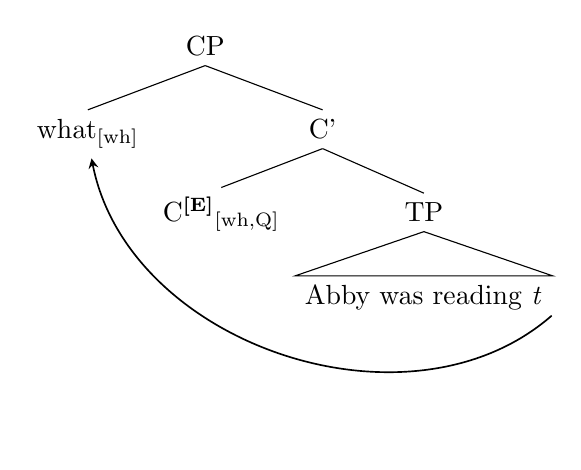
\begin{tikzpicture}[baseline]
   \tikzset{}
  \Tree[.CP \node(w){what\textsubscript{[wh]}}; [.C' C\textsuperscript{\textbf{[E]}}\textsubscript{[wh,Q]} [.TP \edge[roof]; {Abby was reading \textit{t}} ] ] ];
\draw[semithick, -stealth] (4.4,-3.3) to [bend left=60] (w);
\end{tikzpicture}

\caption{Derivation of the sluice in \ref{ex:merchant-sluicing} according to \citet[670]{merchant2004}.\label{fig:merchant-sluicing}}

\end{figure}
%
E\is{E feature} is always located on the head of a functional projection, like CP\is{Complementizer phrase} in Figure \ref{fig:merchant-sluicing}. The syntactic properties of E, which consist of a set of uninterpretable features, determine which head can host the feature. For instance, E\textsubscript{S}\is{E feature}, the E\is{E feature} feature found in sluicing, has the features [\textit{u}wh*, \textit{u}Q*] \citep[670]{merchant2004}. This ensures that it can be hosted only by heads that are [wh,Q] and that therefore can check these features, such as C in interrogatives. The variants of E\is{E feature} found in other types of ellipsis may have different feature specifications and are thereby restricted to other functional heads. \citet[671]{merchant2004} suggests that the varieties of E\is{E feature} are identical with respect to their phonology and semantics and differ only in these syntactic specifications. The phonological effect of the E feature\is{E feature} is that the complement of the head it is located on  remains unarticulated at PF. In \Last, this concerns the complete TP\is{Tense phrase} of the second conjunct in \Last. Both sentential accounts discussed so far, \citet{merchant2004} and \citet{reich2007}, agree that no syntactic structure is deleted during the derivation. Even though parts of it are unarticulated at PF, the unarticulated words are still present on LF. In \Last, this results in the wh-phrase being the only articulated word in the sluice, because it leaves the ellipsis site through \textit{wh}-movement to [Spec, CP\is{Complementizer phrase}].

According to \citet{merchant2004}, the licensing condition on omissions in fragments is \textit{e-givenness}\is{E-givenness}, which is included in the semantics of the E feature\is{E feature} \Next: E\is{E feature} requires the complement of the head hosting E\is{E feature} to be e-given\is{E-givenness}. E-givenness\is{E-givenness} is the identity condition licensing ellipsis in \citeauthor{merchant2001}'s theory and consists basically in a bidirectional givenness relation in the sense of \citet{schwarzschild1999}. An expression E counts as e-given\is{E-givenness} when it has a salient antecedent A which entails the existential closure of the focus value of A and vice versa. 

\ex. [[E]] = $\lambda$p: e-given (p) [p] \hfill \citep[672]{merchant2004}

The requirement for the complement of the head hosting E to be e-given\is{E-givenness} ensures that ellipsis is licensed only if there is a structural\is{Structural case}ly parallel antecedent available in context, and that it is blocked if there remains a constituent within the complement that is not e-given\is{E-givenness}. \Next exemplifies the mechanism for the sluicing\is{Sluicing} example in \LLast: The antecedent has the focus structure in \Next[a], whose existential closure \Next[b] is entailed by the sluice \Next[c]. As the existential closure of \Next[c] is identical to the one of the antecedent in \Next[b], the opposite relation also holds, so that the ellipsis in \LLast is licensed by e-given\is{E-givenness}ness.

\ex. \a. Abby was reading [something]\textsubscript{F}
     \b. $\exists$x. Abby was reading x
     \c. Abby was reading [what]\textsubscript{F}
     
\begin{figure}
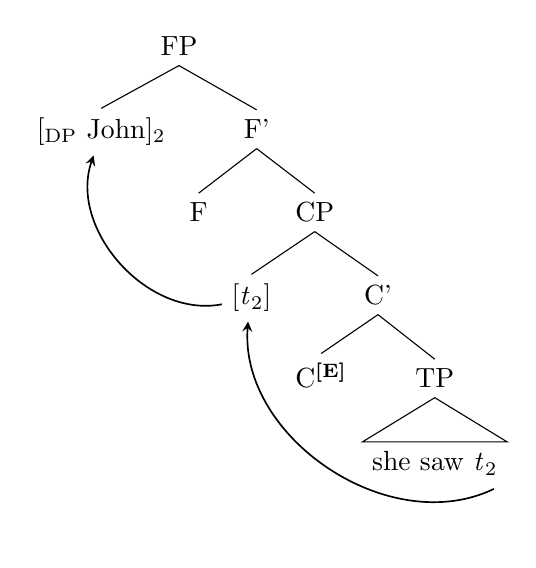
\begin{tikzpicture}[baseline]
   \tikzset{}
  \Tree[.FP \node(w){[\textsubscript{DP} John]\textsubscript{2}}; [.F' F [.CP \node(i){[\textit{t}\textsubscript{2}]}; [.C' C\textsuperscript{\textbf{[E]}} [.TP \edge[roof]; {she saw \textit{t}\textsubscript{2}} ] ] ] ] ];
\draw[semithick, -stealth] (i) to [bend left=60] (w);
 \draw[semithick, -stealth] (4,-5.5) to [bend left=60] (i);
\end{tikzpicture}

\caption{Derivation of the fragment answer in \ref{ex:merchant-shortanswer} according to \citet{merchant2004}.\label{ex:merchant.structure-full}}
\end{figure}
%
\citet{merchant2004} extends this analysis to fragments. His theory accounts for discourse-initial fragments\is{Fragment, discourse-initial} (see below for details), but he focuses mostly on short answer fragments\is{Fragment, short answer} like \Next, for which he assumes the structure in Figure \ref{ex:merchant.structure-full}. Again, the E feature\is{E feature} is hosted by C in the left periphery, while the fragment is moved to the specifier of a functional projection FP immediately above CP\is{Complementizer phrase}. This movement operation proceeds cyclically through [Spec, CP\is{Complementizer phrase}].

\ex. \a. Who did she see? \hfill \citep[673]{merchant2004}
\b. John.\label{ex:merchant-shortanswer}

The major difference between sluicing\is{Sluicing} and fragments is that E\textsubscript{F}, the variety of E\is{E feature} found in fragments, and E\textsubscript{S} have different syntactic features, which are [\textit{u}C*, \textit{u}F] for E\textsubscript{F} and [\textit{u}wh*, \textit{u}Q*] for E\textsubscript{S}. The strong \textit{u}C* feature ensures that E\is{E feature} is located on a C head, while the weak \textit{u}F feature can be checked under Agree \citep[707]{merchant2004}, because weak features don't need to be checked locally according to the theory. Otherwise, the derivation is identical to sluicing\is{Sluicing}: After the fragment has been moved, ellipsis applies to the TP\is{Tense phrase}.

With respect to the landing site of the fragment in [Spec, FP], \citeauthor{merchant2004} avoids committing himself to an analysis of what kind of projection FP is. However, \citet[675]{merchant2004} tentatively suggests that it is a focus projection in the sense of \citet{rizzi1997}.%
%
\footnote{Elsewhere \citep[703]{merchant2004} he relates the movement operation that results in fragments to Clitic Left Dislocation\is{Clitic left dislocation} (CLLD\is{Clitic left dislocation}, \citenob{cinque1990}) rather than to focus. See Section \ref{sec:theories-predictions-focus} for a discussion.}\afterfn%
%
%
\footnote{The idea that FP is a focus projection is further developed by \citet{gengel2007}, who argues explicitly that movement in fragments\is{Movement and deletion account} occurs to check a [$+$contrastive] feature in [Spec, FP]. This conclusion might be too strong, since in languages like German\is{German} or English\is{English} fronting foci is possible yet marked. Specifically, as \citet{weir2014} notes and I discuss in greater detail below, object DP\is{Determiner phrase} fragments are acceptable in situations where fronting objects is definitely not.}\afterfn
%
Whether or not FP is a focus projection is highly relevant to the theory, because this would provide an explanation for why movement in fragments\is{Movement and deletion account} would occur at all. Since \citeauthor{merchant2004}'s theory is embedded in a minimalist framework \citep{chomsky1995}, movement cannot be optional, but is a \textit{last resort} operation that is mostly driven by the need to check strong features in a local (specifier-head) configuration. In \citepos{merchant2001} account of sluicing\is{Sluicing}, the \textit{wh}-phrase reaches [Spec, CP\is{Complementizer phrase}] through \textit{wh}-movement, which is driven by uninterpretable features of the \textit{wh}-phrase. Similarly, movement in fragments\is{Movement and deletion account} requires a trigger which the E feature\is{E feature} cannot provide: Its syntax, as defined above, contains only uninterpretable features that determine on which head it can appear. If FP was related to an information-structural\is{Structural case}\is{Information structure} concept such as focus or topic, an uninterpretable feature related to this notion could trigger movement in fragments\is{Movement and deletion account} independently from E, just like \citet{merchant2001} argues for sluicing\is{Sluicing}.

From an empirical perspective, \citet{merchant2004} requires evidence that fragments have actually moved. Since he analyzes movement in fragments\is{Movement and deletion account} as regular A'-movement, his theory predicts that the derivation of fragments is subject to movement restrictions\is{Movement restriction} that are observed in full sentences: Only those constituents that can be moved to [Spec, FP] and appear in a left-peripheral position in full sentences are predicted to be possible fragments. \citet{merchant2004} presents introspective data from different phenomena and languages in support of this prediction, some of which will provide the testing ground for his theory in my experiments.%
%
\footnote{See Section \ref{sec:theories-predictions-movement} for details.}\afterfn%
%

However, \citet{weir2014} shows that the assumption that structures presumably underlying movement and deletion\is{Movement and deletion account} are acceptable across the board is falsified even by simple examples such as \Next. The short answer fragment\is{Fragment, short answer} in \Next[a] is fine despite the ungrammaticality of the presumably underlying fronting structure \Next[b]. The acceptability of left dislocation in a sentence seems not to be necessarily related to the acceptability of the corresponding fragment.
 
\ex. What did you eat?  \hfill \citep[168]{weir2014} \label{ex:weir-english-fronting}
\a. Chips.
\b. *Chips, I ate \textit{t}.

In order to account for such data while maintaining the idea of movement and deletion\is{Movement and deletion account}, \citet{weir2014} claims that movement in fragments\is{Movement and deletion account} is a special type of movement\is{Exceptional movement account} which is restricted to elliptical utterances and which differs from movement in narrow syntax, i.e. before spell out. According to \citeauthor{weir2014}, this \textit{exceptional} movement\is{Exceptional movement account} is triggered by a clash between the prosodic properties of focused expressions, which are marked with a pitch accent, and the ellipsis site, which the E feature\is{E feature} requires to be silent. As \citet{weir2014} assumes a similar underlying structure as \citet{merchant2004} does (see Figure \ref{ex:merchant.structure-full}), that is, a regular sentence whose C head hosts the E feature\is{E feature}, the TP\is{Tense phrase} is marked for PF-deletion, but still contains the focused DP\is{Determiner phrase} \textit{John}. This conflict is solved by moving the focused expression(s) out of the ellipsis site and adjoin\is{Adjunct}ing them to CP\is{Complementizer phrase}.

Exceptional movement\is{Exceptional movement account} differs from narrow syntactic movement. First, it is not driven by feature checking; in fact, \citet[195]{weir2014} denies that there is a focus feature in English\is{English}.%
%
\footnote{Focus fronting is still acceptable in English\is{English} if the focus is contrastive in the sense of \citet{krifka2007}, i.e., when alternatives to the focused expression are given in context \Next.

\ex. \textit{Him} I invited, not \textit{her}. \hfill

This could still be accounted for by a more specific feature that appears only in contrastive contexts. However, even in cases as \Last, focus fronting does not seem to be obligatory, therefore the English\is{English} data require closer investigation, specifically if movement is to be assumed as non-optional (provided the relevant features are present).}\afterfn%
%
According to \citeauthor{weir2014}, exceptional movement\is{Exceptional movement account} is nevertheless a last resort operation, because there is no other way of saving the derivation from crashing due to the clash between focus and ellipsis at PF. Second, exceptional movement\is{Exceptional movement account} has no effect on the semantics of the utterance. This is in line with the observation that, unlike \citet{gengel2007} suggests, fragments are not necessarily contrastive. \citet[183]{weir2014} attributes the absence of semantic effects of exceptional movement\is{Exceptional movement account} to its application after spell-out and at PF only. He argues that this also explains why it is restricted to elliptical utterances: The only purpose of exceptional movement\is{Exceptional movement account} is to evacuate focused constituents from the ellipsis site, and because focused constituents can remain in situ in full sentences, exceptional movement\is{Exceptional movement account} is ruled out by economy considerations.

As the discussion in Section \ref{sec:theories-predictions-movement} will show, the assumption of exceptional movement\is{Exceptional movement account} notably complicates the empirical evaluation of the movement and deletion\is{Movement and deletion account} account, because the strong correlation between the acceptability of fronting and fragments is no longer predicted. Therefore, the experiments presented below test \citepos{merchant2004} version of the theory\is{Movement and deletion account} in the first place, but I also discuss the relevance for the exceptional movement\is{Exceptional movement account} theory whenever its predictions differ from \citet{merchant2004}.
\is{Movement and deletion account|)}


\subsection{Discourse-initial fragments under sentential accounts} \label{sec:theories-initial}
\is{Fragment, discourse-initial|(}

Up to this point, the theoretical discussion has focused mostly on short answer fragments\is{Fragment, short answer}, although I argued in the introduction that the most uncontroversial instances of fragments are discourse-initial\is{Fragment, discourse-initial} ones. Discourse-initial fragments challenge any sentential account of fragments: Given the licensing conditions of ellipsis discussed so far, ellipsis requires an antecedent, and in examples such as \Next no such antecedent seems to be available. Nonsentential accounts\is{Nonsentential account} do not face this problem, as they derive the propositional meaning of fragments by pragmatic inference. Since some of the experiments presented in this work rely on discourse-initial\is{Fragment, discourse-initial} fragments, in what follows I discuss how sentential accounts can account for these utterances and some of their properties. In particular, I argue that in those situations where discourse-initial\is{Fragment, discourse-initial} fragments are used, an antecedent that licenses ellipsis can be retrieved from extralinguistic context\is{Context, extralinguistic}. This facilitates a unified sentential account of fragments with and without overt antecedents. 

\ex. \label{ex:fragments-dilang}
\a. [Passenger to taxi driver:] To the university, please! \label{ex:fragments-dilang-uni}
\b. [Customer to barista:] A coffee, please! \label{ex:fragments-dilang-coffee}
\c. [Taking a postcard out of the post box:] From John!\label{ex:fragments-dilang-letter}

Sentential accounts that assume a QuD-based\is{Question under Discussion} model of context \citep{reich2007, weir2014} can explain the utterances in \Last by assuming implicit QuDs\is{Question under Discussion}, which are evoked by the extralinguistic context\is{Context, extralinguistic} and which are appropriate antecedents \Next. For instance, a pedestrian approaching a taxi is likely to ask for a ride and a guest in the coffee shop is very likely to order a drink or some food. 

\ex.  
\a. $\langle$Where shall I take you?$\rangle$\label{ex:uni-taxi-qud}\\
	   \sout{Take me} to the university, please!
     \b. $\langle$What would you like to have?$\rangle$\\
	   \sout{I'd like to have} a coffee, please!
	   
\citet[1852]{reich2011} notes that such discourse-initial fragments\is{Fragment, discourse-initial} are \textit{indeterminate}, that is, there are several possible paraphrases of the missing material. For instance, the answer in \LLast[a] could be understood as \textit{Take me to the university!}, \textit{I'd like to go to the university.} or \textit{Drive to the university!}. \citeauthor{reich2011} takes this to be a defining feature of what he calls situation-based ellipsis (\textit{s-ellipsis})\is{Situation-based ellipsis}, for the resolution of which the hearer must resort to extralinguistic context\is{Context, extralinguistic}. In contrast, antecedent-based \textit{a-ellipses}\is{Antecedent-based ellipsis}, which have a linguistic antecedent\is{Context, linguistic} (e.g. gapping\is{Gapping}, right node raising\is{Right node raising} and VPE\is{Verb phrase ellipsis}), can be unambiguously resolved \Next.

\ex. John goes to the university and Mary \sout{goes} to the pub.

According to \citet[1852]{reich2011}, indeterminacy suggests that, unlike short answers\is{Fragment, short answer}, discourse-initial fragments\is{Fragment, discourse-initial} are syntactically genuine nonsententials. This implies a non-uniform analysis to fragments: If they have a linguistic antecedent\is{Context, linguistic}, like an explicit QuD\is{Question under Discussion} in the case of short answers\is{Fragment, short answer}, they are elliptical, and if they do not, they are nonsentential. However, in \citet{reich2007}, he notes that also in antecedent-based ellipsis\is{Antecedent-based ellipsis} like gapping\is{Gapping}, the focus structure of the second conjunct can vary. If there is wide focus on the first conjunct, different focus structures \Next and henceforth different omission patterns \NNext are possible in the second conjunct depending on which implicit QuD\is{Question under Discussion} is assumed.

\ex. \a. [John gave a book to \textit{Sue}]\textsubscript{F}, and John gave [a \textit{baseball}]\textsubscript{F} [to BILL]\textsubscript{F}. 
    \b. [John gave a book to \textit{Sue}]\textsubscript{F}, and [\textit{Peter}]\textsubscript{F} gave a book [to \textit{Ann}]\textsubscript{F}.\\ \mbox{}\hfill\hfill\citep[478]{reich2007}

\ex. \a. [John gave a book to \textit{Sue}]\textsubscript{F}, and [a \textit{baseball}]\textsubscript{F} [to \textit{Bill}]\textsubscript{F}. 
    \b. [John gave a book to \textit{Sue}]\textsubscript{F}, and [\textit{Peter}]\textsubscript{F} [to \textit{Ann}]\textsubscript{F}.\\ \mbox{}\hfill\hfill\citep[478]{reich2007}
    
\citet[477]{reich2007} argues that in such cases, ``a complete set of possible QuDs\is{Question under Discussion} [\dots] is reconstructed, from which the speaker chooses exactly one as the most salient.'' The hearer then has to figure out which QuD\is{Question under Discussion} out of this set is the one that the speaker had in mind. Besides extralinguistic context\is{Context, extralinguistic}, a strong cue toward the QuD\is{Question under Discussion} intended by the speaker is the form of the utterance: If only focused expressions survive gapping\is{Gapping}, \Last[a] will accommodate a QuD\is{Question under Discussion} as \textit{What did John give to whom?}  and \Last[b] \textit{Who gave a book to whom?}. This reasoning applies equally to fragments: If the hearer must infer which QuD\is{Question under Discussion} the speaker had in mind from context and the form of the elliptical utterance in gapping\is{Gapping}, there is no reason to assume that she is not able to infer the QuD\is{Question under Discussion} in case of fragments. The set of potential QuDs\is{Question under Discussion} might often be more restricted in case of gapping\is{Gapping} than in discourse-initial fragments\is{Fragment, discourse-initial} by the first conjunct, so that there might be a quantitative difference between the size of the set of possible QuDs\is{Question under Discussion} reconstructed in gapping\is{Gapping} and fragments. However, there is not necessarily a categorical difference between both constructions.

Furthermore, from a psycholinguistic perspective, the theories of fragments discussed so far are production accounts. What matters primarily to them is the speaker's perspective: Ellipsis is licensed if there is a QuD\is{Question under Discussion} in context which the speaker believes to be sufficiently salient. Since the hearer is aware of this, she knows that there must be such a contextually salient QuD\is{Question under Discussion} as soon as she realizes that the speaker's utterance is elliptical. If the speaker is cooperative or at least has the intention to get his message across \citep{grice1975, sperber.wilson1995}, he will only use a fragment when he believes that the QuD\is{Question under Discussion} is relatively easy to retrieve. For instance, if there is a high risk of being misunderstood due to several equally likely competing QuDs\is{Question under Discussion} that differ in meaning, the full sentence will be preferred. In fact, this is supported by the experiments on script knowledge\is{Script knowledge} in Chapter \ref{sec:chapter-infotheory-experiments} of this book. Consequently, indeterminacy of the meaning of a QuD\is{Question under Discussion} does not impede communication if fragments are used only when the QuD\is{Question under Discussion} is relatively predictable. Even if the meaning of the QuD\is{Question under Discussion} is retrievable, its lexicalization is not necessarily, as the set of semantically similar QuDs\is{Question under Discussion} listed above for the taxi example showed. However, communication can succeed even if the hearer fails to recover exactly the lexicalization of the QuD\is{Question under Discussion} that the speaker had in mind, as long as the recovered QuD\is{Question under Discussion} causes the hearer to perform the intended action. No matter which of the paraphrases the driver chooses in order to enrich the fragment in \ref{ex:uni-taxi-qud}, she will still carry the passenger to the university.

The difference between implicit and explicit QuDs\is{Question under Discussion} is furthermore specifically relevant to the hearer's perspective. If the speaker chooses to produce a fragment, he must have a particular QuD\is{Question under Discussion} in mind, be it implicit or explicit. Consequently, from his perspective there is no categorical difference between explicit QuDs\is{Question under Discussion} (in case of short answers\is{Fragment, short answer}) and implicit ones (in case of discourse-initial fragments\is{Fragment, discourse-initial}). Obviously, this changes from the perspective of the hearer, who has to reconstruct the missing material, because this task is  facilitated by a QuD\is{Question under Discussion}. Still though, as I noted above, a speaker who wants to get her message across will only choose to use the fragment if the effort\is{Processing effort} required for the hearer to infer the intended QuD\is{Question under Discussion} is reasonably small. This is confirmed by my experiments \ref{exp:scripts-rating} and \ref{exp:scripts-production}, which show that in particular predictable, that is, easily recoverable, words are omitted.

The assumption that the resolution of ellipsis might require some degree of inference is further supported by research on relatively uncontroversial instances of antecedent-based ellipsis\is{Antecedent-based ellipsis}. For instance, both gapping\is{Gapping} and VPE\is{Verb phrase ellipsis} allow for mismatches between the antecedent and target of ellipsis. The VPE\is{Verb phrase ellipsis} example in \Next[a] requires the hearer to reconstruct an active VP\is{Verb phrase} \textit{look into this problem} given a passive antecedent. Similarly, in gapping\is{Gapping}, hearers can reconstruct a plural verb given a singular antecedent \Next[b]. Therefore, rather than being a copy-and-paste process \citep{frazier.clifton2001}, the reconstruction of elided material seems to be a task that requires retrieving the omitted material from available contextual evidence and that becomes more effortful the more antecedent and target differ \citep{arregui.etal2006}.

\ex. \a. This problem was to have been looked into, but obviously nobody did $\langle$look into this problem$\rangle$.\hfill \citep[548]{kehler2002}
     \b. They are going to Chicago, and I $\langle$am going$\rangle$ to San Francisco.\\ \mbox{}\hfill \citep[755]{pullum.zwicky1986}

Taken together, a uniform analysis of discourse-initial\is{Fragment, discourse-initial} and short answer fragments\is{Fragment, short answer} as elliptical sentences is possible. Just like fragments, some antecedent-based ellipses\is{Antecedent-based ellipsis} require inferential reasoning about the omitted material, so that the difference between short answers and dis\-course-initial fragments is a gradual one: In the case of short answers, the missing material is explicitly given, so that its retrieval will be easier than in discourse-initial\is{Fragment, discourse-initial} fragments (on average). If such a uniform account explains the data equally well, it is simpler than a mixed account\is{Mixed account} that distinguishes between discourse-initial\is{Fragment, discourse-initial} fragments and short answers and consequently to be adopted unless there is evidence against it.

Unlike \citet{reich2007} and \citet{weir2014}, \citet{merchant2004} does not rely on the concept of QuD\is{Question under Discussion}, but his theory can also account for discourse-initial fragments\is{Fragment, discourse-initial}. Since e-givenness\is{E-givenness}, which licenses fragments in his theory, operates on semantic representations, fragments in principle require a salient linguistic antecedent. \citeauthor{merchant2004}'s account distinguishes between fragments that occur in highly conventionalized contexts like the taxi example \ref{ex:fragments-dilang-uni} and those which do not, like \Next[a]. In the case of highly predictive contexts, he notes that speakers have strong expectations about what is likely to happen and to be said in such contexts. \citet[730-731]{merchant2004} argues that this \textit{script knowledge}\is{Script knowledge} in the sense of \citet{schank.abelson1977}%
%
\footnote{See Section \ref{sec:infotheory-scripts} for details on the concept of script and a discussion of its psychological effects.}\afterfn%
% 
can make specific linguistic expressions manifest in the sense of relevance theory\is{Relevance theory}, that is, ``capable [\dots] of representing it mentally and accepting its representation as true or probably true'' \citep[39]{sperber.wilson1986}. Such manifest linguistic objects can then serve as antecedents and license omission if they result in parts of the utterance being e-given\is{E-givenness}\is{Context, extralinguistic}. For non-conventionalized cases, \citet[722-727]{merchant2004} argues that context can still make entities and concepts like the letter and its origin in \Next[a] manifest. This licenses the ellipsis of very basic deictic expressions, as the predicate \textit{do it} for actions and pronouns for entities in the structure in \Next[b] which he assumes for the fragment in \Last. 

\ex. \a. [Bill walks into the living room waving a postcard. He says:]
	   \sout{The postcard is} from John!
\b. From John \sout{it is}.

The deictic expressions are then resolved from context\is{Context, extralinguistic}, just like they are in regular sentences. \citet[722]{merchant2004} argues that the assumption that the unarticulated structure in such fragments consists in the minimally required and semantically less specified expressions also accounts for the indeterminacy of discourse-initial fragments\is{Fragment, discourse-initial}. Pronouns can be often paraphrased with various complex DPs\is{Determiner phrase}, so that this apparent property of fragments turns out to be just a more general property of deictic expressions. 

Taken together, the assumption that ellipsis can be licensed by extralinguistic context\is{Context, extralinguistic} provides an empirically necessary extension of the sentential account of fragments to (apparently) discourse-initial fragments\is{Fragment, discourse-initial}. Nonsentential accounts\is{Nonsentential account}, which rely on pragmatic inference in any case, do not face this problem, but might resort to the same mechanisms (e.g. script knowledge\is{Script knowledge} and implicit QuDs\is{Question under discussion}) in order to explain how fragments are interpreted.

\is{Fragment, discourse-initial|)}

\section{Fragments as ungrammatical utterances}  \label{sec:theories-ungrammatical}
\is{Ungrammaticality of fragments|(}

All of the theories discussed so far agree on the assumption that fragments are grammatical objects, be it by postulating mechanisms that license and trigger ellipsis or by modifying the theory in order to allow for nonsententials to be a well-formed output of syntax. This view is challenged by \citet{bergen.goodman2015}\is{Ungrammaticality of fragments}, who sketch a game-theoretic\is{Game theory} account of fragment usage and argue that fragments are actually ungrammatical, but that under some circumstances they might still be the preferred means of communicating a message. In simplified terms, \citeauthor{bergen.goodman2015} argue that hearers use a repair mechanism that helps to figure out the omitted parts of the utterance in order to infer the intended meaning from fragments. Such a mechanism is needed independently of fragments in order to deal with utterances that are corrupted by e.g. acoustic noise\is{Noisy channel}. Hearer and speaker are mutually aware of this possibility, so that the usage of a fragment and the subsequent inference about the intended meaning is more economic than that of a full sentence if the missing parts of the utterance are relatively easy to retrieve. Since this theory is highly usage-oriented and closely related to information theory\is{Information theory}, I discuss it in greater detail in Section \ref{sec:infotheory-uid}. For the time being, what matters is the presumed ungrammaticality of fragments.

Such an account predicts that there are no restrictions on the form of fragments, provided the chosen utterance is the most suitable for communicating a message in a specific context. In contrast, syntactic accounts categorically distinguish grammatical from ungrammatical fragments. Even though the acceptability of a grammatical fragment will also be determined to a large extent by context, there are grammatical principles that cannot be overridden. For instance, the movement restrictions\is{Movement restriction} that \citet{merchant2004} presents as evidence for his theory, or the requirement for fragments to be maximal XPs according to \citet{barton.progovac2005}, impose restrictions on the form of fragments that are context-independent.

It is hardly possible to empirically confirm the claim that fragments are ungrammatical objects, but it can be falsified by evidence for context-independent constraints on the form of fragments. The empirical picture is mixed: On the one hand, as my experiment \ref{exp:pstranding-defaultcase} will show, gradual differences in acceptability among ungrammatical fragments are in line with \citepos{bergen.goodman2015} account. On the other hand, there are grammatical constraints that override constraints that otherwise license omissions. For instance, \citet{lemke.etal2017} find that the omission of articles\is{Article omission} in German\is{German} newspaper headlines is subject to processing considerations that are related to those in \citet{bergen.goodman2015}\is{Game theory}. In standard German\is{German} however, including newspaper text, article omission\is{Article omission} is restricted only to very specific contexts (e.g. predicative and plural nouns). If grammaticality did not matter at all, the same amount of omissions would be expected in similar contexts across text types which are less constrained by normative pressures, like colloquial speech.

This objection concerns only the presumed ungrammaticality of fragments, but not the mechanism that \citet{bergen.goodman2015}\is{Ungrammaticality of fragments} propose in order to account for the speaker's choice between a fragment and a sentence. Such a mechanism is needed in any case,%
%
\footnote{See Section \ref{sec:fragments-game} for a more detailed sketch of such an account.}\afterfn%
%
because also when fragments are assumed to be grammatical the speaker must somehow decide on the form of the utterance. An account of this choice process is beyond the scope of generative\is{Generative grammar} syntactic theory, which does not attempt to model production preferences. Taken together, the main difference between the account in \citet{bergen.goodman2015}\is{Ungrammaticality of fragments} and syntactic theories of fragments concerns the question of whether the set of utterances that are possible in a situation is somehow constrained by syntax or derived by arbitrary omissions.%
%
\footnote{Note that \citet{bergen.goodman2015} do not discuss how this set of possible utterances is derived and present only a very simple example. Specifically, it is unclear whether they assume that fragments are genuine nonsententials or whether they take grammatical utterances as point of departure and generate the alternative by applying arbitrary ellipses to them.}\afterfn%
%
\is{Ungrammaticality of fragments|)}


\section{Testable predictions of theories of fragments}
\label{sec:theories-predictions}

The accounts discussed in the preceding section assume very different derivations of fragments and syntactic structures underlying them. However, all of them are designed to account in principle for the same acceptability data reported in the literature. Therefore, in order to evaluate their predictions empirically, it is necessary to isolate phenomena with respect to which these predictions differ. In this section, I present four such phenomena, which might provide a testing ground for the theories: case connectivity effects\is{Case connectivity}, discontinuous fragments, information-structural\is{Structural case}\is{Information structure} restrictions, and movement restrictions\is{Movement restriction}. As will turn out, only case connectivity and movement evidence will be useful to distinguish between the theories. With respect to constituency and focus marking, the theories either coincide for independent reasons or they do not make precise empirical predictions with respect to them at all.

\subsection{(Anti)connectivity effects: Case marking} \label{sec:theories-predictions-case}

\is{Case connectivity|(}
Both those authors who defend a sentential analysis of fragments and those supporting a nonsentential account\is{Nonsentential account} consider case connectivity effects\is{Case connectivity} to be an important diagnostic for the syntax of fragments. \citet[676--679]{merchant2004} presents evidence for connectivity effects\is{Case connectivity} from a diverse sample of languages. His general observation is that DP\is{Determiner phrase} short answers\is{Fragment, short answer} like the German\is{German} example \Next receive the same case morphology as their counterparts in complete sentences: Just like the \textit{wh}-phrase in the question, the DP\is{Determiner phrase} in the short answer has to receive accusative\is{Accusative case} case marking \Next[a], whereas the dative\is{Dative case} \Next[b] is ungrammatical. From the sententialist perspective, case connectivity provides indirect evidence for unarticulated structure: In minimalism\is{Minimalist program}, at least non-default case\is{Default case} must be checked in a local syntactic configuration between the DP\is{Determiner phrase} and another head, so the grammaticality of such a case marking indicates the presence of an unarticulated licensor. For instance, in \Next[a] accusative\is{Accusative case} must be checked by a verb, so that the acceptability of case marking in the absence of an overt verb suggests that the structure contains that verb, but that it has been PF-deleted in the course of the derivation. This pattern is reversed in \NNext, where the verb in the question requires dative\is{Dative case}. In this case, a dative\is{Dative case}, but not accusative\is{Accusative case}, DP\is{Determiner phrase} fragment is acceptable.

\exg. Wen sucht Hans?\label{ex:merchant.caseconn-acc}\\
who.\textsc{acc} seeks Hans\\
\trans{Who is Hans looking for?} \hfill \exsourceraised{\citep[677]{merchant2004}}
\ag. Den Lehrer.\label{ex:merchant.caseconn-acc-subex}\\ 
the.\textsc{acc} teacher \mbox{}\\
\bg. *Dem Lehrer.\\
the.\textsc{dat} teacher\\

\exg. Wem folgt Hans?\label{ex:merchant.caseconn-dat}\\
who.\textsc{dat} seeks Hans\\
\trans{Who does Hans follow?} \hfill \exsourceraised{\citep[677]{merchant2004}}
\ag. Dem Lehrer. \label{ex:merchant.caseconn-dat-subex}\\ 
the.\textsc{dat} teacher\\
\bg. *Den Lehrer.\\
the.\textsc{acc} teacher\\

Case connectivity effects\is{Case connectivity} thus support unarticulated structure in fragments. In contrast, as I already noted above, anticonnectivity effects\is{Case connectivity}, that is, mismatching case morphology between fragments and full sentences, support nonsentential accounts\is{Nonsentential account}. An example for anticonnectivity is the ungrammaticality of nominative\is{Nominative case} DP\is{Determiner phrase} fragments in the English\is{English} example \Next, although this case is required in the corresponding full sentence. Recall that \citet{barton.progovac2005} explained these data with the inability of fragments to exhibit structural case\is{Structural case} morphology under the assumption that nominative\is{Nominative case} is structural case\is{Structural case} in English\is{English}.

\ex. Who can eat another piece of cake? \hfill \citep[77]{barton.progovac2005} \label{ex:barton.case-rep}
\a. ?*I/?*We/?*He/?*She
\b. Me/Us/Him/Her

The introspective data reported in the literature is contradictory. \citeauthor{barton.progovac2005}'s example \Last exhibits anticonnectivity\is{Case connectivity}, but \citeauthor{merchant2004}'s German\is{German} examples in \ref{ex:merchant.caseconn-acc} and \ref{ex:merchant.caseconn-dat} seem to evidence case connectivity. Both sententialists and nonsententialists present explanations for at least part of the data that seems to contradict their respective theories. In what follows, I first review how the nonsentential account\is{Nonsentential account} could account for examples like \ref{ex:merchant.caseconn-acc-subex} and conclude that only the sentential account explains such connectivity effects. This rests on the assumption that accusative\is{Accusative case} is structural case\is{Structural case} in German\is{German}. This is supported by tests that \citet{progovac2006} use to show that Serbian\is{Bosnian/Croatian/Serbian} accusative\is{Accusative case} is inherent\is{Inherent case} case, but which yield the opposite result when they are applied to German. I then discuss how sentential accounts can deal with anticonnectivity\is{Case connectivity} effects as in \LLast. 

\subsubsection{Nonsentential accounts and connectivity}

As discussed above, \citet{progovac.etal2006} distinguish between default\is{Default case}, structural\is{Structural case} and inherent\is{Inherent case} case. In contrast to structural\is{Structural case} case feature\is{Case feature}s, which are uninterpretable, inherent\is{Inherent case} case feature\is{Case feature}s can and must be interpreted by semantics, because inherent\is{Inherent case} case is related to a specific \texttheta-role. The relatively uncontroversial claim that dative\is{Dative case} is inherent\is{Inherent case} case by \citet[339]{progovac.etal2006} explains the acceptability of dative\is{Dative case} DP\is{Determiner phrase} fragments as \ref{ex:merchant.caseconn-dat-subex}. In contrast, fragments that appear in structural\is{Structural case} case must be ungrammatical according to the nonsentential account\is{Nonsentential account}, because structural\is{Structural case} case feature\is{Case feature}s must be checked and structural\is{Structural case} case-marked DP\is{Determiner phrase} fragments lack an appropriate verbal head under a nonsentential analysis. This prediction is challenged by the acceptability of accusative\is{Accusative case} DP\is{Determiner phrase} fragments in German\is{German} \ref{ex:merchant.caseconn-acc-subex}, under the assumption that accusative\is{Accusative case} is structural\is{Structural case} case in German\is{German}.

\citet{progovac.etal2006} however argue that accusative\is{Accusative case} is not necessarily structural case\is{Structural case} in languages where nominative\is{Nominative case} is the default case\is{Default case}. They exemplify this idea for Serbian\is{Bosnian/Croatian/Serbian} and present three arguments that attempt to show that Serbian\is{Bosnian/Croatian/Serbian} accusative\is{Accusative case} is also inherent\is{Inherent case}, interpretable case. First, they note that an accusative\is{Accusative case} DP\is{Determiner phrase} ``is typically in fact a theme/patient'' \citep[339]{progovac.etal2006} and exclude a set of other \texttheta-roles for accusative\is{Accusative case}s (agent, goal/recipient, instrument, locative). As discussed above, the association with a specific \texttheta-role is the central criterion for categorizing a specific case as inherent\is{Inherent case} case. Second, they argue that in Serbian\is{Bosnian/Croatian/Serbian} accusative\is{Accusative case} contributes to semantics and present the contrast in \Next as evidence that accusative\is{Accusative case} has a universal quantificational meaning, while genitive\is{Genitive case} quantifies existentially. Finally, they state that, in contrast to English\is{English}, Serbian\is{Bosnian/Croatian/Serbian} accusative\is{Accusative case} objects do not always appear adjacent to the verb. This observation is not discussed in greater detail but is probably intended to suggest that no specific syntactic configuration is required for accusative\is{Accusative case} to be licensed.

\ex. \label{ex:serbian-case-quantification}
\ag. Dodaj vodu.\\
add water.\textsc{acc}\\
\trans{Add (all) the water.} \hfill \exsourceraised{\citep[340]{progovac.etal2006}}
\bg. Dodaj vode.\\
add water.\textsc{gen}\\
\trans{Add (some) water.}

Whether these arguments are empirically correct for Serbian\is{Bosnian/Croatian/Serbian} is beyond the scope of this book. However, if they applied to German\is{German} as well, this could derive grammatical accusative\is{Accusative case} DP\is{Determiner phrase} fragments like \ref{ex:merchant.caseconn-acc-subex} under a nonsentential account\is{Nonsentential account} and consequently undermine the status of case connectivity effects\is{Case connectivity} as evidence for unarticulated structure in fragments. 

Nevertheless, the diagnostics used by \citet{progovac.etal2006} to analyze the Serbian\is{Bosnian/Croatian/Serbian} accusative\is{Accusative case} as structural case\is{Structural case} do not yield the same result for the German\is{German} accusative\is{Accusative case}. The \texttheta-role argument that accusative\is{Accusative case} DP\is{Determiner phrase}s are typically themes or patients probably holds in German\is{German} too. For instance, it seems reasonable to assume that a random accusative\is{Accusative case} DP\is{Determiner phrase} drawn from a corpus\is{Corpus} is more likely to be a patient than a random nominative\is{Nominative case} DP\is{Determiner phrase} is. However, it is unclear how the gradual likelihood of being a patient can be aligned with the categorical distinction between structural\is{Structural case}, inherent\is{Inherent case} and default case\is{Default case} upon which \citepos{barton.progovac2005} theory relies. This probably concerns the Serbian data as well. The remaining two arguments for analyzing Serbian\is{Bosnian/Croatian/Serbian} accusative\is{Accusative case} as inherent\is{Inherent case} case do not hold in German\is{German}. Quantification relies on the presence of the definite article in German%
%
\footnote{This is evidenced by the German\is{German} counterparts of \ref{ex:serbian-case-quantification} in \Next. The adjective has accusative\is{Accusative case} case morphology in both examples but the meaning depends on the presence of the definite article.

\ex. \ag. Geben Sie den frischen Zitronensaft hinzu.\\
	  give.\textsc{imp} you the.\textsc{acc} fresh.\textsc{acc} lemon.juice to\\
	  \trans{Add (all of) the fresh lemon juice.}
    \bg. Geben Sie frischen Zitronensaft hinzu.\\
	  give.\textsc{imp} you fresh.\textsc{acc} lemon.juice to\\
	  \trans{Add (some of the) fresh lemon juice.}
	  
}\afterfn%
%
and accusative\is{Accusative case} DPs\is{Determiner phrase} still appear adjacent to the verb in the unmarked word order\is{Word order} in German\is{German}. This suggests that at least for German\is{German} the analysis of accusative\is{Accusative case} as structural case\is{Structural case} is correct. Consequently, if empirically confirmed, the acceptability of the accusative\is{Accusative case} DP fragments in German\is{German} challenges \citepos{barton.progovac2005} theory because it does indeed predict anticonnectivity effects\is{Case connectivity} in that case.%
%
\footnote{\label{fn:defaultcase-acc-pragmatics}Having defined Serbian\is{Bosnian/Croatian/Serbian} accusative\is{Accusative case} as inherent\is{Inherent case} case, \citet[340]{progovac.etal2006} argue that nominative\is{Nominative case} DP\is{Determiner phrase} fragments are degraded as answers to questions asking for an accusative\is{Accusative case} \Next for pragmatic reasons. They claim that the accusative\is{Accusative case} short answer\is{Fragment, short answer} is preferred over the nominative\is{Nominative case} one because it is more informative. This cannot explain the German\is{German} data: If accusative\is{Accusative case} is structural case\is{Structural case}, the only grammatical short answer\is{Fragment, short answer} is the nominative\is{Nominative case} one. The glosses and the grammaticality judgement in \Next[b] were added by  R.L. based on the text accompanying the example in \citet{progovac.etal2006}.

\ex. \label{ex:accusative-inherent-progovac} \ag. Koga je Ana posetila?\\
who.\textsc{acc} is Ana visited? \\
\trans{Who did Ana visit?}\hfill \exsourceraised{\citep[340]{progovac.etal2006}}
\bg. \#Vera!\\
Vera.\textsc{nom}\\

}\afterfn%
%
Experiment \ref{exp:case} disconfirms this prediction.

\subsubsection{Sentential accounts and anticonnectivity}
Anticonnectivity effects\is{Case connectivity} have been presented as evidence against sentential accounts, but at least some of the data can be explained by these theories. With respect to English\is{English} pronominal short answers\is{Fragment, short answer} discussed above, \citet[700--704]{merchant2004} reports similar data for Greek\is{Greek}, Dutch\is{Dutch}, German\is{German} and French\is{French}, which, aside from cross-linguistic differences, are characterized by formal differences between the pronouns found in fragments and those in full sentences. For instance, the French\is{French} data in \Next show that in fragments only the strong, tonic pronoun \textit{moi} is acceptable \Next[a], whereas the clitic \textit{me} must be used in regular sentences \Next[b].

However, \citeauthor{merchant2004} notes that in the left periphery only those pronouns that appear in fragments are acceptable. For instance, in Clitic Left Dislocation\is{Clitic left dislocation} (CLLD\is{Clitic left dislocation}) in French\is{French} \NNext[a] or hanging topic\is{Topic, hanging} left dislocation (HTLD)\is{Topic, hanging} in English\is{English} \NNext[b] the form of the pronoun matches the one found in short answers\is{Fragment, short answer}.

\exg. Il voulait qui?\\
he wanted who\\
\trans{Who did he want?}\hfill \exsourceraised{\citep[701]{merchant2004}}
\ag. Moi/*Me\\
me.strong/me.weak\\
\bg. Il me/*moi voulait.\\  
he me.weak/strong wanted\\
\trans{He wanted me}

\ex. \ag. Moi/*Me, il me voulait.\\
me.strong/weak he me wanted\\
\trans{Me, he wanted}\hfill \exsourceraised{\citep[702]{merchant2004}}
\b. Me/*I, I watered the plants. \hfill \citep[703]{merchant2004}

\citeauthor{merchant2004} argues that this is empirically in line with his theory, which assumes structures such as \Last to be the source of fragments. However, he is reluctant to assume HTLD\is{Topic, hanging} as the structure underlying fragments, because, unlike fragments, this construction is insensitive to island\is{Island}s. Instead, he suggests that the formal restrictions on pronominal fragments are due to the fact that weak pronouns cannot be focused. \citet{merchant2004} takes this as evidence for the movement component of his theory, but the observation that only pronouns which can be focused are possible fragments is perfectly in line with \citepos{reich2007} in situ ellipsis account\is{In situ deletion account}: \Next[a] shows that the English\is{English} pronoun \textit{me} can receive a pitch accent marking narrow or contrastive focus\is{Focus, contrastive}, whereas in French\is{French}, the tonic pronoun \Next[b] can but the clitic \Next[c] cannot. The deletion of all non-focused constituents under a semantic identity condition as proposed by \citet{reich2007} consequently yields the same pattern as movement and deletion\is{Movement and deletion account}.%
%
\footnote{Some authors account for mismatches between sentences and fragments with respect to preposition omission\is{Preposition omission} by deriving fragments from clefts\is{Cleft} (see e.g. \citet{rodrigues.etal2009} for Spanish\is{Spanish} and Brazilian Portuguese\is{Portuguese} and \citet{vancraenenbroeck2010} for English\is{English}). Under such an analysis, according to which accusative\is{Accusative case} in fragments evidences a connectivity effect\is{Case connectivity} than an anticonnectivity effect\is{Case connectivity}, \ref{ex:barton.cake} would be derived from a structure like \Next.

\ex. A: Who can eat another piece of cake?\\
     B: \sout{It's} me \sout{who can eat another piece of cake}

}\afterfn%
%
\footnote{The French data in \TextNext are also compatible with the nonsentential account\is{Nonsentential account}. Clitics like the French \textit{me} appear always adjacent to an inflected verb, which the nonsentential account argues to be absent in fragments. I thank Sebastian Nordhoff for pointing this out.}\afterfn%

\ex. A: Did they elect Ann?
\a. B: No, they elected \textit{me}.
\bg.  B: Non, ils ont élu \textit{moi}.\\
~~ no they have elected I.strong\\
\cg. B: *Non, ils \textit{me} ont élu.\\ 
~~ no they I.weak have elected\\

Taken together, the anticonnectivity effects\is{Case connectivity} observed by \citet{barton.progovac2005} for pronominal DP\is{Determiner phrase} short answers\is{Fragment, short answer} are explained not only by \citepos{barton.progovac2005} default case\is{Default case} hypothesis, but also by both types of sentential accounts. Case connectivity effects concerning inherent\is{Inherent case} case are also expected under both sentential and nonsentential accounts\is{Nonsentential account}.

What remains disputed is the possibility of case marking on full DP\is{Determiner phrase} fragments, which will serve as a diagnostic for unarticulated structure in my experiments. While sentential accounts predict case connectivity\is{Case connectivity} also for structural case\is{Structural case}, if the nonsentential account\is{Nonsentential account} is right, DP\is{Determiner phrase}s that receive structural case\is{Structural case} marking in full sentences appear in default case\is{Default case} in fragments. As noted by \citet{progovac.etal2006}, due to crosslinguistic variation, it is necessary to carefully determine whether a specific case is actually a structural case\is{Structural case} in a given language. Finally, if fragments are ungrammatical, as suggested by \citet{bergen.goodman2015}\is{Ungrammaticality of fragments}, no grammatical restrictions on case marking in fragments are expected. Still though, case in fragments should tend toward matching that in the corresponding sentence, because it is a strong cue toward the meaning intended by the speaker.
\is{Case connectivity|)}

\subsection{Constituency}\label{sec:theories-predictions-constituents}
The theories presented in the previous section disagree on whether fragments must be a single constituent: The nonsentential account\is{Nonsentential account} by \citet{barton.progovac2005} as well as movement and deletion\is{Movement and deletion account} predict this, but in situ deletion\is{In situ deletion account} and \citepos{bergen.goodman2015} approach allow for non-constituent fragments. 

\subsubsection{Constituency under the nonsentential account}
\citet{barton.progovac2005} argue that any maximal projection XP can be a well-formed output of syntax, therefore a fragment must always consist of a single constituent of arbitrary size and internal complexity. Sequences of constituents that do not have a unifying node cannot be derived. The examples discussed in \citet{barton.progovac2005} clearly conform to this restriction. \citet{progovac2006} discusses more controversial examples like \Next, which are harder to analyze as a single constituent, because the predicate \textit{a bargain} does not have a verbal projection, whose specifier could host the subject.

\ex. This a bargain!? \hfill \citep[28]{progovac2006} \label{ex:progovac.sc-bargain-root}

In order to account for such apparent DP\is{Determiner phrase}-DP\is{Determiner phrase} sequences too, which in fact are relatively frequent \citep{reich2017}, \citet{progovac2006} resorts to a small clause\is{Small clause} analysis. Small clauses\is{Small clause} \citep{williams1975, stowell1981} are expressions that contain a subject and a predicate, but no verbal material. They can appear as root small clauses \Last or be embedded as verbal complement inside a matrix clause \Next.

\ex. I consider this a bargain. \hfill \citep[41]{progovac2006} \label{ex:progovac.sc-bargain-embedded}

\begin{figure}
\begin{minipage}{.3\textwidth}
\begin{center}
   \Tree [.DP This [.D' [.D a ] [.N bargain ] ] ]
   
\end{center}
\end{minipage}
\begin{minipage}{.02\textwidth}
~~
\end{minipage}
\begin{minipage}{.3\textwidth}
\begin{center}
  \Tree [.PP Class [.P' [.P in ] [.N session ] ] ]
  
\end{center} 
\end{minipage}
\caption{DP and PP small clauses according to \citet[39]{progovac2006}.\label{p06-smallclause}}
\end{figure}
%
\citet[61]{progovac2006} claims that ``every sentence/clause is underlyingly a small clause.'' The subject is merged into the specifier of a projection whose category is determined by the predicate, as the examples in Figure \ref{p06-smallclause} illustrate.%
%
\footnote{This analysis can be traced back to \citet{stowell1981}, see \citet{citko2011} for an overview of alternative structural\is{Structural case} analyses of small clauses.}\afterfn%
%
If the small clause\is{Small clause} analysis is correct, it enables the nonsentential account\is{Nonsentential account} to derive XP-YP sequences as small clauses\is{Small clause}, as long as they do not contain uninterpretable features. \citet[51]{progovac2006} argues that the latter condition is met, because the subjects of root and embedded small clauses in English\is{English} appear in accusative\is{Accusative case} default case\is{Default case} \Next[a], which does not need to be checked according to the nonsentential account\is{Nonsentential account}. If the small clause\is{Small clause} serves as input to a regular inflected clause \Next[b] instead, the subject is selected from the lexicon with nominative\is{Nominative case} case features\is{Case feature} that are checked as usual in course of the derivation by T. In the embedded \Next[c], case is checked through ECM by the verb \citep[46]{progovac2006}. 

\ex. \a. Her give up?! (Never!) \hfill \citep[41]{progovac2006} \label{ex:progovac.sc-give-up-root}
     \b. She gives up?!
     \c. I never saw her give up.

This analysis works for the (mostly) English\is{English} examples discussed by \citet{progovac2006}, but there are instances of fragments for which the small clause\is{Small clause} analysis fails. For instance, the German\is{German} fragment in \Next[a] seems to be acceptable just like its English\is{English} counterpart \ref{ex:progovac.sc-bargain-root} is, but, unlike in English\is{English} \ref{ex:progovac.sc-bargain-embedded}, it cannot be embedded under a verb in a matrix clause \Next[b]. Instead, the complement must be a clause headed by a copula \Next[c]. \citet{reich2017} presents further arguments against a small clause\is{Small clause} analysis of German\is{German} XP-YP fragments, which are based on corpus\is{Corpus} data from newspaper headlines. He concludes that such cases involve a null copula and consequently analyzes \Next[a] as underlyingly sentential.

\ex. \ag. Das ein Angebot?!\\ 
	  this a bargain\\
     \bg. *Ich finde das ein Angebot.\\
	 I find this a bargain\\
	 \trans{I consider this a bargain.}
    \cg. Ich finde, das ist ein Angebot.\\
	I find this is a bargain\\

Furthermore, in question-answer pairs like \ref{ex:theories-discontinuous-en-pizza}, repeated here as \Next, fragments can consist of two non-predicative DPs\is{Determiner phrase} with an omitted main verb. A small clause\is{Small clause} analysis is ruled out in this case, because the missing verbal element is not the copula. It is unclear how \citet{barton.progovac2005} would account for such fragments without assuming an unarticulated verbal node, ellipsis, or a discontinuous fragment, which their account cannot derive.
 
\ex. [Waiter to customers in the restaurant:] Who ordered what?\\
Customer: She \sout{ordered} the deep dish pizza. 

The nonsentential account\is{Nonsentential account} hence predicts that only expressions consisting of a single constituent are possible fragments. Otherwise, the grammar assumed by \citet{barton.progovac2005} would not be able to generate them. \citepos{progovac2006} small clause\is{Small clause} analysis accounts for some apparent non-constituent fragments, but presupposes that small clauses\is{Small clause} are grammatical in the a language. The comparison between German\is{German} and English\is{English} suggests that similar fragments are acceptable in both languages even though the small clause\is{Small clause} analysis does not account for the relevant data in German\is{German} \citep{reich2017}. Furthermore, \Last suggests that even in English\is{English} not all fragments can be traced back to a small clause\is{Small clause}.

\subsubsection{Constituency under sentential accounts}
\citepos{merchant2004} movement and deletion\is{Movement and deletion account} account also predicts that fragments are always single constituents. As their derivation involves movement to [Spec, FP] for feature checking purposes, only one constituent can be moved at a time. The reason for this is that there is only one landing site for the fragment: the specifier of a head carrying the E feature\is{E feature}.%
%
\footnote{If multiple specifiers are assumed, as the minimalist program permits \citep[285]{chomsky1995} this restriction obviously does not hold anymore. However, \citet{merchant2004} does not seem to resort to multiple specifiers in order to explain apparent non-constituent fragments.}\afterfn
%
Of course, there are no restrictions on the internal complexity of this constituent, so that \citet{merchant2004} can account for small clause\is{Small clause} \ref{ex:progovac.sc-give-up-root} or VP\is{Verb phrase} fragments \Next:

\ex. What would you like to do tonight?\\ \label{ex:vp-fronting}
Go to the cinema\sout{, I'd like to}.

As \citet{merchant2004} allows for unarticulated structure in his elliptical sentences, the set of apparent non-constituent fragments that his account can explain is larger than that covered by the nonsentential account\is{Nonsentential account}. For instance, a sequence of a temporal and a locative adverbial\is{Adverbial} does not form a small clause\is{Small clause} but seems to be felicitous as a fragment \Next. For the movement and deletion\is{Movement and deletion account} account to derive such fragments, they need to form a single constituent at some point of the derivation. The assumption that this is possible in case of such adverbial\is{Adverbial}s is supported by German\is{German} data from \citet{haider2000}. \citeauthor{haider2000} observes that such \textit{clusters} consisting of event-related adverbial\is{Adverbial}s, may appear together in the German\is{German} sentence-initial prefield\is{Prefield} \NNext, which is generally considered to host only one constituent (see also the discussion of experiment \ref{exp:mvb} in Section \ref{sec:mvb-background}).%
% 
\footnote{\citet[104-105]{haider2000} also rules out an alternative derivation that fronts the complete VP\is{Verb phrase} after extracting the verb for independent reasons, but cf. \citet{muller2004} for such a proposal.}\afterfn%
%

\ex. Q: When did you last meet him?\\
    A: Last night in the pub.

\exg. Gestern im Hörsaal als der Vortrag begann hustete er wie verrückt.\\
yesterday in.the lecture.room when the lecture started coughed he like mad\\
\trans{Yesterday in the lecture room as the lecture started he coughed like mad.}\\\mbox{}\hfill\raisebox{3\baselineskip}[0pt][0pt]{\citep[104]{haider2000}}

\vspace{-11pt}
A similar point is made by \citet{muller2002} in his analysis of (apparent) multiple prefield\is{Prefield} constituents in German\is{German}. As pointed out above, German\is{German} declarative matrix clauses are verb-second (in what follows, V2), so that only one constituent may precede the inflected verb. In spite of this, \citet{muller2002, muller2003, muller2005} reports a diverse sample of corpus\is{Corpus} data which seem to violate this constraint. For instance, in \Next, taken from \citet[38]{muller2005}, a locative and a temporal PP\is{Preposition phrase}, which do not straightforwardly form a single constituent, can appear together in the prefield\is{Prefield}.%
%
\footnote{Note that, unlike \ref{ex:vp-fronting}, this example does not involve fronting of the complete VP\is{Verb phrase}.}\afterfn%
%
\citet{muller2002} develops a HPSG\is{HPSG} account of such data, whose central assumption is that the prefield\is{Prefield} consists of a single constituent which is headed by an unarticulated verb.

\exg. [Vor drei  Wochen] [in Memphis] hatte Stich noch in drei Sätzen gegen Connors verloren.\\ 
ago three weeks    in Memphis  had   Stich  still   in three sets   against Connors lost\\
\trans{Three weeks ago in Memphis Stich had still lost in three sets against Connors.}

The exact predictions of the movement and deletion\is{Movement and deletion account} account thus depend to a large extent on how many and which movement operations and covert elements are assumed in general, therefore it is difficult to derive testable predictions unless there is consensus on these preliminary assumptions. The picture becomes even more complicated if a fine-grained left periphery is assumed. Even in the original sketch of the CP\is{Complementizer phrase} layer in \citet{rizzi1997} there is a further topic projection above FocP, and \citet{beninca.poletto2004} distinguish about half a dozen highly specified functional projections, most of which are located above those related to focus. Depending on where \citet{merchant2004} would locate the E feature\is{E feature} in a language, the material in these projections could survive ellipsis, so that (if these projections exist in a language) the movement and deletion\is{Movement and deletion account} account predicts the possibility of genuine non-constituent fragments in highly specific information-structural\is{Structural case}\is{Information structure} configurations. Finally, the version of movement and deletion\is{Movement and deletion account} by \citet{weir2014} also accounts for non-constituent fragments. \citeauthor{weir2014} simply adjoins\is{Adjunct} the moved constituents to CP\is{Complementizer phrase} and, since adjunction is recursive, there is no upper bound limit on the number of constituents extracted with this mechanism.

Taken together, the existence of (apparently) discontinuous fragments as evidence for or against specific accounts of fragments does not seem promising, because theories that in principle predict constituency to be a determining property of fragments can account for some instances of what superficially must be classified as non-constituents. Specifically, movement and deletion\is{Movement and deletion account} requires an extensive set of preliminary assumptions about which syntactic operations and functional projections are available in a given language in order to make clear predictions on non-constituent fragments. Therefore, I do not use constituency directly as a diagnostic for particular theories.%
%
\footnote{An exception is experiment \ref{exp:mvb}, which compares the acceptability of apparent multiple prefield\is{Prefield} configurations as fragments and full sentences. However, the experiment does not depend on a specific syntactic analysis of the constructions tested, but on the parallelism between fragments and left dislocations predicted by the movement and deletion\is{Movement and deletion account} account.}\afterfn%
%

\subsection{Information structure and focus}
\is{Information structure|(}
\label{sec:theories-predictions-focus}
All sentential accounts of fragments discussed so far \citep{merchant2004, reich2007, weir2014} assume that information structure\is{Information structure}, in particular the focus-background structure of an utterance, determines which words can be omitted in fragments. Since the nonsentential account of fragments does not impose information-structural licensing conditions on fragments, focus-sensitivity could appear to be a promising testing ground to differentiate between sentential and nonsentential accounts\is{Nonsentential account}. \citet{reich2007} and \citet{weir2014} make the strongest claim on the issue by assuming that fragments are necessarily focused. \citeauthor{reich2007} argues that only F-marked\is{F-marking} expressions survive ellipsis, whereas \citeauthor{weir2014} considers focus to trigger exceptional movement\is{Exceptional movement account}.%
%
\footnote{If there is more than one focus, their predictions might differ with respect to ordering. \citet{reich2007} predicts the same ordering as in regular sentences, but for \citeauthor{weir2014}'s theory it matters whether several exceptional movement\is{Exceptional movement account} operations proceed from the top of the syntax tree to its bottom or vice-versa. E\is{E feature} is located on the C head dominating the whole TP\is{Tense phrase}, so that if the constituents closest to E\is{E feature} were evacuated first, both accounts would predict differing orderings.}\afterfn%
%

As for \citet{merchant2004}, this is less clear: On the one hand, he tentatively suggests identifying the landing site for fragments as a FocP \citep[675]{merchant2004}, on the other hand he emphasizes similarities between fragments and CLLD\is{Clitic left dislocation} \citep[703]{merchant2004}. However, according to the literature on CLLD\is{Clitic left dislocation}, this construction does not involve focus movement but targets a topic position.%
%
\footnote{\citet[53]{beninca.poletto2004} distinguish between topic and focus positions in the left periphery by noting that the former ``are connected with a clitic or a \textit{pro} in the sentence'', while the latter leave a variable which is bound by the moved phrase. Based on mostly Spanish\is{Spanish} data, \citet{arregi2003} argues that CLLD\is{Clitic left dislocation}ed constituents are contrastive topics\is{Topic, contrastive}. Contrastive topics differ from foci both in their syntactic properties and in their prosody \citep[see e.g.][]{buring1997, krifka2007}.}\afterfn%
%
Further confusion on the status of the presumed left dislocation of fragments comes from the German\is{German} data in \Next. \citet[702]{merchant2004} argues that the form of pronouns in the preverbal position (the \textit{prefield}\is{Prefield}) equals that in the fragments in \NNext (judgments are \citeauthor{merchant2004}'s). 

\exg. Was wolltest du?\\
     what wanted you\\
     \trans{What did you want?} \hfill \exsourceraised{\citep[701]{merchant2004}}
\ag. {Das/*Es} wollte ich.\\
    this/it wanted I\\
    \trans{This/It I wanted.} \hfill \exsourceraised{\citep[702]{merchant2004}}
\b.  Das/*Es.

\ex. *Das\textsubscript{i}/*Es\textsubscript{i} wollte \sout{ich \textit{t}\textsubscript{i}}.

The structure in \LLast[a] is derived neither by CLLD\is{Clitic left dislocation} nor by focus movement, because it is a garden-variety verb-second declarative matrix clause. As I discuss in greater detail in Section \ref{sec:mvb-background}, the mainstream analysis of German\is{German} V2 consists in moving the inflected verb to C, whose specifier must be filled by any other constituent \citep{denbesten1989}. Crucially, there are almost no restrictions on the category or information-structural\is{Information structure} status of the constituent in [Spec, CP]\is{Complementizer phrase}, which can be an aboutness or contrastive topic\is{Topic, contrastive} as well as a focus \citep{frey2005}. If \LLast[a] is a standard verb-second clause and the mainstream analysis of V2 is correct,%
%
\footnote{\citet{muller2004} proposes an analysis of V2 that consists in VP\is{Verb phrase} fronting after those constituents that appear in post-verbal positions have been extracted. As he assumes that the VP\is{Verb phrase} contains only the finite verb and the prefield\is{Prefield} when it is fronted, it makes the same predictions as the mainstream account of V2, that is, the verb must survive ellipsis in fragments.}\afterfn%
%
the fragment in \Last[b] cannot be derived from \Last[a] by assuming an E feature\is{E feature} on C: E\is{E feature} triggers only PF-deletion of the complement of C, hence the account incorrectly predicts the verb to survive ellipsis:%
%
\footnote{A possible explanation would be that T-to-C movement of the verb occurs only in order to satisfy some PF constraint and is therefore not required (which is equivalent to not being allowed in minimalism\is{Minimalist program}) in elliptical sentences. I am not aware of any proposal in this direction.}\afterfn%
%
Furthermore, the structure in \LLast[a] is not an instance of CLLD\is{Clitic left dislocation}. Even though German\is{German} declarative matrix clauses are verb-second, a further constituent can be placed left of the prefield\is{Prefield} \Next. DPs\is{Determiner phrase} appearing there sometimes exhibit no case connectivity\is{Case connectivity} at all \Next[a] and must therefore be analyzed as a hanging topic\is{Topic, hanging} \citep{rodman1974, vat1981}, but in \Next[b] the DP \textit{den Peter} resembles CLLD\is{Clitic left dislocation} in being case-marked. Unlike \LLast[a], both of these structures require doubling of the left-peripheral constituent by a pronoun.

\ex. \ag. Der Peter, den habe ich gestern erst getroffen.\\
	  the.\textsc{nom} Peter, him have I yesterday just met.\\
	  \trans{(As for) Peter, I just met him yesterday.}
     \bg. Den Peter, den habe ich gestern erst getroffen.\\
     	  the.\textsc{acc} Peter, him have I yesterday just met.\\
	  \trans{Peter, I just met him yesterday.}

However, the structure in \Last[b] cannot be the source of fragments. If E\is{E feature} is located on C, again, both the verb and the pronoun would survive ellipsis. The derivation in Figure \ref{fig:merchant-spec-cp} shows that this would yield the ungrammatical \textit{*Den Peter, den habe}. Taken together, E\is{E feature} cannot be located on C in German\is{German}.
%
\begin{figure}[t]
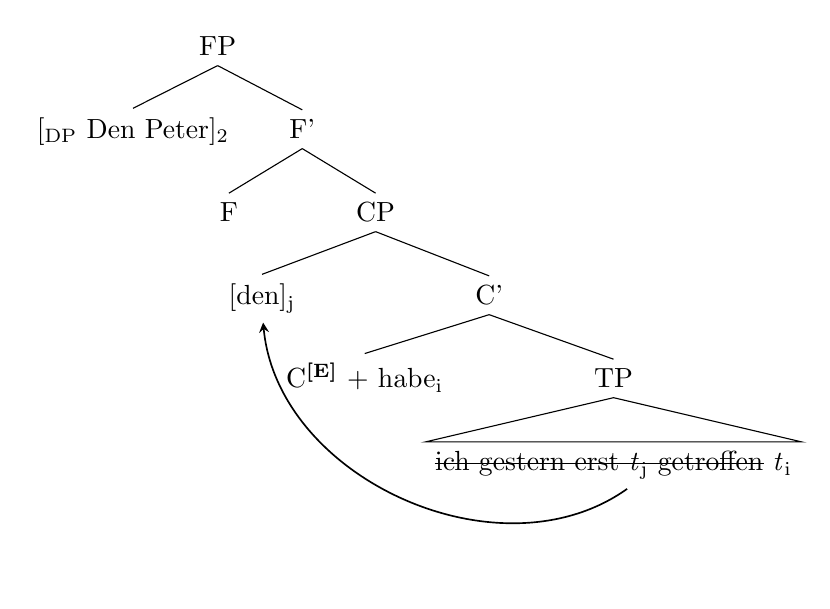
\begin{tikzpicture}[baseline,sibling distance=-10pt]
   \tikzset{}
  \Tree[.FP \node(w){[\textsubscript{DP} {Den Peter}]\textsubscript{2}}; [.F' F [.CP \node(i){[den]\textsubscript{j}}; [.C' {C\textsuperscript{\textbf{[E]}} + habe\textsubscript{i}} [.TP \edge[roof]; {\sout{ich gestern erst \textit{t}\textsubscript{j} getroffen} \textit{t}\textsubscript{i}} ] ] ] ] ];
 \draw[semithick, -stealth] (5.2,-5.5) to [bend left=60] (i);
\end{tikzpicture}

\caption{The derivation shows that if the E feature was located on [Spec, CP], German finite words are incorrectly predicted to survive ellipsis in fragments.\label{fig:merchant-spec-cp}}
\end{figure}
%
\citet{merchant2004} specifies the syntactic properties of different varieties of E\is{E feature} in their lexical entries, so there is no principled reason to assume that the German\is{German} E\textsubscript{F}\is{E feature} must also be [\textit{u}C*]. If it had an [\textit{u}F*] feature and were thus located on F, as \citet{merchant2004} initially suggested for English\is{English}, the verb would always be PF-deleted and the existence of DP\is{Determiner phrase} fragments straightforwardly explained. The problem with this assumption is that \citet{merchant2004} rejected it in order to account for the island\is{Island} sensitivity of fragments based on the PF-deletion of illegal traces\is{Trace (movement)} (see Section \ref{sec:theories-predictions-movement} for discussion). Therefore, if the E feature\is{E feature} was located on a F head above CP\is{Complementizer phrase} in German\is{German}, German\is{German} fragments should not be island-sensitive\is{Island}, but \Next shows that they are.%
%
\footnote{\citet{merchant2004} judges the English counterpart of \ref{ex:merchant-island-ger-shortanswer} as ungrammatical when it is interpreted as \Next[a]. If \ref{ex:merchant-island-ger-shortanswer} was interpreted as \Next[b], he predicts the fragment to be grammatical, because fronting \textit{Charlie} in the matrix clause does not require the extraction out of an island.

\ex. \ag. Nein, Abby spricht die gleiche Balkansprache, die Charlie spricht.\\
	 no Abby speaks the same balkan.language that Charlie speaks\\
	 \trans{No, Abby speaks the same Balkan language that Charlie speaks.}
     \bg. Nein, Charlie spricht die gleiche Balkansprache, die Ben spricht.\\
     	 no Charlie speaks the same balkan.language that Ben speaks\\
       \trans{No, Charlie speaks the same Balkan language that Ben speaks.}
       
}
\afterfn%
%

\ex. \ag. Spricht Abby die gleiche Balkansprache, die \textit{Ben} spricht?\\
	  speaks Abby the same balkan.language that Ben speaks\\
	  \trans{Does Abby speak the same Balkan language that \textit{Ben} speaks?}
\bg. *Nein, \textit{Charlie}.\label{ex:merchant-island-ger-shortanswer}\\
      no Charlie\\
      \trans{No, Charlie}\exsourceraised{\citep[translated from][708]{merchant2004}}

Taken together, the predictions of \citet{merchant2004} with respect to focus marking\is{F-marking} are vague, because it is not totally clear whether he assumes fragments to target the focus position [Spec, FP] or whether their landing site is [Spec, CP]\is{Complementizer phrase}. Neither of these versions can account for the full range of the data discussed in this section. The exceptional movement\is{Exceptional movement account} version of the theory \citep{weir2014} does not require information structure\is{Information structure}-related projections as FocP but simply adjoins\is{Adjunct} fragments to CP\is{Complementizer phrase}, so that it is not affected by these issues.

Nonsentential accounts\is{Nonsentential account} do not make reference to focus, but the conditions on fragment use that they require are related to information-structural\is{Information structure} notions. \citet{barton1990} proposes to ``delete up to recoverability'' and \citet{stainton2006} requires that a salient nonlinguistic LF which allows to enrich the fragment to a proposition must be present in context. As foci tend toward being new and consequently not recoverable, both of these ideas make similar predictions with respect to the acceptability of fragments as a focus-based account.

Focus sensitivity therefore does not offer a promising testing ground to distinguish the predictions of the theories of fragments that I investigate. Besides that, the effect of focus is relatively difficult to investigate experimentally. In German\is{German} and English\is{English}, focus is often marked prosodically with a H* pitch accent \citep{gussenhoven1983, pierrehumbert.hirschberg1990} and the prominence of prosodic focus marking varies gradually as a function of the size of the focus domain \citet{baumann.etal2006, baumann.etal2007}. This is hard to manipulate experimentally: As \citet{baumann.etal2007} report, speakers make use of different strategies to modulate the prosodic prominence of foci, so that items might not be understood as intended. Furthermore, while work in experimental pragmatics has provided evidence for an effect of pitch accents on interpretation of complete sentences \citep[see e.g.][]{chevallier.etal2008, zondervan2010}, it is difficult to apply this to fragments. For instance, in DP\is{Determiner phrase} fragments consisting only of a noun and an article, the most prominent accent always falls on the noun, hence it is not possible to vary the pitch accents on fragments in order to elicit different focus structures.
\is{Information structure|)}


\subsection{Evidence for movement}
\label{sec:theories-predictions-movement}
\is{Movement restriction|(}

In contrast to any of the other accounts, \citepos{merchant2004} theory requires fragments to undergo obligatory movement to a left-peripheral position. From a na\"{i}ve perspective, this predicts that only expressions that can occur in a left-peripheral position, more specifically, to the left of the head hosting the E feature\is{E feature}, are possible fragments. Consequently, whatever might restrict movement to the left periphery in full sentences will also constrain the form of fragments. In the next chapter, I empirically investigate two of the movement restrictions\is{Movement restriction} discussed by \citet{merchant2004}. These restrictions, whose effects on the form of fragments have been first tested in \citet{merchant.etal2013}, concern complement clause\is{Complement clause} topicalization and preposition stranding\is{Preposition stranding}. The reason for choosing these phenomena is that \citet{merchant.etal2013} present the first experimental evidence on them, what suggests that they consider them a valid testing ground for the movement and deletion account\is{Movement and deletion account}. Preposition stranding restrictions have the additional advantage that they cannot be overridden by exceptional movement\is{Exceptional movement account} according to \citet{weir2015} and hence also allow us to test \citepos{weir2014} version of the theory.

The idea that movement restrictions\is{Movement restriction} constrain the form of fragments is exemplified for complement clause\is{Complement clause} topicalization in \Next and \NNext, from \citet[690]{merchant2004}: As has been repeatedly claimed in the theoretical literature \citep[see e.g.][]{morgan1973, chomsky1981, stowell1981, webelhuth1992}, the complementizer in English\is{English} non-factive\is{Factivity} complement clause\is{Complement clause}s is optional when the complement clause\is{Complement clause} appears in its base position \Next[a], but becomes obligatory when the complement clause\is{Complement clause} appears in the left-periphery \Next[b]. \citet{merchant2004} observes that the same holds for fragments \NNext. He concludes that this is unexpected under the in situ deletion\is{In situ deletion account} account, because the complementizer would be optional in fragments too if their underlying structure was \Next[a] instead of \Next[b]. The other movement restrictions\is{Movement restriction} discussed by \citet{merchant2004} behave similarly, that is, expressions which cannot appear in the left periphery seem to be unacceptable as fragments. 

\ex. \label{ex:merchant.teacher-sent}
\a. No one believes (that) I’m taller than I really am. 
\b. *(That) I’m taller than I really am, no one believes.

\ex. \label{ex:merchant.teacher-frag}
What does no one believe? \hfill \citep[690]{merchant2004}\\
\mbox{}\hspace{-.45em}\#(That) I’m taller than I really am.

\citet{merchant2004}\is{Movement and deletion account} interprets such data as evidence in favor of his account, but in order for this to constitute valid evidence for movement in fragments\is{Movement and deletion account}, it is necessary to rule out alternative explanations for the observed pattern, which do not require movement. Throughout this book, some of these data will turn out to be relatively straightforwardly captured by the nonsentential or the in situ deletion\is{In situ deletion account} accounts. For instance, a construction might have properties that block both movement in full sentences and ellipsis in fragments without having to assume that the latter necessarily undergo movement.

Besides this need for caution when interpreting coincidences between fragments and left dislocation as evidence for movement, acceptable fragments that cannot be left-dislocated potentially constitute counterevidence to \citepos{merchant2004} theory. If ungrammatical left dislocations in full sentences always yielded unacceptable fragments, movement and deletion\is{Movement and deletion account} would be falsified even by the most basic examples, such as the unavailability of fronting of a DP\is{Determiner phrase} which is not contrastive in English\is{English} \citep{weir2014}, or the island\is{Island}-sensitivity of fragments described by \citet{merchant2004}. This requires them to assume \textit{repair effects} \citep{merchant2004} or exceptional movement\is{Exceptional movement account} \citep{weir2014} in order to conceal the theory with conflicting data.

Repair effects are widely acknowledged in the literature on ellipsis \citep[see e.g.][]{fox.lasnik2003, merchant2008, muller2011, lasnik2015}. The general observation is that in some cases ellipses are acceptable even though the presumably underlying nonelliptical structure is not. The idea is that ellipsis can remedy ill-formed structures by deleting those expressions that cause the problem. Since ellipsis is a PF phenomenon, this concerns only degraded PFs, but not derivations which are ungrammatical in the narrow syntax. A prototypical instance of such repair effects is the island\is{Island}-insensitivity of sluicing\is{Sluicing}. Recall that \citet{merchant2001} derives sluicing\is{Sluicing} by regular \textit{wh}-movement followed by deletion of the TP\is{Tense phrase} in the sluice. \Next[a] shows that sluicing\is{Sluicing} is fine although the derivation assumed by \citeauthor{merchant2004} involves an ungrammatical island\is{Island} violation: The \textit{wh}-phrase must be extracted across the boundary of the embedded relative clause introduced by \textit{who speaks} \Next[b].

\ex. \a. They want to hire someone who speaks a Balkan language, but I don't remember which. \hfill\citep[705]{merchant2004}
 \b. *They want to hire someone who speaks a Balkan language, but I don't remember [which Balkan language]\textsubscript{i} they want to hire someone who speaks \textit{t}\textsubscript{i}.
 
 \begin{figure}
(No,) 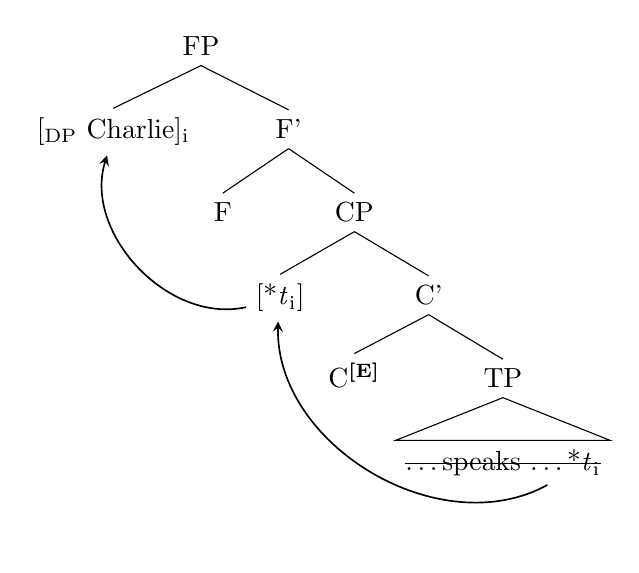
\begin{tikzpicture}[baseline]
   \tikzset{}
  \Tree[.FP \node(w){[\textsubscript{DP} Charlie]\textsubscript{i}}; [.F' F [.CP \node(i){[*\textit{t}\textsubscript{i}]}; [.C' C\textsuperscript{\textbf{[E]}} [.TP \edge[roof]; {\sout{\dots speaks \dots *\textit{t}\textsubscript{i}}} ] ] ] ] ];
\draw[semithick, -stealth] (i) to [bend left=60] (w);
 \draw[semithick, -stealth] (4.4,-5.45) to [bend left=60] (i);
\end{tikzpicture}

\caption{Derivation of a fragment answer to \ref{ex:merchant-abby-q} according to \citet[708]{merchant2004}.\label{fig:merchant-abby-a}}
\end{figure}
%
\citet[706]{merchant2004} accounts for this by assuming that traces\is{Trace (movement)} of movement across island\is{Island} boundaries have a feature *, which renders PF representations that contain such features uninterpretable. As \citeauthor{merchant2004} assumes that ellipsis is PF-deletion, it can delete such traces\is{Trace (movement)} at PF and thus ``repair'' the defective structure. \citeauthor{merchant2004} notes that his hypothesis can also account for the observation that sluicing\is{Sluicing} is not sensitive to island\is{Island}s but other ellipses, like VPE\is{Verb phrase ellipsis} and fragments, are. In sluicing\is{Sluicing}, the E feature\is{E feature} is located on C, so that it deletes all intermediate *\textit{t} traces\is{Trace (movement)} within the TP\is{Tense phrase} at PF. In contrast, movement in fragments\is{Movement and deletion account} targets [Spec, FP] and, by proceeding cyclically, it leaves a *\textit{t} in [Spec, CP\is{Complementizer phrase}], as the derivation of fragment answer to \Next in Figure \ref{fig:merchant-abby-a} shows. The trace in the specifier survives ellipsis and causes the derivation to crash, because E\is{E feature} is placed on C in fragments. 

\ex. Does Abby speak the same Balkan language that Ben speaks?\label{ex:merchant-abby-q}

In fact, the need to account for the island\is{Island} sensitivity of fragments is what motivates \citeauthor{merchant2004} to reject his initial assumption that E\is{E feature} is placed on F in fragments, which is illustrated in Figure \ref{ex:merchant.structure-reduced}. If this derivation was correct, the PF-deletion of the defective trace\is{Trace (movement)} would render fragments insensitive to island\is{Island}s, just like \citet{merchant2001} argues for sluicing\is{Sluicing}.
%
\begin{figure}
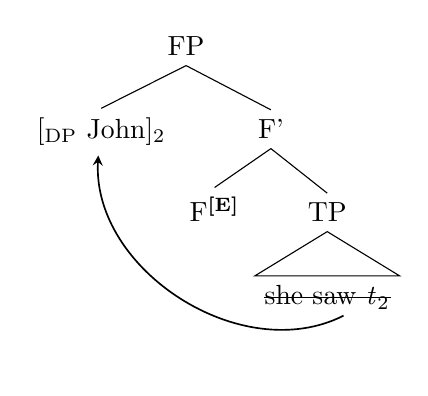
\begin{tikzpicture}[baseline]
   \tikzset{}
  \Tree[.FP \node(w){[\textsubscript{DP} John]\textsubscript{2}}; [.F' F\textsuperscript{\textbf{[E]}} [.TP \edge[roof]; {\sout{she saw \textit{t}\textsubscript{2}}} ] ] ];
\draw[semithick, -stealth] (2,-3.3) to [bend left=60] (w);
\end{tikzpicture}
 
\caption{Derivation of fragments without an intermediate CP according to \citet[675]{merchant2004}.\label{ex:merchant.structure-reduced}} 
\end{figure}
%
Repair effects complicate the use of parallelisms between fragments and sentences as a diagnostic for movement. As \citet[711]{merchant2004} puts it, ``[\dots] the general argument is that parallelisms support a movement and ellipsis analysis, while non-parallelisms reveal repair effects.'' Nevertheless, repair effects cannot just be stipulated but require an analysis, like the one involving the * feature on traces\is{Trace (movement)} that results from island\is{Island} violation.

\citepos{weir2014} exceptional movement\is{Exceptional movement account} account predicts an even larger set of mismatches between fragments and sentences than \citet{merchant2004} because exceptional movement\is{Exceptional movement account} occurs only in fragments and is therefore relatively independent from movement in sentences. \citeauthor{weir2014} only restricts exceptional movement\is{Exceptional movement account} to those movement operations that are ``in principle'' available in a language.  The derivation of empirically testable predictions for his account would require criteria that define which types of movement are available in principle and which are not, but \citet[10]{weir2015} offers no such criteria and instead proposes that it ``is most easily shown by example'' how a movement operation is to be classified. He exemplifies this reasoning with the impossibility of fronting NPIs \Next[a] and bare quantifiers \NNext[a] in English\is{English} (the judgments are Weir's) and argues that left dislocation of such expressions is not blocked due to a syntactic restriction because argument DPs\is{Determiner phrase} can be fronted in English\is{English} \ref{ex:weir-fronting}. Consequently, he attributes the ungrammaticality of \Next[a] and \NNext[a] to some kind of semantic ill-formedness and takes this to illustrate the PF-only character of exceptional movement\is{Exceptional movement account}.

\ex.What didn't John buy? \hfill \citep[adapted from][3]{weir2015}
\a. ??Any wine, John didn't buy \textit{t}.
\b. Any wine.

\ex. Who will you talk to? \hfill \citep[adapted from][3]{weir2015}
\a. *Someone, I will talk to \textit{t}.
\b. Someone.

\ex. That guy, I saw \textit{t}.  \hfill \citep[10]{weir2015} \label{ex:weir-fronting}

The absence of criteria for which types of movement are in principle available makes it almost impossible to empirically evaluate the exceptional movement\is{Exceptional movement account} account. However, what matters from an empirical perspective is that \citet[11]{weir2015} explicitly excludes P-stranding\is{Preposition stranding} \citep{pullum.huddleston2002}, and left-branch extraction \citep{ross1967, boskovic2005} in languages which do not allow for either of these operations from the set of movement operations that are available in principle. Therefore, languages which do not lack these phenomena but which will allow for the generation of the corresponding fragments would also provide evidence against exceptional movement.

Repair effects, and in particular exceptional movement\is{Exceptional movement account}, notably complicate the predictions of the movement and deletion\is{Movement and deletion account} account on the correlation between the acceptability of fragments and left dislocation. Specifically, some of the mismatches in acceptability between acceptable elliptical and nonelliptical structures would not provide evidence against movement and deletion\is{Movement and deletion account} if they can be explained by some kind of repair effect. Nevertheless, repair effects increase the complexity of the theory and therefore require independently motivated accounts that justify them. The assumption of defective traces\is{Trace (movement)} by \citet{merchant2004} discussed above might provide such an account, but it still requires independent empirical evidence, for instance, one showing that similar observations can be made for related phenomena. However, and in the first place, empirical perspective however, the movement and deletion\is{Movement and deletion account} account requires evidence \textit{for} movement in fragments\is{Movement and deletion account} that cannot be explained by other theories, like nonsentential approaches or the derivationally simpler in situ deletion\is{In situ deletion account} account.\is{Movement restriction|)}

\subsection{Summary}
In this section I have discussed different potential testing grounds which might allow for the empirical evaluation of the competing accounts of fragments. Their respective predictions are summarized in Table \ref{tab:predictions}. 

\begin{table}
  \begin{tabular}{p{2.2cm}p{1.5cm}p{1.3cm}p{2.2cm}p{2.5cm}}
\lsptoprule
 ~~ & \citet{merchant2004} & \citet{reich2007} & \citet{barton.progovac2005} & \citet{bergen.goodman2015}\\
\midrule
Structural case & ~\ding{51} & \ding{51} & \ding{55} & \ding{51} \\
 Non-constituents  & (\ding{55}) &  \ding{51} & \ding{55} & \ding{51} \\
  Focus\linebreak sensitivity & ~\ding{51} & \ding{51} & \ding{55} & \ding{55} \\
  Movement\linebreak restrictions & (\ding{51})  & \ding{55} & \ding{55} & \ding{55} \\
\lspbottomrule
 \end{tabular}
\caption{Overview of the empirical predictions the accounts of fragments make on the phenomena discussed in this section. The predictions of \citet{merchant2004} with respect to non-constituent fragments and effects of movement restrictions depend on further theory-internal assumptions. Non-constituent fragment is predicted ot be acceptable when multiple movement to the left periphery is possible, e.g. in Italian \citep{cinque1990, rizzi1997}. Under the exceptional movement version of the theory \citep{weir2014}, movement restriction effects are only expected for movement which is unavailable \textit{in principle} in a language.\label{tab:predictions}}
 \end{table}
%
With respect to the question of whether fragments involve unarticulated structure, case connectivity effects\is{Case connectivity}, specifically with respect to structural case\is{Structural case} marking in fragments, turn out to be the most promising testing ground. Sentential accounts predict strict case connectivity, whereas the nonsentential account\is{Nonsentential account} predicts that fragments cannot appear in structural case\is{Structural case} and will exhibit default case\is{Default case} morphology instead. As argued above, whether a specific case is structural case\is{Structural case} in a language or whether it is not might be controversial, but the alternative, focus sensitivity, is even more difficult to test. The nonsentential account\is{Nonsentential account} does not rely on the concept of focus, but makes similar predictions due to the necessity to retrieve deleted expressions from context. Furthermore, it is difficult to empirically elicit specific focus structures, because focus is mostly encoded prosodically in English and German \citep[see e.g.][1658--1660]{zimmermann.onea2011}.

Testing whether fragments are derived by movement and deletion\is{Movement and deletion account}, as claimed by \citet{merchant2004}, obviously requires the investigation of whether movement restrictions\is{Movement restriction} constrain the form of fragments: Restrictions on the form of fragments and left-dislocated expressions would provide evidence for movement and deletion\is{Movement and deletion account} and the corresponding mismatches evidence against it. As for the former, it must also be shown that the nonsentential or the in situ deletion\is{In situ deletion account} accounts cannot account for the data, while the possibility of repair effects must be considered in case of apparent non-parallelisms. My experiments investigating movement restrictions\is{Movement restriction} take the studies by \citet{merchant.etal2013} on preposition omission\is{Preposition omission} and complementizer omission\is{Complementizer omission} as a starting point. The first of these phenomena will also allow for conclusions on \citepos{weir2014} exceptional movement\is{Exceptional movement account} theory, which seems to have a greater empirical coverage than the original version of movement and deletion\is{Movement and deletion account}, but it is also harder to test because of the lack of clear criteria that would distinguish movement operations that can occur in fragments from those that cannot.

As for the assumption that fragments are inherently ungrammatical, I noted above that it is impossible to verify but that it still can be falsified by evidence for linguistic constraints on the form of fragments that cannot be reduced to being the result of game-theoretic\is{Game theory} reasoning, as \citet{bergen.goodman2015} suggest.

In the next chapter, I present a series of experiments that test some of the predictions of the competing theories of fragments which I discussed in this section. Currently there is no consensus on the appropriate syntactic analysis of fragments, and there has been no systematic and empirical investigation of the partially contrary predictions of the theories. My experiments will to some extent fill this gap. The experiments address two main questions that allow us to differentiate between the theories presented in this chapter: First, I test whether fragments are underlyingly sentential. Since the results support a sentential account, I  address the question of whether movement restrictions\is{Movement restriction} constrain the form of fragments at the case of preposition omission\is{Preposition omission}, complementizer omission\is{Complementizer omission} and multiple prefield\is{Prefield} constituents in German\is{German}. Furthermore, the results on the syntax of fragments inform my experiments on their usage in Chapter \ref{sec:chapter-infotheory-experiments}.
\chapter[Experiments on the syntax of fragments]{Experiments on the syntax of fragments} \label{sec:chapter-experiments-syntax} 

In this chapter I present 11 experiments that empirically evaluate the theories of fragments which I introduced in the preceding chapter.%
%
\footnote{Experiments \ref{exp:case}, \ref{exp:pstranding-german}, \ref{exp:pstranding-english}, \ref{exp:ccs-german} and \ref{exp:ccs-english} have been published in \citet{lemke2017}. The statistical analyses differ from those reported here, but the conclusions drawn from the data remain the same.}\afterfn%
%
The experiments address two main research questions: First, the experiments \ref{exp:case}--\ref{exp:scripts-rating-case} investigate whether fragments are underlyingly sentential or whether they are genuine nonsententials. Since the experiments provide evidence for unarticulated structure in fragments, the experiments \ref{exp:pstranding-german}--\ref{exp:mvb} test whether the generation of fragments obligatorily involves movement or whether fragments are the result of in situ deletion. 

The experiments contribute to the theoretical analysis of fragments, by providing further empirical data on the competing theories' predictions. The experiments on default case\is{Default case} and multiple prefield\is{Prefield} constituents are the first attempts to empirically investigate theoretical assumptions that are solely based on introspective data so far and the studies on preposition omission and complement clause\is{Complement clause} topicalization extend previous experimental research. Additionally, these experiments will settle the ground for the experiments on the usage of fragments in Chapter \ref{sec:chapter-infotheory-experiments}, which requires to determine \textit{which} fragments are grammatical. Since the account of fragment usage that I propose in Chapter \ref{sec:chapter-infotheory} presupposes that speakers choose between grammatical utterances, so its empirical predictions would be distorted by the inclusion of ungrammatical fragments in the set of utterances among which a speaker can choose. For instance, if fragments were subject to movement restrictions\is{Movement restriction}, as \citet{merchant2004} argues, only those expressions that can appear in a left-peripheral position would be possible fragments.

This chapter is structured as follows. Section \ref{sec:experiments-case} presents the experiments that test whether fragments are sentential (experiments \ref{exp:case}--\ref{exp:scripts-rating-case}). I use structural case marking on DP\is{Determiner phrase} fragments as a testing ground for this, because \citet{barton.progovac2005} argue that DP\is{Determiner phrase} fragments cannot appear in structural case. The experiments support a sentential account, since they show that, provided an appropriate context, structural case is preferred over default case\is{Default case} in fragments.

Sections \ref{sec:pstranding}--\ref{sec:mvb} present the experiments on three movement restrictions\is{Movement restriction}: Pre\-position omission (experiments \ref{exp:pstranding-german}--\ref{exp:pstranding-production}), complement clause\is{Complement clause} topicalization (experiments \ref{exp:ccs-german}, \ref{exp:ccs-english}) and multiple prefield\is{Prefield} configurations in German\il{German} (experiment \ref{exp:mvb}). In Section \ref{sec:pstranding}, I present four experiments that investigate whether restrictions on preposition stranding\is{Preposition stranding} constitute evidence for movement in fragments\is{Movement and deletion account}. The first two experiments support the pattern predicted by \citet{merchant2004} for English\il{English} and German\il{German}, and the latter experiments investigate potential non-movement accounts of this pattern: Experiment \ref{exp:pstranding-defaultcase} investigates a case checking\is{Case feature}-based approach to preposition omission in fragments by \citet{progovac.etal2006}, which is disconfirmed. Experiment \ref{exp:pstranding-production}, however, suggests that, based on English\il{English} data, a nonsyntactic relationship between question and answer can explain the data without necessarily assuming movement. Section \ref{sec:ccs} addresses complement clause\is{Complement clause} topicalization with two experiments. In part, these studies replicate the effect reported by \citet{merchant.etal2013} for fragments, but crucially not for the corresponding left dislocation structures. The data hence cannot be interpreted as evidence for movement. Finally, in Section \ref{sec:mvb} I test the predictions of the movement and deletion\is{Movement and deletion account} account on fragments that are derived from ungrammatical multiple prefield\is{Prefield} configurations in German\il{German} (experiment \ref{exp:mvb}). Again, the experiment does not reveal the pattern predicted by \citepos{merchant2004} theory. Section \ref{sec:syntax-gdiscussion} summarizes the main results of the experiments. 

\section{Case marking as evidence for sententiality}
\label{sec:experiments-case}

This section presents three experiments that test these predictions of sentential and nonsentential accounts\is{Nonsentential account} with respect to structural case marking. As I discussed in Section \ref{sec:theories-predictions-case}, all sentential accounts predict case connectivity effects\is{Case connectivity}: DP\is{Determiner phrase} fragments always receive the same case morphology as the corresponding DP within a full sentence, because the structure of the full sentence from which they are derived determines their case. In contrast, the nonsentential account by \citet{barton.progovac2005} predicts that fragments may not receive structural case marking: Unlike default\is{Default case} or inherent\is{Inherent case} case, structural case needs to be checked by a verbal or functional head, which they argue is not present in DP\is{Determiner phrase} fragments. Instead, they claim that DP\is{Determiner phrase} fragments that exhibit structural case in full sentences appear in default\is{Default case} case in fragments. The pattern is exemplified in \Next. \citet{barton.progovac2005} predict such anticonnectivity effects\is{Case connectivity} only for structural case-marked DP\is{Determiner phrase}s, because inherent\is{Inherent case} case, e.g. dative\is{Dative case} or genitive\is{Genitive case}, is interpretable and therefore does not require feature checking.\largerpage[-1]

\begin{table}
\begin{tabular}{l l l l l}
\lsptoprule
Case & masc, sg. & fem, sg. & neut, sg. & plural\\
\midrule
Nom & der Mann & die Frau & das Buch & die Männer/Frauen/Bücher\\
Gen & des Mannes & der Frau & des Buch(e)s & der Männer/Frauen/Bücher\\
Dat & dem Mann & der Frau & dem Buch & den Männer/Frauen/Bücher\\
Acc & den Mann & die Frau & das Buch &  die Männer/Frauen/Bücher\\
\lspbottomrule
\end{tabular}
\caption{German inflectional case paradigm for masculine, feminine and neuter definite DPs (\textit{the man}, \textit{the woman}, \textit{the book}).\label{tab:case-paradigm-german}}
\end{table}

\ex. Who can eat another piece of cake? \hfill \citep[77]{barton.progovac2005} 
\a. ?*I/?*We/?*He/?*She
\b. Me/Us/Him/Her

The case of pronouns is more complex than \citet{barton.progovac2005} suggest. The crosslinguistic data on the contrast between strong, weak and tonic pronouns in \citet{merchant2004} shows that not only case, but also information structure\is{Information structure} determines which form of a pronoun is selected. What is more, English\il{English} has only reduced morphological case marking, therefore it is not the ideal language for testing differences between default\is{Default case}, inherent\is{Inherent case} and structural case. For this reason, in experiments \ref{exp:case}--\ref{exp:scripts-rating-case} I investigate the phenomenon in German\il{German}, a language that has a richer case system than English\il{English}. In German\il{German} there are four cases, whose morphological realization on definite DPs\is{Determiner phrase} is exemplified in Table \ref{tab:case-paradigm-german}.

Case marking occurs most systematically on the article. There are some syncretic forms for plurals as well as for feminine and neuter singular DPs\is{Determiner phrase}, but for some masculine singular DPs\is{Determiner phrase} the determiner disambiguates fully between the four cases.%
%
\footnote{For other masculine singular DPs\is{Determiner phrase} only nominative\is{Nominative case} is morphologically distinct from the remaining cases, as \Next shows. See e.g. \citet[139--141]{eisenberg1999} for details.

\exg. der Student / des Studenten / dem Studenten /  den Studenten\\
      the.\textsc{nom} student.\textsc{nom} /  the.\textsc{gen} student.\textsc{gen} / the.\textsc{dat} student.\textsc{dat} /  the.\textsc{acc} student.\textsc{acc}\\


}\afterfn%
%
Dative\is{Dative case} and genitive\is{Genitive case} are inherent\is{Inherent case}, because they are related to specific thematic roles or selected by specific lexical items.%
%
\footnote{See also \citet{woolford2006}, who distinguishes between lexical case, that is selected by a lexical item and inherent\is{Inherent case} case, which encodes a specific \texttheta-role.}\afterfn%
% 
Given the discussion in the preceding section, accusative\is{Accusative case} must be analyzed as structural case, which marks the direct object of a verb. Nominative\is{Nominative case} marks the syntactic subject and is the default case\is{Default case} in German\il{German} (if such a concept is assumed at all).

\refstepcounter{expcounter}\label{exp:case}
\subsection{Experiment \ref{exp:case}: Default case, acceptability rating study} \label{sec:fragments-case-rating}


\subsubsection{Background}
\label{sec:fragments-case-background}

In experiment \ref{exp:case}, I investigate whether structural case connectivity effects\is{Case connectivity} occur in German\il{German}. I test this with an acceptability rating\is{Acceptability rating task} task that compares nominative\is{Nominative case} \Next[a] and accusative\is{Accusative case} \Next[b] DP\is{Determiner phrase} fragments. The nonsentential account\is{Nonsentential account} by \citet{barton.progovac2005} predicts that DP\is{Determiner phrase} fragments cannot appear in structural case so that accusative\is{Accusative case} DP\is{Determiner phrase} fragments would be degraded as compared to nominative\is{Nominative case} default case\is{Default case}. In contrast, sentential accounts predict case connectivity: If the DP\is{Determiner phrase} has accusative\is{Accusative case} case marking in the full sentence from which it is derived, accusative\is{Accusative case} is preferred over nominative\is{Nominative case}.

\ex. Jenny and David want to drive to the beach today. While David is packing the picnic basket, he says to Jenny:\exsourcelowered{Nominative}\label{ex:case-sample-item}
\ag. Der Sonnenschirm!\\ 
the.\textsc{nom} sun.shade\\
\bg. Den Sonnenschirm!\\
the.\textsc{acc} sun.shade\\
\trans{The sunshade!}\exsourceraised{Accusative}

\is{Context, extralinguistic|(}
The strength of connectivity effects\is{Case connectivity} expected under sentential accounts depends on the QuD\is{Question under Discussion} or context that is accommodated. For instance, in \Last, one could in principle assume either of the structures in \Next as underlying the fragment, but accusative\is{Accusative case} is only licensed in the case of \Next[a]. Therefore, if it was more natural to choose \Next[b] than \Next[a], sentential accounts would also predict a preference for nominative\is{Nominative case}, which however would be explained by connectivity effects\is{Case connectivity} and not by default case\is{Default case} morphology. In order to control the availability of structural case in a complete sentence, the fragments were preceded by a context story that made such a sentence salient. A pretest ensures that e.g. \Next[a] is accessible in this context. Furthermore, experiment \ref{exp:case-production} shows that accusative\is{Accusative case} is also more likely to be used in a production task\is{Production task}.\largerpage[-1]
 
\ex. 
\ag. Wir müssen noch den Sonnenschirm einpacken!\label{ex:case-acc-sentential}\\ 
we must still the.\textsc{acc} sun.shade pack.in\\
\trans{We still have to load the sunshade (in the car).}\exsourceraised{Accusative}
\bg. Der Sonnenschirm ist noch nicht im Auto!\\
the.\textsc{nom} sun.shade is yet not in.the car\\
\trans{The sunshade is not yet in the car!}\exsourceraised{Nominative}

\begin{table}
\begin{tabular}{lcc}
\lsptoprule
 & Nominative\is{Nominative case} & Accusative\is{Accusative case} \\
\midrule
Nonsentential account\is{Nonsentential account} & \phantom{(}\ding{51}\phantom{)} & \ding{55}\\
Sentential account\is{In situ deletion account}\is{Movement and deletion account} & (\ding{51}) & \ding{51}\\
Ungrammatical\is{Ungrammaticality of fragments} & (\ding{51}) & \ding{51}\\
\lspbottomrule
\end{tabular}
\caption{Predictions of the nonsentential and sentential accounts on the acceptability of case-marking in fragments.\label{tab:case-predictions}}
\end{table}

However, even if \Last[a] was more accessible than \Last[b], sentential accounts do not necessarily predict that nominative\is{Nominative case} is less acceptable than accusative\is{Accusative case} in an  acceptability rating\is{Acceptability rating task} task. Under the assumption of case connectivity\is{Case connectivity} the hearer must retrieve an antecedent that requires nominative\is{Nominative case} case marking after processing a nominative\is{Nominative case} case-marked fragment. In the event he is able to retrieve such an antecedent, nominative\is{Nominative case} might be perceived as acceptable as well. Table \ref{tab:case-predictions} summarizes the predictions of the two (families of) theories. Contexts in which a sentence requiring accusative\is{Accusative case} case marking is accessible allow us to distinguish between the predictions of both families of accounts: The  nonsentential account\is{Nonsentential account} predicts a strong preference for nominative\is{Nominative case}, but if a sentential account is correct, accusative\is{Accusative case} must be at least as acceptable as nominative\is{Nominative case}.
\is{Context, extralinguistic|)}

\subsubsection{Materials}
\label{sec:case-materials}
All materials follow the pattern in \Next and \NNext, that is, they consist of a DP\is{Determiner phrase} fragment preceded by a context story. The context story introduces two characters and a situation, at the end of which one of the two characters utters the fragment. The story ensures that a full sentence that requires accusative\is{Accusative case} case marking is accessible, as was confirmed by a pretest (see Section \ref{sec:case-pretest} below for details). All fragments are masculine singular DP\is{Determiner phrase}s and appear in one of two \textsc{Case} conditions (accusative\is{Accusative case}/nominative\is{Nominative case}). The restriction to masculine singular nouns excludes case-syncretic forms. Whenever this does not reduce naturalness, the DP\is{Determiner phrase}s contain an adjective, so that case marking appears twice and is more salient, as in \NNext. This is particularly important in the case of the accusative\is{Accusative case} indefinite article \textit{einen}, which is often pronounced as \textit{ein} in colloquial speech. I used only discourse-initial fragments\is{Fragment, discourse-initial} because, as discussed in the introduction (Section \ref{sec:intro-fragments}), some authors \citep[e.g.][]{klein1993, reich2011} distinguish short answers\is{Fragment, short answer}, which have a linguistic antecedent, from discourse-initial fragments\is{Fragment, discourse-initial}. Discourse-initial fragments definitely lack an overt linguistic antecedent, hence they are the most uncontroversial instances of fragments.

\ex. Jenny and David want to drive to the beach today. While David is packing the picnic basket, he says to Jenny: \exsourcelowered{Nominative}\is{Nominative case}
\ag. Der Sonnenschirm!\\ 
the.\textsc{nom} sun.shade\\
\bg. Den Sonnenschirm!\\
the.\textsc{acc} sun.shade\\
\trans{The sunshade!}\exsourceraised{Accusative}

\ex. Thomas sits at a table in the coffee shop and reads his newspaper. As the waiter approaches his table, Thomas says:\label{ex:fragments-item-xplease}
\ag. Ein doppelter Espresso.\\
a.\textsc{nom} double.\textsc{nom} espresso\\
\trans{A double espresso.} \exsourceraised{Nominative}
\bg. Einen doppelten Espresso.\\
a.\textsc{acc} double.\textsc{acc} espresso\\
\trans{A double espresso.} \exsourceraised{Accusative}

In some of the stimuli, e.g. \Last, the DP\is{Determiner phrase} fragment has the function of ordering something, like food in a restaurant. In his discussion of a similar example, \citet[731]{merchant2004} notes that in highly conventionalized scenarios ``quite complex syntactic structures can be conventionally elided [\dots]. This case, therefore, is somewhat special in not having precisely the same kind of underlying syntactic structure that other fragments do.'' Since \citeauthor{merchant2004} suggests that such conventionalized fragments might structurally differ from those used in non-conventionalized contexts, it is necessary to ensure that a potential preference for accusative\is{Accusative case} in the experiment is not driven by conventionalized fragments alone. Otherwise, the experiment would not allow for conclusions on the derivation of non-conventionalized fragments. For this reason, I tested only four out of 20 fragments that could be paraphrased by \textit{I would like an X, please!} or \textit{Would you like an X, please?}, X being an accusative\is{Accusative case}-marked semantically fitting DP\is{Determiner phrase}. Furthermore, the statistical analysis contained a control predictor \textsc{XPlease} in order to quantify and isolate potential effects of such conventionalized fragments.

\subsubsection{Pre-test}
\label{sec:case-pretest}

Before the main experiment, it was necessary to ensure that the structure that supposedly underlies the materials and that requires accusative\is{Accusative case} is easily accessible given the context story that preceded the fragment. If no corresponding full sentence that requires accusative\is{Accusative case} on the DP\is{Determiner phrase} was available, neither the sentential nor the nonsentential accounts\is{Nonsentential account} would predict accusative\is{Accusative case} case-marking. In that case, the experiment would not allow for a comparison of the theories' predictions. Therefore, I conducted a pretest in order to select 20 stimuli for the main experiment that made a sentence accessible that requires accusative\is{Accusative case}.

I constructed 40 items following the pattern in \ref{ex:case-sample-item}: Two context sentences introduced two characters and were followed by a target utterance attributed to one of these characters which seemed intuitively likely to be produced in this situation. In the pretest, the target utterance was always a complete sentence containing a transitive matrix verb and an accusative\is{Accusative case} case-marked DP\is{Determiner phrase} in its post-verbal base position \Next. This DP\is{Determiner phrase} was equivalent to the DP\is{Determiner phrase} fragment in the main experiment. Subjects were asked to rate the naturalness\is{Acceptability rating task} of the target utterance in the context of the story. In order to present not only (probably) accessible utterances throughout the pretest, a second context story was constructed for each of the target utterances, for which the target utterance was intuitively less accessible, yet not implausible. This yielded an additional unpredictive condition for which I expected worse ratings than for the predictive one. The context story for the unpredictive condition of the sample item \ref{ex:case-sample-item} is given in \NNext.\largerpage

\exg. Wir müssen noch den Sonnenschirm einpacken!\\ 
we must still the.\textsc{acc} sun.shade pack.in\\
\trans{We still have to load the sunshade (in the car).}

\ex. Jenny and David want to spend a relaxing day in their garden.\linebreak As Jenny walks outside with her book, David says:

Twenty-nine voluntary undergraduate students of Saarland University participated in the pretest, which was conducted over the Internet using the LimeSurvey questionnaire software \citep{limesurveygmbh2012}. Subjects were asked to rate the naturalness of the italicized target utterance in the context of the preceding story on a 7-point Likert scale (7 = completely natural). Materials were distributed across two lists so that each subject saw each token set once and only in one condition and each condition equally often. Each subject rated\is{Acceptability rating task} 40 items (20 in the predictive condition and 20 in the unpredictive one), which were mixed with 65 fillers and presented in individual fully randomized order. The fillers resembled the items in consisting of a two-sentence context story and a full sentence uttered by one of the two characters introduced in that story. Five of the fillers included utterances that were grammatically well-formed and not fully implausible, but intuitively unlikely in the described situation. Two participants who rated\is{Acceptability rating task} more than the previously established threshold of 50\% of these controls with 6 or 7 points were excluded from further analysis. Since the purpose of the pretest was to establish how accessible an utterance is in context, this ensured that only subjects whose ratings reflected this entered the analysis.

Across all items, utterances were rated\is{Acceptability rating task} as more natural in the predictive condition \descriptives{5.43}{1.8} than in the unpredictive one \descriptives{3.63}{2.13}. 
Except for one token set, the target utterance was always rated\is{Acceptability rating task} as more natural in the predictive condition than in the corresponding unpredictive one. An analysis with cumulative link mixed models (in what follows, CLMMs) using the \texttt{ordinal} package \citep{christensen2015} in \texttt{R} \citep{rcoreteam2019}%
%
\footnote{The analysis followed the procedure described for the main experiment in Section \ref{sec:intro-stats}.}\afterfn%
%
reveals a significant main effect of \textsc{Predictability} that evidences that target utterances are rated\is{Acceptability rating task} as significantly more natural in the predictive condition \clmmLR{40.37}{\highsig}. This shows that the intended predictability manipulation was successful. Based on the aggregated rating data by items, the 20 items that received the highest ratings in the predictive condition were selected as materials for the main experiment. The selected materials had a mean rating of 6.03 (range 5.54--6.5), whereas the discarded ones had a mean rating of 4.83 (range 3.0--5.46).

\subsubsection{Procedure (Main experiment)}
\label{sec:fragments-case-rating-method}
Seventy undergraduate students of Saarland University, Potsdam University and Stutt\-gart University%
%
\footnote{The reason for testing subjects from universities outside Saarbrücken was that dialects spoken in Saarbrücken and the surrounding areas exhibit case syncretism between accusative\is{Accusative case} and nominative\is{Nominative case} and could therefore be insensitive to this distinction. However, the statistical analysis showed that the behavior of subjects from the Saarbrücken region did not differ significantly from that of the subjects from regions without case syncretism.}\afterfn%
% 
participated in the experiment, which was conducted on the Internet via LimeSurvey. They were compensated with a lottery of 10 times \currencyEuro{30} among all participants. Subjects were asked to rate the naturalness of the target sentence, which was highlighted by italic font, on a 7-point Likert scale with labeled extremes (1 = very unnatural, 7 = very natural). Subjects were randomly assigned to one of four lists%
%
\footnote{As experiment \ref{exp:case} has two conditions, each two of the lists were equal with respect to the items from this experiment, but they differed in the items from experiment \ref{exp:pstranding-german} that were included.}\afterfn%
%
so that each subject saw each token set once and only in one condition. Each subject rated\is{Acceptability rating task} 20 items (10 per \textsc{Case} condition), which were presented together with 20 items from experiment \ref{exp:pstranding-german} and 47 fillers (including nine ungrammatical controls) in individually fully randomized order.  Fillers consisted of short stories or dialogues which contained direct speech by at least one of the characters in the story in order to resemble the materials. The target utterance was always a fragment. Among the fillers there were nine ungrammatical controls, which contained e.g. agreement violations or wrong verb inflections. No subject rated\is{Acceptability rating task} more than 50\% of the controls as acceptable (6 or 7 points on the scale), so that nobody was excluded from further analysis.

\subsubsection{Data analysis}
\label{sec:intro-stats}

I analyzed the data with cumulative link mixed models (CLMMs) \citep{christensen2015} in \texttt{R} \citep{rcoreteam2019}. CLMMs model the outcome of ordinal dependent variables and take into account the potentially differing distance between the scale items. Unlike linear models, they do not presuppose that the scale is unbound.%
%
\footnote{\citet[28]{gibson.etal2011} note that linear regression can still be used for ordinal data, unless the ratings are close to the endpoints of the scale. In fact, for most of the experiments reported in this book, linear mixed effects regressions conducted with the \texttt{lme4} package \citep{bates.etal2015} yield comparable results.}\afterfn%
%
This is implemented by threshold parameters that quantify this distance between scale items. The \texttt{ordinal} package allows for the modeling of these thresholds as flexible (individual thresholds for each transition between two categories), symmetric (different transitions between scale extremes and mid-range) and equidistant (same distance between all categories). I always started with the most complex structure (flexible thresholds) and subsequently shifted to simpler thresholds whenever this did not significantly worsen model fit, as evidenced by likelihood ratio tests calculated with the \texttt{anova} function in \texttt{R}.%
%
\footnote{For most of the analyses reported in this book, the final model had symmetric thresholds, as model fit was significantly worse with equidistant ones, but not significantly improved by additional parameters required for flexible thresholds. This evidences that subjects did not perceive the scale as linear, but that the difference between scale levels in the mid-range was not identical to that closer to the extremes.}\afterfn%
%

In order to determine the most appropriate model for the data, I used a backward model selection procedure. I started with a full model, which contains all predictors and two-way interactions between them and subsequently excluded effects that do not significantly improve model fit, as evidenced by likelihood ratio tests calculated with the \texttt{anova} function. Following \citet{barr.etal2013}, as long as models converged, I included the full random effects structure, i.e. by-subject and by-item random intercepts as well as by-subject and by-item random slopes for all predictors. $p$-values were calculated with likelihood ratio tests comparing the model fit of the final model to that of models without the specific predictor with the \texttt{anova} function in \texttt{R}. Besides explicitly stated differences, all statistical analysis reported in this work follow this procedure.

\subsubsection{Results}\label{sec:fragments-case-rating-results}

Figure \ref{fig:case-estimates} shows the mean acceptability ratings\is{Acceptability rating task} across the \textsc{Case} conditions and the \textsc{XPlease} variation between token sets. On average, accusative\is{Accusative case} fragments \descriptives{4.26}{2.09} were rated\is{Acceptability rating task} as more acceptable than nominative\is{Nominative case} fragments \descriptives{3.64}{2.08}. Fragments that could be paraphrased by a \textsc{XPlease} construction described above ($n = 4$) were rated\is{Acceptability rating task} as more acceptable \descriptives{5.16}{1.77} than those that could not \descriptives{3.65}{2.07}. The mean ratings suggest that the preference for accusative\is{Accusative case} is independent from the possible \textsc{XPlease} construction.

\begin{figure}
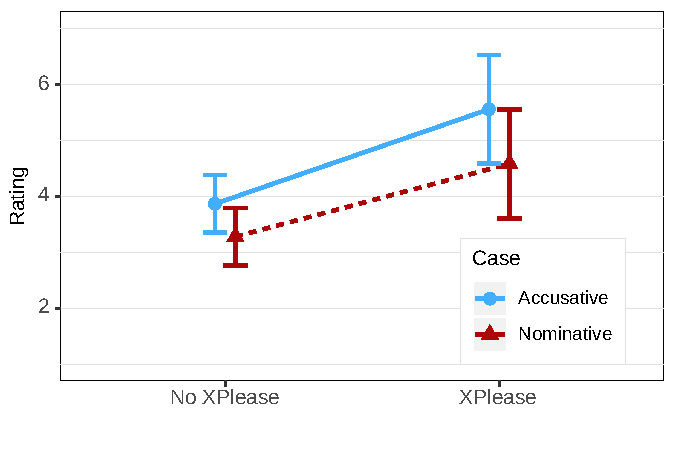
\includegraphics[width=10cm]{figures/ex1_case_estimates}
 \caption{Mean ratings and 95\% confidence intervals across conditions in experiment \ref{exp:case}. \label{fig:case-estimates}}
\end{figure}

I analyzed the data with CLMMs as described in Section \ref{sec:intro-stats}. The full model contained fixed effects for \textsc{Case} (binary), \textsc{XPlease} (binary) and the \textsc{Position} of the trial in the time-course of the experiment (numeric). The model included by-subject and by-item random intercepts and by-subject random slopes for \textsc{Case}, \textsc{XPlease} and their interaction. For items, I included only random slopes for \textsc{Case}, as \textsc{XPlease} was not varied systematically across token sets. The only fixed effects in the final model were those for \textsc{Case} and \textsc{XPlease} (see Table \ref{tab:case-estimates}): The main effect for \textsc{Case} shows that nominative\is{Nominative case} fragments were rated\is{Acceptability rating task} significantly as worse than accusative\is{Accusative case} fragments \clmmLR{7.39}{0.01}. The \textsc{XPlease} effect shows that fragments that could be paraphrased with an \textsc{XPlease} construction were significantly more acceptable than the others \clmmLR{7.3}{0.01}. There was no significant interaction between both predictors.

\begin{table}
\begin{tabular}{lccccc}
\lsptoprule
Predictor & Estimate & SE & $\chi^2$ &  $p$ &  \\   
\midrule
\textsc{Case} & -0.828 &  0.286 &7.39 & \textless 0.01 & ** \\
\textsc{XPlease} &    \phantom{-}1.875 &     0.632 &   7.30 &  \textless 0.01 & **\\
\lspbottomrule
\end{tabular}
\caption{Fixed effects in the final CLMM for experiment \ref{exp:case}. \label{tab:case-estimates}}
\end{table}

\subsubsection{Discussion}
Experiment \ref{exp:case} investigated case connectivity effects\is{Case connectivity} in German\il{German} accusative\is{Accusative case} DP\is{Determiner phrase} fragments, which would indicate unarticulated structure in fragments and hence provide evidence for a sentential theory of fragments. The data suggest that structural (accusative\is{Accusative case}) case marking is possible in fragments. Even in the absence of an explicit linguistic antecedent, accusative\is{Accusative case} DP\is{Determiner phrase}s are rated\is{Acceptability rating task} at least as acceptable as nominative\is{Nominative case} ones. In fact, the significant main effect of \textsc{Case} shows that accusative\is{Accusative case} is rated\is{Acceptability rating task} even better than nominative\is{Nominative case} if a full sentence requiring accusative\is{Accusative case} is accessible in context. This pattern is unexpected under the nonsentential account\is{Nonsentential account}, according to which accusative\is{Accusative case} is ungrammatical, but predicted by sentential accounts. From a sentential perspective, the acceptability of accusative\is{Accusative case} is analyzed as a case connectivity effect: Accusative case marking on the DP\is{Determiner phrase} is also required in the sentential alternative to the fragment, whose salience the pretest confirmed. If the data are to be explained by case connectivity\is{Case connectivity}, the lower ratings for nominative\is{Nominative case} indicate that a sentence that requires nominative\is{Nominative case} is unavailable, or at least less accessible in the case of my materials. 

This assumption has not been tested in the pretest, though. Even if the full sentence that requires accusative\is{Accusative case} was rated\is{Acceptability rating task} as perfectly natural in the pretest, this does not exclude the possibility that there is an equally accessible sentence that requires nominative\is{Nominative case}. In such a situation, the sentential account would predict no difference in acceptability between accusative\is{Accusative case} and nominative\is{Nominative case} fragments for my materials: No matter in which case the fragment appears, an antecedent for ellipsis resolution is accessible. If this was the case, the preference for accusative\is{Accusative case} in experiment \ref{exp:case} would still challenge the nonsentential account\is{Nonsentential account}, but neither would be in line with the case connectivity\is{Case connectivity} explanation that would provide evidence for sentential accounts of fragments. I address this issue with experiment \ref{exp:case-production}.

The \textsc{XPlease} predictor ensures that the overall preference for accusative\is{Accusative case} is not driven by only a few influential data points that might result from a conventionalized usage of accusative\is{Accusative case} fragments in contexts of ordering. In fact, the significant main effect of \textsc{XPlease} shows that these items are perceived as more acceptable than the remaining fragments. However, they were rated\is{Acceptability rating task} better in both \textsc{Case} conditions, and the absence of an interaction between \textsc{XPlease} and \textsc{Case} evidences that the preference for accusative\is{Accusative case} is independent of this construction. Possibly, in the potential \textsc{XPlease} construction the QuD\is{Question under Discussion} was easier to figure out or it is socially more appropriate to communicate with a fragment in such situations.

Table \ref{tab:ex-case-theories} summarizes different fragment theories' predictions on structural case-marking. If accusative\is{Accusative case} is structural case\is{Structural case} in German\il{German}, i.e. a purely linguistic device marking a structural relationship between the verb and its complement, the preference for accusative\is{Accusative case} clearly supports a sentential analysis. This holds even in the absence of explicit linguistic context\is{Context, linguistic}. Consequently, it is not an option to claim that short answers\is{Fragment, short answer} are elliptical and thus exhibit connectivity effects\is{Case connectivity}, while discourse-initial fragments\is{Fragment, discourse-initial} are genuine nonsententials and do not. %

\begin{table}
\begin{tabular}{lcc}
\lsptoprule
 & Nominative\is{Nominative case} & Accusative\is{Accusative case} \\
\midrule
Nonsentential account\is{Nonsentential account} & \phantom{(}\ding{51}\phantom{)} & \ding{55}\\
Sentential account\is{In situ deletion account}\is{Movement and deletion account} & (\ding{51}) & \ding{51}\\
Ungrammatical\is{Ungrammaticality of fragments} & (\ding{51}) & \ding{51}\\
\hline
Experiment \ref{exp:case} & \phantom{(}\ding{55}\phantom{)} &\ding{51} \\
\lspbottomrule

\end{tabular}
\caption{Summary of the predictions of fragment theories on structural case marking. \label{tab:ex-case-theories}}
\end{table}

Of course, the conclusion that the data challenge the nonsentential account\is{Nonsentential account} relies strongly on the theoretical distinction between structural, default\is{Default case} and inherent\is{Inherent case} case assumed by \citet{barton.progovac2005}: If accusative\is{Accusative case} was analyzed as inherent\is{Inherent case} case, the data would not conflict with the nonsentential account\is{Nonsentential account}. However, in Section \ref{sec:theories-predictions-case} I showed that the diagnostics presented by \citet{progovac.etal2006} as evidence that the Serbian\il{Bosnian/Croatian/Serbian} accusative\is{Accusative case} is indeed inherent\is{Inherent case} case yield the opposite result for German\il{German}.

So far, the data are in line with \citepos{bergen.goodman2015} view that fragments are per se ungrammatical but can be used as long as it is relatively easy to retrieve the omitted material. Any cue that guides the hearer toward the intended meaning will be useful for this purpose, and accusative\is{Accusative case} is definitely such a cue, because parsing the accusative\is{Accusative case} DP\is{Determiner phrase} rules out all possible meanings that require it to appear in a different case. Furthermore, as \citet{progovac.etal2006} note, accusative\is{Accusative case} DP\is{Determiner phrase}s will be relatively likely to be assigned the patient \texttheta-role. Furthermore, any case functions as a cue toward the associated \texttheta-role to some extent, as even the relatively unmarked nominative\is{Nominative case} reduces the likelihood of the DP\is{Determiner phrase} being a recipient (which usually receives dative\is{Dative case} case marking). However, this reasoning cannot reconcile the data with the nonsentential account\is{Nonsentential account} by \citet{barton.progovac2005}, who emphasize the categorical distinction between default\is{Default case}, inherent\is{Inherent case} and structural case.

\refstepcounter{expcounter}\label{exp:case-production}
\subsection{Experiment \ref{exp:case-production}: Default case, production study}
\label{sec:fragments-case-followup}
\subsubsection{Motivation}

Experiment \ref{exp:case-production} tested whether a sentential alternative that requires accusative\is{Accusative case} is indeed more salient in the context of the materials tested in experiment \ref{exp:case} than one that requires nominative\is{Nominative case}. Only in that case, the preference for accusative\is{Accusative case} in experiment \ref{exp:case} can be attributed to case connectivity\is{Case connectivity} and hence be interpreted as evidence for a sentential theory of fragments.

From a sentential perspective, the preference for accusative\is{Accusative case} in experiment \ref{exp:case} is explained by the availability of a linguistic antecedent for ellipsis which contains a verbal node licensing accusative\is{Accusative case} case marking on the fragment DP\is{Determiner phrase}. The salience of such an antecedent is confirmed by the high naturalness of sentential alternatives to the DP\is{Determiner phrase} fragments evidenced in the pretest. This line of reasoning, however, implies that a sentence that requires nominative\is{Nominative case} on the DP\is{Determiner phrase} is less accessible, because nominative\is{Nominative case} was perceived as less acceptable in experiment \ref{exp:case}. Since the pretest investigated only sentences containing accusative\is{Accusative case} DP\is{Determiner phrase}s, it is still possible that a sentence requiring nominative\is{Nominative case} is equally likely and the acceptability ratings\is{Acceptability rating task} call for a different explanation. Experiment \ref{exp:case-production} addresses this issue with a production study\is{Production task} using the same materials as experiment \ref{exp:case}. In contrast to the rating study, subjects produced the target utterance themselves. I then quantified the preference for full sentences that required accusative\is{Accusative case} or nominative\is{Nominative case} case marking on the fragment based on the aggregated responses.

\subsubsection{Materials}
The context stories of experiment \ref{exp:case} were used as stimuli in a production task\is{Production task}. Instead of reading a fragment, as in experiment \ref{exp:case}, subjects saw a hand-drawn image of the object referred to by the DP\is{Determiner phrase} fragment (see Figure \ref{fig:production-stim} for an example). Subjects were asked to read the story and to produce an utterance by the specified character that referred to the depicted object. The use of graphical stimuli avoided the problem that some (but not all) of the nouns in the DP\is{Determiner phrase} fragments tested in experiment \ref{exp:case} morphologically distinguish accusative\is{Accusative case} and nominative\is{Nominative case}, so that a written presentation would have introduced a case bias.

\begin{figure}
 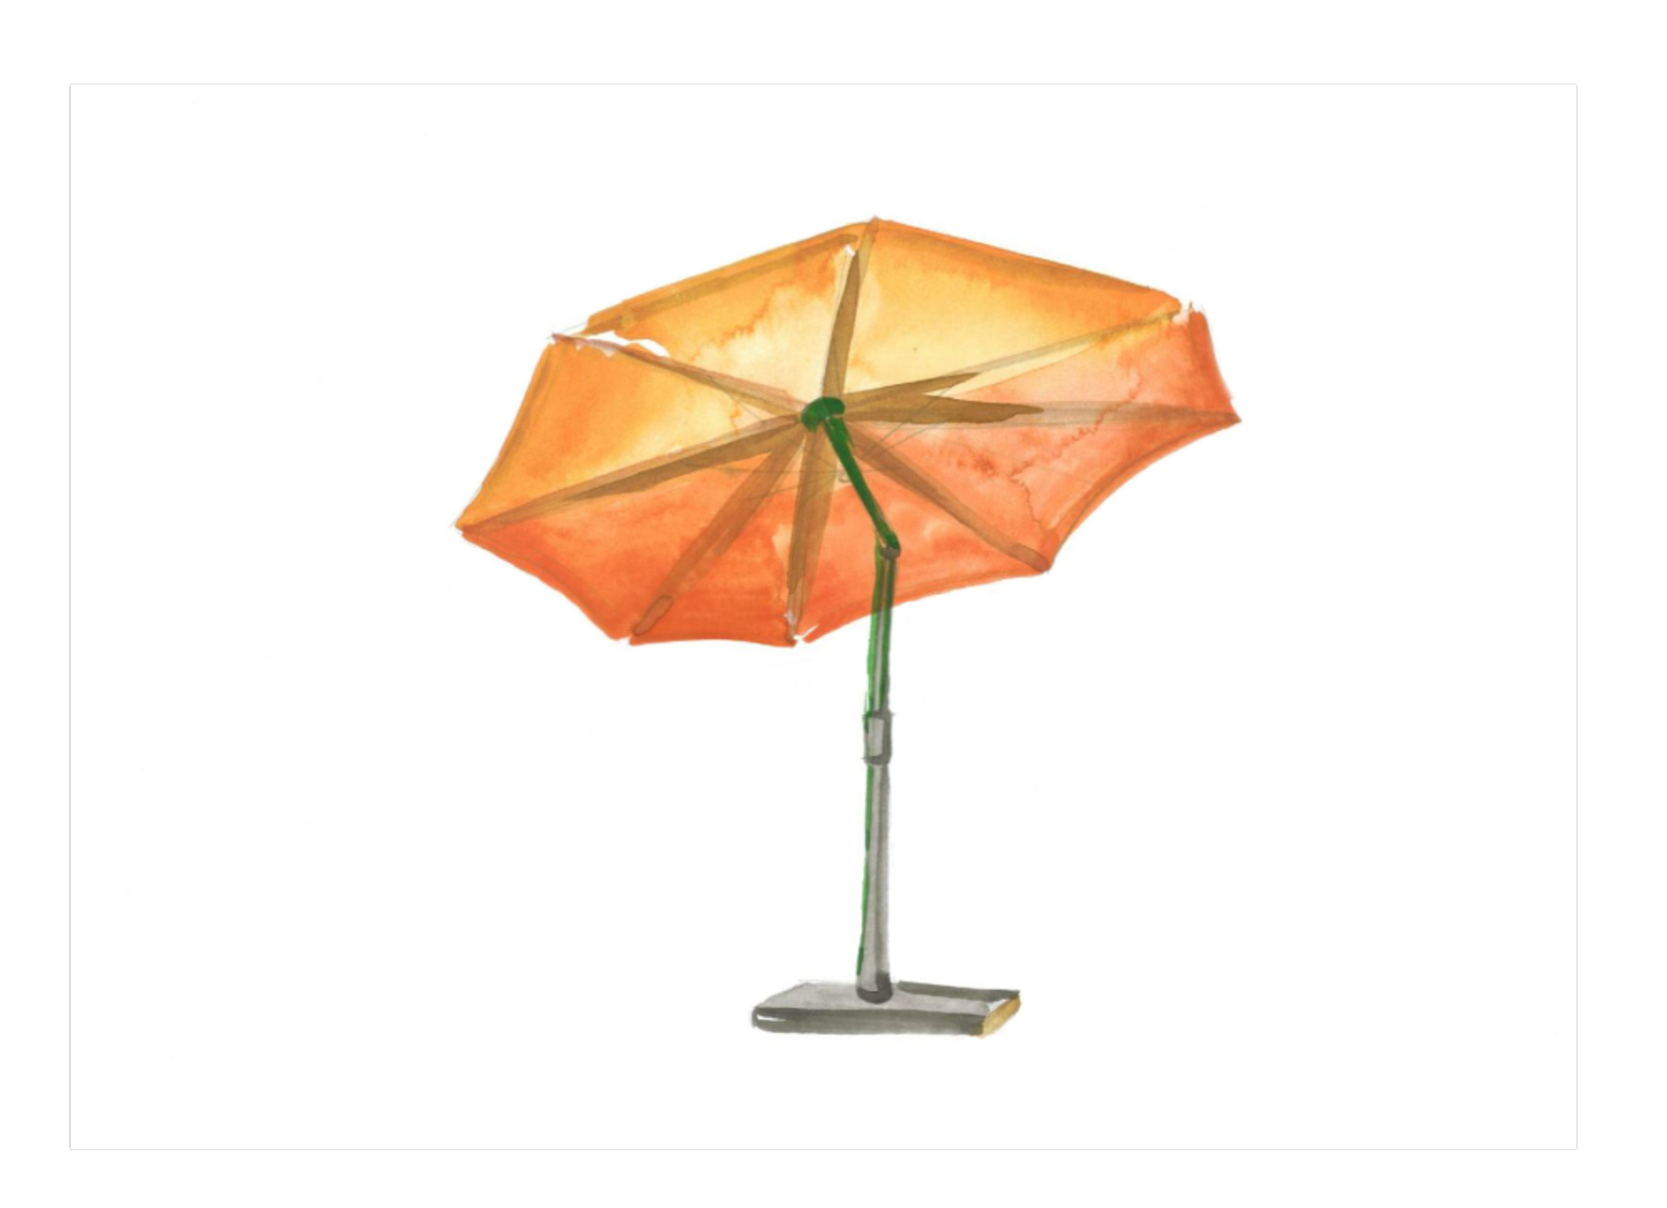
\includegraphics[scale=.3]{figures/production_sunshade.pdf}
 \caption{Sample graphical stimulus used in experiment \ref{exp:case-production} (CC-BY 4.0 Julia Stark).\label{fig:production-stim}}
\end{figure}

\subsubsection{Procedure}
The experiment was conducted over the Internet using the LimeSurvey survey presentation software and completed by 38 undergraduate students of Saarland University. They were rewarded with the participation in a lottery of 5 $\times$ \currencyEuro{30} among all participants. Subjects read the context story, which was presented above a hand-drawn image that depicted the object referred to by the corresponding DP\is{Determiner phrase} fragment in experiment \ref{exp:case}. They were asked to enter an utterance that was likely to be said by a specified character and that referred to the depicted object into a text field. As there was only one condition, all subjects saw the same materials. The experiment was presented to the same subjects as the acceptability rating\is{Acceptability rating task} study for \ref{exp:mvb} and the follow-up to experiment \ref{exp:ccs-german}. As the context stories contained no specifically biasing patterns that might prime subjects, there were no fillers, so that each subject produced 20 responses. The stimuli were presented in individually fully randomized order. The responses were manually annotated for the \textsc{Case} of the DP\is{Determiner phrase} referring to the image and the noun used in the DP\is{Determiner phrase} by the subjects. It was also annotated whether the subjects used the same lemma as tested in experiment \ref{exp:case}, a synonym, or whether they did not mention the lemma or a synonym at all. Responses that did not refer to the object depicted by the image (14.96\% of the data) were excluded from further analysis.

\subsubsection{Results}\largerpage[1.75]
There was a strong overall preference for accusative\is{Accusative case} (88.78\% of all trials) over nominative\is{Nominative case} (5.03\% of trials). The remaining 6.19\% of trials used other constructions that contained a DP\is{Determiner phrase} in dative\is{Dative case} or prepositional case\is{Prepositional case}.%
%
\footnote{In this context, prepositional case\is{Prepositional case} was always dative\is{Dative case} or accusative\is{Accusative case}. I distinguish prepositional case\is{Prepositional case} from other uses of dative\is{Dative case} and accusative\is{Accusative case} because e.g. \citet{zwarts2005} shows that prepositional case\is{Prepositional case} is in part determined by the preposition and not related to structure (accusative\is{Accusative case}) or a \texttheta-role (dative\is{Dative case}).}\afterfn%
%
The noun lemma produced by the subjects was the same as tested in experiment \ref{exp:case} in 49.7\% of the trials, a synonymous one in another 38.4\% and a closely related one (e.g. \textit{salad} instead of \textit{pasta salad}) in 11.9\% of the trials.

\begin{table}
\begin{tabular}{lccccc}
\lsptoprule
Predictor & Estimate & SE & $\chi^2$ &  $p$ &  \\   
\midrule
Intercept & -2.657 & 0.245 & 37.58 & \textless \highsig & *** \\
\lspbottomrule
\end{tabular}
\caption{Fixed effects in the final GLM for experiment \ref{exp:case-production}. \label{tab:case-production-estimates}}
\end{table}

Since the purpose of the experiment was to investigate the relative likelihood of accusative\is{Accusative case} and nominative\is{Nominative case} when referring to the target DP\is{Determiner phrase} and there were no predictors, I analyzed the data with an intercept-only logistic regression conducted with the \texttt{lme4} \citep{bates.etal2015} package in \texttt{R} \citep{rcoreteam2019}. The intercept of such a model indicates the likelihood of an observation to fall into one of the two categories, so that a significant intercept will show that these categories are not equally likely. The model in Table \ref{tab:case-production-estimates} shows that this is the case \glmer{37.58}{\highsig}. 

\subsubsection{Discussion}
Experiment \ref{exp:case-production} investigated whether a full sentence that requires accusative\is{Accusative case} case marking on the DP\is{Determiner phrase} fragment is indeed more likely than a sentence requiring nominative\is{Nominative case}. If this was the case, the pattern found in experiment \ref{exp:case} would indicate case connectivity\is{Case connectivity} and support a sentential theory of fragments. The production study\is{Production task} shows that accusative\is{Accusative case} was used significantly more often than nominative\is{Nominative case} in order to name the object referred to by the DP\is{Determiner phrase} fragment in experiment \ref{exp:case}. This is expected if the preference for accusative\is{Accusative case} or nominative\is{Nominative case} in experiment \ref{exp:case} is due to case connectivity\is{Case connectivity}: Accusative is preferred, because a full sentence that requires accusative\is{Accusative case} is the most salient antecedent for ellipsis that is made available through the context story. Taken together, experiments \ref{exp:case} and \ref{exp:case-production} provide clear evidence for unarticulated structure in fragments. First, fragments \textit{can} exhibit structural case morphology, and second, they \textit{do so} preferably when a fully sentential structure requiring structural case is salient in context.

\refstepcounter{expcounter}\label{exp:scripts-rating-case}
\subsection{Experiment \ref{exp:scripts-rating-case}: Mixed accounts?}  \label{sec:scripts-rating-case}
\subsubsection{Background}
\is{Mixed account|(}

Experiments \ref{exp:case} and \ref{exp:case-production} show that in contexts where a DP\is{Determiner phrase} appears in accusative\is{Accusative case} (structural case) in full sentences in German\il{German}, accusative\is{Accusative case} DP\is{Determiner phrase} fragments are also preferred over nominative\is{Nominative case} (default case\is{Default case}) DP\is{Determiner phrase} fragments. This finding is unexpected under the nonsentential account\is{Nonsentential account} by \citet{barton.progovac2005}, but it indicates case connectivity effects\is{Case connectivity}, which sentential accounts predict.

This result does not imply that \textit{all} fragments are generated by ellipsis. \citet{barton2006} raises the possibility of a \textit{mixed} account\is{Mixed account} of fragments, which derives some fragments  by ellipsis, whereas others are genuine nonsententials. Such an account would be motivated by the observation that the properties of fragments cannot be captured by a single syntactic mechanism alone. For instance, there might be both instances of case connectivity\is{Case connectivity} and anticonnectivity\is{Case connectivity}, so that both the nonsentential\is{Nonsentential account} and a sentential derivation would have to be assumed.

From a theoretical perspective, even that a mixed account\is{Mixed account} might account for the relevant data, Occam's Razor requires us to adopt one of the simpler accounts, unless a mixed captures the empirical picture better. To my knowledge, few serious attempts have been made to work out a mixed account\is{Mixed account} of fragments in detail. \citet{barton2006} cites \citet{morgan1989} and herself \citep{barton1998} as mixed account\is{Mixed account}s, but notes considerable differences between both with respect to the scope attributed to the sentential and nonsentential\is{Nonsentential account} generation mechanisms\is{Nonsentential account}. According to \citet{barton2006}, \citeauthor{morgan1989} adopts the nonsentential analysis\is{Nonsentential account} only for fragments that (arguably) cannot be explained by the sentential accounts, such as case-less Korean \il{Korean} DPs\is{Determiner phrase}, whereas \citet{barton1998} analyzes only those fragments that cannot be derived as genuine nonsententials as elliptical sentences. 

No matter how many of the empirically observed fragments are attributed to either derivation mechanism, spelling out a mixed account\is{Mixed account} necessarily involves explaining why the (non)sentential derivation is (not) available or (dis)\-preferred in a specific context. A straightforward implementation of a mixed account\is{Mixed account} could assume that a trade-off between the effort\is{Processing effort} required to find an antecedent that licenses ellipsis and a cost for pragmatic enrichment \citep{sperber.wilson1986, sperber.wilson1995,breheny.etal2006,  chevallier.etal2008} determines whether ellipsis resolution or pragmatic enrichment is used in order to interpret a fragment.%
%
\footnote{This is obviously the perspective of the hearer. However, since I assume that the speaker performs audience design\is{Audience design} \citep{bell1984}, the speaker will adapt her utterance to expectations about the interpretive behavior of the hearer.}\afterfn%
%
If pragmatic inference is effortful\is{Processing effort}, syntactic ellipsis resolution will be preferred when it is easy to retrieve an antecedent. The more difficult this retrieval becomes, the more promising might be the nonsentential derivation\is{Nonsentential account} that requires pragmatic inference by the hearer. A mixed account\is{Mixed account} based on this idea predicts case connectivity\is{Case connectivity} if there is a salient antecedent for ellipsis resolution and the generation of genuine nonsententials in case no salient antecedent is available.\largerpage%
%
\footnote{The mixed account\is{Mixed account} would obviously have to explain why a fragment is used at all if there is no salient antecedent that guides toward the meaning intended by the speaker.}\afterfn%
%

In experiment \ref{exp:case} I investigated only fragments that have a salient antecedent. Since the mixed account\is{Mixed account} predicts that such fragments are better resolved by ellipsis, it agrees with the sentential account in this case. However, if no salient antecedent is available, the mixed account\is{Mixed account} predicts that fragments are generated as nonsententials\is{Nonsentential account}. If genuine nonsentential utterances do not exhibit case connectivity\is{Case connectivity}, the predictions of sentential and nonsentential accounts diverge here: Sentential accounts predict strict case connectivity\is{Case connectivity}, and under the mixed account\is{Mixed account} sketched above structural case should be unavailable.

\begin{table}
\begin{tabular}{l c c c c}
\lsptoprule
 & \multicolumn{2}{c}{Predictable} & \multicolumn{2}{c}{Unpredictable} \\
 & Nom. & Acc.& Nom. & Acc.\\
\midrule
Nonsentential account &\ding{51} & \ding{55} & \ding{51} & \ding{55}\\
Sentential account & (\ding{51}) & \ding{51} & (\ding{51}) & \ding{51}\\
Mixed account & (\ding{51}) &\ding{51} & \ding{51} & \ding{55} \\
\lspbottomrule
\end{tabular}
 
\caption{Summary of the predictions of the nonsentential, sentential and mixed account with respect to experiment \ref{exp:scripts-rating-case}. \label{tab:scripts-case-theories}}
\end{table}

In experiment \ref{exp:scripts-rating-case} I therefore compared the acceptability\is{Acceptability rating task} of accusative\is{Accusative case} and nominative\is{Nominative case} fragments in predictable and unpredictable contexts in a 2$\times$2 design crossing \textsc{Predictability} and \textsc{Case} in an acceptability rating study\is{Acceptability rating task}. The predictions of the sentential, nonsentential\is{Nonsentential account} and mixed account\is{Mixed account} are summarized in Table \ref{tab:scripts-case-theories}. The nonsentential accounts\is{Nonsentential account} again predicts that accusative\is{Accusative case} is ungrammatical and that nominative\is{Nominative case} default case\is{Default case} is preferred. The sentential account predicts case connectivity\is{Case connectivity}: If there is a salient full sentence that requires accusative\is{Accusative case}, accusative\is{Accusative case} will be preferred. Finally, the mixed account\is{Mixed account} matches the behavior of the nonsentential account\is{Nonsentential account} for unpredictable fragments and that of the sentential account for predictable fragments. Fragments can be generated by ellipsis in predictive contexts, but are genuine nonsententials if no salient antecedent is available. 

\is{Mixed account|)}

\subsubsection{Materials}
The materials were derived from those used in experiment \ref{exp:scripts-rating} (see Section \ref{sec:scripts-rating}).The predictability of fragments was manipulated with context stories\is{Context, extralinguistic} based on event chains\is{Event chain} derived from the DeScript \citep{wanzare.etal2016} corpus\is{Corpus} of script knowledge\is{Script knowledge}.%
%
\footnote{In experiment \ref{exp:scripts-rating} some DPs\is{Determiner phrase} were ambiguous between accusative\is{Accusative case} and nominative\is{Nominative case} case. I replaced these DPs\is{Determiner phrase} by a semantically similar masculine singular noun that distinguishes accusative\is{Accusative case} and nominative\is{Nominative case} or chose a different event sequence from the same script.}\afterfn%
%
This ensures that the \textsc{Predictability} manipulation is founded on empirically observed event probabilities. In very simplified terms, the corpus\is{Corpus} allows for the estimation of the likelihood of an event in a script-based scenario given the previous events. For instance, a person who is cooking pasta will be likely to pour the pasta into the pot after the water is boiling. Under the assumption that likely events are more likely to be talked about than unlikely ones,%
%
\footnote{See Sections \ref{sec:scripts-rating-discussion} and \ref{sec:scripts-production-background} for a discussion.}\afterfn%
%
the likelihood of utterances in context can be quantified and manipulated based on the corpus\is{Corpus} data (see Section \ref{sec:infotheory-script-event-chains} for details). The stimuli consisted of short context stories of three sentences each and a fragment uttered by one of the characters introduced in the story \Next. The fragments were DPs\is{Determiner phrase} that referred to an event that was either predictable \Next[a,b] or unpredictable \Next[c,d] given the corpus\is{Corpus} data. 

\ex. Today, Marie and Jonas want to cook themselves a large serving of pasta with tomato sauce. As soon as the water started to boil, Jonas has added the pasta. After ten minutes, he says to Marie:
\ag. Der Topf mit den Nudeln.\\
     the.\textsc{nom} pot with the.\textsc{acc} pasta\\ 
     \exsourcefrombelow{Predictable, nominative}
\bg. Den Topf mit den Nudeln.\\
     the.\textsc{acc} pot with the.\textsc{acc} pasta\\
     \trans{The pot with the pasta.}  \exsourceraised{Predictable, accusative}
\cg. Der Küchentisch.\\
     the.\textsc{nom} kitchen.table\\ \exsourcefrombelow{Unpredictable, nominative}
\dg. Den Küchentisch.\\
     the.\textsc{acc} kitchen.table\\
     \trans{The kitchen table.} \exsourceraised{Unpredictable, accusative}

In both cases, in the corresponding full sentence \Next with default word order\is{Word order} the fragment appears in a post-verbal position and exhibits accusative\is{Accusative case} case morphology. In the predictable condition, the underlying sentence \Next[a] refers to the most likely event to follow the sequence of events underlying the context story, which is \textit{remove the pot from the stove} in the example. The context story refers to the events\is{Event chain} \textit{water starts to boil}, \textit{add pasta to the water} and \textit{cook pasta}. In the unpredictable condition, the event that the target utterance \Next[b] referred to (\textit{set table}) was not mentioned in the corpus\is{Corpus} data, but it is intuitively not fully implausible.     
     
\ex. \ag. Nimm  den Topf mit den Nudeln vom Herd.\\
	  take.\textsc{imp} the.\textsc{acc} pot with the.\textsc{acc} pasta off-the.\textsc{dat} stove\\
	  \trans{Take the pot with the pasta off the stove.}
     \bg. Deck doch schonmal den Küchentisch.\\
	  set.\textsc{imp} \textsc{prt} already the.\textsc{acc} kitchen.table\\
	  \trans{Set the kitchen table, please.}

In principle, it would have been desirable to keep the target utterance as constant as possible across conditions and to vary only those properties that are related to the variables that are investigated by presenting a single fragment in an unpredictive and a predictive context. However, if an unpredictive context for the fragment in \LLast[a] that is not based on the corpus\is{Corpus} data had been constructed from scratch, it would have been impossible to quantify the likelihood of the \textit{remove pot} event in the same fashion as in the predictable condition. This likelihood could also be measured in a norming study, but this would have required considerably more effort than relying on the corpus\is{Corpus}-based probabilities that were available from experiment \ref{exp:scripts-rating}. Alternatively, the fragment could have been presented with a different corpus\is{Corpus}-based context story for which it is known that the corresponding event does not happen (e.g. describing the train ride scenario) in the unpredictable condition. In this case though, the target utterance would not only be unlikely, but actually implausible and therefore probably highly degraded in any \textsc{Case} condition.

\subsubsection{Procedure}
The experiment, which was conducted on the Internet via LimeSurvey, was completed by 47 native speakers of German\il{German}, who were recruited through the crowdsourcing platform \textit{clickworker}. Subjects were paid \currencyEuro{4} for participating in the study. They were asked to rate the naturalness of the italicized target utterance in the context of the story on a 7-point Likert scale (7 = fully natural). Subjects were randomly assigned to one of four lists, to which the materials were distributed according to a 2$\times$2 Latin square design. Each subject saw each token set once and only in one condition. Each subject rated\is{Acceptability rating task} 24 items (six per condition), which were mixed with 16 items from an unrelated experiment and 44 fillers. Materials were presented in a pseudorandomized order that ensured that no two items of the same experiment followed each other. Fillers consisted of context stories followed by an utterance by one of the characters or a question-answer pair. In the latter case, subjects rated\is{Acceptability rating task} the answer, which was presented in italicized font. Six fillers with ungrammatical word order\is{Word order} served as attention checks. Three subjects who rated\is{Acceptability rating task} 50\% or more of the attention checks as acceptable (6 or 7 points on the scale) were excluded from further analysis.

\begin{figure}
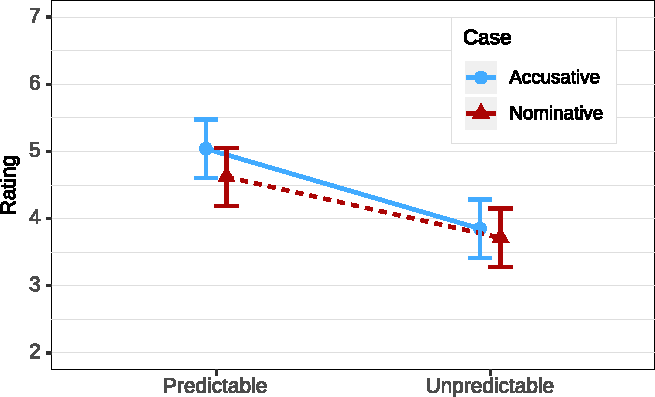
\includegraphics[scale=1]{figures/scripts_case_estimates}
\caption{Mean ratings and 95\% confidence intervals across conditions in experiment \ref{exp:scripts-rating-case}. \label{fig:scr-case-estimates}}
\end{figure}

\subsubsection{Results}
Figure \ref{fig:scr-case-estimates} shows the averaged ratings across conditions. The data were analyzed with CLMMs following the procedure described in Section \ref{sec:intro-stats}. The full model contained main effects for \textsc{Case}, \textsc{Predictability} and the \textsc{Position} of the item in the time-course of the experiment, as well as by-subject and by-item random intercepts and slopes for \textsc{Case}, \textsc{Predictability} and their interaction. Random effects of \textsc{Position} and its interaction with the other predictors were removed because models did not converge otherwise. The final model (see Table \ref{tab:scripts-case-estimates}) contained only a significant main effect for \textsc{Predictability} \clmmLR{10.04}{0.01}. Neither the main effect of \textsc{Case} \clmmLRnonsig{2.5}{0.1} nor its interaction with \textsc{Predictability} \clmmLRnonsig{1.78}{0.1} were significant.\largerpage

\begin{table}
\begin{tabular}{lccccc}
\lsptoprule
Predictor & Estimate & SE & $\chi^2$ &  $p$ &  \\   
\midrule
\textsc{Predictability} & -1.25 &  0.35 & 10.04 & \textless 0.01 & ** \\
\lspbottomrule
\end{tabular}
\caption{Fixed effects in the final CLMM for experiment \ref{exp:scripts-rating-case}. \label{tab:scripts-case-estimates}}
\end{table}

\subsubsection{Discussion}
The purpose of experiment \ref{exp:scripts-rating-case} was to test a mixed account\is{Mixed account} of fragments. Mixed accounts assume that speakers use two different mechanisms to interpret (and produce) fragments, which differ in their predictions with respect to case marking: If fragments are generated by ellipsis from full sentences, they can exhibit structural case marking\is{Case connectivity}, but if they are base-generated as genuine nonsententials\is{Nonsentential account}, they cannot. It is a natural assumption that speakers resort to ellipsis when there is a salient antecedent that allows resolution and to pragmatic inference when there is no such antecedent. Consequently, the mixed account\is{Mixed account} predicts that nominative\is{Nominative case} is rated\is{Acceptability rating task} as better than accusative\is{Accusative case} in the unpredictable condition, where it is more difficult to retrieve an antecedent for ellipsis. The absence of a significant interaction between \textsc{Case} and \textsc{Predictability} shows that this prediction is not borne out. Unpredictable fragments are significantly worse than predictable fragments, but this holds independently of case.

In contrast to experiment \ref{exp:case}, there was no significant main effect of \textsc{Case}. This might be due to a reduced accessibility of antecedents that require nominative\is{Nominative case} in the materials for experiment \ref{exp:scripts-rating-case} as compared to those used in experiment \ref{exp:case}. Whether this is correct could be tested with a further production study\is{Production task}. However, this goes beyond the scope of this experiment, which was designed to test whether nominative\is{Nominative case} is relatively more acceptable in unpredictable fragments.

Taken together, experiment \ref{exp:scripts-rating-case} provides further evidence against the nonsentential account\is{Nonsentential account}. Unlike what the nonsentential account\is{Nonsentential account} predicts, fragments are not rated\is{Acceptability rating task} better in nominative\is{Nominative case} than in accusative\is{Accusative case}. The pattern observed in experiment \ref{exp:scripts-rating-case} is unexpected both under the nonsentential\is{Nonsentential account} and the mixed account\is{Mixed account}.

\subsection{General discussion: Structural case marking}\largerpage
I presented three experiments that investigated whether fragments are derived from regular sentences by ellipsis or whether they are genuine nonsententials\is{Nonsentential account}. The experiments used structural case marking on discourse-initial\is{Fragment, discourse-initial} DP\is{Determiner phrase} fragments as a diagnostic for unarticulated structure. In minimalism\is{Minimalist program}, the framework that underlies both the nonsentential and most of the sentential accounts discussed in Chapter \ref{sec:chapter-theories}, structural case\is{Structural case} must be checked\is{Case feature} by a verbal head. If, as nonsententialists argue, there is no unarticulated structure in fragments, structural case marking must be unavailable in fragments. In contrast, according to sentential accounts there is an unarticulated verbal head in DP\is{Determiner phrase} fragments, so that they are expected to appear in structural case\is{Structural case} whenever they do in the corresponding full sentence\is{Case connectivity}. Experiments \ref{exp:case}--\ref{exp:scripts-rating-case} investigated this using the example of German\il{German}, where accusative\is{Accusative case} is a structural case and nominative\is{Nominative case} the default case\is{Default case}, if such a concept is to be assumed at all. Experiment \ref{exp:case} showed that if there is a salient antecedent that licenses accusative\is{Accusative case}, DP\is{Determiner phrase} fragments can appear in accusative\is{Accusative case} case. In fact, accusative\is{Accusative case} was rated\is{Acceptability rating task} even better than nominative\is{Nominative case}. This disconfirms the prediction of the nonsentential account\is{Nonsentential account} and in turn supports sentential accounts. Experiment \ref{exp:case-production} showed that in the context of my materials a full sentence requiring accusative\is{Accusative case} on the DP\is{Determiner phrase} was indeed more likely than one requiring nominative\is{Nominative case}. This finding further strengthens the interpretation of experiment \ref{exp:case} as evidence for connectivity effects\is{Case connectivity}. Finally, experiment \ref{exp:scripts-rating-case} explored the predictions of a mixed account\is{Mixed account} that assumes that fragment generation by ellipsis is possible, but restricted to contexts where an antecedent is available. Therefore, I tested whether nominative\is{Nominative case} is more acceptable when the corresponding sentence is relatively unpredictable. Since there was no such effect, the data speak against the mixed account\is{Mixed account} that I sketched.

It must be emphasized that this interpretation of the data presupposes that the categorical difference between structural and inherent\is{Inherent case} case assumed by \citet{barton.progovac2005} is correct. This distinction is crucial to the nonsentential account\is{Nonsentential account}, since \citet{barton.progovac2005} rely on it to explain crosslinguistic differences between English\il{English} and Serbian\il{Bosnian/Croatian/Serbian} as well as acceptability contrasts within English\il{English}. Nonsentential accounts that do not rely on the inherent\is{Inherent case}/structural case distinction as heavily as \citet{barton.progovac2005} do, like analyses in the simpler syntax framework\is{Simpler syntax} \citep{culicover.jackendoff2005} or in HPSG\is{HPSG} \citep{ginzburg.sag2000, fernandez.ginzburg2002} might still be able to explain the data. The data are also in line with the idea that fragments are ungrammatical, but can point toward the meaning intended by a speaker, as suggested by \citet{bergen.goodman2015}\is{Ungrammaticality of fragments}. Since accusative\is{Accusative case} case in fragments might indicate that the DP\is{Determiner phrase} fragment is to be interpreted as patient or object, a preference for accusative\is{Accusative case} is expected under this account, if the DP\is{Determiner phrase} fragment is the object of a transitive verb in a corresponding complete sentence. 

Furthermore, the predictions of the nonsentential account\is{Nonsentential account} also rely on the classification of a particular case as structural or inherent\is{Inherent case}. \citet{barton.progovac2005} argue that nominative\is{Nominative case} is structural case in English\il{English}, but default case\is{Default case} in Serbian\il{Bosnian/Croatian/Serbian}, so that nominative\is{Nominative case} DP\is{Determiner phrase} fragments are predicted to be ungrammatical in English\il{English}, but not in Serbian\il{Bosnian/Croatian/Serbian}. The conclusions that I draw from my data rely on the assumption that accusative\is{Accusative case} is indeed structural case in German\il{German}. \citet{progovac.etal2006} argued that accusative\is{Accusative case} is inherent\is{Inherent case}, semantically interpretable, case in German\il{German}, and if this is correct, the nonsentential account\is{Nonsentential account} would correctly predict German\il{German} accusative\is{Accusative case} DP\is{Determiner phrase} fragments to be acceptable. I argued above that, given the tests used by \citet{progovac.etal2006} for Serbian\il{Bosnian/Croatian/Serbian}, accusative\is{Accusative case} must be classified as structural case in German\il{German}, so that the nonsentential account\is{Nonsentential account} makes incorrect predictions.\largerpage[-1]

Even though the experiments did not explicitly test the predictions of a con\-struc\-tion-\is{Construction grammar}based account, they suggest that the acceptability of accusative\is{Accusative case} case cannot be explained by the assumption of a conventionalized construction like e.g. $\langle$DP\is{Determiner phrase}$\rangle$\textsubscript{Acc}: Both in experiments \ref{exp:case} and \ref{exp:scripts-rating-case}, the acceptability of accusative\is{Accusative case} does not vary as a function of the predictability or degree of conventionalization of the fragment. Of course this does not rule out the possibility that some fragments are stored as constructions in the mental lexicon, but this cannot explain the acceptability of accusative\is{Accusative case} DP\is{Determiner phrase} fragments in my experiments.

Taken together, the experiments presented in this section support a sentential analysis of fragments against the nonsentential account\is{Nonsentential account} by \citet{barton.progovac2005}. They furthermore empirically confirm two properties of fragments that have to be taken into account in the investigation of fragment usage: Fragments exhibit case connectivity\is{Case connectivity} and that they can appear in structural case\is{Structural case}.

Having established that fragments are underlyingly sentential, this leads to my second main research question on the syntax of fragments, that is, whether the generation of fragments involves movement to the left periphery \citep{merchant2004}\is{Movement and deletion account} or whether fragments result from in situ deletion \citep{reich2007}\is{In situ deletion account}.

\section{Movement restrictions: Preposition omission}\label{sec:pstranding}
\largerpage[-1]

The experiments in Section \ref{sec:experiments-case} provided evidence for unarticulated syntactic structure in fragments, in particular for a silent verbal head that checks accusative\is{Accusative case} structural case\is{Structural case} in DP fragments. In the remainder of this chapter I investigate which kind of structure underlies fragments. The main controversy with respect to this question is whether the derivation of fragments involves obligatory movement to the left periphery. In Sections \ref{sec:theories-sentential} and \ref{sec:theories-predictions-movement} I outlined the positions: On the one hand, there is \citepos{merchant2004} influential movement and deletion\is{Movement and deletion account} account, which has been more recently adopted and partially modified by other researchers \citep[see e.g.][]{aelbrecht2009, sato2011,weir2014, doring2016, saab.liptak2016,  murphy2018} and assumes that the derivation of fragments involves obligatory movement to the left periphery. On the other hand, in situ deletion\is{In situ deletion account} accounts \citep{reich2007, ott.struckmeier2016, griffiths.etal2018} derive fragments from regular sentences without assuming this obligatory movement step.

Since the in situ deletion\is{In situ deletion account} approach does not require an additional movement operation in fragments, it is derivationally simpler. Therefore, the movement and deletion account\is{Movement and deletion account} requires additional evidence for movement in fragments. Such evidence consists in effects of movement restrictions\is{Movement restriction} on the form of fragments, which are then taken to indicate that left dislocation is a necessary step in the generation of fragments. \citet{merchant2004} discusses a series of such similarities between fragments and dislocation constructions, but even the brief discussion in Section \ref{sec:theories-predictions-movement} showed that not all of these parallelisms constitute genuine evidence for movement, because some of them can be explained under a non-movement account as well. Since the in situ deletion\is{In situ deletion account} account is derivationally less complex than movement and deletion\is{Movement and deletion account}, I assume that it is the null hypothesis.%
%
\footnote{Actually the nonsentential account\is{Nonsentential account} is even simpler, but I rejected it in the preceding section because it does not capture the empirical picture correctly.}\afterfn%
%
Consequently, the movement and deletion\is{Movement and deletion account} account is only superior to in situ deletion\is{In situ deletion account} if there are parallelisms between fragments and left dislocation that cannot be explained by the in situ deletion\is{In situ deletion account} account. In my experiments I focus on three movement restrictions\is{Movement restriction} that have been claimed to or that might constrain the form of fragments. This section investigates restrictions on preposition stranding\is{Preposition stranding} and omission\is{Preposition omission} in German\il{German}, in Section \ref{sec:ccs} I address complement clause\is{Complement clause} topicalization and in Section \ref{sec:mvb} multiple prefield\is{Prefield} constituents in German\il{German}.

\subsection{Preposition omission as evidence for movement}\label{sec:pstranding-background}
\largerpage[-1]

\is{P-Stranding Generalization|(}
\subsubsection{The P-Stranding Generalization}\label{sec:pstranding-background-psg}
Among the movement restrictions\is{Movement restriction} that \citet{merchant2004} presents as evidence for his theory, the most compelling one is his \textit{P-Stranding Generalization}\is{P-Stranding Generalization} (PSG, in what follows). In a nutshell, the PSG\is{P-Stranding Generalization} states that only in those languages that allow for P-stranding\is{Preposition stranding} under regular \textit{wh}-movement it is possible to omit prepositions\is{Preposition omission} under sluicing\is{Sluicing} and in fragments. \citeauthor{merchant2004} takes this as evidence that P-stranding is a necessary step in the derivation of preposition-less answers\is{Fragment, short answer} to questions where the \textit{wh}-phrase corresponding to the answer is embedded within a PP\is{Preposition phrase}. English\il{English} is a typical example of a P-stranding language \Next. 

\ex. Who was Peter talking with?\hfill\citep[685]{merchant2004}\\
Mary.

Originally, \citet{merchant2001} introduced the PSG\is{P-Stranding Generalization} as evidence for his movement and deletion\is{Movement and deletion account} account of sluicing\is{Sluicing}. He presents introspective data from a relatively large and typologically diverse sample of languages%
%
\footnote{The data are from Arabic\il{Arabic}, Basque\il{Basque}, Czech\il{Czech}, Danish\il{Danish}, English\il{English}, Frisian\il{Frisian}, German\il{German}, Greek\il{Greek}, Hebrew\il{Hebrew}, Icelandic\il{Icelandic}, Irish\il{Irish}, Norwegian\il{Norwegian}, Polish\il{Polish}, Russian\il{Russian},  Serbo\il{Bosnian/Croatian/Serbian}-Croatian, Slovene\il{Slovene}, Swedish\il{Swedish} and Yiddish\il{Yiddish}.}\afterfn%
%
that overall show the predicted pattern. The contrast between languages that allow for P-stranding\is{Preposition stranding} and those with obligatorily pied-piping\is{Pied-piping} is exemplified in \Next and \NNext for English\il{English} and German\il{German}, respectively: English\il{English} allows for P-stranding\is{Preposition stranding} in \textit{wh}-questions \Next[a] and preposition omission\is{Preposition omission} under sluicing\is{Sluicing} \Next[b], whereas in German\il{German} the preposition is always pied-piped\is{Pied-piping} in \textit{wh}-questions \NNext[a] and realized in sluices\is{Sluicing} \NNext[b].

\ex.
\a. Who was he talking with? \label{pst-english-question}\hfill \citep[666]{merchant2004}
\b. Peter was talking with someone, but I don’t know (with) who.

\ex. 
\ag. *Wem hat sie mit gesprochen?\label{ex:pst-german-q}\\
Who.\textsc{dat} has she with talked\\
\trans{With whom was she talking?}\exsourceraised{\citep[667]{merchant2004}}
\bg. Anna hat mit jemandem gesprochen, aber ich wei\ss {} nicht, *(mit) wem. \hfill\\
Anna has with somebody.\textsc{dat} spoken but I know not \mbox{~~}with who.\textsc{dat}\\
\trans{Anna was talking with somebody, but I don't know (with) who.}

The reasoning behind the PSG\is{P-Stranding Generalization} is that, if sluicing\is{Sluicing} is generated by regular \textit{wh}-movement as discussed above, the preposition cannot be omitted\is{Preposition omission} in German\il{German}, because this would require P-stranding\is{Preposition stranding} to occur during the derivation \Next. As P-stranding\is{Preposition stranding} is available in English\il{English} \LLast[a], but not in German\il{German} \Last[a], the corresponding sluice \LLast[b]/\Last[b] is grammatical in English\il{English}, but not in German\il{German}.%
%
\footnote{In German\il{German}, there are a few constructions which are similar to P-stranding\is{Preposition stranding}. In \Next, the particle \textit{her} contained in the complex \textit{wh}-phrase \textit{woher} can be stranded\is{Preposition stranding}, but in contrast to the PPs\is{Preposition phrase} providing evidence for the PSG\is{P-Stranding Generalization}, the moved element appears to the left of \textit{her} if no extraction occurs. See e.g. \citet{vanriemsdijk1978} for an analysis of such extractions in Dutch\il{Dutch}.

\ex. \ag. Wo hast du das Buch denn her?\\
	  where have you the book \textsc{prt} \textit{her}\\ 
\bg. Woher hast du das Buch denn?\\
	  where.from have you the book \textsc{prt} \textit{her}\\ 
	  \trans{Where did you get the book from?}

}\afterfn%
%

\ex. Peter was talking with someone, but I don't know who\textsubscript{i} \sout{Peter was talking with \textit{t}\textsubscript{i}}.

In his \citeyear{merchant2004} article, \citeauthor{merchant2004} extends this analysis to fragments\is{Fragment, short answer}. He argues that only languages that have P-stranding\is{Preposition stranding} allow for the omission of the preposition\is{Preposition omission} in short answers to questions whose \textit{wh}-phrase is the complement of a preposition. Again, the observation is supported by crosslinguistic data.%
% 
\footnote{The data are from Bulgarian\il{Bulgarian}, Czech\il{Czech}, Danish\il{Danish}, English\il{English}, German\il{German}, Greek\il{Greek}, Hebrew\il{Hebrew}, Icelandic\il{Icelandic}, Norwegian\il{Norwegian}, Russian\il{Russian}, Swedish\il{Swedish} and Yiddish\il{Yiddish} \citep[685--687]{merchant2004}.}\afterfn%
%
The contrast is exemplified here for English\il{English} \Next and German\il{German} \NNext.

\ex. 
Who was Peter talking with? \hfill\citep[685]{merchant2004} \label{ex:pstranding-fragments-english}\\
(With) Mary.

\exg. Mit wem hat Anna gesprochen?\\
with whom has Anna spoken?\\
\trans{Who was Anna talking to?} \exsourceraised{\citep[686]{merchant2004} \label{ex:pstranding-fragments-german}}
\ag. Mit dem Hans.\\
with the.\textsc{dat} Hans\\
\trans{With Hans.}
\bg. *Dem Hans.\\
the.\textsc{dat} Hans\\
\trans{Hans.}

\citeauthor{merchant2004}'s account of this pattern is parallel to his analysis of sluicing\is{Sluicing}. He assigns the underlying structures in \Next to the fragments in \LLast and \Last[b]. Since  he derives fragments by movement to the left periphery, the derivation of the DP\is{Determiner phrase} short answer\is{Fragment, short answer} requires P-stranding\is{Preposition stranding}, which is available in English\il{English} \Next[a], but not in German\il{German} \Next[b]. Note that fronting a non-contrastive object \Next[a] is marked in English\il{English}, so that a movement-based account\is{Movement and deletion account} probably has to assume exceptional movement\is{Exceptional movement account} \citep{weir2014}: The acceptability of the fragment does not pattern with the degradedness of the corresponding left dislocation.\largerpage

\ex. \a. Mary\textsubscript{i} Peter talked to \textit{t}\textsubscript{i}.
    \b. *[Dem Hans]\textsubscript{i} hat Anna mit \textit{t}\textsubscript{i} gesprochen. 

Before going into further detail, it must be noted that the crosslinguistic correlation between the availability of P-stranding\is{Preposition stranding} and the acceptability of preposition omission\is{Preposition omission} under ellipsis is not perfect: There are languages which seem to allow for preposition omissions\is{Preposition omission} even though they lack P-stranding\is{Preposition stranding} and vice versa. However, for these data to constitute evidence against the PSG\is{P-Stranding Generalization}, it is necessary to rule out alternative sources for these fragments and sluices\is{Sluicing}, which do not require P-stranding\is{Preposition stranding}. For instance, \citet[176]{rodrigues.etal2009} show that in Spanish\il{Spanish} preposition omission\is{Preposition omission} under sluicing\is{Sluicing} can be acceptable \Next[a] even though P-stranding\is{Preposition stranding} in questions is not \Next[b].

\ex.
\ag. Juan ha hablado con una chica pero no sé cuál.\\
Juan has talked with a girl but not know which\\
\trans{Juan has talked with a girl but I don't know which one}
\bg. *¿Qué chica ha hablado Juan con?\\
what girl has talked Juan with\\
\trans{Which girl did John talk to?}

Since \Last[b] suggests that extraction out of PPs\is{Preposition phrase} is ungrammatical, the movement account cannot derive the grammatical sluice\is{Sluicing} \textit{cuál} `which one' by extraction out of a PP \textit{con cuál}. \citet[178]{rodrigues.etal2009} argue that \Last[a] can be derived from a cleft\is{Cleft} structure like \Next, which does not require the ungrammatical extraction out of a PP\is{Preposition phrase}. Similar accounts have been proposed by \citet{szczegielniak2008} for Polish\il{Polish}, \citet{vancraenenbroeck2010} for English\il{English} and \citet{sato2011} for Indonesian. More recently, it has been controversially debated whether \textit{all} of the data conflicting with the PSG\is{P-Stranding Generalization} can be explained by the cleft\is{Cleft} hypothesis.%
%
\footnote{See e.g. \citet{stigliano2018, stigliano2019} for Spanish\il{Spanish} and \citet{nykiel2013} for Polish\il{Polish}.}\afterfn%
%

\exg. Juan ha hablado con una chica pero no sé cuál es la chica con la que ha hablado Juan.\\
Juan has talked with a girl but not know which is the girl with the that has talked Juan\\
\trans{Juan has talked with a girl but I don't know which one was the girl with whom Juan talked.}

For German\il{German}, \citet{lemkeaccepted} shows that preposition omission in German are rated as more acceptable when the DP\is{Determiner phrase} is a proper noun, which is not headed by an overt article\is{Article omission} \Next than when the DP\is{Determiner phrase} has an article, like \ref{ex:pstranding-fragments-german}.\largerpage[2]

\exg. 
?(Mit) Hans.\label{ex:eigenname}\\
with Hans\\
\trans{(With) Hans.}

Given the discussion in the literature it is at least questionable whether the derivation from clefts\is{Cleft} is a crosslinguistically plausible explanation for the empirically observed apparent exceptions to the PSG\is{P-Stranding Generalization}. Furthermore, a movement-based theory of fragments\is{Movement and deletion account} that assumes that their derivation is possible both from regular leftward movement and clefts\is{Cleft} must explain why and when speakers pursue each of these strategies and hence produce the corresponding fragment. Providing an answer to these questions is beyond the scope of this book, since they presuppose a movement-based account\is{Movement and deletion account}, which I do not adopt a priori. However, the possibility that preposition-less fragments or sluices\is{Sluicing} have been derived from clefts\is{Cleft} must be obviously taken into account. Following the line of reasoning that I pursue in order to investigate unarticulated structure, fragments that are derived by ellipsis from clefts\is{Cleft} must exhibit the morphosyntactic properties of the corresponding phrase in that cleft\is{Cleft}. In the case of preposition omission\is{Preposition omission}, this concerns morphological case marking on the DP\is{Determiner phrase} fragments that result from preposition omission\is{Preposition omission}. For instance, in German\il{German}, DP\is{Determiner phrase}s that are the complement of a preposition exhibit prepositional case\is{Prepositional case} marking (accusative\is{Accusative case}, dative\is{Dative case} or genitive\is{Genitive case}) \Next[a], whereas in a cleft\is{Cleft} the DP\is{Determiner phrase} appears obligatorily in nominative\is{Nominative case} case \Next[b]. The cleft\is{Cleft} account could thus potentially explain why proper nouns, which are not marked for case and can hence be interpreted as nominative\is{Nominative case} are acceptable in \ref{ex:eigenname}.%
%
\footnote{This prediction is specific to German\il{German} and does not necessarily hold for all languages with morphological case marking. For instance, \citet{szczegielniak2008} derives Polish\il{Polish} preposition-less DP\is{Determiner phrase} fragments from a cleft\is{Cleft} construction where the DP\is{Determiner phrase} appears in prepositional case\is{Prepositional case}. German\il{German} however has no such construction.}\afterfn%
%
Consequently, if a DP\is{Determiner phrase} fragment cannot be derived from \Next[a] due to the unavailability of P-stranding\is{Preposition stranding} in German\il{German}, but from the cleft\is{Cleft} in \Next[b], it must always appear in nominative\is{Nominative case} case.%
%
\footnote{A similar empirical prediction is implied by the dicussion on \textit{that is}-ellipsis\is{That is-ellipsis} in \citet{merchant2004}, who argues that the copula and a pronoun like \textit{it} are inherently given and can be omitted in the absence of a corresponding \textit{linguistic} antecedent. Therefore in \ref{ex:package-cleft} a DP\is{Determiner phrase} fragment answer\is{Fragment, short answer} could be also derived from the sentence \Next. Like the cleft\is{Cleft} account, this analysis also predicts nominative\is{Nominative case} case on the DP\is{Determiner phrase} fragment.

\exg. Mein Vater war es.\\
      my.\textsc{nom} father was it\\
      \trans{My father it was.}
      
However, at least for sluicing\is{Sluicing} it seems doubtful that such a \textit{that is} construction is the structure underlying preposition omission\is{Preposition omission} data in German\il{German}. \citet{lemke.etalaccepted} show that in a production task\is{Production task} subjects frequently produce constructions like \Next[a], but not their sluiced counterparts in \Next[b]. In contrast, when the potentially reduced phrase was introduced by a PP\is{Preposition phrase} that matches the category of the antecedent \textit{mit jemandem}, like in \NNext, sluicing was relatively frequent. In an acceptability rating\is{Acceptability rating task} study \citet{lemke.etalaccepted} find that \Next[b] is heavily degraded as compared to the sluice derived from \NNext. This provides further evidence that such instances of preposition omission\is{Preposition omission} examples in German\il{German} are not derived from \textit{that is} constructions.

\ex. \ag. Hans hat mit jemandem getanzt, aber ich weiß nicht, wer das war.\\
          Hans has with somebody danced, but I know not who that was\\
          \trans{Hans danced with somebody, but I don't know who that was.}
      \bg. *Hans hat mit jemandem getanzt, aber ich weiß nicht, wer.\\
          Hans has with somebody danced, but I know not who\\
          \trans{Hans danced with somebody, but I don't know who.}     
          
\ex. Hans hat mit jemandem getanzt, aber ich weiß nicht, mit wem (Hans getanzt hat).\\
          Hans has with somebody danced, but I know not with who \phantom{(}Hans danced has\\
          \trans{Hans danced with somebody, but I don't know with whom Hans danced.}             
         
   }\afterfn%
%

\exg. Für wen ist das Päckchen?\label{ex:package-cleft}\\ 
      for who\textsc{acc} is the package\\
      \trans{For whom is the package?}
      \ag. Es ist für meinen Vater.\\
      it is for my.\textsc{acc} father\\
      \trans{It is for my father.}\exsourceraised{PP fronting}
      \bg. Es ist mein Vater, für den das Päckchen ist.\\ 
      it is my.\textsc{nom} father for who.\textsc{acc} the package is\\
      \trans{It is my father for whom is the present.}\exsourceraised{Cleft}
      
I return to this issue in experiment \ref{exp:pstranding-defaultcase}, which compares the acceptability\is{Acceptability rating task} of PP\is{Preposition phrase} short answers to that of nominative\is{Nominative case} and prepositional case\is{Prepositional case}-marked DP\is{Determiner phrase} short answers\is{Fragment, short answer}. Before turning to the empirical investigation of the predictions made by the PSG\is{P-Stranding Generalization}, I briefly discuss how the PSG\is{P-Stranding Generalization} can be theoretically motivated in a generative\is{Generative grammar} framework rather than just postulating it as a descriptively appropriate generalization. This is particularly important because some implementations of the PSG\is{P-Stranding Generalization} explain the relevant data without assuming movement at all, and this would weaken the status of the PSG as evidence for movement in fragments\is{Movement and deletion account}.

\is{Minimalist program|(}
\is{Pied-piping|(}

\subsubsection{P-stranding and pied-piping in minimalism}
\label{sec:pstranding-background-mp}
\citet{merchant2004} leaves open the question of why P-stranding\is{Preposition stranding} is possible in English\il{English}, but not in German\il{German}. In \citet{merchant2001}, he makes a tentative suggestion in terms of an analysis of prepositions as case markers, but the idea is not spelled out in detail. However, as I argued above, the processes underlying a movement restriction\is{Movement restriction} that is taken to support movement and deletion\is{Movement and deletion account} are not trivial, because they might also facilitate non-movement explanations for the data (which might also explain as well, but for independent reasons, why movement is blocked). In what follows, I briefly illustrate how the viability of specific accounts of fragments relies on the analysis that P-stranding\is{Preposition stranding}/pied-piping\is{Pied-piping} itself receives.

Pied-piping\is{Pied-piping} is specifically problematic in minimalism\is{Minimalist program}, because in this framework movement is in general assumed to be a feature-driven last resort operation. This implies that (i) movement is never optional (because it is the last resort to save derivations from crashing) and (ii) that the constituent that is moved hosts the feature that needs to be checked. However, in pied-piping\is{Pied-piping} not only this constituent itself, but a superordinate constituent is moved, which \textit{contains} the constituent hosting the feature. This is exemplified in Figure \ref{ex:pst-mp-pp} for \textit{wh}-movement in a question like \Next: Not only the \textit{wh}-phrase hosting the uninterpretable \textit{wh}-feature, but the complete PP\is{Preposition phrase} appears in [Spec, PP\is{Preposition phrase}]. Unless exceptional movement\is{Exceptional movement account} \citep{weir2014} is assumed, which is not feature-driven, this concerns the generation of fragments under the movement and deletion\is{Movement and deletion account} account, which needs to assume some kind of (probably focus-related) feature in order to motivate movement to [Spec, FP].

\ex. For whom is the present? \label{ex:pst-mp}

\begin{figure}
 \Tree [.CP [.PP\textsubscript{i} [.P for ] [.DP\textsuperscript{\textit{u}wh} whom\textsuperscript{\textit{u}wh} ] ] [.C' C\textsuperscript{wh} [.TP \edge[roof]; {is the present \textit{t}\textsubscript{i}} ] ] ]
 
  \caption{Derivation of \ref{ex:pst-mp} under a pied-piping analysis. In this analysis, only the DP hosts the \textit{wh}-feature.\label{ex:pst-mp-pp}}
\end{figure}


\begin{sloppypar}
\noindent 
One possible solution to this problem is the assumption of \textit{feature percolation}\is{Feature percolation} \citep{chomsky1973, grimshaw2000}. The idea is that under certain conditions syntactic features can  `percolate' to projections outside the maximal projection whose head hosts the feature. In \Last, for instance, the \textit{wh}-feature would percolate to the PP\is{Preposition phrase} level, so that the complete PP\is{Preposition phrase} is marked [\textit{u}wh] and must move to [Spec, CP\is{Complementizer phrase}]. As Figure \ref{ex:pst-mp-fp} shows, technically speaking, under this analysis there is no pied-piping\is{Pied-piping} in the proper sense, because the PP\is{Preposition phrase} as a whole just behaves like any other \textit{wh}-phrase. This idea has been explicitly applied to prepositional pied-piping\is{Pied-piping} in \textit{wh}-questions \citep{trissler.lutz1992, grimshaw2000,  trissler2000, yoon2001,  lasnik2006, sato2011}. As there is no reason to assume that a concept such as feature percolation\is{Feature percolation} is restricted to \textit{wh}-questions, it can be immediately applied to the movement operations that derive fragments according to \citeauthor{merchant2004}'s theory\is{Movement and deletion account}. If movement in frag\-ments is driven by some focus-related feature and the choice between P-stranding\is{Preposition stranding} and pied-piping\is{Pied-piping} depends on whether this feature percolates\is{Feature percolation} to PP\is{Preposition phrase}, the structures underlying P-stranding\is{Preposition stranding} and pied-piping\is{Pied-piping} would only differ in whether the complete PP\is{Preposition phrase}, or only the DP\is{Determiner phrase} has the focus feature \Next.
\end{sloppypar}

\begin{figure}

\Tree [.CP {[For whom]}\textsuperscript{\textit{u}wh}\textsubscript{i} [.C' C\textsuperscript{wh} [.TP \edge[roof]; {is the present \textit{t}\textsubscript{i}} ] ] ]

 \caption{Derivation of \ref{ex:pst-mp} under a feature percolation analysis. In this analysis, the complete PP is marked as [+\textit{wh}] as the result of feature percolation.\label{ex:pst-mp-fp}}
\end{figure}
%

\ex. \label{ex:pst-focus-english}
\a. \sout{This package is} [for my father]\textsubscript{\textsc{F}}.
\b. \sout{This package is for} [my father]\textsubscript{\textsc{F}}.

Now, if the preposition is obligatorily pied-piped\is{Pied-piping} for whatever reason (see the references below and footnote \ref{fn:pstranding-alternatives} for some hypotheses), this indicates that the focus structure licensing P-stranding\is{Preposition stranding}, i.e. focusing the DP\is{Determiner phrase} only, is not available in German\il{German} \Next. This pattern however is exactly what the in situ deletion\is{In situ deletion account} account requires in order to explain the contrast between English\il{English} and German\il{German}. Since it assumes that only the non-focused parts of the utterance may be deleted, the ellipsis of the preposition is never licensed in German\il{German}, because the corresponding focus structure \Next[b] is unavailable in this language. Taken together, if it is assumed that in such examples the PP\is{Preposition phrase} is marked with the feature triggering movement, the movement and deletion\is{Movement and deletion account} account makes exactly the same prediction as in situ deletion\is{In situ deletion account} and therefore does not gain larger explanatory power. This holds for any version of the theory that assumes feature percolation\is{Feature percolation}.

\ex. \label{ex:pst-focus-german}
\a. \sout{Das Päckchen ist} [für meinen Vater]\textsubscript{F}. 
\b. *\sout{Das Päckchen ist für} [meinen Vater]\textsubscript{F}.

If the preposition omission\is{Preposition omission} data are taken to be evidence for movement, there must be a genuine movement restriction\is{Movement restriction}, which has no effect on the potential form of fragments if the PP\is{Preposition phrase} remains in situ. Such a movement restriction\is{Movement restriction} could be the assumption that PP\is{Preposition phrase} is an island\is{Island} for extraction in German\il{German}, but not in English\il{English}, as has been first suggested by \citet{vanriemsdijk1978}. In simplified terms, he argues that the preposition can be reanalyzed in English\il{English} as forming a syntactic unit with the verb, so that it can be separated from the noun by movement.%
%
\footnote{This also predicts an asymmetry between prepositional objects and adjuncts\is{Adjunct}, because the preposition is subcategorized only in the case of the former. \citet{pullum.huddleston2002} observe that indeed extraction out of adjunct PPs\is{Preposition phrase} seems to be dispreferred as compared to prepositional objects. This is also empirically supported by my experiment \ref{exp:pstranding-production}, where the overall preference for omitting prepositions\is{Preposition omission} in short answers\is{Fragment, short answer} was reduced for adjunct\is{Adjunct} PPs\is{Preposition phrase} as compared to argument PPs\is{Preposition phrase}.}\afterfn%
%
More recently, \citet{abels2003} has picked up the idea of structural differences between the PP\is{Preposition phrase} in languages that have and those that lack P-stranding\is{Preposition stranding}. \citeauthor{abels2003} argues that PP\is{Preposition phrase} is a phase in German\il{German}, but not in English\il{English}. A phase can only be evacuated through its left edge, i.e. the specifier of the highest projection within this phase. From this perspective, extraction of the complement of P out of the PP\is{Preposition phrase} is possible in English\il{English}, but not in German\il{German}, because it would have to be first moved to [Spec, PP\is{Preposition phrase}] in German\il{German}. 

Movement of the complement of a phrase head to its specifier is not possible, because movement occurs only for feature checking purposes and features can be checked in a head-complement relation.%
%
\footnote{In a later version of his theory, \citet{abels2012} argues that PP\is{Preposition phrase} is always a phase. In this theory, the preposition is the head of the phase, which can be evacuated only through its edge, [Spec, PP\is{Preposition phrase}]. The complement of P can never be moved to this position, because movement must be triggered by feature checking requirements in minimalism\is{Minimalist program}. The complement is already in a local configuration with the P head that allows for feature checking, so that no movement is required and consequently licensed. \citet[245--268]{abels2012} argues that the critical difference between languages that allow P-stranding\is{Preposition stranding} and those that do not is that the former involve additional structure (a projection headed by an empty morpheme) between the preposition and the DP\is{Determiner phrase}. Consequently, this morpheme, but not the DP\is{Determiner phrase} is the complement of P. Under this analysis, P-stranding\is{Preposition stranding} involves movement out of a more deeply embedded position within the PP\is{Preposition phrase}, which is also available in languages without P-stranding\is{Preposition stranding}, like German\il{German} \Next. \citeauthor{abels2012} motivates the assumption of the empty morpheme in languages that do not have P-stranding\is{Preposition stranding} with the argument that it has overt counterparts in some languages.

\exg. Was (für Bücher) hast du (für Bücher) gelesen (für Bücher)?\\
      what for books have you for books read for books\\
     \trans{What (kind of books) have you read?}\exsourceraised{\citep[255]{abels2012}}

}\afterfn%
%

Such structural differences between the German\il{German} and English\il{English} PP\is{Preposition phrase} might explain why extraction out of the PP\is{Preposition phrase} is blocked in German\il{German}, but it does not explain why the PP\is{Preposition phrase} can be moved as a whole. Under the assumption of feature-driven movement, if feature percolation\is{Feature percolation} is ruled out, this approach requires an additional explanation for why the PP\is{Preposition phrase} can be moved as a whole in case extraction is not possible. This could be modeled by integrating optimality-theoretic violable constraints on locality in the minimalist\is{Minimalist program} framework, as \citet{heck2008} suggests, but such additional assumptions clearly complicate the overall theoretical framework. The phase-based account is also compatible with \citepos{weir2014} assumption of exceptional movement\is{Exceptional movement account}. \citeauthor{weir2014}'s account in principle requires fronting the focused phrase in order to evacuate it from the ellipsis site, but according to the theory, it can carry along ``any material which it might need to pied-pipe'' \citep[186]{weir2014}. If the complement of the preposition cannot be extracted for independent reasons in languages which, like German\il{German}, do not have P-stranding\is{Preposition stranding}, pied-piping\is{Pied-piping} saves the derivation from crashing. Recall that this movement occurs only for PF reasons, specifically, the incompatibility of the pitch accent marking focus with ellipsis. The fact that the fragment is focused does not imply the existence a focus feature that needs to be checked, hence \citeauthor{weir2014} does not need to assume feature percolation\is{Feature percolation}.\largerpage[-1]

The brief discussion in this section showed that the theoretical analysis of P-stranding\is{Preposition stranding} and pied-piping\is{Pied-piping}%
%
\footnote{\label{fn:pstranding-alternatives}
Besides the accounts referred to so far, among the syntactic accounts, \citet{sato2011} assumes that in German\il{German} PPs\is{Preposition phrase}, but not in English\il{English} ones, the determiner\is{Determiner phrase} in D is head-moved to P. Other researchers,  as \citet{tokizaki2010} and \citet{philippova2014}, claim that P-stranding\is{Preposition stranding} is never syntactically blocked, but ruled out when it yields prosodically ill-formed structures.}\afterfn%
%
determines whether the correlation between preposition omission\is{Preposition omission} and P-stranding\is{Preposition stranding} in fragments evidences a movement restriction\is{Movement restriction} or whether it is expected under non-movement accounts as well. Advocates of movement and deletion\is{Movement and deletion account} would have to commit to one of these analyses but as for now there is no consensus about which of the analyses discussed so far is correct. The picture becomes even more complicated when the difference between acceptable and unacceptable instances of P-stranding\is{Preposition stranding} \textit{within} a P-stranding\is{Preposition stranding} language (see footnote \ref{fn:piedpiping-en-restrictions} below for English\il{English}) is taken into account. Finally, if the availability of P-stranding\is{Preposition stranding} and preposition omission\is{Preposition omission} in fragments is attributed to a structural difference between English\il{English} and German\il{German} PPs\is{Preposition phrase}, the apparent optionality of P-stranding\is{Preposition stranding} in contexts that allow for it in English\il{English} also calls for an explanation, because in minimalism\is{Minimalist program} syntactic operations are not optional. Consequently, before interpreting the P-stranding\is{Preposition stranding} generalization as evidence for movement, there should be a more explicit account of pied-piping\is{Pied-piping} and P-stranding\is{Preposition stranding}.

Solving this intricate theoretical problem is beyond the scope of this work. The discussion in this section showed that if pied-piping\is{Pied-piping} is explained through feature percolation\is{Feature percolation} or when the structured propositions approach by \citet{reich2002} (see Section \ref{sec:psg-alternatives-structured}) is pursued, movement and deletion\is{Movement and deletion account} and in situ deletion\is{In situ deletion account} make the same empirical predictions. However, it also showed that if feature percolation\is{Feature percolation} is rejected and the PSG\is{P-Stranding Generalization} is explained with a ban on extraction out of PPs\is{Preposition phrase} in German\il{German}, as suggested by \citet{abels2003, abels2012}, the PSG\is{P-Stranding Generalization} provides evidence for the movement and deletion\is{Movement and deletion account} account. Therefore, in what follows I investigate first whether the general pattern that the PSG\is{P-Stranding Generalization} predicts for fragments holds in German\il{German} and English\il{English} (experiments \ref{exp:pstranding-german} and \ref{exp:pstranding-english}), before I explore potential non-movement explanations for the data. If the pattern found in experiments \ref{exp:pstranding-german} and \ref{exp:pstranding-english} can be explained without the assumption of movement, the assumption of the additional movement step is empirically unmotivated. Experiment \ref{exp:pstranding-defaultcase} tests a hypothesis that has been first mentioned in \citet{barton.progovac2005}, who attribute the impossibility of omitting the preposition\is{Preposition omission} in German\il{German} to its involvement in prepositional case\is{Prepositional case} checking. This prediction is not borne out. Experiment \ref{exp:pstranding-production} provides evidence for a nonsyntactic parallelism between question and answer, which can be accounted for in terms of processing\is{Processing effort} \citep{levelt.kelter1982, nykiel2017} or a structured proposition analysis of question semantics \citep{reich2002, reich2007}.
\is{P-Stranding Generalization|)}
\is{Pied-piping|)}
\is{Minimalist program|)}


\refstepcounter{expcounter}\label{exp:pstranding-german}
\subsection{Experiment \ref{exp:pstranding-german}: Preposition omission in German} 
\label{sec:pstranding-german}

\subsubsection{Background} \label{sec:pstranding-german-background}
Experiments \ref{exp:pstranding-german} and \ref{exp:pstranding-english} empirically test the predictions of the PSG\is{P-Stranding Generalization} for German\il{German} and English\il{English} respectively. If the PSG\is{P-Stranding Generalization} indeed is the result of a movement restriction\is{Movement restriction}, the movement and deletion\is{Movement and deletion account} account predicts that preposition omission\is{Preposition omission} in fragments is possible in English\il{English} but not in German\il{German}. Furthermore, experiment \ref{exp:pstranding-german} establishes a baseline for the follow-up experiment \ref{exp:pstranding-defaultcase}.

For German\il{German}, \citet{merchant.etal2013} conducted a similar experiment\is{Acceptability rating task} that confirms the introspective judgments for  question-answer pairs like \ref{ex:pstranding-fragments-german}, which I repeat here as \Next for convenience: Just like the movement and deletion\is{Movement and deletion account} account predicts, in this context, PP short answers\is{Fragment, short answer} are rated\is{Acceptability rating task} significantly better than DP short answers\is{Fragment, short answer} ($\mu_{PP}$ = 5.99 vs. $\mu_{DP}$ = 4.76 on a 7-point Likert scale where 7 = fully acceptable).%
%
\footnote{Given that the movement and deletion\is{Movement and deletion account} accounts predicts DP\is{Determiner phrase} short answers\is{Fragment, short answer} to be ungrammatical, their ratings are surprisingly high. The authors explain this with the fact that case-marked DP\is{Determiner phrase} fragments are not ungrammatical across the board in German\il{German}, but that they cannot be derived when the question asks for a PP\is{Preposition phrase}.}\afterfn%
%

\exg. 
Mit wem hat Anna gesprochen?\\
with whom has Anna spoken\\
\trans{Who was Anna talking to?} \exsourceraised{}
\ag. Mit dem Hans.\\
with the.\textsc{dat} Hans\\
\trans{With Hans.}
\bg. *Dem Hans.\\
the.\textsc{dat} Hans\\
\trans{Hans.}

\citet{merchant.etal2013} tested negative short answers\is{Fragment, short answer} to polar questions like \Next \citep[34]{merchant.etal2013}, where fragments were always contrastive foci\is{Focus, contrastive} in the sense of \citet{krifka2007}, i.e. they overtly negate a contextually given alternative. The intention was to improve the acceptability of fronting objects in sentential structures and to obviate the objection that the presumed underlying sentences involving fronting should be rejected across the board.

\ex. \ag. Willst du  auf den \textit{Torhüter} verzichten?\\
want you on the goalkeeper do.without\\
\trans{Do you want to do without the goalkeeper?}
\bg. Nein,  *(auf) den \textit{Stürmer}.\\
no \mbox{~~}(on) the.\textsc{acc} striker\\
\trans{No, (without) the striker.}\hfill 

Like the experiment by \citet{merchant.etal2013} I contrasted PP\is{Preposition phrase} and prepositional case\is{Prepositional case}-marked DP\is{Determiner phrase} fragments in an acceptability rating\is{Acceptability rating task} task. The movement and deletion\is{Movement and deletion account} account predicts that PP\is{Preposition phrase}s should be rated\is{Acceptability rating task} significantly better than DP\is{Determiner phrase}s.

\subsubsection{Materials}
\label{sec:pstranding-german-materials}
A sample item is given in \Next. Unlike in the study by \citet{merchant.etal2013}, the short answers were always information foci, that is, answers to questions that do not belong to a limited set of contextually given alternatives. Information foci are more similar to the non-contrastive instances of short answer fragments\is{Fragment, short answer} discussed in the literature, like \LLast. All items contained a question-answer pair. In order to increase their naturalness, they were introduced by a two-sentence context story.

\ex. Martin is sitting at the kitchen table in his shared apartment and is wrapping a present. \label{ex:pstranding-ger-omission-ex}
\ag. Sein Mitbewohner Nils fragt ihn: Für wen ist das Päckchen?\\
     his roommate Nils asks him for who.\textsc{acc} is the package\\
    \trans{His roommate Nils asks him: For whom is the package?}
\bg. Martin sagt: (Für) meinen Vater.\\
     Martin says for my.\textsc{acc} father\\
     \trans{(For) my father.}
     
The preposition was always given in the question, because givenness is a requirement for ellipsis according to both families of sentential accounts of fragments.%
%
\footnote{This is not the case for all \textit{wh}-phrases that require a PP\is{Preposition phrase} answer\is{Fragment, short answer} in German\il{German}, as the locative example in \Next shows.

\ex. \ag. Wo ist Anna?\\
      where is Anna\\
      \trans{Where is Anna?}
      \bg. Auf einer Party / In der Disco / Bei einer Freundin / \dots\\
	on a party / in the disco / at a friend \mbox{} \mbox{}\\
	\trans{At a party / In the disco / At a friend's / \dots}

 }\afterfn%
%
Otherwise, the omission of the preposition\is{Preposition omission} in the answer would be blocked for this independent reason in English\il{English} as well. Finally, like in the study by \citet{merchant.etal2013}, all DP\is{Determiner phrase} fragments appeared in the case required by the corresponding preposition in the context question ($n_{Acc} = 7$, $n_{Dat} = 11$, $n_{Gen} = 2$).

\subsubsection{Procedure}
\label{sec:pstranding-german-method}
\begin{sloppypar}
Materials were presented together with experiment \ref{exp:case} to 70 undergraduate students who were self-reported native speakers of German\il{German}. The study was conducted on the Internet using the LimeSurvey questionnaire presentation software. Subjects were compensated with the participation in a lottery of 10 $\times$ \currencyEuro{30.00} among all participants. Their task consisted in rating the naturalness of the answer, which was italicized, in the context of the preceding material on a 7-point Likert scale (7 = fully natural). Each subject rated\is{Acceptability rating task} 20 items (10 PP\is{Preposition phrase} and 10 DP\is{Determiner phrase} short answers\is{Fragment, short answer}), which were presented with 20 items from experiment \ref{exp:case} and 47 fillers. The fillers were also short dialogues with fragment answers. The fragment answer was never a PP\is{Preposition phrase} or a prepositional case\is{Prepositional case}-marked DP\is{Determiner phrase}. See Section \ref{sec:fragments-case-rating-method} for details on presentation, randomization and exclusions.\end{sloppypar}
     
\begin{table}
 \begin{tabular}{l l l}
 \lsptoprule
  Condition & Exp. \ref{exp:pstranding-german} & \citet{merchant.etal2013}\\
  \midrule
Preposition present (PP\is{Preposition phrase}) & 6.61 (0.99)& 5.99 (1.64)\\
Preposition omitted (DP\is{Determiner phrase}) &4.42 (2.05)& 4.76 (2.03)\\
\lspbottomrule
 \end{tabular}
 \caption{\label{tab:pstranding-german-means} Mean ratings (standard deviation) across conditions in experiment \ref{exp:pstranding-german} and in the corresponding experiment by \citet{merchant.etal2013}.}
\end{table}

\subsubsection{Results} 
\label{sec:pstranding-german-results}
Like in \citet{merchant.etal2013}, PP\is{Preposition phrase} fragments \descriptives{6.62}{0.99} were rated\is{Acceptability rating task} as more acceptable than DP\is{Determiner phrase} fragments \descriptives{4.42}{2.05}. Table \ref{tab:pstranding-german-means} shows that even the absolute ratings were relatively close to those in \citet{merchant.etal2013}. This replicates their findings with non-contrastive short answers\is{Fragment, short answer}. 

The data were analyzed with CLMMs in \texttt{R} following the procedure described in Section \ref{sec:intro-stats}. The full model contained fixed effects for \textsc{Preposition}, the prepositional \textsc{Case} (Accusative\is{Accusative case}/Dative\is{Dative case}/Genitive\is{Genitive case}) and the \textsc{Position} of the trial in the time-course of the experiment as well as all two-way interactions thereof. I included by-subject random intercepts and slopes for \textsc{Preposition}, \textsc{Case} and the interaction thereof, as well as by-item random intercepts and slopes for \textsc{Preposition}. As \textsc{Case} was not varied within items, there were no by-item random effects for this predictor. The final model (see Table \ref{tab:pstranding-german-estimates}) contained only fixed effects for \textsc{Position}, \textsc{Case} and \textsc{Preposition}. The \textsc{Position} effect \clmmLR{12.5}{0.001} shows familiarization with the task, which is factored out by including it in the model and is not of theoretical interest. The \textsc{Case} effects indicate acceptability\is{Acceptability rating task} differences between items, but the absence of \textsc{Preposition:Case} interactions indicates that \textsc{Case} had no specific effect on the acceptability\is{Acceptability rating task} of preposition omission\is{Preposition omission}. Therefore, and because prepositional case\is{Prepositional case} was not balanced and varied systematically across materials in this experiment, I consider it a further control predictor. The highly significant effect of \textsc{Preposition} \clmmLR{44.26}{\highsig} replicates the effect found by \citet{merchant.etal2013}: Omitting the preposition\is{Preposition omission} in short answers\is{Fragment, short answer} to questions asking for a PP\is{Preposition phrase} is strongly dispreferred in German\il{German}.

\begin{table}
\begin{tabular}{l l l l l l}
\lsptoprule
Predictor & Estimate & SE & $\chi^2$ &  $p$ &  \\   
\midrule
\textsc{Preposition} & -4.601 & 0.474 & 44.26 & \textless \highsig & ***\\
\textsc{Case (dat v acc)} & -1.247 & 0.398 & \phantom{1}8.21 & \textless 0.01 & **\\ 
\textsc{Case (gen v acc)} &-3.134 & 0.653 & 15.61 & \textless \highsig & ***\\
\textsc{Position} &  \phantom{-}0.009 & 0.003 & 12.5 & \textless 0.001 & ***\\
\lspbottomrule
\end{tabular}
\caption{Fixed effects in the final CLMM for experiment \ref{exp:pstranding-german}. \label{tab:pstranding-german-estimates}}
\end{table}

\subsubsection{Discussion}
Experiment \ref{exp:pstranding-german} replicates the effect for information focus that \citet{merchant.etal2013} report for contrastive focus\is{Focus, contrastive}. Table \ref{tab:pstranding-german-means} shows that the average ratings across \textsc{Preposition} conditions were relatively close to those reported by \citet{merchant.etal2013} even in absolute terms (6.61 vs. 5.99 in the PP\is{Preposition phrase} condition and 4.42 vs. 4.76 in the DP\is{Determiner phrase} condition). This clearly confirms the introspective acceptability judgements for examples like \ref{ex:pstranding-fragments-german}. From the perspective of the movement and deletion\is{Movement and deletion account} account, it might seem surprising that DP\is{Determiner phrase} fragments, which should be impossible to derive, are rated\is{Acceptability rating task} as relatively acceptable. \citet{merchant.etal2013} attribute this to the fact that they are not ungrammatical per se in other contexts, such as the ones I tested in experiment \ref{exp:case}. Furthermore, \citet{merchant.etal2013} emphasize that in acceptability rating studies only the differences between conditions but not the absolute ratings can be interpreted, because there is no absolute reference level of (un)grammaticality on the 7-point scale. 
I return to this issue in the discussion of experiment \ref{exp:pstranding-defaultcase}, which compares the acceptability\is{Acceptability rating task} of PP\is{Preposition phrase} short answers\is{Fragment, short answer} to prepositional case\is{Prepositional case} and nominative\is{Nominative case} DP\is{Determiner phrase} short answers\is{Fragment, short answer}. For the time being, what matters is that the data show a strong preference for realizing the preposition in German\il{German} short answers\is{Fragment, short answer} to PP\is{Preposition phrase} questions and hence replicate the effect found by \citet{merchant.etal2013}.

\refstepcounter{expcounter}\label{exp:pstranding-english}
\subsection{Experiment \ref{exp:pstranding-english}: Preposition omission in English} \label{sec:pstranding-english}

\subsubsection{Background} \label{sec:pstranding-english-background}
Experiment \ref{exp:pstranding-german} shows that DP\is{Determiner phrase} short answers\is{Fragment, short answer} to PP\is{Preposition phrase} questions are degraded in a language which lacks P-stranding\is{Preposition stranding}, like German\il{German}, just like the PSG\is{P-Stranding Generalization} predicts. Experiment \ref{exp:pstranding-english} investigates the pattern for English\il{English}. Introspective examples from the literature like \ref{ex:pstranding-fragments-english}, which I repeat for convenience as \Next, and corpus\is{Corpus} data \citep{nykiel2017} suggest that it is possible to omit the preposition in English\il{English}, but \citet{merchant.etal2013} present no evidence on how subjects respond to this in an acceptability rating\is{Acceptability rating task} paradigm. The prediction of the PSG\is{P-Stranding Generalization} is that omitting the preposition\is{Preposition omission} in fragments as \Next should be (i) relatively more acceptable than in German\il{German} and (ii) at least as acceptable as realizing it.

\ex. Who was Peter talking with?\hfill \citep[685]{merchant2004}
\a. With Mary.\hfill Preposition realization
\b. Mary. \hfill Preposition omission\is{Preposition omission}

In addition to testing these predictions, experiment \ref{exp:pstranding-english} investigates whether the acceptability\is{Acceptability rating task} of fragments is reflected in the acceptability\is{Acceptability rating task} of the left dislocation structures from which fragments are derived according to the movement and deletion\is{Movement and deletion account} account. This is predicted by the ``original'' version of the movement and deletion\is{Movement and deletion account} account of fragments \citep{merchant2004}, which underlies the reasoning of the experiments by \citet{merchant.etal2013}. In the case of preposition omission\is{Preposition omission}, the preference for omitting the preposition\is{Preposition omission} in a fragment should reflect the preference for P-stranding\is{Preposition stranding} in the corresponding full sentence: If the bare DP\is{Determiner phrase} \textit{Mary} was preferred over the PP\is{Preposition phrase} \textit{to Mary} in \Last, so should be P-stranding\is{Preposition stranding} \Next[a] over pied-piping\is{Pied-piping} \Next[b].

\ex. \a. Mary, Peter was talking with. \hfill P-stranding\is{Preposition stranding}
    \b. With Mary, Peter was talking. \hfill Pied-piping\is{Pied-piping}

Experiment \ref{exp:pstranding-english} tests this in a 2$\times$2 design crossing \textsc{Sententiality} with \textsc{Preposition} omission/realization (in fragments) or P-stranding\is{Preposition stranding}/pied-piping\is{Pied-piping} (in full sentences). Since the left dislocation structures in \Last contain a redundant matrix clause and the unmotivated fronting operation, I expected them to be overall degraded as compared to fragments. In order to avoid a potential floor effect, \textsc{Sententiality} was tested as a between subjects IV. In this setting, \citet{merchant2004} predicts the absence of a significant interaction between the two predictors, since he expects that expressions that are preferred in a left-peripheral position will be more acceptable to the same extent as fragments.

\subsubsection{Materials} \label{sec:pstranding-english-materials}
The stimuli were mostly identical to those used in the German\il{German} experiment \ref{exp:pstranding-german}, which were translated into American English\il{English} by a native speaker.%
%
\footnote{One item had to be replaced because its English\il{English} counterpart did not involve a preposition.}\afterfn%
%
Since English\il{English} allows for P-stranding\is{Preposition stranding} and P-stranding\is{Preposition stranding} has been argued to be preferred over pied-piping\is{Pied-piping} specifically in colloquial speech \citep[628]{pullum.huddleston2002},%
%
\footnote{\label{fn:piedpiping-en-restrictions}\citet[628--631]{pullum.huddleston2002} also note that the choice between pied-piping\is{Pied-piping} and P-stranding\is{Preposition stranding} in English\il{English} is not always totally unconstrained, as some contexts strongly favor or require either of the variants. For instance, they argue that P-stranding\is{Preposition stranding} is favored in case of prepositional verbs \Next, while pied-piping\is{Pied-piping} is in case of adjunct\is{Adjunct} PPs\is{Preposition phrase} \NNext.

\ex. \a. What\textsubscript{i} are you asking for \textit{t}\textsubscript{i}? \hfill \citep[629]{pullum.huddleston2002}
     \b. ?[For what]\textsubscript{i} are you asking \textit{t}\textsubscript{i}?
     
\ex. \a. *[What circumstances]\textsubscript{i} would you do a thing like that under \textit{t}\textsubscript{i}? 
     \b. [Under what circumstances]\textsubscript{i} would you do a thing like that \textit{t}\textsubscript{i}?\\\mbox{} \hfill \citep[631]{pullum.huddleston2002}
     
}\afterfn%
%
the preposition in the context question was always stranded\is{Preposition stranding}. This ensured that P-stranding\is{Preposition stranding} is not blocked due to semantic, pragmatic or processing reasons, such as the congruence between question and answer (see also Section \ref{sec:pstranding-production-background}). All materials were introduced by the same context story as in experiment \ref{exp:pstranding-german}. For the reasons discussed above, I tested not only fragments\is{Fragment, short answer}, but also the full sentences which underlie the fragments according to the movement and deletion\is{Movement and deletion account} account \Next. In German\il{German} this was not required, because P-stranding\is{Preposition stranding} is generally assumed to be ungrammatical.

\subsubsection{Procedure}
\begin{sloppypar}
54 native speakers of American English\il{English} were recruited via the \textit{Prolific Academic} crowdsourcing platform for a web-based acceptability rating\is{Acceptability rating task} study, which was conducted using the LimeSurvey presentation software. Each participant received \currencyPound{2} for participation.%
%
\footnote{Since \textit{Prolific Academic} is a British platform, payments are made in pounds and transferred to the participants' PayPal accounts.}\afterfn%
%
Subjects were asked to read the materials and then rate the naturalness of the italicized target utterance in the context of the question on a 7-point Likert scale (7 = fully natural). They were assigned to one out of four lists. \textsc{Sententiality} was tested between subjects, because the markedness of the non-contrastive topic\is{Topic, contrastive}alization structures in \LLast could yield a floor effect otherwise. Consequently, the materials were distributed across four lists according to a 2$\times$2 Latin square design, so that each subject saw each token set in one \textsc{Preposition} condition, half of the subjects saw only sentences and half only fragments. Just like in experiment \ref{exp:pstranding-german}, each subject rated\is{Acceptability rating task} 20 items (10 per \textsc{Preposition} condition). Materials were mixed with 20 materials from experiment \ref{exp:ccs-english} and 45 fillers. All fillers consisted of context stories followed by a dialogue. The target utterance was always the last utterance in that dialogue, and fillers were adapted so that participants assigned to the fragment lists rated\is{Acceptability rating task} only fragments and those working on the sentential lists only sentences. Materials were presented in individually fully randomized order. Fillers included five ungrammatical controls, which contained e.g. wrong auxiliaries or voice. Four subjects who rated\is{Acceptability rating task} more than 50\% of these with 6 or 7 points on the scale, were excluded from further analysis.
\end{sloppypar}

\begin{figure}
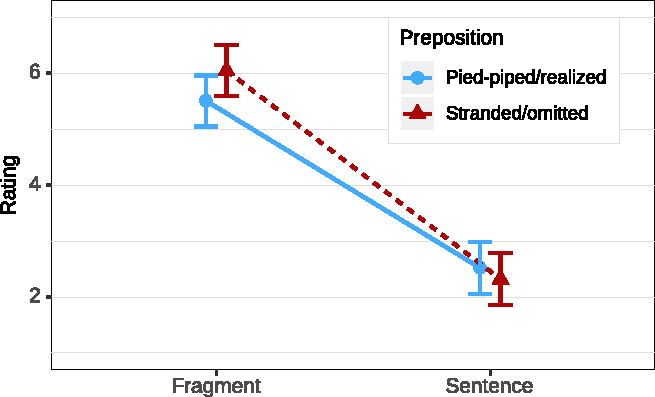
\includegraphics[scale=1]{figures/pst_en_estimates}
 \caption{Mean ratings and 95\% CIs for experiment \ref{exp:pstranding-english}. \label{fig:pstranding-english-estimates}}
\end{figure}

\subsubsection{Results} \label{sec:pstranding-english-results}

Figure \ref{fig:pstranding-english-estimates} provides a summary of the average ratings across conditions. The fragment data show that the omission of the preposition\is{Preposition omission} was slightly more acceptable in English\il{English} \descriptives{6.04}{1.55} than its realization \descriptives{5.5}{1.67}. The sentential left dislocation constructions were heavily degraded across the board no matter whether the preposition was stranded  \descriptives{2.32}{1.43} or pied-piped\is{Pied-piping} \descriptives{2.52}{1.52}. Like in the previous rating studies, the data were analyzed with CLMMs in \texttt{R} following the procedure described in Section \ref{sec:intro-stats}. The full model contained fixed effects for \textsc{Preposition}, \textsc{Sententiality} and \textsc{Position} of the trial in the experiment as well as all two-way interactions thereof. It also contained by-item random intercepts and slopes for \textsc{Preposition}, \textsc{Sententiality} and the interaction thereof and by-subject random intercepts and slopes for \textsc{Preposition}. By-subject random effects for \textsc{Sententiality} were not included, because this IV was tested between subjects. 

\begin{table}
\begin{tabular}{l l l l l l}
\lsptoprule
Predictor & Estimate & SE & $\chi^2$ &  $p$ &  \\   
\midrule
\textsc{Preposition} & 0.258 &  0.138 & \phantom{1}3.83 & \phantom{\textless}0.062 & \marginal \\
\textsc{Sententiality} & 2.997 &  0.322 & 54.94 & \textless \highsig & ***\\
\textsc{Preposition:Sententiality} & 0.499 &  1 & 11.73 & \textless 0.001 & ***\\
\lspbottomrule
\end{tabular}
\caption{Fixed effects in the final CLMM for experiment \ref{exp:pstranding-english}. \label{tab:pstranding-english-estimates}}
\end{table}

The final model (see Table \ref{tab:pstranding-english-estimates}) contains a significant main effect of \textsc{Sententiality} \clmmLR{54.94}{\highsig}, which shows that short answer fragments\is{Fragment, short answer} are rated\is{Acceptability rating task} better than the presumably underlying left dislocation structures. The marginal main effect of \textsc{Preposition} shows that across the board there is no significant difference between P-stranding\is{Preposition stranding}/PP\is{Preposition phrase} fragments and pied-piping\is{Pied-piping}/DP\is{Determiner phrase} fragments \clmmLR{3.38}{0.06}, but the significant interaction between the two predictors \clmmLR{11.73}{0.001} suggests that specifically in the fragment condition DP\is{Determiner phrase} fragments are more acceptable than PP\is{Preposition phrase} fragments.

\subsubsection{Discussion}\largerpage
Experiments \ref{exp:pstranding-german} and \ref{exp:pstranding-english} had the purpose of empirically testing the pattern that the PSG\is{P-Stranding Generalization} predicts with respect to preposition omission\is{Preposition omission} in languages with and without P-stranding\is{Preposition stranding}. Taken together, the experiments empirically confirm the pattern that the PSG\is{P-Stranding Generalization} predicts for German\il{German} and English\il{English} short answer fragments\is{Fragment, short answer}. In German\il{German}, omitting the preposition\is{Preposition omission} in the answer is strongly degraded. In contrast, in English\il{English} both DP\is{Determiner phrase} and PP\is{Preposition phrase} fragments are rated\is{Acceptability rating task} as relatively acceptable, and the omission of the preposition\is{Preposition omission} is actually preferred over its realization. This is in line with the prediction that omitting the preposition\is{Preposition omission} in short answers\is{Fragment, short answer} is degraded in languages that lack P-stranding\is{Preposition stranding}, but at least as acceptable as realizing it in languages that allow for this syntactic operation.

The English\il{English} data from experiment \ref{exp:pstranding-english}, however, also show that all of the left dislocation structures that underlie fragments according to movement and deletion\is{Movement and deletion account} are strongly degraded. Furthermore, there is a significant interaction between \textsc{Sententiality} and \textsc{Preposition}: Contrary to what \citet{merchant2004} predicts, the preference for omitting the preposition\is{Preposition omission} in fragments does not match the acceptability of the corresponding left dislocation structures. This observation can be reconciled with the PSG\is{P-Stranding Generalization} if the exceptional movement\is{Exceptional movement account} version of the theory \citep{weir2014} is assumed, which, however, does not predict a strict parallelism between fragments and left dislocation. Given the discussion on pied-piping\is{Pied-piping} in the introduction to this section, \citet{weir2014} would have to explain pied-piping\is{Pied-piping} as the result of a ban on extracting PPs\is{Preposition phrase} which are the complement of a preposition \citep{abels2003, abels2012}. In that case, fronting the complete PP is the only way to evacuate focused constituents from the ellipsis site \citep{heck2008}.

The PSG\is{P-Stranding Generalization} does not explain why omitting the preposition\is{Preposition omission} is preferred in my materials in English\il{English}. A possible reason for this could be that this is due to P-stranding\is{Preposition stranding} in the question. This could either reflect a general preference for omitting the preposition\is{Preposition omission} whenever it is given in the question (this is not possible in German\il{German}), or be an effect of question-answer congruence, as already hinted at above. I return to this question in experiment \ref{exp:pstranding-production}.

The data also have implications for the other theories of fragments discussed in Chapter \ref{sec:chapter-theories}. For the nonsentential and in situ deletion\is{In situ deletion account} accounts, the challenge is to provide an explanation for the data from experiments \ref{exp:pstranding-german} and \ref{exp:pstranding-english} that does not rely on movement. Experiments \ref{exp:pstranding-defaultcase} and \ref{exp:pstranding-production} test such non-movement accounts of the preposition omission\is{Preposition omission} data, which are based on case checking\is{Case feature} (experiment \ref{exp:pstranding-defaultcase}) and a nonsyntactic parallelism between question and answer (experiment \ref{exp:pstranding-production}). Empirical evidence for either of these hypotheses would leave movement-based accounts\is{Movement and deletion account} without an explanatory benefit over the simpler in situ deletion\is{In situ deletion account} account.

The results also tentatively speak against the claim by \citet{bergen.goodman2015}\is{Ungrammaticality of fragments} that fragments are ungrammatical. Since the missing preposition\is{Preposition omission} (as well as the other omitted material) was unambiguously retrievable from the question, their account does not predict a crosslinguistic difference between English\il{English} and German\il{German} with respect to the acceptability of DP\is{Determiner phrase} fragments. In fact, if all that matters is whether the hearer can retrieve the omitted material, preposition omission might be expected to be \textit{more} acceptable in German\il{German} than in English\il{English}, because the German\il{German} DP\is{Determiner phrase} has prepositional case\is{Prepositional case} marking which restricts the set of possible prepositions. For instance, a hearer who encounters a dative\is{Dative case} DP\is{Determiner phrase} fragment can figure out that the missing preposition must be among those requiring dative\is{Dative case}, whereas such a cue is not available in English\il{English}. This prediction is therefore disconfirmed by the data. This argument of course does not neglect the relevance of information-theoretic\is{Information theory} and processing-based\is{Processing effort} factors to the acceptability and usage of fragments. The experiments in Chapter \ref{sec:chapter-infotheory-experiments} show that predictability plays an important role in the choice between omitting and realizing words.

\refstepcounter{expcounter}\label{exp:pstranding-defaultcase}
\subsection{Experiment \ref{exp:pstranding-defaultcase}: Preposition omission and case}
\label{sec:pstranding-defaultcase}
\subsubsection{Background}
Experiment \ref{exp:pstranding-defaultcase} investigates how acceptable\is{Acceptability rating task} nominative\is{Nominative case} DP\is{Determiner phrase} short answers\is{Fragment, short answer} are as compared to PP\is{Preposition phrase} and prepositional case\is{Prepositional case}-marked DP\is{Determiner phrase} short answers\is{Fragment, short answer} in German\il{German}. This tests two predictions by movement and deletion\is{Movement and deletion account} and the nonsentential account\is{Nonsentential account} of fragments:  First, movement and deletion\is{Movement and deletion account} predicts that nominative\is{Nominative case} DP\is{Determiner phrase} fragments are grammatical as answers to PP\is{Preposition phrase} questions when they can be derived from a cleft\is{Cleft}. Second, the nonsentential account\is{Nonsentential account} also predicts nominative\is{Nominative case} fragments to be acceptable in such contexts: Nominative is the default case\is{Default case} in German\il{German} and does not need to be checked by a preposition. Under both of these lines of reasoning it is expected that PP\is{Preposition phrase} fragments are grammatical, that nominative\is{Nominative case} DP\is{Determiner phrase} fragments are relatively acceptable because they are grammatical, and that prepositional case\is{Prepositional case}-marked DP\is{Determiner phrase} fragments are ungrammatical. According to movement and deletion\is{Movement and deletion account}, their derivation involves ungrammatical P-stranding\is{Preposition stranding}  and according to the nonsentential account\is{Nonsentential account}, prepositional case\is{Prepositional case}-marked DP\is{Determiner phrase} fragments contain a strong uninterpretable case feature\is{Case feature}.

\citet{barton.progovac2005} do not explicitly discuss the status of the PSG\is{P-Stranding Generalization} as evidence for movement, but they observe a crosslinguistic difference between English\il{English} and Serbian\il{Bosnian/Croatian/Serbian} with respect to the possibility of omitting prepositions \is{Preposition omission} in telegraphese utterances. At the example of \Next, \citet[88,89]{barton.progovac2005} show that prepositions can be omitted in English\il{English} sentences like \Next[a], whereas they are obligatory in the Serbian\il{Bosnian/Croatian/Serbian} example \Next[b]. As Serbian\il{Bosnian/Croatian/Serbian} lacks P-stranding\is{Preposition stranding} \citep[667--668]{merchant2004}, this pattern resembles the PSG\is{P-Stranding Generalization}. However, preposition omission\is{Preposition omission} occurs in situ in \Next, so the pattern cannot be explained by a restriction\is{Movement restriction} on extracting a DP\is{Determiner phrase} out of the PP\is{Preposition phrase}, like \citet{merchant2004} proposes for preposition omission\is{Preposition omission} in short answers\is{Fragment, short answer}. Whatever blocks the omission in Serbian\il{Bosnian/Croatian/Serbian} must be independent from movement. Note also that these data are highly relevant to the in situ deletion\is{In situ deletion account} account, because they show that omitting a preposition\is{Preposition omission} when the remnant is a prepositional case\is{Prepositional case}-marked DP\is{Determiner phrase} can be ruled out even in situ.

\ex. \a. Please pick me up (at) Summerside Motel.
\bg. Vidimo se *(na) JFK aerodrom-u.\\
see.\textsc{1pl} Reflexive \phantom{*(}on JFK airport.\textsc{loc}\\
\trans{See you (at) JFK airport.}

\citet{barton.progovac2005} argue that the independent factor that blocks the omission of the preposition\is{Preposition omission} in Serbian\il{Bosnian/Croatian/Serbian} is case checking\is{Case feature}: English\il{English} case features\is{Case feature} are weak and can remain unchecked, whereas Serbian\il{Bosnian/Croatian/Serbian} has strong case features\is{Case feature}, which must be checked. According to \citeauthor{barton.progovac2005}, the strength of Serbian\il{Bosnian/Croatian/Serbian} case features is evidenced by the morphological marking of case. Note that this requires an analysis of prepositional\is{Prepositional case} locative case in \Last[b] as structural case\is{Structural case}, because inherent\is{Inherent case} case can always remain unchecked according to the nonsentential account\is{Nonsentential account}. I return to this issue below. In contrast to the ungrammatical \Last[b], \citeauthor{barton.progovac2005} observe that the preposition can be omitted\is{Preposition omission} in Serbian\il{Bosnian/Croatian/Serbian} when the DP\is{Determiner phrase} appears in nominative\is{Nominative case} case, which they argue is default case\is{Default case} \Next. As they pursue a nonsentential account\is{Nonsentential account}, they do not assume that examples like \Next or the English\il{English} \Last[a] involve the deletion of the preposition, but analyze the noun phrase\is{Noun phrase} as a bare NP\is{Noun phrase}, which simply appears in default case\is{Default case}. Omitting the preposition\is{Preposition omission} is licensed because it is recoverable ``from the verb and the rest of the clause'' \citep[89]{barton.progovac2005}.\largerpage[2]

\exg. Vidimo se, JFK aerodrom.  \\
see.\textsc{1pl} Reflexive  JFK airport.\textsc{nom}\\
\trans{See you, JFK airport.} \exsourceraised{\citep[89]{barton.progovac2005}}

\begin{sloppypar}\noindent
If the contrast in \LLast could be generalized crosslinguistically, these data would provide a non-movement explanation for the PSG\is{P-Stranding Generalization}: The preposition cannot be omitted\is{Preposition omission} in languages that have prepositional case\is{Prepositional case} marking, but it can in languages that do not, because prepositional case\is{Prepositional case} must be checked by an overt preposition. Interestingly, most of the languages that lack P-stranding\is{Preposition stranding} according to \citet{merchant2004}, such as German\il{German} and Slavonic languages, have prepositional case\is{Prepositional case} marking.%
%
\footnote{This is not true for all of the languages that allow DP\is{Determiner phrase} short answers\is{Fragment, short answer} to PP\is{Preposition phrase} questions according to \citet{merchant2004}. Icelandic\il{Icelandic} has morphological case marking and still allows for P-stranding\is{Preposition stranding} and omission in short answers\is{Fragment, short answer}, whereas Hebrew\il{Hebrew} has no morphological case marking and no P-stranding\is{Preposition stranding}. In the case of Hebrew\il{Hebrew} this could be due to the incorporation of the preposition by the noun. %
}\afterfn%
%
I anticipated above that this reasoning requires that prepositional case\is{Prepositional case} is analyzed as structural case.%
% 
\footnote{
This has been explicitly claimed by \citet[24]{dendikken2013}. In his minimalist\is{Minimalist program} approach, prepositional case\is{Prepositional case} is checked by the head of a functional projection in the PP\is{Preposition phrase} layer and not by P itself. The layer relies crucially on the presence of the preposition, hence prepositional case\is{Prepositional case} is licensed only if the preposition is present.}\afterfn%
%
At least in German\il{German}, this seems to be correct. In Section \ref{sec:theories-predictions-case} I defined structural case\is{Structural case} as a purely linguistic device that makes no significant contribution to meaning. In contrast, inherent\is{Inherent case} case makes such contributions by encoding a specific \texttheta-role. Whether a specific prepositional case\is{Prepositional case} encodes aspects of meaning is an empirical issue. In German\il{German} for instance, there is a tendency for dative\is{Dative case} prepositional case\is{Prepositional case} to mark locations or sources and for accusative\is{Accusative case} to mark goals \citep[8]{zwarts2005}. Still, this relationship is not systematic, because a dative\is{Dative case} DP\is{Determiner phrase} can encode a source \Next[a] as well as a goal \Next[b] and location \Next[c] depending on the preposition it appears with. Taken together, just like I argued in Section \ref{sec:theories-predictions-case} for accusative\is{Accusative case}, prepositional case behaves rather like structural than like inherent\is{Inherent case} case, because it is not strictly associated with a specific \texttheta-role. Even though in German the dative prepositional case\is{Dative case} might be likely to mark the location of an event, it does not always convey this aspect of meaning, unlike inherent\is{Inherent case} dative\is{Dative case}, which marks the recipient.\end{sloppypar}\largerpage

\ex. \ag. Er rannte aus dem Park.\\
he ran  out the.\textsc{dat} park\\
\trans{He ran out of the park.}  \exsourceraised{\citep[5]{zwarts2005}}
\bg. Er rannte zum Park.\\
he ran to-the.\textsc{dat} park\\
\trans{He ran to the park.} \exsourceraised{\citep[5]{zwarts2005}}
\cg. Er spielte im Park Badminton.\\
he played in-the.\textsc{dat} park badminton\\
\trans{He played badminton in the park.}

If prepositional case\is{Prepositional case} is thus not semantically interpretable, it requires an overt licensor just like other instances of structural case\is{Structural case} do in \citeauthor{barton.progovac2005}'s framework.%
%
\footnote{\citet[342]{progovac.etal2006} argue that a specific prepositional case\is{Prepositional case}, like accusative\is{Accusative case} in the Serbian\il{Bosnian/Croatian/Serbian} example \Next, is acceptable in fragments if it can also be used as inherent\is{Inherent case} case encoding a \texttheta-role. Nevertheless, non-prepositional accusative\is{Accusative case} is associated with the \textsc{Patient} \texttheta-role, so that the fragment is assigned a misleading interpretation if the preposition is omitted\is{Preposition omission}. 

\ex. \ag. Na čega je Stefan seo?\\
	      on what did Stefan sit\\
	      \trans{What did Stefan sit on?} \exsourceraised{\citep[342]{progovac.etal2006}}
	 \bg. *(Na) stolicu.\\
	      on chair.\textsc{acc}\\
	      \trans{(On) a chair.}
	      
Note however that this accounts only for prepositional case\is{Prepositional case} that is otherwise inherent\is{Inherent case}, such as dative\is{Dative case} and genitive\is{Genitive case} in German\il{German}. As I argued above in Section \ref{sec:theories-predictions-case}, there are good reasons not to analyze German\il{German} accusative\is{Accusative case} as inherent\is{Inherent case} (possibly in contrast to Serbian\il{Bosnian/Croatian/Serbian}), so that this explanation does not immediately concern my experiments.}\afterfn%
%
The nonsentential account\is{Nonsentential account} can hence explain at least a large part of the preposition omission\is{Preposition omission} data without assuming unarticulated linguistic structure, actually \textit{because} of the assumption that there is no unarticulated material in fragments that could check the uninterpretable case features\is{Case feature}.%
% 
\footnote{\citet{barton.progovac2005} do not discuss sluicing\is{Sluicing}, therefore it remains open whether they would make a similar prediction for the phenomenon that originally motivated the PSG\is{P-Stranding Generalization}.}\afterfn%
%

Experiment \ref{exp:pstranding-defaultcase} tests this prediction by collecting acceptability ratings\is{Acceptability rating task} for three types of short answer fragments\is{Fragment, short answer} in German\il{German}: PP\is{Preposition phrase} fragments, prepositional case\is{Prepositional case}-marked DP\is{Determiner phrase} fragments and default case-marked DP\is{Determiner phrase} fragments. German\il{German} does not allow for P-stranding\is{Preposition stranding}, it has prepositional case\is{Prepositional case} marking (accusative\is{Accusative case}, dative\is{Dative case} and genitive\is{Genitive case}) as well as nominative\is{Nominative case} default case that never appears as prepositional case\is{Prepositional case}. The nonsentential account\is{Nonsentential account} makes in principle the same predictions as the PSG\is{P-Stranding Generalization} does for PP\is{Preposition phrase} and prepositional case\is{Prepositional case}-marked DP\is{Determiner phrase} fragments: PP\is{Preposition phrase} fragments \Next[a] are expected to be acceptable and prepositional case\is{Prepositional case}-marked DP\is{Determiner phrase} fragments \Next[b] to be degraded. However, the theories disagree on the acceptability of default case DP\is{Determiner phrase} fragments \Next[c]. The nonsentential account\is{Nonsentential account} predicts them to be acceptable, because default case does not need to be checked and the preposition can be easily retrieved from the question. Any sentential account however predicts in principle that the form of the answer matches that of the question, so nominative\is{Nominative case} DP\is{Determiner phrase} fragments will be degraded as compared to PP\is{Preposition phrase} fragments. 

\exg.  Für wen ist das Päckchen?\label{ex:pstranding-defaultcase-sample-item}\\
     for who.\textsc{acc} is the package\\
    \trans{For whom is the package?}
    \ag. Für meinen Vater.\\
     for my.\textsc{acc} father\\
     \trans{For my father.}\exsourceraised{PP}
\bg. Meinen Vater. \\
     my.\textsc{acc} father\\
     \trans{My father.}\exsourceraised{DP, prepositional case}\is{Prepositional case}
 \cg. Mein Vater. \\
     my.\textsc{nom} father\\
     \trans{My father.}\exsourceraised{DP, nominative\is{Nominative case} case}

This does neither imply that the nonsentential account\is{Nonsentential account} predicts nominative\is{Nominative case} DP\is{Determiner phrase} fragments to be as acceptable as PP\is{Preposition phrase} fragments, nor that sentential accounts predict nominative\is{Nominative case} DP\is{Determiner phrase} fragments to be as degraded as prepositional case\is{Prepositional case}-marked DP\is{Determiner phrase} fragments. As for the nonsentential account\is{Nonsentential account}, \citet{progovac.etal2006} argue that even though default case\is{Default case} DP\is{Determiner phrase} fragments are grammatical, they might still be dispreferred for pragmatic reasons. They exemplify this with  \Next, for which they claim that nominative\is{Nominative case} is degraded, because the speaker could have chosen the matching accusative\is{Accusative case} fragment (recall that \citet{progovac.etal2006} claim that the Serbian\il{Bosnian/Croatian/Serbian} accusative\is{Accusative case} is inherent\is{Inherent case} case). Therefore, nominative\is{Nominative case} DP\is{Determiner phrase} fragments might be worse than PP\is{Preposition phrase} fragments, but the nonsentential account\is{Nonsentential account} predicts them to be better than structural case\is{Structural case}-marked DP\is{Determiner phrase} fragments, which are blatantly ungrammatical.

\ex. \ag. Koga je Ana posetila?\\
who.\textsc{acc} is Ana visited \\
\trans{Who did Ana visit?}\exsourceraised{\citep[340]{progovac.etal2006}}
\bg. Vera!\\
Vera.\textsc{nom}\\

In contrast, according to the sentential account, the acceptability of a fragment depends on the availability of a matching antecedent. For instance, nominative\is{Nominative case} would be acceptable if subjects formed a (highly marked) cleft\is{Cleft}ed structure, that requires nominative\is{Nominative case} on the DP\is{Determiner phrase}, as implicit antecedent. Anticipating the results of the experiment,  nominative\is{Nominative case} is rated\is{Acceptability rating task} as even worse than accusative\is{Accusative case}, so this theoretical possibility does not need to be further discussed.

\exg. Es ist mein Vater, für den das Päckchen ist.\\
      it is my.\textsc{nom} father for who.\textsc{acc} the package is\\
      \trans{It's my father, for whom the package is.}

\subsubsection{Materials}
The stimuli were identical to those used in experiment \ref{exp:pstranding-german} except for the additional nominative\is{Nominative case} DP\is{Determiner phrase} fragment condition. The three conditions are exemplified in \ref{ex:pstranding-defaultcase-sample-item} above. As compared to experiment \ref{exp:pstranding-german}, one further item was added in order to present each of the three conditions equally often to the participants.

\subsubsection{Procedure}
The experiment was conducted over the Internet using the LimeSurvey presentation software and completed by 48 participants recruited on the \textit{clickworker} crowdsourcing platform. Each participant was paid \currencyEuro{4.00} for their participation. Subjects were asked to rate the naturalness of the italicized short answer fragment\is{Fragment, short answer} in the context of the question on a 7-point Likert scale (7 = fully natural). Materials were mixed with 24 items from experiment \ref{exp:scripts-rating} and 44 fillers. Both the materials from experiment \ref{exp:scripts-rating} and the fillers resembled the items of experiment \ref{exp:pstranding-defaultcase} in having a context story and an italicized target utterance which subjects rated\is{Acceptability rating task}. Subjects were assigned to one of six lists, to which materials were allocated by a Latin square so that each subject saw each token set only once and each condition equally often. Each two of these lists contained the same materials for experiment \ref{exp:pstranding-defaultcase}, but differed with respect to the materials from experiment \ref{exp:scripts-rating}. All lists were presented in an individually pseudo-randomized order that ensured that no two items or fillers of the same category immediately followed each other. Three subjects rated\is{Acceptability rating task} more than the previously established threshold of two out of five ungrammatical controls as natural (6 or 7 points) and thus were excluded from further analysis.

\subsubsection{Results} 
Table \ref{tab:p-case-means} summarizes the ratings for the three conditions. The ratings for PP\is{Preposition phrase} and prepositional case\is{Prepositional case}-marked DP\is{Determiner phrase} fragments replicate the previous studies. Nominative\is{Nominative case} DP\is{Determiner phrase} fragments are perceived as even less acceptable than prepositional case\is{Prepositional case}-marked DP\is{Determiner phrase}s.

\begin{table}
 \begin{tabular}{l l l l}
 \lsptoprule
  Condition &  Exp. \ref{exp:pstranding-defaultcase} & Exp. \ref{exp:pstranding-german} & \citet{merchant.etal2013}\\
 \midrule
 PP\is{Preposition phrase} & 6.31 (1.18) & 6.61 (0.99)& 5.99 (1.64)\\
DP\is{Determiner phrase}, Structural case & 4.81 (1.99)&4.42 (2.05)& 4.76 (2.03)\\
DP\is{Determiner phrase}, Nominative\is{Nominative case} & 3.57 (1.96)& -- & -- \\
\lspbottomrule
 \end{tabular}
  \caption{Mean ratings (standard deviation) by condition in experiment \ref{exp:pstranding-defaultcase}, in experiment \ref{exp:pstranding-german} and in the P-stranding study by \citet{merchant.etal2013}\label{tab:p-case-means}. \textit{Structural case} refers to prepositional case in experiment \ref{exp:pstranding-defaultcase} and accusative in the other two studies.}
 \end{table}

The data were analyzed with CLMMs in \texttt{R} following the procedure described in Section \ref{sec:intro-stats}. In this case, the procedure slightly differed from that applied to previous studies, because the IV was a nominal-scaled factor with three levels. The likelihood ratio tests used for model selection only allow for the comparison of two models containing or lacking a factor and but not for pairwise comparisons between the individual levels. Therefore, I created two subsets from the complete data set in order to compare the factor levels  pairwise. I first compared only the PP\is{Preposition phrase} to the prepositional case\is{Prepositional case}-marked DP\is{Determiner phrase} fragments, thus replicating experiment \ref{exp:pstranding-german}. Then I tested whether the nominative\is{Nominative case} and prepositional case\is{Prepositional case}-marked DP\is{Determiner phrase} fragments differed significantly in acceptability\is{Acceptability rating task} by analyzing these conditions only. This procedure allows for pairwise comparisons between factor levels and not only for testing whether including a factor as a whole improves model fit. For both subsets I started with a full model containing fixed effects for \textsc{FragmentType}, the \textsc{Position} of the trial in the experiment and their interaction and by-item and by-subject random intercepts and random slopes for each predictor. The final models (see Tables \ref{tab:pst-case-estimates-pp-str} and \ref{tab:pst-case-estimates-str-def}) show that all contrasts between the levels of \textsc{FragmentType} are significant. PP\is{Preposition phrase}s are rated\is{Acceptability rating task} significantly better than case-marked DP\is{Determiner phrase}s \clmmLR{29.18}{\highsig} and nominative\is{Nominative case} case-marked DP\is{Determiner phrase}s are even worse than prepositional case\is{Prepositional case}-marked DP\is{Determiner phrase}s \clmmLR{15.37}{\highsig}. In the model that compared PP\is{Preposition phrase}s to prepositional case\is{Prepositional case}-marked DP\is{Determiner phrase} fragments there was also a significant \textsc{Position} effect, which did not interact with \textsc{FragmentType}.

\begin{table}
\begin{tabular}{l c c c c c}
\lsptoprule
Predictor & Estimate & SE & $\chi^2$ &  $p$ &  \\   
\midrule
\textsc{FragmentType} & 2.58 & 0.423 &  15.37 & \textless \highsig& ***\\
\textsc{Position} &  0.01 & 0.004 &  \phantom{1}4.34  &  \textless 0.05& *\\
\lspbottomrule
\end{tabular}
 \caption{Fixed effects in the final model comparing PP fragments to prepositional case-marked DP fragments.\label{tab:pst-case-estimates-pp-str}}
\end{table}

\begin{table}
\begin{tabular}{l c c c c c}
\lsptoprule
Predictor & Estimate & SE & $\chi^2$ &  $p$ &  \\   
\midrule
\textsc{FragmentType} & 1.838 & 0.414 & 29.18 & \textless \highsig &***\\
\lspbottomrule
\end{tabular} 
\caption{Fixed effects in the final model comparing prepositional case-marked DP fragments to nominative DP fragments.\label{tab:pst-case-estimates-str-def}}
\end{table}

\subsubsection{Discussion}
Experiment \ref{exp:pstranding-defaultcase} tested whether nominative\is{Nominative case} DP\is{Determiner phrase} fragments are more acceptable than prepositional case\is{Prepositional case}-marked DP\is{Determiner phrase} fragments, and how they are rated\is{Acceptability rating task} in comparison to PPs\is{Preposition phrase}. Both the nonsentential account\is{Nonsentential account} \citep{barton.progovac2005} and the movement and deletion\is{Movement and deletion account} account predict a preference for nominative\is{Nominative case} DP\is{Determiner phrase}s over case-marked ones, but for independent reasons. According to the nonsentential account\is{Nonsentential account}, prepositions can be omitted\is{Preposition omission} in short answer fragments\is{Fragment, short answer} only if they are not required for checking prepositional case\is{Prepositional case}. The nonsentential account\is{Nonsentential account} predicts fragments in nominative\is{Nominative case} default case to be acceptable under such circumstances. According to the movement and deletion\is{Movement and deletion account} account, DP\is{Determiner phrase} short answers might be grammatical as answers to PP questions in German\il{German} when they can be derived from a cleft\is{Cleft}. In that case, the DP\is{Determiner phrase} must exhibit nominative\is{Nominative case} case morphology. 

The experiment disconfirms these predictions: Nominative\is{Nominative case} DP\is{Determiner phrase} fragments are significantly less acceptable than prepositional case\is{Prepositional case}-marked ones. PP\is{Preposition phrase} short answers\is{Fragment, short answer} are even more strongly preferred than prepositional case\is{Prepositional case}-marked DP\is{Determiner phrase}s. This finding challenges the cleft\is{Cleft}-based analysis of apparent preposition omission\is{Preposition omission} under ellipsis in languages that lack P-stranding\is{Preposition stranding}. In a language with overt case marking, like German\il{German}, such an account predicts that DP\is{Determiner phrase} fragments derived from clefts\is{Cleft} by ellipsis appear in nominative, just like in the corresponding full sentences. Even though the movement and deletion\is{Movement and deletion account} account does not predict that the resulting nominative DP\is{Determiner phrase} fragments are as acceptable as PP\is{Preposition phrase}s (they might be degraded for pragmatic reasons), they are expected to be more acceptable than prepositional case\is{Prepositional case}-marked DP\is{Determiner phrase}s, which it analyzes as being derived only by ungrammatical P-stranding\is{Preposition stranding}. This prediction is clearly disconfirmed by the experiment, since this predicted acceptability\is{Acceptability rating task} pattern is inverted in the data.

From the perspective of the nonsentential account\is{Nonsentential account}, the contrast to the English\il{English} data from experiment \ref{exp:pstranding-english}, which revealed a preference for preposition omission\is{Preposition omission}, is particularly striking. If the explanation for the English\il{English} pattern is that the preposition can be omitted\is{Preposition omission} because it is given in the question and the resulting nominative\is{Nominative case} DP\is{Determiner phrase} fragment does not require case checking\is{Case feature}, the same pattern is expected for German\il{German} default case\is{Default case} (nominative\is{Nominative case}) DP\is{Determiner phrase} fragments. Therefore, experiment \ref{exp:pstranding-defaultcase} strongly suggests that the nonsentential case checking\is{Case feature} account should be rejected. Sentential accounts predict connectivity effects\is{Case connectivity} between question and answer, and consequently are in line with the preference for realizing the preposition in the answer as well. 

The gradual acceptability\is{Acceptability rating task} cline between the three short answer\is{Fragment, short answer} types is in line with the idea that fragments are ungrammatical but can be interpreted after applying a probabilistic repair mechanism, as \citet{bergen.goodman2015}\is{Ungrammaticality of fragments} suggest. The prepositional case\is{Prepositional case}-marked DP\is{Determiner phrase} fragments are clearly dispreferred in all three experiments and are therefore degraded in the context of PP\is{Preposition phrase} questions in German\il{German}. Nonetheless, prepositional case\is{Prepositional case} can function as a probabilistic cue that points toward the preposition that is missing. Since prepositional case\is{Prepositional case} is determined by the preposition, processing a dative\is{Dative case} DP\is{Determiner phrase} will restrict the range of possible prepositions to those requiring dative\is{Dative case}. Nominative\is{Nominative case} DP\is{Determiner phrase} fragments could be rated\is{Acceptability rating task} worse because they lack this cue. Under this perspective, both case-marked and default case\is{Default case} DP\is{Determiner phrase} fragments are ungrammatical, because they lack an appropriate antecedent. The acceptability difference between these ungrammatical utterances could be explained by the effort\is{Processing effort} required to figure out which part of the utterance is missing. However, the comparison between English\il{English} and German\il{German} in experiments \ref{exp:pstranding-german} and \ref{exp:pstranding-english} shows that the recoverability of the preposition cannot be the whole story. Its omission\is{Preposition omission} is less acceptable in German\il{German} despite the fact that English\il{English} lacks prepositional case\is{Prepositional case} as a cue toward in the omitted preposition\is{Preposition omission}. Consequently, the preference for prepositional case\is{Prepositional case} in comparison to default case\is{Default case} might be due to differences in recoverability of the omitted preposition\is{Preposition omission}, but the inverted preference for DP\is{Determiner phrase} and PP\is{Preposition phrase} short answer\is{Fragment, short answer}s between German\il{German} and English\il{English} must receive a different explanation. 

Taken together, experiment \ref{exp:pstranding-defaultcase} disconfirms the case checking\is{Case feature}-based account that follows from the discussion on preposition omission\is{Preposition omission} in \citet{barton.progovac2005}. The experiment also showed that nominative\is{Nominative case} DP\is{Determiner phrase} fragments, which might be derived from cleft\is{Cleft} structures according to movement and deletion\is{Movement and deletion account} are more strongly degraded than presumably ungrammatical DP\is{Determiner phrase}s in prepositional case\is{Prepositional case}. The relative acceptability of these DP\is{Determiner phrase}s as compared to nominative\is{Nominative case} ones, which all of the theories can derive, suggests that they might not be fully ungrammatical but dispreferred for independent reasons. Experiment \ref{exp:pstranding-production} addresses this issue.

\refstepcounter{expcounter}\label{exp:pstranding-production}
\subsection{Experiment \ref{exp:pstranding-production}: Question-answer parallelism}
\label{sec:pstranding-production}

\subsubsection{Background}
\label{sec:pstranding-production-background}

Experiment \ref{exp:pstranding-production} tests the hypothesis that the availability of P-stranding\is{Preposition stranding} and of preposition omission\is{Preposition omission} in a language often cooccur due to a nonsyntactic relationship between question and answer. If this hypothesis were confirmed, the data that \citet{merchant2004} interprets as evidence for movement\is{Movement and deletion account} in fragments could be explained without assuming that movement is required as an explanatory link between the acceptability of fragments and the availability of P-stranding\is{Preposition stranding}.

\is{Fragment, short answer|(}\is{Preposition omission|(}The data discussed so far are in line with the PSG\is{P-Stranding Generalization}: Experiments \ref{exp:pstranding-german} and \ref{exp:pstranding-english} confirm its predictions for English\il{English} and German\il{German} and experiment \ref{exp:pstranding-defaultcase} rules out the alternative nonsentential account\is{Nonsentential account} based on case checking\is{Case feature}. However, parallelisms between fragments and movement constructions support the movement and deletion\is{Movement and deletion account} account only if derivationally simpler theories, like the nonsentential\is{Nonsentential account} and in situ deletion\is{In situ deletion account} accounts, cannot explain the data as well. In the case of the PSG\is{P-Stranding Generalization}, there are at least three possible explanations for the data: First, as \citet{merchant2004} argues, they could of course evidence a genuine movement restriction\is{Movement restriction}. Second, there could be an independent factor that blocks the omission of the preposition\is{Preposition omission} in languages that disallow P-stranding\is{Preposition stranding}. The nonsentential case checking\is{Case feature} hypothesis that I tested in the previous section is an example for this line of reasoning. Even though I rejected this explanation, the impossibility of omitting prepositions\is{Preposition omission} in German\il{German} (as compared to English\il{English}) in in situ contexts might still evidence such a different independent factor other than the one I tested in experiment \ref{exp:pstranding-defaultcase}.%
%
\footnote{For instance, \citet[21]{zwarts2005} claims that preposition and case are ``not two semantically independent elements'' in German\il{German}, but that they are interpreted together. Another such factor could be crosslinguistic differences with respect to feature percolation\is{Feature percolation}. If a focus feature percolated from the DP\is{Determiner phrase} to PP\is{Preposition phrase} obligatorily in German\il{German} but not in English\il{English}, e.g. due to PP\is{Preposition phrase}-internal movement operations required for case checking\is{Case feature}, the in situ deletion\is{In situ deletion account} account could explain why the omission of the preposition\is{Preposition omission} is blocked in languages that do not allow for P-stranding\is{Preposition stranding}.}\afterfn%
% 

A third possibility, which experiment \ref{exp:pstranding-production} explores, is that there is no structural difference between English\il{English} and German\il{German} PPs\is{Preposition phrase} that blocks the omission of the preposition\is{Preposition omission} in fragments, but that the form of the \textit{wh}-phrase in the question constrains that of the answer\is{Fragment, short answer}: If the preposition is pied-piped\is{Pied-piping} in the question, it must be realized in short answers\is{Fragment, short answer}, and if it is stranded in the question, it is omitted\is{Preposition omission} in the answer\is{Fragment, short answer}. From this perspective, preposition omission\is{Preposition omission} in German\il{German} short answers\is{Fragment, short answer} is not blocked by properties of the answer\is{Fragment, short answer}, but dispreferred because of the impossibility of stranding\is{Preposition stranding} the preposition in the question. In principle, both forms of the answer\is{Fragment, short answer} are possible, but one of them is strongly preferred for nonsyntactic reasons.

Experiment \ref{exp:pstranding-production} tests this hypothesis by eliciting answers to questions with pied-piping\is{Pied-piping} and P-stranding\is{Preposition stranding} in a production study\is{Production task} in English\il{English}, which allows for both forms of the answer. If subjects adapt their answer to the question, they must produce a higher ratio of preposition omission\is{Preposition omission} when the preposition is stranded\is{Preposition stranding} the question and realize it more often in the answer when it is pied-piped\is{Pied-piping}.

This raises the question of why such a mechanism would be observed at all. In the theoretical literature, there are at least two possible explanations that predict a nonsyntactic question-answer parallelism: First, a structured propositions account of question semantics \citep{vonstechow1981, reich2002a} relates the focus structure of question and answer. Second, structural persistence \citep{nykiel2017} between question and answer could result from speakers' tendency to reuse structure from previous discourse \citep{levelt.kelter1982, nykiel2017}. 

\subsubsubsection{Structured propositions}
\label{sec:psg-alternatives-structured}

The central idea of the structured propositions account of question-answer parallelism is that the focus structure of the answer is determined by that of the question \citep{reich2002, reich2002a, reich2007}.%
%
\footnote{Note that this might also be expected under a movement and deletion\is{Movement and deletion account} account. However, if it were the case, the prediction of movement and deletion\is{Movement and deletion account} and in situ deletion\is{In situ deletion account} with respect to preposition omission\is{Preposition omission} would be fully aligned: Both theories predict that only words which belong to the focus survive ellipsis, and no matter whether they are previously moved, the outcome is identical. In that case, the PSG\is{P-Stranding Generalization} would not provide genuine evidence for movement. As I showed in Section \ref{sec:pstranding-background-mp}, it does only if the focus structure of pied-piping\is{Pied-piping} and P-stranding\is{Preposition stranding} questions (and the corresponding) answers is identical and pied-piping\is{Pied-piping} occurs because extraction out of PP\is{Preposition phrase} is ungrammatical.}\afterfn%
%
If the preposition in the question is focused, it must also be focused in the answer and therefore cannot be omitted\is{Preposition omission} there. If the preposition is not focused in the question, it also not in the answer, and consequently it can be targeted by ellipsis.%
%
\footnote{See \citet{griffiths2019} for a similar account of the PSG\is{P-Stranding Generalization} data.}\afterfn%
%

\citet{reich2002a} models the semantics of questions as a set of structured propositions, which are sensitive to focus structure \citep{vonstechow1981}. For instance, \citet[82]{reich2002a} defines the semantics of \Next[a] as denoting the set of propositions in \Next[b], which is summarized as \Next[c]. The idea is that, instead of defining the semantics of \Next[a] as a set of unstructured propositions \NNext, the focus, i.e. the \textit{wh}-phrase in \Next, is separated from the background of the question. Congruent answers must match this focus-background structure.

\ex. \a. What did John drive? \hfill \citep[82]{reich2002a}
     \b. $\{\langle Mary's\;red\;convertible, \lambda x.John\;drove\;x \rangle,\\
     \langle Peter's\;Porsche, \lambda x.John\;drove\;x \rangle, \dots\}$
     \c. $\lambda p \exists x [thing'(x)\;\&\;p = \langle x,\;\lambda y.John\;drove\;y\rangle]$
     
\ex. $\lambda x. John\;drove\;x$

\citet{reich2002a} does not address pied-piping\is{Pied-piping}, but in \citet{reich2002} he develops a structured propositions analysis of complex \textit{wh}-phrases. He assumes that the pied-piped\is{Pied-piping} material belongs to the focus in complex \textit{wh}-phrases like \textit{whose book} in \Next[a], whose semantics he defines as \Next[b]. He argues that an answer that does not match this focus-background structure is incongruent, because it is not included in the denotation of the question. Applied to pied-piping\is{Pied-piping} of prepositions, the semantics of a question like \NNext[a] would be defined as \NNext[b], whereas that of the corresponding P-stranding\is{Preposition stranding} question is given in \ref{ex:structural-pstranding}. This requires congruent answers to \NNext and \ref{ex:structural-pstranding} to differ in their focus structure: \ref{ex:structural-pstranding-a-pp} is a congruent answer to \NNext, but \ref{ex:structural-pstranding-a-pst} is not. In the case of a P-stranding question like \ref{ex:structural-pstranding}, the opposite holds.

\ex. \a. Whose book did you read?\hfill\citep{reich2002}
    \b. $\{\langle\langle x, \lambda z . z's book \rangle ,\;\lambda y . you\;read\;y \rangle;\; x \; is \; a \; person\}$
    
\ex. \a. With whom did you talk?
    \b. $\{\langle\langle x, \lambda z . with\; z \rangle ,\;\lambda y.\; you\;talk\;y \rangle;\; x \; is \; a \; person\}$

\ex. \label{ex:structural-pstranding}
\a. Who did you talk with?
    \b. $\{\langle\langle x,\;\lambda y.\; you\;talk\;with\;y \rangle;\; x \; is \; a \; person\}$

\ex. \a. \sout{I talked} [with John]\textsubscript{\textsc{F}}.\label{ex:structural-pstranding-a-pp}
     \b.  \sout{I talked with} [John]\textsubscript{\textsc{F}}.\label{ex:structural-pstranding-a-pst}

The assumption that relatively subtle differences in meaning can impact on the form of fragments has recently been reinforced by \citet{weir2018}. He observes that despite the questions in \Next and \NNext being relatively meaning-equivalent, fragments that do not match the semantics of the \textit{wh}-phrase are heavily degraded.

\ex. \label{ex:weir-qa-ex1}
 Q: How many signals did the machine send? \hfill \citep[1289]{weir2018}
\a.  \a. It sent \textit{two} signals.
\b. ?It sent a signal \textit{twice}.
\z.
\b. \a. \textit{two} (signals).
\b. *\textit{twice}.
\z.

\ex. \label{ex:weir-qa-ex2}
Q: How many times did the machine send a signal? \hfill \citep[1289]{weir2018}
\a. \a. ?It sent \textit{two} signals.
    \b. It sent a signal \textit{twice}.
    \z.
\b.
\a.* \textit{two} (signals).
\b. \textit{twice}.
\z.

The structured propositions approach offers a straightforward explanation for the contrast between German\il{German} and English\il{English} with respect to the acceptability of preposition omission\is{Preposition omission} in fragments. Unlike English\il{English}, German\il{German} lacks P-stranding\is{Preposition stranding} in questions, hence questions always involve pied-piping\is{Pied-piping} and only answers where the complete PP\is{Preposition phrase} is focused are congruent. As the central assumption of the in situ deletion\is{In situ deletion account} account is that focused expressions survive ellipsis, the preposition can never be omitted\is{Preposition omission} in those contexts. With respect to English\il{English}, where both P-stranding\is{Preposition stranding} and pied-piping\is{Pied-piping} are available, the structured propositions approach predicts a relatively strict congruence between the form of the question and that of the answer. As the contrast between \ref{ex:weir-qa-ex1} and \ref{ex:weir-qa-ex2} suggests, there should be a strong preference for the answer to match the form of the question: Pied-piping\is{Pied-piping} questions are expected to require PP\is{Preposition phrase} short answers\is{Fragment, short answer}, whereas P-stranding\is{Preposition stranding} questions require DPs\is{Determiner phrase}.

\subsubsubsection{Structural persistence}
The second account of question-answer parallelism is based on processing\is{Processing effort}. The idea is that both DP\is{Determiner phrase} and PP\is{Preposition phrase} fragments can be derived by the syntax in the context of PP\is{Preposition phrase} questions in English\il{English} and German\il{German}, but that a tendency for speakers to reuse syntactic structure from previous discourse explains why short answer fragments\is{Fragment, short answer} often match the form of the preceding question. This has been proposed by \citet{nykiel2017}, who traces back the observation of a tendency to reuse syntactic structure from previous discourse to \citet{levelt.kelter1982}. \citet{levelt.kelter1982} conducted a series of experiments that investigated how and why speakers reuse structure in the example of the optional omission of prepositions\is{Preposition omission} in Dutch\il{Dutch} questions and answers like \Next, from \citet[80]{levelt.kelter1982}. For this language, they argue that the preposition \textit{aan} `to' can be freely omitted\is{Preposition omission} in the question and the short answer\is{Fragment, short answer} fragment without changing its meaning.

\ex. \ag. (Aan) wie laat Paul zijn viool zien?\\
      to  whom allows Paul his violin see\\
      \trans{Who allows Paul to see his violin?}
      \bg. (Aan) Toos.\\
      to Toos\\
      \trans{Toos.}

Throughout their experiments, \citet{levelt.kelter1982} find an effect of the form of the question on the form of the answer: The preference for omitting the preposition\is{Preposition omission} in the answer is stronger when it is been omitted\is{Preposition omission} in the question and vice versa. Note that \Last does not involve P-stranding\is{Preposition stranding}, but the general idea straightforwardly applies to P-stranding\is{Preposition stranding} data. If speakers reuse the structure given in a P-stranding\is{Preposition stranding} question, they should prefer DP\is{Determiner phrase} fragments, whereas PP\is{Preposition phrase} fragments would be preferred in case of pied-piping\is{Pied-piping} questions. 

This prediction is supported by English\il{English} corpus\is{Corpus} data \citep{nykiel2014, nykiel2017}. \citet{nykiel2017} shows that despite an overall preference for omitting the preposition\is{Preposition omission} in the remnant,%
%
\footnote{\citet{nykiel2017} investigated a more extensive range of antecedents, instead of looking only into question answer pairs. In the case of the latter, the remnant is the short answer\is{Fragment, short answer}.}\afterfn%
%
the rate of DP\is{Determiner phrase} fragments (90\%) is significantly higher when the preposition is stranded\is{Preposition stranding} or omitted\is{Preposition omission} than when the preposition is pied-piped\is{Pied-piping} or appears adjacent to its object (58.8\%). Even though her corpus studies\is{Corpus} are concerned only with English\il{English} data, \citet[41--42]{nykiel2017} argues that her observations for English\il{English} also provide an explanation for the crosslinguistic pattern: If the form of the antecedent (e.g. the PP\is{Preposition phrase} in the question) determines the form of the fragment, DP\is{Determiner phrase} short answers\is{Fragment, short answer} to questions where the \textit{wh}-phrase is the complement of a preposition are only possible when there are DP\is{Determiner phrase} antecedents. In German\il{German} there are never such antecedents because German\il{German} has no P-stranding\is{Preposition stranding}. Consequently, the preposition is never omitted\is{Preposition omission} in the answer.

\subsubsubsection{Predictions of question-answer parallelism}
Both the structured pro\-positions and the structural persistence accounts provide a non-movement explanation for the data that \citet{merchant2001, merchant2004} presents as evidence for the PSG\is{P-Stranding Generalization}. Besides explaining the crosslinguistic data, such an approach predicts that within a language that allows for an alternation between P-stranding\is{Preposition stranding} and pied-piping\is{Pied-piping}, the form of the answer will match that of the question, like \citet{levelt.kelter1982} showed for preposition omission\is{Preposition omission} in Dutch\il{Dutch}.\is{Fragment, short answer|)}

Since the goal of experiment \ref{exp:pstranding-defaultcase} is to investigate whether question-answer parallelism can explain the preposition omission\is{Preposition omission} data without having to assume movement in fragments\is{Movement and deletion account}, the experiment does not need to differentiate between the semantic and the processing accounts. However, the structured propositions account predicts a relatively strict match between question and answer, whereas this relationship might be looser if the structural persistence account is correct. From a semantic perspective, if focusing the preposition in the question blocks its omission\is{Preposition omission} in the answer, the form of the question would strictly determine that of the answer. The tendency to reuse structure might interact with and be overridden by other constraints, such as the tendency to be brief and to omit redundant material.%
%
\footnote{See Section \ref{sec:infotheory-uid} for discussion.}\afterfn%
%
The conclusions on this issue will only be tentative.

In contrast to question-answer parallelism, the movement and deletion\is{Movement and deletion account} account does not necessarily predict a correlation between the form of the question and the answer: As I discussed above, if the alternation between DP\is{Determiner phrase} and PP\is{Preposition phrase} short answers\is{Fragment, short answer} is traced back to different focus structures, it does not provide evidence specifically for movement\is{Movement and deletion account}. Consequently, movement and deletion\is{Movement and deletion account} implies that P-stranding\is{Preposition stranding} and pied-piping\is{Pied-piping} questions do not differ with respect to their focus structure. It is important to note that a syntactic theory like the movement and deletion\is{Movement and deletion account} account does not conflict with the assumption of processing constraints\is{Processing effort}, like the structural persistence account. Processing constraints can determine the choice for a particular utterance when grammar allows for various options. However, if an independently evidenced processing constraint can explain the data that the syntactic theory was designed to account for, this syntactic theory yields no explanatory benefit over simpler theories. In that case, the preposition omission\is{Preposition omission} data would lose their status as evidence for movement in fragments\is{Movement and deletion account}.\is{Preposition omission|)}

\subsubsubsection{Approach}
Experiment \ref{exp:pstranding-production} uses a production task\is{Production task} to investigate whether subjects adapt answers to the form of the question. I conducted the study in English\il{English}, which allows for both P-stranding\is{Preposition stranding} and pied-piping\is{Pied-piping}. There is some previous experimental evidence that points into this direction: The corpus studies\is{Corpus} by \citet{nykiel2014, nykiel2017} and the experiments by \citet{levelt.kelter1982} suggest that there is question-answer parallelism, but \citet{levelt.kelter1982} investigate a related yet different phenomenon and \citet{nykiel2014, nykiel2017} considers very diverse antecedents and remnants, such as interrogative fragments and elliptical questions. An experimental study allows for controlling this variance and for testing only pied-piping\is{Pied-piping} and P-stranding\is{Preposition stranding} questions, which are the relevant antecedents given the above discussion on question-answer parallelisms.

In the experiment, subjects read a context story followed by a question with a stranded\is{Preposition stranding} \Next[a] or a pied-piped\is{Pied-piping} \Next[b] preposition and are asked to produce a natural answer to that question. Question-answer parallelism predicts a (relatively) higher rate of DP\is{Determiner phrase} fragments for P-stranding\is{Preposition stranding} questions \Next[a] and a higher rate of PP\is{Preposition phrase} fragments for questions with pied-piping\is{Pied-piping} \Next[b]. 

\ex. Molly and Cooper are colleagues and talk about football during a break. Because this evening there is an important match, Cooper asks Molly:
\a. Who are you rooting for? \hfill P-stranding\is{Preposition stranding}
\b. For whom are you rooting? \hfill Pied-piping\is{Pied-piping}

If subjects provide sentential answers, I expected them to follow the unmarked SVO word order\is{Word order} in \Next[a], because experiment \ref{exp:pstranding-english} suggests that non-con\-tras\-tive object fronting \Next[b,c] is at least highly marked, if not ungrammatical, in English\il{English}.

\ex. \a. I'm rooting for the Packers.
     \b. *For the Packers, I'm rooting.
     \c. *The Packers, I'm rooting for.

\subsubsection{Materials}
All materials followed the pattern given in \LLast: A short context story consisting of two sentences introduced two characters and was followed by a question asked by one of these characters. This question was always a \textit{wh}-question, where the \textit{wh}-phrase was the complement of a preposition. The question was presented in one of two conditions, P-stranding\is{Preposition stranding} \LLast[a] and pied-piping\is{Pied-piping} \LLast[b]. %

I investigated three different types of questions, which differ in the status of the PP\is{Preposition phrase} with respect to the verb. The reason for this is that the choice between the two constructions is not fully unconstrained, but depends on syntactic properties of the PP\is{Preposition phrase}. For instance, \citet[26]{vanriemsdijk1978} argues that P-stranding\is{Preposition stranding} is not possible in adjunct\is{Adjunct} PP\is{Preposition phrase}s, and \citet{nykiel2017} shows that pied-piping\is{Pied-piping} is less frequent the stronger the semantic connection between verb and preposition is. Investigating the reason underlying these contrasts is beyond the goal of the experiment,%
% 
\footnote{But see \citet{vanriemsdijk1978}, \citet{chomsky1981}, \citet{pullum.huddleston2002} and \citet{nykiel2017}.}\afterfn%
%
but if P-stranding\is{Preposition stranding} was blocked or triggered by some syntactic property of the PP\is{Preposition phrase} and this remained uncontrolled it could mask effects of the form of the question. Therefore, I tested questions with non-locative PP\is{Preposition phrase}s which are subcategorized by the verb \LLast, locative complement PP\is{Preposition phrase}s (source / goal / location) \Next[a] and adjunct\is{Adjunct} PP\is{Preposition phrase}s \Next[b]. This will (i) show whether the type of the PP\is{Preposition phrase} affects the preference for P-stranding\is{Preposition stranding} or pied-piping\is{Pied-piping}, and (ii), if this was the case, these preferences can be taken into account in the statistical analysis.

\ex. \a. Where do you come from? \hfill Locative
     \b. For whom did you buy it? \hfill Adjunct\is{Adjunct}

Finally, note that the difference between adjunct\is{Adjunct} and complement is also potentially relevant to the movement and deletion\is{Movement and deletion account} account. If there are movement restrictions\is{Movement restriction} on some PPs\is{Preposition phrase} in English\il{English}, \citet{merchant2004} predicts the fragments derived via illicit movement operations to be less acceptable and therefore to be only rarely produced.

\subsubsection{Procedure} 
53 self-reported native speakers of American English\il{English} were recruited on the \textit{Prolific Academic} crowdsourcing platform. The experiment was conducted over the Internet and presented using the LimeSurvey survey presentation software. Subjects were rewarded \currencyPound{2} for participating. The task consisted in reading the context story and the question and entering the answer that the subject considered to be most natural into a text field. Form and meaning of the answer were totally unconstrained apart from this; specifically, subjects were told to produce an utterance, but there was no restriction with respect to sententiality. Subjects were assigned to one of two lists, to which the materials were distributed with a Latin square. There were 24 items, eight of which had locative PPs\is{Preposition phrase}, eight adjunct\is{Adjunct} PPs\is{Preposition phrase} and eight argument PPs\is{Preposition phrase}. Materials were balanced across lists, so that each subject saw 12 items per \textsc{Question} (P-stranding\is{Preposition stranding}/pied-piping\is{Pied-piping}) condition and within those 12 items per condition there were four of each of the PP types (argument / adjunct\is{Adjunct} / locative). Materials were mixed with 19 items of an unrelated experiment and 25 unrelated fillers and presented in individually pseudo-randomized order that ensured that no two items of the same experiment immediately followed each other. All fillers resembled the items in requiring subjects to produce an answer to a question. The \textit{wh}-phrase was the complement of a preposition in these questions.

The answers were annotated manually. First, it was recorded whether the answer was a direct answer to the question or not. An answer was classified as a direct answer when it contained or consisted in a DP\is{Determiner phrase} or PP\is{Preposition phrase} that corresponded to the \textit{wh}-phrase in the question. This excludes cases such as \Next.

\ex. Who are you rooting for?
\a. I don't really care, I just go for the excitement of it all. 
     \b. I'm a big Pats fan.
     \c. Not sure.
     
The restriction to direct answers excluded a total of 20.1\% of the data. Direct answers were then annotated for two further features. First, I tracked whether the answer was a complete sentence or a fragment\is{Fragment, short answer}. Second, it was annotated whether the preposition was omitted\is{Preposition omission} or realized in fragments and whether it was realized in situ, pied-piped\is{Pied-piping} or stranded\is{Preposition stranding} in sentences.

\subsubsection{Results}
Figure \ref{fig:ex8_prod_relfrag} gives an overview of the complete data set. Within the direct sentential answers there was no structural variation at all: As I expected, the PP\is{Preposition phrase} always occurred in its postverbal base position and there was no instance of pied-piping\is{Pied-piping} or P-stranding\is{Preposition stranding}. Therefore, I restricted the further analysis to fragments. Across all conditions, direct fragment answers\is{Fragment, short answer} that could be statistically analyzed made up 55.3\% of the complete data.

\begin{figure}
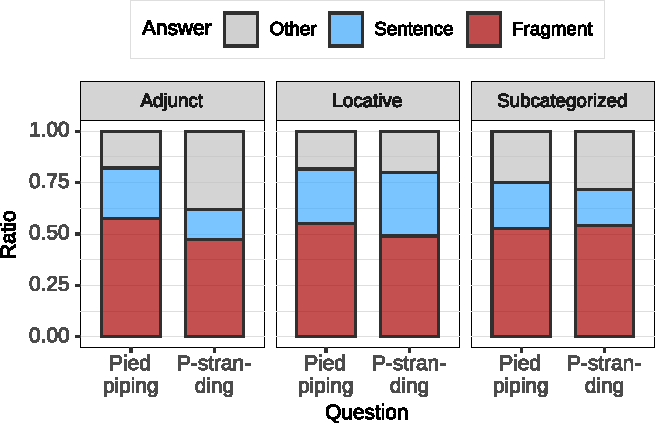
\includegraphics[scale=1]{figures/ex8_prod_answers}
 \caption{Ratios of answer categories in exp. 4. ``Other'' indicates indirect answers or constructions not involving P-stranding/Pied-piping\label{fig:ex8_prod_relfrag}.}
\end{figure}

Figure \ref{fig:ex8_prod_fragments} gives an overview of the direct fragment answers by condition and answer type. Across all conditions the preposition was omitted\is{Preposition omission} more often in the answer (82.4\%) than it was realized, both when the answer preposition was stranded\is{Preposition stranding} (84.1\%) in the question and when it was pied-piped\is{Pied-piping} (80.8\%). In order to test whether the form of the \textsc{Question} and the \textsc{PPType} (locative / adjunct\is{Adjunct} / subcategorized) had an effect on the likelihood of preposition omission\is{Preposition omission} in the answer, the data were analyzed with logistic mixed effects regressions fitted with the \texttt{lme4} \citep{bates.etal2015} package in \texttt{R} following the procedure described in Section \ref{sec:intro-stats}. The regressions predicted the likelihood of the \textsc{Omission} of the preposition in the answer. Ten subjects who produced less than five direct fragment answers were excluded from the analysis, this resulted in the loss of a further 3.3\% of the remaining data.

\begin{figure}
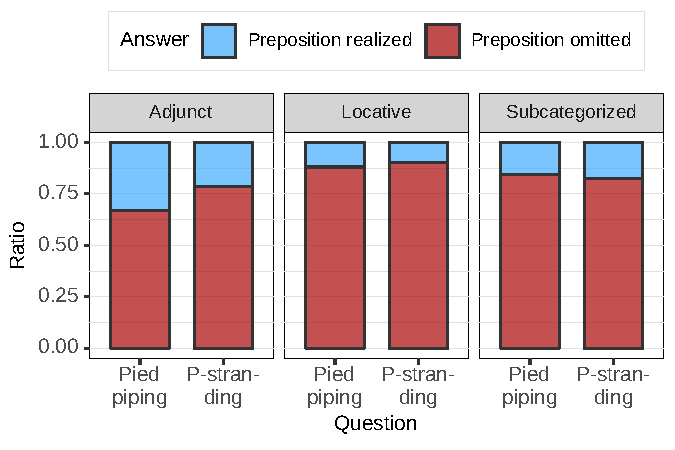
\includegraphics[scale=1]{figures/ex8_prod_relfrag_answers}
 \caption{Ratio of preposition omission/realization across conditions\label{fig:ex8_prod_fragments}.}
\end{figure}

\textsc{PPType} was a ternary factor, therefore the data had to be analyzed by conducting pairwise comparisons between factor levels just like in experiment \ref{exp:pstranding-defaultcase}. A first analysis compared the two types of complement PPs\is{Preposition phrase}, i.e. locative and subcategorized PPs, which each other. The initial model contained main effects for \textsc{Question}, \textsc{PPType}, \textsc{Position} (numeric) and all two-way interactions between these predictors. The model had only random intercepts for subjects and items, because it did converge with a more complex random effects structure. As the difference between locative and subcategorized PPs\is{Preposition phrase} did not turn out to be significant \glmernonsig{0.57}{0.5}, these conditions were pooled for further analysis and hence compared only adjunct\is{Adjunct} to complement PPs\is{Preposition phrase}. 

After pooling locative and subcategorized PPs\is{Preposition phrase}, the complete data set could be analyzed at once. 
The initial model contained main effects for \textsc{Question}, \textsc{PPType} (now binary), \textsc{Position} and all two-way interactions between these predictors. The model had only random intercepts for subjects and items and a by-subject random slope for \textsc{PPType}, because it did not converge with a more complex random effects structure. The final model (see Table \ref{tab:pstranding-production-estimates}) contains significant effects for both IVs: The preposition in the short answer fragment\is{Fragment, short answer} is more likely to be omitted\is{Preposition omission} when the PP\is{Preposition phrase} is a complement than when it is an adjunct\is{Adjunct} \glmer{5.23}{0.05}. What is more important with respect to the goal of the experiment is that the preposition is also more likely to be omitted\is{Preposition omission} in the answer when it is stranded\is{Preposition stranding} in the question \glmer{4.85}{0.05}. There is no significant interaction between the IVs  \glmernonsig{0.86}{0.3}.

\begin{table}
\begin{tabular}{l c c c c c}
\lsptoprule
Predictor & Estimate & SE & $\chi^2$ &  $p$ &  \\   
\midrule
\textsc{Question} & 0.719 &  0.308 & 4.85 & \textless 0.05 & * \\
\textsc{PPType} & 1.822 &     0.727 &   5.23 &  \textless 0.05 & *\\
\lspbottomrule
\end{tabular}
\caption{Fixed effects in the final GLMM for experiment \ref{exp:pstranding-production}.\label{tab:pstranding-production-estimates}}
\end{table}

\subsubsection{Discussion}
Experiment \ref{exp:pstranding-production} had the purpose of testing the nonsyntactic explanation for the crosslinguistic coincidence between the availability of preposition omission\is{Preposition omission} in short answers\is{Fragment, short answer} and of P-stranding\is{Preposition stranding} in questions: Speakers tend to match the form of the answer with that of the question, therefore, if a language has no P-strand\-ing\is{Preposition stranding} in questions, preposition omission\is{Preposition omission} in the answer will be degraded. The experiment supports this hypothesis: If the preposition is stranded\is{Preposition stranding} in the question it is significantly more likely to be omitted\is{Preposition omission} than when it is pied-piped\is{Pied-piping}. This is the result that question-answer parallelism predicts.

In absolute terms, the effect seems to be less pronounced than the one found by \citet{nykiel2017} in her corpus study\is{Corpus}. This could be in part due to the restriction to P-stranding\is{Preposition stranding} and pied-piping\is{Pied-piping} questions as antecedents, whereas \citet{nykiel2017} investigated a larger variety of antecedents and remnants. Furthermore, the experimental design might have contributed to reducing the effect of the antecedent. First, although they were not told to do so, a few participants noted that some of the questions were not totally natural by adding a comment like ``the question sounds odd'' in the text field.%
%
\footnote{These responses were not analyzed.}\afterfn%
%
As I discussed above, P-stranding\is{Preposition stranding} is preferred in colloquial speech (recall that the experimental stimuli were presented as informal dialogues) for complement PPs\is{Preposition phrase} and dispreferred for adjunct\is{Adjunct} PPs\is{Preposition phrase}. Therefore, in each condition one of the questions is not perfectly natural, and in natural settings there is probably a higher ratio of P-stranding\is{Preposition stranding} in questions for complement than for adjunct\is{Adjunct} PPs\is{Preposition phrase}. Since the form of the question affects that of the answer, in corpus\is{Corpus} data this would probably increase the difference in counts of each of the answer variants as compared to the more controlled setting of the experiment. Second, even though the \textsc{Position} effect is not significant, subjects produced a relatively large amount of answers throughout the experiment and probably got used to the task and matched their answers to a lesser degree to the form of the question due to familiarization. This is tentatively supported by the observation that parallelism is most pronounced for the first item that each subject saw: Subjects who saw a complement PP in the question almost always omitted the preposition\is{Preposition omission} in the answer (90\% omission rate for pied-piping\is{Pied-piping} and 90.9\% for P-stranding\is{Preposition stranding}), but only 16.7\% of those who saw a pied-piped\is{Pied-piping} adjunct\is{Adjunct} PP in the question and all of those who saw a P-stranded\is{Preposition stranding} one did so. These numbers are not significant due to the reduced number of observations, but they suggest that a crowdsourced experiment with only one trial per subject might be a promising option to prevent such a familiarization effect.

The preference for preposition omission\is{Preposition omission} in all conditions is in line with the English\il{English} corpus\is{Corpus} data in \citet{nykiel2017}. She also reports that the preposition is omitted\is{Preposition omission} more often than it is realized both when it is pied-piped\is{Pied-piping} and stranded\is{Preposition stranding} in the antecedent. This overall preference for preposition omission\is{Preposition omission} is unexpected under the structured propositions account of question-answer parallelism. If pied-piping\is{Pied-piping} occurs because the preposition belongs to the focus of the question, and the focus structure of the answer is determined by that of the question, one would theoretically expect a perfect match between both. Such an effect can be reduced in experimental settings, but pied-piping\is{Pied-piping} in the question does not result in an inversion of participants' preferences in any of the conditions. The data are therefore tentatively more in line with the structural persistence account. From a processing\is{Processing effort} perspective, competing constraints introduce a probabilistic bias that can be overridden by others. Speakers might tend to omit the preposition\is{Preposition omission} because it is given, and this constraint might cancel out part of the effect of the tendency to reuse material given in context. Furthermore, the effect of constraints that are specifically relevant for oral on-line communication might be less prominent in experimental settings.%
%
\footnote{See e.g. \citet{zhan.etal2017}, who did not find effects of audience design\is{Audience design} in a production study\is{Production task}, even though such effects had been attested in related previous work.}\afterfn
%
Recall also that the relative acceptability of proper noun DP\is{Determiner phrase} fragments as short answers\is{Fragment, short answer} to PP\is{Preposition phrase} questions \citep{lemkeaccepted} also suggests that some deviation from question-answer congruence is possible even in German\il{German}. This is unexpected under a semantic account.

The main effect of \textsc{PPType} is in line with the observation by \citet{vanriemsdijk1978} that P-stranding\is{Preposition stranding} is less acceptable in adjunct\is{Adjunct} than in complement PPs\is{Preposition phrase}. However, this tendency does not override the preference for omitting the preposition\is{Preposition omission} in the experiment: The ratio of omitted prepositions\is{Preposition omission} is indeed the lowest observed throughout the experiment if the PP is an adjunct\is{Adjunct} and the preposition pied-piped\is{Pied-piping} in the question (see Figure \ref{fig:ex8_prod_fragments}). Still, even in this case, 67\% of prepositions are omitted\is{Preposition omission}. This might suggest that the syntactic relationship between the preposition and the verb at least affects preposition omission\is{Preposition omission} in fragments.

Taken together, the production study\is{Production task} supports a nonsyntactic question-an\-swer parallelism. If the form of short answers\is{Fragment, short answer} follows that of questions, the absence of P-stranding\is{Preposition stranding} in German\il{German} questions explains straightforwardly why DP\is{Determiner phrase} fragments are degraded in such contexts. The experiment does not allow for a conclusion on why we observe this parallelism, but the strong overall preference for omitting the preposition\is{Preposition omission} in the answer seems to be more in line with a processing\is{Processing effort} account than with the structured propositions approach. This finding does not falsify the movement and deletion\is{Movement and deletion account} account. Movement and deletion\is{Movement and deletion account} is neither incompatible with the assumption of differing focus structures between pied-piping\is{Pied-piping} and P-stranding\is{Preposition stranding} questions nor with structural persistence. However, both of these accounts explain the pattern observed for fragments without assuming movement as an obligatory step\is{Movement and deletion account} in the derivation of fragments. This clearly weakens the status of the PSG\is{P-Stranding Generalization} as genuine evidence for movement.

\subsection{General discussion: Preposition omission} \label{sec:pstranding-discussion}
In section \ref{sec:pstranding} I presented four experiments that tested the predictions of the PSG\is{P-Stranding Generalization}, which is taken to be one of the central pieces of evidence for movement\is{Movement and deletion account} in fragments, and the viability of non-movement explanations for the data. Experiments \ref{exp:pstranding-german} and \ref{exp:pstranding-english} empirically support the predictions of the PSG\is{P-Stranding Generalization} for German\il{German}, where prepositions are obligatorily pied-piped\is{Pied-piping} in questions, and for English\il{English}, which allows for P-stranding\is{Preposition stranding}. Just like the PSG\is{P-Stranding Generalization} predicts, in German\il{German} there is a strong preference for realizing the preposition, whereas in English\il{English} its omission\is{Preposition omission} is acceptable, and actually preferred in the context of questions with P-stranding\is{Preposition stranding}.

A further result of experiment \ref{exp:pstranding-english} is that fronting the PP\is{Preposition phrase} in a complete sentence in English\il{English} is heavily degraded, as has been already noted by \citet{weir2014a}. This questions some of the arguments by \citet{merchant2004}, which are based on the idea that the acceptability of fragments patterns with that of left dislocation structures. The low ratings for both pied-piping\is{Pied-piping} and P-stranding\is{Preposition stranding} in the answer suggest that a movement and deletion\is{Movement and deletion account} account is viable only if exceptional movement\is{Exceptional movement account} is assumed, as \citet{weir2014} proposes. The exceptional movement\is{Exceptional movement account} account however requires an explanation for why the preposition is sometimes pied-piped\is{Pied-piping} in English\il{English}. If extraction out of the PP\is{Preposition phrase} is possible, and only the DP\is{Determiner phrase} complement of P is focused, there is no need to front the complete PP\is{Preposition phrase} in English\il{English}. For German\il{German} this is not a problem, because pied-piping\is{Pied-piping} is the only way to extract the focused DP\is{Determiner phrase} out of the ellipsis site if extraction out of PP\is{Preposition phrase} is blocked for independent reasons in this language.

Although the experiments \ref{exp:pstranding-german} and \ref{exp:pstranding-english} are in line with the PSG\is{P-Stranding Generalization}, they only provide evidence for movement\is{Movement and deletion account} if explanations under derivationally simpler accounts, such as the nonsentential\is{Nonsentential account} and in situ deletion\is{In situ deletion account} accounts, must be ruled out. Experiments \ref{exp:pstranding-defaultcase} and \ref{exp:pstranding-production} tested two of these alternative explanations.

Experiment \ref{exp:pstranding-defaultcase} investigated the hypothesis that, as suggested by \citet{barton.progovac2005}, the preposition cannot be omitted\is{Preposition omission} in languages with strong case features\is{Case feature} because prepositional case\is{Prepositional case} is structural case\is{Structural case} and must always be checked. According to their theory, prepositional case\is{Prepositional case} cannot be checked in fragments because there is no unarticulated syntactic material that could do so (in this case, a preposition). Instead, they expect DPs\is{Determiner phrase} to appear in default case. The data clearly disconfirm this prediction: Default case\is{Default case} was rated\is{Acceptability rating task} even worse than the significantly degraded prepositional case\is{Prepositional case}-marked DPs\is{Determiner phrase}. Consequently, the case checking\is{Case feature} hypothesis, at least in the version suggested by \citet{barton.progovac2005}, must be discarded. Experiment \ref{exp:pstranding-defaultcase} also provides further evidence against the nonsentential account\is{Nonsentential account}, because presumably ungrammatical prepositional case\is{Prepositional case}-marked DP fragments are rated\is{Acceptability rating task} as more acceptable than grammatical, yet possibly pragmatically odd, nominative\is{Nominative case} DP fragments. Furthermore, the experiment questions the cleft\is{Cleft}-based analysis of preposition-less fragments in languages that lack P-stranding\is{Preposition stranding} \citep{szczegielniak2008, rodrigues.etal2009}. In German\il{German}, fragments derived from clefts\is{Cleft} must exhibit nominative\is{Nominative case} case morphology, but the experiment shows that nominative\is{Nominative case} DP fragments are degraded not only as compared to PPs\is{Preposition phrase} but also to presumably ungrammatical prepositional case\is{Prepositional case}-marked DP fragments.

Experiment \ref{exp:pstranding-production} addressed the hypothesis that the crosslinguistic variation found in fragments is the result of a tendency for answers to structurally match the corresponding questions. I discussed two possible explanations for this, one in terms of a structured propositions account of question semantics \citep{reich2002, griffiths2019} and one based on a tendency to reuse syntactic structure from previous discourse \citep{levelt.kelter1982}. Question-answer parallelism provides a straightforward account of the P-Stranding Generalization\is{P-Stranding Generalization}: If the preposition is pied-piped\is{Pied-piping} in the question, it is necessarily, or at least preferably, realized in the answer. Since the preposition is always pied-piped\is{Pied-piping} in languages like German\il{German}, it is never omitted\is{Preposition omission} in short answers\is{Fragment, short answer}. For languages that allow for both pied-piping\is{Pied-piping} and P-stranding\is{Preposition stranding}, the form of an answer would tend to match that of the question: Pied-piping\is{Pied-piping} in the question would yield a relatively higher ratio of PP\is{Preposition phrase} short answers\is{Fragment, short answer}, and P-stranding\is{Preposition stranding} more DP\is{Determiner phrase} short answers\is{Fragment, short answer}. Experiment \ref{exp:pstranding-production} provides evidence for such a preference using a production task\is{Production task}. The experiment could hence replicate the effect observed in a corpus study\is{Corpus} by \citet{nykiel2017} and the evidence for structural parallelism by \citet{levelt.kelter1982} in a controlled experiment that investigated specifically effects of P-stranding\is{Preposition stranding}/pied-piping\is{Pied-piping} in question on the form of the answer. However, despite a significant effect of the question's form, preposition omission\is{Preposition omission} was preferred in all conditions in absolute terms. The parallelism between question and answer seems to be weaker than expected under a structured propositions account, hence an explanation in terms of structural persistence tentatively seems to fit the observed pattern better.

The evidence for question-answer parallelism does not contradict the movement and deletion\is{Movement and deletion account} account, because syntactic theories do not neglect effects of processing\is{Processing effort} constraints but restrict the set of alternative expressions on which such constraints operate. However, experiment \ref{exp:pstranding-production} evidences that the form of the question affects the form of the answer in English\il{English}. If it does so in German\il{German} too, this provides a straightforward non-movement explanation for the preposition omission\is{Preposition omission} data: DP\is{Determiner phrase} short answers\is{Fragment, short answer} are not degraded in German\il{German} because they are ungrammatical, but because they never match the form of the question. As I argued above, it depends on the viability of non-movement accounts of the preposition omission\is{Preposition omission} data whether they constitute evidence for movement or not. The parallelism between question and answer evidenced in my experiment and in \citet{nykiel2017} provides such an explanation and consequently undermines the status of the preposition omission\is{Preposition omission} data as evidence for movement\is{Movement and deletion account}.

Taken together, preposition stranding\is{Preposition stranding} does not uniquely support the movement and deletion\is{Movement and deletion account} account as strongly as claimed by \citet{merchant2004}. Specifically, the data can be equally well explained in terms of question-answer parallelism under the assumption of and in situ deletion\is{In situ deletion account} account. The nonsentential account\is{Nonsentential account} is of course also compatible with processing constraints\is{Processing effort}, however it predicts that prepositions cannot be omitted\is{Preposition omission} if the DP\is{Determiner phrase} is case-marked. This has been disconfirmed by experiment \ref{exp:pstranding-defaultcase}. In the next section I investigate a further movement restriction\is{Movement restriction} on complement clause\is{Complement clause} topicalization, which has been argued to hold crosslinguistically in Germanic languages \citep{webelhuth1992} and that has already been empirically investigated by \citet{merchant.etal2013}.


\section{Movement restrictions: Complementizer omission}\label{sec:ccs}
\largerpage

\subsection{Complementizer omission as evidence for movement}\label{sec:ccs-background}
\subsubsection{Movement restrictions on complement clauses}
\begin{sloppypar}
The second movement restriction\is{Movement restriction} that I investigate empirically is the (im)possibi\-lity of fronting complementizer-less\is{Complementizer omission} complement clauses\is{Complement clause} (in what follows, CCs\is{Complement clause}).%
%
\footnote{\citet[83--85]{webelhuth1992} argues that a similar pattern holds across all Germanic languages, the difference being that some do not allow for complementizer omission\is{Complementizer omission} in situ.} %
%
This restriction is particularly relevant to the movement and deletion\is{Movement and deletion account} account because \citet{merchant2004} argues that it constrains the form of fragments and \citet{merchant.etal2013} present empirical evidence in support of this prediction.\end{sloppypar}

According to \citet{merchant2004}, it was \citet{stowell1981} who first noted that only CCs\is{Complement clause} headed by an overt complementizer can appear in a sentence-initial position.%
%
\footnote{\citet{stowell1981} in turn attributes the observation to \citet{kayne1981}, but \citet[744]{morgan1973} makes a similar point even before that.}\afterfn%
%
\citet[396f]{stowell1981} observes that this holds for both subject CCs\is{Complement clause} \Next[a] and topicalized object CCs\is{Complement clause} \Next[b]. \Next[c] shows that omitting the complementizer\is{Complementizer omission} in object position is possible, hence the ungrammaticality must be attributed to the sentence-initial position of the CC.%
%
\footnote{
\citet[396]{stowell1981} explains the data by arguing that complementizer-less CCs\is{Complement clause} are headed by a phonetically null element, which c-commanded by the verb according to the Empty Category Principle \citep{chomsky1981}. This is possible only in the complement position, but not when the clause is base-generated in the subject position \Last[a] or moved to the topic position \Last[b].}\afterfn%
%

\ex. \a. *(That) the teacher was lying was hardly obvious.
      \b. *(That) the teacher was lying, Ben already knew.
 \c. Ben knew the teacher was lying.

\citet{merchant2004} cites \citet{morgan1973} with the observation that the same restriction holds for CP\is{Complementizer phrase} fragments, under the condition that the speaker ``does not believe or subscribe to [the meaning of the fragment, R.L.]'' \citep[690]{merchant2004}, i.e. when it is non-factive\is{Factivity} \Next[a]. The contrast between \Next[b] and \Next[c] shows that the complementizer is obligatory only when the CC\is{Complement clause} is topicalized \Next[c], but that it can be omitted\is{Complementizer omission} when the CC\is{Complement clause} remains in situ. 

\ex.
\a. What does no one believe? \hfill \citep[690]{merchant2004}\\
\mbox{}\hspace{-.45em}\#(That) I’m taller than I really am.
\b. No one believes (that) I'm taller than I really am. \label{ex:merchant-cc-insitu}
\c. *(That) I’m taller than I really am, no one believes. \label{ex:merchant-cc-fronted}

\begin{sloppypar}\noindent
\citeauthor{merchant2004} argues that this challenges in situ deletion accounts\is{In situ deletion account} of fragments, which must explain why the complementizer cannot be omitted\is{Complementizer omission} in fragments even though this is possible in full sentences when the CC\is{Complement clause} appears in situ.\end{sloppypar}

Taken together, according to the literature the pattern seems to be robust for non-factive\is{Factivity} CCs\is{Complement clause} of verbs: Only CCs\is{Complement clause} with overt complementizers may be fronted. If the derivation of fragments involves regular A'-movement, as \citet{merchant2004} claims, this predicts fragment CCs\is{Complement clause} to always require overt complementizers. As I repeatedly noted above, if exceptional movement\is{Exceptional movement account} is assumed, it is crucial to determine whether this movement is available ``in principle'' or not, but \citet{weir2014} does not provide criteria that determine whether this is true for a specific movement operation. Since the literature on the phenomenon cites no acceptable instance of this beyond parenthetical uses,%
\footnote{\citet{webelhuth1992} argues that the following example is fine, provided an intonational break after the first clause:

\exg. [Hans ist krank gewesen] hat Peter gemeint.\\
Hans is sick been has Peter meant\\
\trans{Peter thought Hans had been sick.} \exsourceraised{\citep[89]{webelhuth1992}}

}\afterfn%
%
it is probably to be classified as not available in principle. Non-movement accounts in turn require an independent explanation for why the complementizer cannot be omitted\is{Complementizer omission}. However, the pattern is currently only partially empirically supported. Therefore, before any conclusions can be drawn it must be empirically investigated whether it actually holds. This is the goal of the experiments in Section \ref{sec:ccs}. 

\subsubsection{Previous experimental evidence}
\citet{merchant.etal2013} present first experimental evidence for an apparent parallelism between the movement restriction\is{Movement restriction} on complementizer-less\is{Complementizer omission} CCs\is{Complement clause} and the form of fragments. In their experiment 1, they tested short answer fragments\is{Fragment, short answer} like \Last[a] in an acceptability rating\is{Acceptability rating task} study. They find that fragments headed by an overt complementizer ($\mu$ = 4.25 on a 5-point scale, where 5 = perfect) are rated\is{Acceptability rating task} significantly better than complemen\-tizer-less ones ($\mu$  = 3.73) and interpret this as reflecting a movement restriction\is{Movement restriction} on comple\-mentizer-less CCs\is{Complement clause}. Since movement and deletion\is{Movement and deletion account} predicts that complementizer omission\is{Complementizer omission} is ungrammatical, the ratings for these fragments are surprisingly high. \citet{merchant.etal2013} suggest that this is due to the possibility of interpreting complementizer-less\is{Complementizer omission} CCs\is{Complement clause} as indirect answers. With an indirect answer, the speaker does not give a congruent answer to the question (as discussed in Section \ref{sec:theories-insitu}), but provides any piece of information that might help his interlocutor to figure out an answer. For instance, in \Next Mary does not commit herself to the claim that the defeat is the reason for John being angry, but she suspects that the defeat might be the reason for John's anger.

\ex. Bill: Why is John so angry?\\
    Mary: (I'm not sure, but) Barcelona lost to Liverpool yesterday.
    
The study by \citet{merchant.etal2013} leaves open several issues: (i) Acceptability ratings\is{Acceptability rating task} were collected only for fragments,  (ii) some items include CCs\is{Complement clause} of prepositions, (iii) some of the matrix verbs are factive\is{Factivity}, and (iv) they do not explore alternative explanations that do not imply movement for the data. In what follows I review these issues in greater detail.\largerpage

First, \citet{merchant.etal2013} tested the acceptability\is{Acceptability rating task} of fragment CCs\is{Complement clause} but not of corresponding topicalization structures. The authors assume that the introspective contrast between \ref{ex:merchant-cc-insitu} and \ref{ex:merchant-cc-fronted}, which has been repeatedly cited in the literature since \citet{stowell1981}, accounts for the measured acceptability of the corresponding fragments. However, some native speakers of American English\il{English} that I consulted do not share the grammaticality judgments that \citet{merchant.etal2013} assign to the topicalized CCs\is{Complement clause}. Furthermore, \citet{featherston2007} notes that introspective data sometimes do not generalize to a larger population and withstand empirical investigation despite of being widely agreed on and repeatedly cited in the theoretical literature. The validity of the pattern in \LLast however is crucial to the experiment by \citet{merchant.etal2013}: If it was not confirmed, the judgments for fragments could not be attributed to those for the presumably underlying left dislocation structures. This calls for an empirical investigation of both the fragments and corresponding left dislocation structures.

Second, half ($n = 8$) of the items tested by \citet{merchant.etal2013} involve CCs\is{Complement clause} which are embedded under a PP\is{Preposition phrase}, like \Next. These CCs\is{Complement clause} are always ungrammatical in situ \Next[a], whereas they are acceptable when the complementizer is present in a fronted position \Next[b] and as a fragment \Next[c]. Even though \citet{merchant2004} argues that this speaks against the in situ deletion\is{In situ deletion account} account, actually it does not: In situ deletion\is{In situ deletion account} takes regular grammatical sentences as the input for ellipsis and analyzes ellipsis as a post-spellout phenomenon. If movement of the CC\is{Complement clause} is obligatory for whatever reason, it has to occur before ellipsis, so that the only grammatical input for in situ deletion\is{In situ deletion account} is \Next[b] with an overt complementizer.

\ex. What are you ashamed of?
\a. *I am ashamed of (that) I ignored you.
\b. *(That) I ignored you, I am ashamed of.
\c. *(That) I ignored you.

\is{Factivity|(}Third, among the remaining eight items, some contained factive\is{Factivity} matrix verbs, like \textit{to regret} in \Next. Factive\is{Factivity} verbs, which presuppose the truth of their complement, as \textit{to regret} or \textit{to conceal} do, are widely assumed to require, or at least strongly prefer, CCs\is{Complement clause} with overt complementizers (see \citenob{kiparsky.kiparsky1970}; \citenob{hegarty1992}). \citet[689]{merchant2004} himself cites a related observation by \citet{morgan1973} that complementizers may not be omitted\is{Complementizer omission} when the speaker ``does not believe or subscribe'' to the content of the CC. Consequently, if the verb disprefers or even disallows complementizer-less\is{Complementizer omission} CCs\is{Complement clause} in general, any structure derived from it will be degraded, independently of whether the CC\is{Complement clause} is moved to the left periphery or whether the matrix clause is PF-deleted in situ.\is{Factivity|)}

\ex. What did John regret? \hfill \citep[31]{merchant.etal2013}\\
(That) he joined the Navy.

Finally, there are potential non-movement explanations for both the empirically observed fragment data and the introspective judgments on topicalization. As for fragments, a complementizer-less\is{Complementizer omission} answer can be interpreted both as a direct and as an indirect answer to a question, whereas a complementizer unambiguously marks the answer as direct. 
Therefore, the ratings reported by \citet{merchant.etal2013} possibly do not reflect grammaticality, but usage preferences. 
In what refers to complementizer omission\is{Complementizer omission} in full sentences, realizing the complementizer in fronted clauses could facilitate processing. When the hearer parses\is{Parser, human} a complementizer-less\is{Complementizer omission} CC, the complement clause\is{Complement clause} can be incorrectly analyzed as a matrix clause until the matrix verb is encountered. In contrast, the initial complementizer requires that the CC\is{Complement clause} is parsed\is{Parser, human} as the complement of a verb, and this will facilitate processing. This is also in line with corpus\is{Corpus} data by \cite{jaeger2010}, who shows that the likelihood of a CC\is{Complement clause} in a specific context predicts whether the complementizer will be omitted\is{Complementizer omission} or not.%
%
\footnote{The possibility of a processing account has already been discussed by \citet[397]{stowell1981}, who argues against the processing account based on data as \Next. The argument is that the CC\is{Complement clause} is very likely at the point where it occurs due to the subcategorization preferences of the predicate, and still the complementizer cannot be omitted\is{Complementizer omission}.

\ex. It surprises me *(that) you have heard about Roger.  \hfill \citet[397]{stowell1981}

}\afterfn%
%

In Section \ref{sec:ccs} I present experiments based on the study on complement clauses\is{Complement clause} by \citet{merchant.etal2013} in German\il{German} and English\il{English} (experiments \ref{exp:ccs-german} and \ref{exp:ccs-english}), which address these issues. In the I collect ratings for both topicalized and fragment CCs\is{Complement clause}, test only CCs\is{Complement clause} that are acceptable in situ and use only non-factive\is{Factivity} matrix verbs. The goal of the experiments is two-fold. First, the data for fragment answers will show whether the preference for realizing the complementizer in fragments is replicated when controlling for factivity\is{Factivity}. Second, the data for left dislocation answers might provide empirical evidence for the movement restriction\is{Movement restriction} on complementizer-less\is{Complementizer omission} CCs\is{Complement clause} on which the experiment by \citet{merchant.etal2013} is based. Anticipating the results, the experiments suggest that the effect reported by \citet{merchant.etal2013} does not evidences a movement restriction\is{Movement restriction} on complementizer-less\is{Complementizer omission} CCs\is{Complement clause} but results from independent factors. The German\il{German} data replicate the preference for realizing the complementizer in fragments, but this effect is not reflected in the acceptability of the corresponding left dislocation structures. In English\il{English}, there is no significant difference between fragments at all and null complementizers are even preferred in full sentences.

\refstepcounter{expcounter}\label{exp:ccs-german}
\subsection{Experiment \ref{exp:ccs-german}: CC topicalization in German}\label{sec:ccs-german}
\largerpage[1.75]

\subsubsection{Background}\label{sec:ccs-german-background}
Experiment \ref{exp:ccs-german} replicates experiment 1 in \citet{merchant.etal2013} in German\il{German} under more controlled conditions. As compared to the study by \citet{merchant.etal2013}, there were four main modifications: First, the experiment was conducted in German, second, I used a context story to preclude the possibility of an indirect answers interpretation, third, I tested both fragments and full sentences, and fourth, I added a third condition, subjunctive mood verb-second CCs\is{Complement clause}.

As for the first modification, in German I expected a similar pattern to the English data in \citet{merchant.etal2013}. \citet[83]{webelhuth1992} claims that subject CCs\is{Complement clause} require overt complementizers in all Germanic languages.%
%
\footnote{\citeauthor{webelhuth1992} presents \Next as evidence in favor of this claim. However, omitting the complementizer\is{Complementizer omission} in verb-last CCs\is{Complement clause} is also unacceptable in situ and cannot be attributed to the prefield\is{Prefield} position \NNext[a]. In the case of the example, its verb-second counterpart \NNext[b] seems to be degraded as well. A further shortcoming of the example is that the predicate is factive\is{Factivity}, so that complementizer omission\is{Complementizer omission} seems to be dispreferred in situ \NNext[c]. \NNext[c] is only acceptable with a break in intonation between the first and the second clause that marks that each clause is an independent sentence.

\exg. *(Da\ss) Hans nicht kommt, ist schade.\\
that Hans not comes is pity\\
\trans{It is a pity that Hans does not come.}\exsourceraised{\citep[83]{webelhuth1992}}

\ex. \ag. Es ist schade, *(dass) Hans nicht kommt.\\
	  it is pity that Hans not comes\\
     \bg. *Hans kommt nicht, ist schade.\\
	  Hans comes not is pity\\
    \cg.  *Es ist schade, Hans kommt nicht.\\
	  it is  pity Hans comes not\\
	  \trans{It is a pity (that) Hans does not come.}


}\afterfn %

The target sentence was introduced by a context story and a short dialogue with two turns per speaker \Next. The context story had the purpose of making an indirect answer less likely. \citet{merchant.etal2013} suggest that complementizer-less\is{Complementizer omission} CCs\is{Complement clause} were rated\is{Acceptability rating task} as relatively acceptable\is{Acceptability rating task} in their experiment due to their interpretation as indirect answers. In my experiment, the context stories ensured that this was not possible: For instance, in \Next, it is very unlikely that the reporter has sufficient knowledge about the crime to give an indirect answer. The CCs\is{Complement clause} were tested not only as fragments, but also in a left-peripheral position within a complete sentence in order to investigate whether the assumed movement restriction\is{Movement restriction} on complementizer-less\is{Complementizer omission} CCs\is{Complement clause} is empirically confirmed. Furthermore, acceptability differences between the sentential conditions allow me to test the prediction of the movement and deletion\is{Movement and deletion account} account that the acceptability of left dislocations matches that of the corresponding fragments.

Finally, besides the German\il{German} counterparts of the CCs\is{Complement clause} investigated by \citet{merchant.etal2013}, I added a third type of complement clause\is{Complement clause}, verb-second complement clause\is{Complement clause}s in subjunctive mood, to test the hypothesis that verb-second CCs\is{Complement clause} are rated\is{Acceptability rating task} as acceptable because they are interpreted as indirect answers.

\ex. [Context story] This weekend a famous painting has been stolen from the museum. The newscaster is reporting on the investigation of the robbery.\\ \mbox{}[Newscaster:] What's the news about the art robbery?\\ \mbox{}[Reporter:] The investigators are discussing how the burglar got into the building.\label{ex:ccs-experiment-sample-item}
\ag. [N:] Was glaubt Kommissar Wagner?\\
\mbox{} what believes inspector Wagner\\
\trans{[N:] What does inspector Wagner believe?}
\bg. [R:] Dass der Täter durch  das Fenster  eingestiegen ist.\\
     \mbox{} that  the thief through the window  entered is\\
     \trans{[R:] That the thief entered through the window.}

The reason for this is that CCs\is{Complement clause} headed by \textit{dass}, the German\il{German} equivalent to \textit{that}, are verb-last, whereas complementizer-less\is{Complementizer omission} CCs\is{Complement clause} are always verb-second. Therefore, verb-second complement clause\is{Complement clause}s are ambiguous between a direct answer (a CC\is{Complement clause} fragment) and an indirect answer (a matrix clause). Since subjunctive mood encodes reported speech in German\il{German}, it enforces the interpretation as a direct answer. If indicative complementizer-less\is{Complementizer omission} CCs\is{Complement clause} were rated\is{Acceptability rating task} as more acceptable only because they can be interpreted as indirect answers, they would be more acceptable than subjunctive ones. Subjunctive might also provide some insights on the viability of the pragmatic and processing accounts of complementizer omission\is{Complementizer omission} that I sketched above. If complementizer-less\is{Complementizer omission} fragments are dispreferred due to their ambiguity\is{Ambiguity}, subjunctive should improve their acceptability because it excludes the possibility of an indirect answer. Similarly, in fronted CCs\is{Complement clause} the likelihood of an embedding matrix verb will increase as soon as the inflected verb in the CC\is{Complement clause} is encountered. Since the CC\is{Complement clause} is verb-second, this happens relatively early, hence processing\is{Processing effort} it should be easier in comparison to the indicative verb second clause. This setting yields a 2$\times$3 design that crosses \textsc{Sententiality} and \textsc{CCType}.

The movement and deletion\is{Movement and deletion account} account predicts that, if complementizer-less\is{Complementizer omission} CCs\is{Complement clause} are degraded as full sentences, they will be as fragments, too. If the movement restriction\is{Movement restriction} on complementizer-less\is{Complementizer omission} CCs\is{Complement clause} was not empirically supported, \citet{merchant2004} predicts that whatever pattern is observed, there should be no interaction between \textsc{Sententiality} and \textsc{CCType}. The in situ deletion\is{In situ deletion account} account makes no specific predictions with respect to this, because it does not assume that left dislocation structures are the input to the derivation of fragments. In situ deletion\is{In situ deletion account} might predict a parallelism between the acceptability of complement clauses\is{Complement clause} as fragments and in their base position, but if both the realization and the omission of the complementizer is grammatical for non-factive\is{Factivity} matrix verbs it is unlikely that this results in a strong acceptability contrast.

\subsubsection{Materials}\label{sec:ccs-materials}
All materials follow the pattern in \Last. The target utterance is preceded by a two-sentence context story and a dialogue between two characters. The context story is always such that the character who produces the target utterance is not in the epistemic position to produce an indirect answer. The target utterance is the second turn by the second character. In the sentential conditions, the matrix clause in the target utterance (\textit{glaubt er}, `he believes') is given in the immediately preceding question. Table \ref{tab:ccs-german-materials} provides an overview of the conditions for the target sentence in \Last.

The issue that factive verbs\is{Factivity} prefer CCs\is{Complement clause} with overt complementizers according to the literature \citep{kiparsky.kiparsky1970, hegarty1992} was addressed by testing only three non-factive\is{Factivity} matrix verbs (\textit{glauben} `to believe’, \textit{meinen} `to mean' and \textit{sagen} `to say'). A corpus\is{Corpus} search on the German\il{German} newspaper corpus\is{Corpus} TüBa-D/Z \citep{telljohann.etal2004} confirms that each of the three verbs occurs with each of the CC\is{Complement clause} types investigated, but they seem to differ quantitatively in their subcategorization preferences, as Table \ref{tab:ccs-matrixv-frequency} shows. In order to factor out possible subcategorization preferences of specific verbs I included the \textsc{MatrixVerb} as a predictor in the statistical analysis. However, the analysis showed that the verb has no significant effect on acceptability.

\begin{table}
 \begin{tabular}{l l l}
 \lsptoprule
  Target utterance & Condition\\
\midrule
Dass der Täter durch  das Fenster  eingestiegen ist, glaubt er. &VL, sent.\\
Der Täter ist durch das Fenster  eingestiegen, glaubt er. & V2, ind, sent.\\
Der Täter sei durch das Fenster  eingestiegen, glaubt er. & V2, ind, sent.\\
Dass der Täter durch  das Fenster  eingestiegen ist. &VL, frag.\\
Der Täter ist durch das Fenster  eingestiegen. & V2, ind, frag.\\
Der Täter sei durch das Fenster  eingestiegen. & V2, ind, frag.\\

  \lspbottomrule
 \end{tabular}
\caption{Target sentences in experiment \ref{exp:ccs-german}. See example \ref{ex:ccs-experiment-sample-item} for glosses. The subjunctive  is distinguished from indicative only by the copula (\textit{sei} instead of \textit{ist}).\label{tab:ccs-german-materials}}
\end{table}

\begin{table}
 \begin{tabular}{l r l l}
 \lsptoprule
  verb & VL CC\is{Complement clause} & V2 indicative CC\is{Complement clause} & V2 subjunctive CC\is{Complement clause}\\
\midrule
  glauben & 50 (0.49) & 37 (0.36) & 15 (0.15)\\   
  sagen & 32 (0.27) & 34 (0.28) & 54 (0.45)\\  
  meinen & 8 (0.11) & 10 (0.14) & 52 (0.74)\\  
  \lspbottomrule
 \end{tabular}
\caption{Counts (ratio) in TüBa-D/Z of each type of CC for the three matrix verbs tested in experiment \ref{exp:ccs-german}.
\label{tab:ccs-matrixv-frequency}}
\end{table}
%
\subsubsection{Procedure}\label{sec:ccs-german-method}
The experiment was completed by 38 undergraduate students of Saarland University who were rewarded with the participation in a lottery of 10~$\times$~\currencyEuro{30.00}. All of them were native speakers of German\il{German}. The experiment was conducted over the Internet using the LimeSurvey presentation software. Subjects were asked to rate the naturalness of the critical utterance, which was italicized, in the context of the previous discourse on a 7-point Likert scale with labeled extremes (7 = totally natural). Subjects were assigned to one of six lists. As the topicalization structures are probably highly marked due to the redundant matrix clause and the heavy CC\is{Complement clause} in the initial position, that is dispreferred for processing reasons \citep{hawkins2004}, \textsc{Sententiality} was tested as a between subjects IV. Half of the subjects saw only topicalized CC\is{Complement clause}s and the other half only the corresponding fragments. Each subject thus rated\is{Acceptability rating task} 21 items (7 per \textsc{CCType} condition), which were mixed with 24 items from an unrelated experiment and 40 fillers. The materials were presented in individually fully randomized order. The fillers and items of the unrelated experiment had a similar structure as those of the current experiment. Subjects always rated\is{Acceptability rating task} an italicized target utterance that appeared at the end of a shot dialogue which was preceded by a context story. Three subjects who rated\is{Acceptability rating task} more than two out of five ungrammatical controls as acceptable (6 or 7 points on the scale) were excluded from further analyses.

\subsubsection{Results}\label{sec:ccs-german-results}

Figure \ref{fig:ccs-german-estimates} shows the averaged ratings across conditions. Fragments \descriptives{5.85}{1.54} were overall rated\is{Acceptability rating task} as better than sentences \descriptives{4.77}{1.75}.  Recall that \textsc{Sententiality} was tested between subjects, so that these figures cannot be directly compared to each other. Rather, they show that a floor effect for the topicalization conditions could be avoided by the between subjects design. Ratings for the verb-second conditions were very close to each other both within sentences ($\mu_{indicative} = 4.86$, $\mu_{subjunctive} = 4.9$) and fragments ($\mu_{indicative} = 5.72$, $\mu_{subjunctive} = 5.64$). Verb-last CCs\is{Complement clause} were rated\is{Acceptability rating task} slightly better than verb-second CCs\is{Complement clause} in the fragment \descriptives{6.21}{1.23} and slightly worse in the sentence condition \descriptives{4.56}{1.76}. 

\begin{figure}
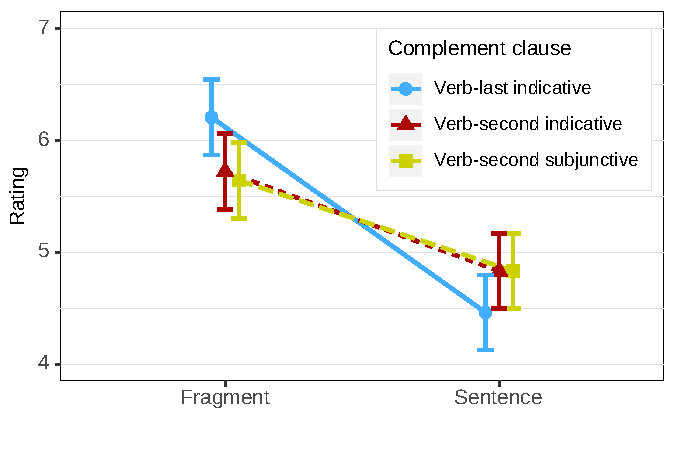
\includegraphics[scale=1]{figures/ex2b_ccs_de_lc_estimates}
 \caption{Mean ratings and 95\% confidence intervals across conditions in experiment \ref{exp:ccs-german}. \label{fig:ccs-german-estimates}}
\end{figure}
%
The data were statistically analyzed with CLMMs in \texttt{R} following the procedure described in Section \ref{sec:intro-stats}. Since \textsc{CCType} was a ternary factor, I first conducted an analysis on the data for verb-second CC\is{Complement clause}s only in order to test the conjecture that they did not differ significantly from each other. If this was confirmed, the two verb-second conditions could be pooled for further analysis and \textsc{CCType} treated as a binary predictor. The initial model for this analysis contained fixed effects for \textsc{CCType}, \textsc{Sententiality}, \textsc{Position} of the trial in the experiment and \textsc{MatrixVerb} in order to account for an effect of the verb's subcategorization preferences, as would be evidenced by a \textsc{MatrixVerb:CC\is{Complement clause}Type} interaction. As for random effects, I included by-subject and by-item random intercepts and random slopes for \textsc{Sententiality}, \textsc{MatrixVerb}, \textsc{CCType} and the interactions thereof.%
% 
\footnote{A by-subject random slope for \textsc{Sententiality} and the corresponding interactions were omitted as it would make no sense for a between subjects IV. Similarly, there was no by-item slope for \textsc{MatrixVerb} and interactions thereof, because \textsc{MatrixVerb} was not varied between items.}\afterfn%
%
Since the analysis of verb-second CCs\is{Complement clause} revealed no significant difference between subjunctive and indicative \clmmLRnonsig{0.19}{0.6} verb-second CCs, the verb-second conditions were pooled for further analysis. The full model fitted to the complete data set after pooling had the same effects structure as the model for verb-second CCs\is{Complement clause}.\largerpage

The final model is summarized in Table \ref{tab:ccs-german-estimates}. It contained significant main effects of both IVs and a significant interaction between them. The main effect of \textsc{Sententiality} \clmmLR{14.57}{0.001} confirms that fragments are rated\is{Acceptability rating task} better than left dislocations averaging over \textsc{CCType} conditions.%
%
\footnote{The significance of main effects of predictors that significantly interacted with others was assessed by the procedure described in \citet{levy2018}. I sum-coded the other predictor participating in the interaction and then compared a model that contains the predictor to be tested to one that does not with a likelihood ratio test.}\afterfn%
%
The main effect of \textsc{CCType} \clmmLR{6.02}{0.05} indicates that verb-last clauses were preferred over verb-second ones, and the significant \textsc{Sententiality:CC\is{Complement clause}Type} \clmmLR{25.75}{\highsig} interaction shows that this preference is specifically large for fragments. 
The \textsc{MatrixVerb} had no significant effect on acceptability and neither participated in any significant interaction. The significant main effect of \textsc{Position} \clmmLR{16.76}{\highsig} shows that items were perceived as more acceptable the later they appeared in the experiment, while the interaction with \textsc{Sententiality} \clmmLR{12.73}{0.001} suggests that this effect was stronger for fragments than for left dislocations. These predictors are not theoretically interesting, but their inclusion factors out the familiarization effects. 

\begin{table}
\begin{tabular}{l l l c c l}
\lsptoprule
Predictor & Estimate & SE & $\chi^2$ &  $p$ &  \\   
\midrule
\textsc{Sententiality}  & \phantom{-}0.834 &  0.231 &  14.57  &\textless 0.001 & ***\\
\textsc{CCType} & -0.19 &  0.067 & \phantom{1}6.02 &\textless 0.05\phantom{1} &* \\
\textsc{Position}   &   \phantom{-}0.009 &  0.002 &  16.76 & \textless \highsig & ***\\
\textsc{Sententiality:CC\is{Complement clause}Type} & -0.447 &  0.068 & 25.75 & \textless \highsig & ***\\
\textsc{Sententiality:Position}  &   \phantom{-}0.008 &  0.002 &  12.73 & \textless 0.001 & ***\\
\lspbottomrule
\end{tabular}
\caption{Fixed effects in the final CLMM for experiment \ref{exp:ccs-german}. \label{tab:ccs-german-estimates}}
\end{table}

In addition to the analysis of the complete data set, I performed an analysis of the sentential left dislocation conditions only in order to test the movement restriction\is{Movement restriction} on complementizer-less\is{Complementizer omission} CCs\is{Complement clause}. The full model had the same effects structure like the one in the main analysis, with the obvious exception that all effects for \textsc{Sententiality} were removed. The final model contained only a significant main effect of \textsc{CCType} \clmmLR{10.68}{0.01} evidencing that clauses headed by a complementizer were rated\is{Acceptability rating task} as significantly worse than their complementizer-less\is{Complementizer omission} counterparts.

\subsubsection{Discussion}
Experiment \ref{exp:ccs-german} investigated (i) whether fronting complementizer-less\is{Complementizer omission} CCs\is{Complement clause} is degraded as compared to CCs\is{Complement clause} headed by overt complementizers, and (ii) whether this movement restriction\is{Movement restriction} is reflected in the acceptability of fragments. 

The significant \textsc{Sententiality:CCType} interaction shows that the preference for realizing the complementizer\is{Complementizer omission} is stronger for fragments than for left dislocated CC\is{Complement clause}s. The analysis of the sentential conditions only shows that the preference for realizing the complementizer is even inverted in full sentences: In contrast to the claim by \citet{webelhuth1992}, who argues that this movement restriction\is{Movement restriction} is a property of ``all finite declarative argument clauses in the Germanic languages'' \citep[83]{webelhuth1992}, omitting the complementizer\is{Complementizer omission} is preferred in the full sentence. At least for German\il{German}, this undermines the reasoning upon which the interpretation of the data in \citet{merchant.etal2013} is based, since there is no evidence for a movement restriction\is{Movement restriction} on complementizer-less\is{Complementizer omission} CC\is{Complement clause}s. Furthermore, the sentential conditions seem to be grammatical across the board, as their mean ratings (for all conditions $\mu > 4.5$) are clearly above those for ungrammatical controls ($\mu = 2.4$). 

The fragment data alone resemble the pattern reported by \citet{merchant.etal2013}: Fragment CCs\is{Complement clause} are more acceptable when they are introduced by a complementizer than when they are not. However, since there is no evidence for the movement restriction\is{Movement restriction} stated in the literature, this effect cannot be attributed to constraints on movement. Furthermore, all three fragment conditions seem to be relatively acceptable, and even the dispreferred complementizer-less\is{Complementizer omission} fragments were rated\is{Acceptability rating task} much better than ungrammatical controls ($\mu = 2.18$). Unlike in the experiment by \citet{merchant.etal2013}, the explanation that they were interpreted as indirect answers is ruled out by the context story. Furthermore, there was no significant difference at all between subjunctive and indicative mood, even though the indirect answer interpretation is only possible in the indicative conditions. Since subjunctive encodes reported speech,  it cannot be interpreted as an indirect answer and they would have been preferred over indicative ones if the indirect answer explanation for the relatively high ratings for complementizer-less\is{Complementizer omission} CCs\is{Complement clause} in \citet{merchant.etal2013} was correct.

Taken together, the data indicate that, at least in German\il{German}, the preference for realizing the complementizer in short answer fragments\is{Fragment, short answer} observed by \citet{merchant.etal2013}, which my experiment replicates, seems not to be caused by a movement restriction\is{Movement restriction} on complementizer-less\is{Complementizer omission} CCs\is{Complement clause}. If this finding is robust and generalizes to English\il{English}, it would question the reasoning behind the experiment by \citet{merchant.etal2013}: If the movement restriction\is{Movement restriction} in question does not hold, no conclusions with respect to this can be drawn from the acceptability of the corresponding fragments. Experiment \ref{exp:ccs-english} will replicate this study in English\il{English} to investigate whether the difference between the results in \citet{merchant.etal2013} and my German\il{German} data evidences a cross-linguistic difference or whether it must be attributed to properties of the experiment design.

\subsubsection{Follow-up study with shorter contexts}

\subsubsubsection{Background and materials}
The stimuli tested in experiment \ref{exp:ccs-german} were relatively long and complex as compared to those used by \citet{merchant.etal2013}. Instead of a question-answer pair, they consisted of a context story and two turns per character. This might have biased subjects to base their ratings rather on the naturalness of the target utterance in discourse than on its grammaticality alone. In order to address this concern, I conducted a follow-up experiment using similar materials, but slightly longer context stories and two-turn dialogues which consisted only of the critical question-answer pair \Next.

\ex. [Context story] This weekend a famous painting has been stolen from the museum. The newscaster is reporting on the investigation of the robbery. The investigators are currently discussing how the burglar got into the building.\\\mbox{}[Newscaster:] Was glaubt Kommissar Wagner?\\\mbox{}[Reporter:]  Der Täter ist durch das Fenster eingestiegen(, glaubt er).

\subsubsubsection{Method}
The experiment was presented on the Internet using Lime\-Survey. Originally, it was conducted in the same session as the production study\is{Production task} on case marking (experiment \ref{exp:case-production}), where subjects were asked to produce utterances referring to graphical stimuli. The experiment was completed by 38 undergraduate students of Saarland University, who were rewarded with the participation in a lottery of 5 $\times$ \currencyEuro{30.00} among all participants.%
%
\footnote{Due to a technical problem, two out of the six lists (which included 10 subjects) were assigned experimental materials in the incorrect conditions. The corresponding participants were replaced by subjects recruited on the \textit{clickworker} crowdsourcing platform. These subjects rated\is{Acceptability rating task} the correct materials, which were mixed with the stimuli from experiment \ref{exp:mvb} and the same fillers as in the original lists. Each subject on the replacement lists was paid \currencyEuro{3.00} for participating. Since the distribution issue does not concern the stimuli of experiment \ref{exp:mvb}, in the case of experiment \ref{exp:mvb} I report the original data.}\afterfn%
%
The task and assignment to lists was identical to experiment \ref{exp:ccs-german} and \textsc{Sententiality} was tested between subjects again. Each subject rated\is{Acceptability rating task} 21 items (7 per \textsc{CCType} condition). Materials were presented together with 35 items of experiment \ref{exp:mvb} and 25 unrelated fillers including four ungrammatical controls in individually pseudo-randomized order. Pseudo-randomization ensured that no two items of the same experiment followed each other. One participant rated\is{Acceptability rating task} 50\% or more of the ungrammatical attention checks as acceptable (6 or 7 points on the scale) and was therefore excluded from further analysis.

\subsubsubsection{Results}
Figure \ref{fig:ccs-german-short-estimates} shows the aggregated ratings across conditions. The pattern is similar to experiment \ref{exp:ccs-german}, despite the slightly different ratings in absolute terms, which might be due to the differing materials that were tested together with the items in experiments \ref{exp:ccs-german} and the follow-up study.
%
\begin{figure}
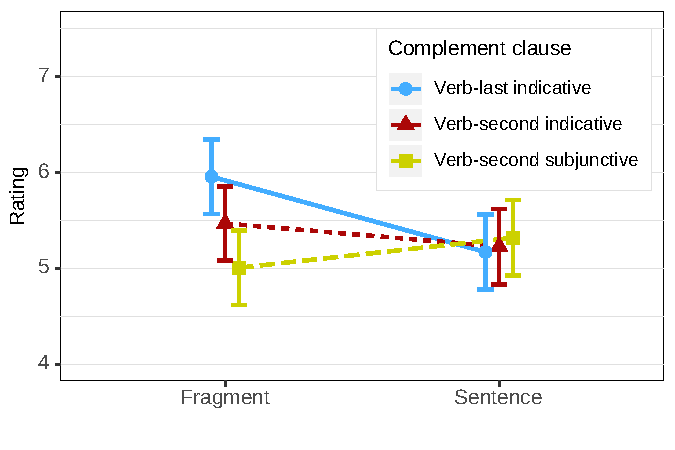
\includegraphics[scale=1]{figures/ex2b_ccs_de_sc_estimates}
 \caption{Mean ratings and 95\% confidence intervals across conditions in the follow-up to experiment \ref{exp:ccs-german}. \label{fig:ccs-german-short-estimates}}
\end{figure}
%
The statistical analysis followed the same procedure as for experiment \ref{exp:ccs-german}. First, pairwise analyses compared two of the three levels of \textsc{CCType} at a time. In all three analyses there were significant effects of \textsc{CCType} or significant interactions of \textsc{CCType} and \textsc{Sententiality}, therefore I did not pool the data. In all of the analyses, the full model contained main effects for \textsc{Sententiality}, \textsc{CCType} and \textsc{MatrixVerb} as well as all two-way interactions. I also included by-subject random intercepts and slopes for \textsc{CCType}, \textsc{MatrixVerb} and their interaction, as well as by-item random intercepts and slopes for \textsc{CCType}, \textsc{Sententiality} and their interaction. By-item random effects for \textsc{MatrixVerb} were not considered because the matrix verb was not varied between items. The same holds for by-subject \textsc{Sententiality} random effects.

First, I analyzed only the data for the indicative (verb-second and verb-last) complement clauses\is{Complement clause}. The final model is summarized in Table \ref{tab:ccs-short-indicative-modeltab}. A significant effect of \textsc{Sententiality} \clmmLR{12.64}{\highsig} evidences an overall preference for fragments over sentences with sentence-initial CCs\is{Complement clause}. The \textsc{Sententiality:CCType} interaction \clmmLR{7.16}{0.01} shows that in the case of fragments there is a preference for verb-last CCs\is{Complement clause} with overt complementizers, which however is not observed for sentences, since the main effect of \textsc{CCType} is not significant \clmmLRnonsig{1.67}{0.1}. The \textsc{MatrixVerb} did neither have a significant main effect nor did it interact with any of the other predictors.

\begin{table}
\begin{tabular}{l l l l l l}
\lsptoprule
Predictor & Estimate & SE & $\chi^2$ &  $p$ &  \\   
\midrule
\textsc{Sententiality} & \phantom{-}1.315 & 0.37 & 12.64 & \textless \highsig & ***\\
\textsc{CCType}   & -0.347 & 0.263 & \phantom{1}1.67 & \textgreater 0.1 &\\  
\textsc{Sententiality:CC\is{Complement clause}Type} & -1.289 & 0.472 & \phantom{1}7.16 & \textless 0.01 & **\\\lspbottomrule
\end{tabular}
\caption{Fixed effects in the final CLMM for the verb-second and verb-last indicative conditions in the follow-up to experiment \ref{exp:ccs-german}. \label{tab:ccs-short-indicative-modeltab}}
\end{table}

In a second analysis I compared only the indicative and subjunctive verb-second conditions. In this case, the only significant effect in the final model (see Table \ref{tab:ccs-short-v2-modeltab}) is an interaction of \textsc{Sententiality} and \textsc{Condition} \clmmLR{4.81}{0.05}: Subjunctive verb-second CCs\is{Complement clause} are significantly degraded as compared to indicative ones as fragments as compared to the left dislocation conditions. The effects of \textsc{Condition}  \clmmLRnonsig{1.681}{0.1} and \textsc{Sententiality} \clmmLRnonsig{0.01}{0.9} are not significant but kept in the model due to the significance of the interaction. Again, there were no effects of \textsc{MatrixVerb}.

\begin{table}
\begin{tabular}{l l l l l l}
\lsptoprule
Predictor & Estimate & SE & $\chi^2$ &  $p$ &  \\   
\midrule
\textsc{Sententiality} & \phantom{-}0.035 & 0.533 & 0.01 & \textgreater 0.9 &\\
\textsc{CCType}   & -0.45 & 0.343 & 1.681 & \textgreater 0.1 & \\  
\textsc{Sententiality:CC\is{Complement clause}Type}  & -1.201 & 0.535 & 4.81& \textless 0.05 & *\\\lspbottomrule
\end{tabular}
\caption{Fixed effects in the final CLMM for the indicative and subjunctive verb-second conditions in the follow-up to experiment \ref{exp:ccs-german}. \label{tab:ccs-short-v2-modeltab}}
\end{table}

Finally, I compared only the data for the subjunctive and the verb-last CCs\is{Complement clause}, which cannot be interpreted as indirect answers. The final model is summarized in Table \ref{tab:ccs-short-embedded-modeltab}. The significant effect of \textsc{CCType} \clmmLR{7.24}{0.01} shows that subjunctive CCs\is{Complement clause} are overall dispreferred as compared to verb-last CCs\is{Complement clause}. In this analysis, the overall preference for fragments is only marginal \clmmLRnonsig{2.8}{0.05}. Like in the analysis of the indicative data, the \textsc{Sententiality:CCType} interaction \clmmLR{22.33}{\highsig} shows that verb-last CCs\is{Complement clause} are particularly preferred as fragments. Again, there were no effects of \textsc{MatrixVerb}.

\begin{table}
\begin{tabular}{l l l l l l}
\lsptoprule
Predictor & Estimate & SE & $\chi^2$ &  $p$ &  \\   
\midrule
\textsc{Sententiality} & \phantom{-}0.579 & 0.345 & \phantom{2}2.8 & \textgreater 0.05 &\\
\textsc{CCType}   & -0.971 & 0.351 & \phantom{2}7.24 & \textless 0.01 & **\\  
\textsc{Sententiality:CC\is{Complement clause}Type}  &-2.543 & 0.53 & 22.33 & \textless \highsig & ***\\
\lspbottomrule
\end{tabular}
\caption{Fixed effects in the final CLMM for the verb-second indicative and the verb-last subjunctive conditions in the follow-up to experiment \ref{exp:ccs-german}. \label{tab:ccs-short-embedded-modeltab}}
\end{table}

\subsubsubsection{Discussion}
The follow-up study finds relatively similar results to experiment \ref{exp:ccs-german} with shorter contexts. Again, there is evidence for the preference for verb-last CCs\is{Complement clause} with overt complementizers that \citet{merchant.etal2013} report in fragments, but not in complete sentences. Unlike in experiment \ref{exp:ccs-german}, the subjunctive verb-second fragments were slightly degraded as compared to indicative verb-second fragments, but this effect is also not reflected in left dislocation structures in full sentences.

\refstepcounter{expcounter}\label{exp:ccs-english}
\subsection{Experiment \ref{exp:ccs-english}: CC topicalization in English}

\subsubsection{Background}
\begin{sloppypar}
Experiment \ref{exp:ccs-german} replicated the pattern reported by \citet{merchant.etal2013} for fragments but found no difference between the corresponding topicalized CCs\is{Complement clause}. This could either indicate a crosslinguistic difference between German\il{German} and English\il{English} or be due to the absence of the movement restriction\is{Movement restriction}. In order to distinguish between these explanations I conducted an English\il{English} version of experiment \ref{exp:ccs-german} that would show whether there is evidence for the presumed movement restriction\is{Movement restriction} on complementizer-less\is{Complementizer omission} CCs\is{Complement clause} or whether English\il{English} patterns with my German\il{German} data. Since there were no meaningful differences between the main experiment \ref{exp:ccs-german} and the follow-up, the shorter stimuli tested in the follow-up were used.
\end{sloppypar}

The predictions of movement and deletion\is{Movement and deletion account} are identical to experiment \ref{exp:ccs-german}: If the data in \citet{merchant.etal2013} are due to a movement restriction\is{Movement restriction}, complementizer-less\is{Complementizer omission} CCs\is{Complement clause} should be degraded both as fragments and in a left-peripheral position.

\subsubsection{Materials}\label{sec:ccs-english-materials}
The materials were in principle identical to those from experiment \ref{exp:ccs-german} and were translated into American English\il{English} by a native speaker. A sample item is given in \Next (context story) and \NNext (target utterances). The most important difference to the German\il{German} experiment was the omission of the subjunctive conditions, because in English\il{English} subjunctive does not have the same status as a marker of reported speech that it has in German\il{German}. This resulted in a 2$\times$2 design that crossed \textsc{CCType} (\textit{that} vs. null complementizers) with \textsc{Sententiality}. Again, \textsc{Sententiality} was tested as a between subjects IV. Besides reducing the likelihood of a floor effect, this allowed for a comparison with my German\il{German} studies and the original experiment by \citet{merchant.etal2013}. The English\il{English} verbs used in the matrix clause that embedded the CC\is{Complement clause} in the sentential conditions were \textit{to believe}, \textit{to think}, \textit{to say} and \textit{to mean}.

\ex. [Context story] This weekend a famous painting has been stolen from the museum. The newscaster is reporting on the investigation of the robbery. The investigators are currently discussing how the burglar got into the building.\\\mbox{}[Newscaster:] What does inspector Wagner believe?


\ex. [Reporter:]
\a. That the criminal entered through the window.
\b. The criminal entered through the window.
\c. The criminal entered through the window, he believes.
\d. That the criminal entered through the window, he believes.

\subsubsection{Procedure}\label{sec:ccs-english-method}
The experiment was completed by 54 native speakers of American English\il{English}, who were recruited on the \textit{Prolific Academic} crowdsourcing platform. The study was run over the Internet using the LimeSurvey presentation software. Each participant received \currencyPound{2} for participation. Subjects were asked to rate the naturalness of the italicized target utterance in the context of the question. They were assigned to one out of four lists. As \textsc{Sententiality} was tested between subjects, two of the lists contained only fragment and two only sentential target utterances. The materials were distributed across four lists according to a Latin square, so that each subject saw each token set once and each \textsc{CCType} condition equally often. 
Each subject rated\is{Acceptability rating task} 20 items (10 per \textsc{CCType} condition).%
%
\footnote{One of the German\il{German} materials ($n=21$) was not used in order to obtain an even number of materials.}\afterfn%
%
The stimuli were mixed with 20 items from experiment \ref{exp:pstranding-english} and 45 fillers. All fillers consisted of context stories which were followed by a dialogue. The target utterance was always the last utterance in that dialogue, and fillers were adapted so that participants assigned to the fragment lists rated\is{Acceptability rating task} only fragments and those assigned to the sentential lists only sentences. The stimuli were presented in individually fully randomized order. The fillers included five ungrammatical controls, which contained e.g. wrong auxiliaries or voice. Four subjects who rated\is{Acceptability rating task} more than 50\% with 6 or 7 points on the scale were excluded from further analysis.

\subsubsection{Results}\label{sec:ccs-english-results}

Figure \ref{fig:ccs-english-estimates} shows the aggregated ratings across conditions. The ratings for fragments are almost identical independently of the presence of a complementizer ($\mu_{that} = 5.69$, $\mu_{null} = 5.8$). This suggests that the effect reported by \citet{merchant.etal2013} was not replicated. Furthermore, topicalized CCs\is{Complement clause} without overt complementizers ($\mu_{null} = 3.98$), appear to be more acceptable than those headed by \textit{that} ($\mu_{that} = 3.08$), in contrast to the introspective data reported in the literature.

\begin{figure}
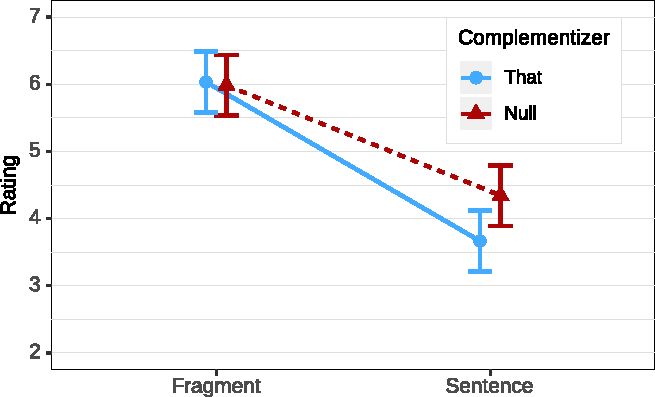
\includegraphics[scale=1]{figures/ex2b_ccs_en_estimates}
 \caption{Mean ratings and 95\% confidence intervals across conditions in experiment \ref{exp:ccs-english}. \label{fig:ccs-english-estimates}}
\end{figure}

The data were analyzed with CLMMs in \texttt{R} following the procedure described in Section \ref{sec:intro-stats}. I first fit a full model to the complete data set. The full model contained fixed effects for \textsc{Sententiality}, \textsc{CCType}, the \textsc{Position} of the trial in the time-course of the experiment and the \textsc{MatrixVerb} as well all two-way interactions between the IVs. The models had by-item random intercepts by-item random slopes for \textsc{Sententiality}, \textsc{CCType} and their interaction, as well as by-subject random intercepts and by-subject random slopes for \textsc{CCType}. By-subject random slopes for \textsc{Sententiality} were not considered, because \textsc{Sententiality} was tested as a between subjects IV. 

The final model (see Table \ref{tab:ccs-english-estimates}) contains significant main effects of \textsc{Sententiality}, \textsc{CCType}, \textsc{Position}, \textsc{MatrixVerb} and the \textsc{Sententiality:CC\is{Complement clause}Type} interaction. The main effect of \textsc{Sententiality} \clmmLR{29.85}{\highsig} confirms that fragments are preferred over topicalized CC\is{Complement clause}s. The main effect of \textsc{CCType} \clmmLR{10.58}{0.01} shows that, unlike it has been argued in the theoretical literature based on introspective data, complementizer omission\is{Complementizer omission} is overall preferred. Finally, the significant interaction between \textsc{Sententiality} and \textsc{CCType} \clmmLR{6.05}{0.05} shows that the preference for complementizer omission\is{Complementizer omission} is specifically strong for sentences. The \textsc{Position} effect \clmmLR{11.64}{0.001} reveals a slight overall improvement of ratings over time, but the absence of interactions with other predictors shows that this does not affect any condition in particular. The \textsc{MatrixVerb} main effect \clmmLR{7.6}{0.01} reveals a preference for materials with the matrix verb \textit{believe} as compared to other matrix verbs, for the other matrix verbs there was no such effect. Since the verb was not varied systematically across all items, this might be due to properties of individual materials, hence I consider this a control predictor. Just like in the German\il{German} experiments, I addressed the movement restriction\is{Movement restriction} with an analysis of the data for the full sentences only, following the same procedure as for the main analysis. The final model contains a \textsc{Position} effect \clmmLR{5.63}{0.05} and a main effect of \textsc{CCType} \clmmLR{13.7}{0.001} that confirms the preference for complementizer-less\is{Complementizer omission} clauses in a left-peripheral position.

\begin{table}
\begin{tabular}{l l l l l l}
\lsptoprule
Predictor & Estimate & SE & $\chi^2$ &  $p$ &  \\   
\midrule
\textsc{Sententiality} & \phantom{-}1.886 &  0.302 & 29.85 & \textless \highsig & *** \\
\textsc{CCType}  &  \phantom{-}0.443 &  0.13 & 10.58 & \textless 0.01 & ** \\
\textsc{MatrixVerb (believe)} &   \phantom{-}0.441 &  0.15  & \phantom{1}7.60 & \textless 0.01 & **\\ 
\textsc{Position}      &     \phantom{-}0.009 & 0.003   & 11.64 & \textless 0.001 & *** \\
\textsc{Sententiality:CC\is{Complement clause}Type} & -0.323 & 0.128  & \phantom{1}6.05 & \textless 0.05 & *\\
\lspbottomrule
\end{tabular}
\caption{Fixed effects in the final CLMM for experiment \ref{exp:ccs-english}. \label{tab:ccs-english-estimates}}
\end{table}

\subsubsection{Discussion}
Like experiment \ref{exp:ccs-german}, experiment \ref{exp:ccs-english} investigated an assumed movement restriction\is{Movement restriction} on complementizer-less\is{Complementizer omission} CCs\is{Complement clause} that constrains the acceptability of the corresponding fragments according to \citet{merchant.etal2013}. The data do neither provide evidence for the assumed movement restriction\is{Movement restriction} nor for the effect that \citet{merchant.etal2013} report for fragments. The overall pattern in my English\il{English} data is similar to that found for German\il{German}: Short answers\is{Fragment, short answer} are preferred across the board and the overall difference in acceptability between \textsc{CCType} conditions is rather small in absolute terms. In English\il{English}, there was no difference in acceptability between both types of fragment CCs\is{Complement clause}. This contrasts with the study by \citet{merchant.etal2013}, who found such an effect, and suggests that the preference for CCs\is{Complement clause} with overt complementizers in their experiment was due to the use of factive\is{Factivity} matrix verbs, which disprefer complementizer-less\is{Complementizer omission} CCs\is{Complement clause}. Once more, there is no evidence for the movement restriction\is{Movement restriction} on which the study by \citet{merchant.etal2013} is based: Complementizer-less\is{Complementizer omission} CCs\is{Complement clause} were even rated\is{Acceptability rating task} as more acceptable that in the sentential conditions, whereas the opposite pattern has been repeatedly assumed in the theoretical literature based on introspective data.

\subsection{General discussion: Complementizer omission}
\begin{sloppypar}
Experiments \ref{exp:ccs-german} and \ref{exp:ccs-english} investigated whether the presumed movement restriction\is{Movement restriction} on comple\-men\-tizer-less CCs\is{Complement clause} that \citet{merchant.etal2013} investigated indeed provides evidence for movement in fragments\is{Movement and deletion account}. The results suggest that it does not: First, there is no empirical evidence for the presumed movement restriction\is{Movement restriction} on complementizer-less\is{Complementizer omission} CCs\is{Complement clause}. Second, complementizer-less\is{Complementizer omission} CC\is{Complement clause} fragments are slightly degraded in German\il{German}, but this pattern is not reflected in the corresponding full sentences. In English\il{English}, there is no difference between fragments, and in full sentences the complementizer-less\is{Complementizer omission} CC\is{Complement clause} is even preferred. This suggests that \citet{merchant.etal2013} interpret their data based on incorrect assumptions and that the preference for realizing the complementizer in their materials is not related to movement restriction\is{Movement restriction}s.
\end{sloppypar}

The study by \citet{merchant.etal2013} differs from my experiments in three main aspects: First, the restriction to CCs\is{Complement clause} that are acceptable in situ, that is complements of non-factive verbs\is{Factivity}, ensures that a possible preference for complementizer realization cannot be explained by in situ deletion\is{In situ deletion account}. Degraded ratings for CCs\is{Complement clause} which are ungrammatical even in situ are expected by \textit{any} ellipsis account. Second, the use of context stories ruled out the possibility of indirect answers, and third, I collected ratings for the left dislocation structures that \citet{merchant2004} assumes to be the source of fragments. \citet{merchant.etal2013} simply relied on the movement restriction\is{Movement restriction} on complementizer-less\is{Complementizer omission} CCs\is{Complement clause} reported in the literature. 

In both experiments, topicalized CCs\is{Complement clause} were rated\is{Acceptability rating task} as worse than fragments across the board, even though \textsc{CCType} was tested within subjects in order to attenuate this effect. None of the experiments confirmed the pattern reported in the literature with respect to topicalized CCs\is{Complement clause}: Both in English\il{English} and German\il{German} there were significant \textsc{Sententiality:CCType} interactions showing that the preference for realizing the complementizer is stronger in fragments than in left dislocation structures. The analyses of the sentential conditions in isolation show that complementizer-less\is{Complementizer omission} clauses were rated\is{Acceptability rating task} as more acceptable in the left-peripheral position in English\il{English}, and at least as acceptable in German\il{German} (in the follow-up to experiment \ref{exp:ccs-german} there was no significant difference). This is the opposite pattern to the one reported in the theoretical literature that underlies the interpretation of the data in \citet{merchant.etal2013}. If complementizer-less\is{Complementizer omission} CCs\is{Complement clause} are not dispreferred in a left-peripheral position, the preference for realizing the complementizer in fragments cannot be attributed to a movement restriction\is{Movement restriction}: No matter why we observe this pattern in fragments, it does not provide evidence for movement.

Rebecca Woods\ia{Woods, Rebecca} (p.c.) pointed out the possibility that the ratings for topicalized complementizer-less\is{Complementizer omission} CCs\is{Complement clause} improved because they were interpreted as parentheticals rather than as matrix clauses. Parentheticals do not subcategorize the embedding clause but can be inserted into regular verb-second clauses, hence it should be possible to omit the complementizer in that case. However, in the German\il{German} subjunctive conditions, which did not differ in acceptability\is{Acceptability rating task} from indicative, subjunctive mood marks the utterance as indirect speech. Since indirect speech is in general embedded under a matrix verb, a parenthetical reading of the matrix clause seems less appropriate in that case than with regular indicative verb-second clauses. If the indicative verb-second fragments were improved by the parenthetical interpretation, subjunctive should be to a lesser extent and hence rated\is{Acceptability rating task} worse. This is clearly not the case. In order to be completely sure however, the items would have to be modified in a way that rules out the parenthetical reading, for instance by including a negation in the matrix clause.

When only fragments are taken into account, the German\il{German}, but not the English\il{English}, data resemble those reported by \citet{merchant.etal2013}, even when controlling for factivity\is{Factivity}. In both German\il{German} experiments realizing the complementizer was preferred, whereas there was no significant effect of the complementizer on English\il{English} fragments. The difference in acceptability between conditions is smaller than in the experiment by \citet{merchant.etal2013} in absolute terms even though I used a 7-point scale instead of a 5-point scale. This might be due to the restriction to non-factive\is{Factivity} verbs, which are known to allow for complementizer omission\is{Complementizer omission}. Even though the results on sentence-initial CCs\is{Complement clause} do not evidence a movement restriction\is{Movement restriction}, a possible difference between German\il{German} and English\il{English} with respect to complementizer omission\is{Complementizer omission} might be investigated in future research.

Like the preposition omission\is{Preposition omission} data discussed in the previous section, my results do not \textit{falsify} the movement and deletion\is{Movement and deletion account} account. However, they challenge the interpretation of a relatively weak preference for realizing complementizers in short answer fragments\is{Fragment, short answer} when the experiment is replicated under more carefully controlled conditions as evidence for movement. The movement and deletion\is{Movement and deletion account} account can of course derive both fragment CCs\is{Complement clause} with and without complementizers from the corresponding left dislocations, which, unlike as has been argued in the literature, seem to be well-formed. However, there is no empirical evidence for the movement restriction\is{Movement restriction} assumed by \citet{merchant2004} and \citet{merchant.etal2013} that constrains the form of fragments. Therefore, even if the pattern predicted by \citet{merchant2004} is observed in some fragments (as it was by \citet{merchant.etal2013} and in experiment \ref{exp:ccs-german}), this cannot be traced back to a movement restriction\is{Movement restriction} on complementizer-less\is{Complementizer omission} complement clauses\is{Complement clause}. Since the movement and deletion\is{Movement and deletion account} account is derivationally more complex than in situ deletion\is{In situ deletion account}, the absence of evidence for movement forces us to stick to the simpler in situ deletion\is{In situ deletion account} account. If there is no movement restriction\is{Movement restriction} on complementizer-less\is{Complementizer omission} CCs\is{Complement clause}, this phenomenon may simply be the wrong testing ground for the movement and deletion\is{Movement and deletion account} account. For this reason, in Section \ref{sec:mvb} I explore whether a well-documented restriction on German\il{German} prefield\is{Prefield} configurations constrains the form of fragments.

\section{Movement restrictions: The German prefield}\label{sec:mvb}
\subsection{The German prefield and movement in fragments}
The replications and extensions of the experiments by \citet{merchant.etal2013} question the assumption that preposition omission\is{Preposition omission} and complement clause\is{Complement clause} topicalization provide evidence for movement\is{Movement and deletion account}. In the case of preposition omission\is{Preposition omission}, the data can be explained without assuming movement by question-answer parallelism, and for complement clause\is{Complement clause} topicalization, there is no evidence for the presumed movement restriction\is{Movement restriction} itself. This section presents a last experiment on the syntax of fragments that investigates a well-documented movement restriction\is{Movement restriction} concerning the prefield\is{Prefield} position in German\il{German}. In a nutshell, the idea is that if the preverbal position in German\il{German} verb-second sentences is analyzed as the landing site for fragments, as \citet{merchant2004} suggests, only those constituents that can appear in this position are possible fragments.

\subsubsection{The prefield position in German verb-second clauses}
The German\il{German} declarative matrix clause is generally assumed to be strictly verb-second, so that only one constituent can precede the inflected verb. \is{Topological field model|(}Traditionally, this is modeled with the \textit{topological field model}\is{Topological field model} \citep{drach1937} of the German\il{German} sentence, which divides the sentence into three regions, the so-called \textit{fields}. These fields are delimited by two positions hosting verbal elements, the left and right \textit{brackets}. Table \ref{tab:feldermodell} shows how these fields are filled in declarative matrix clauses: The left bracket hosts the inflected verb and the right bracket the participle or infinitive, if the sentence contains such. The region left to the left bracket is called prefield\is{Prefield} and contains exactly one constituent, yielding the obligatory verb-second order. By default\is{Default case}, all other constituents appear in the middle field\is{Middle field}, the region between the brackets. In case of extraposition, constituents can be located in the postfield, i.e. in the region following the right bracket. \Next shows that, unlike in SVO languages, all arguments (including the subject) appear in the middle field\is{Middle field} if the prefield\is{Prefield} is filled by an adverbial\is{Adverbial}.\is{Topological field model|)}

\begin{table}
\begin{tabular}{l l l l l l l l}
\lsptoprule
Prefield & LB & \multicolumn{2}{c}{Middle field} & RB & \multicolumn{3}{c}{Postfield}  \\   
\midrule
Peter & will & einen & Kuchen & backen & der & glutenfrei & ist\\
Peter & wants & a & cake & bake & that & gluten.free & is\\
\lspbottomrule
\end{tabular}
\caption{German topological fields model (LB = left bracket; RB = right bracket).\label{tab:feldermodell}}
\end{table}

\exg. Montag will Peter [einen Kuchen] backen, [der glutenfrei ist].\\
monday wants Peter a cake bake that gluten.free is\\
\trans{On Monday, Peter wants to bake a cake that is gluten-free.}

In generative\is{Generative grammar} terms, the standard syntactic analysis of German\il{German} verb-second sentences assumes head movement of the verb from T to C followed by movement of the prefield\is{Prefield} constituent to [Spec, CP\is{Complementizer phrase}], as sketched in Figure \ref{ex:vorfeld-adv}.%
%
\footnote{This description is highly simplified. Furthermore, both the order of the movement operations and their motivation and casual connection (does one of them trigger the other, and if so, which?) have been controversially discussed (see \citet{brandner2004} for an overview of competing analyses of V2). In fact, Gereon \citet{muller2004} has argued that verb-second order is derived by remnant movement of the whole \textit{v}P to [Spec, CP\is{Complementizer phrase}] after the other constituents than the verb and the prefield\is{Prefield} constituents have been moved out for independent reasons. The resulting structure is given in \Next, taken from \citep[181]{muller2004}.

\ex. [\textsubscript{CP}\is{Complementizer phrase} [\textsubscript{vP}\textsubscript{5} Das Buch\textsubscript{2} \textit{t}\textsubscript{1} \textit{t}\textsubscript{4} hat\textsubscript{3} ] [\textsubscript{C'} C [\textsubscript{TP} Fritz\textsubscript{1} [\textsubscript{T'} [\textsubscript{VP}\textsubscript{4} \textit{t}\textsubscript{2} gelesen ] [\textsubscript{T'} \textit{t}\textsubscript{5} T]]]]]

\citeauthor{muller2004}'s account is not compatible with \citepos{merchant2004} version of movement and deletion\is{Movement and deletion account}. The E feature\is{E feature} on C would always cause the complete \textit{v}P to survive ellipsis, so that there would be no way of generating DP\is{Determiner phrase} fragments in German\il{German}. The corpus\is{Corpus} data by \citet{reich2017} and my previous experiments disconfirm this prediction. Note that this does not speak against \citeauthor{muller2004}'s analysis, unless movement and deletion\is{Movement and deletion account} is assumed.}\afterfn%
%

\begin{figure}
 \Tree [.CP Montag\textsubscript{j} [.C' will\textsubscript{i} [.TP \edge[roof]; {Peter \textit{t}\textsubscript{j} einen Kuchen backen [\dots] \textit{t}\textsubscript{i}} ] ] ] 
 
 \caption{Following \citet{denbesten1989}, the verb-second word order of the German declarative matrix clause is the result of moving the inflected verb to C and another constituent to [Spec, CP].\label{ex:vorfeld-adv}}
\end{figure}

\subsubsection{The prefield position in the movement and deletion account}\label{sec:mvb-merchant}
\is{Complementizer omission|(}
In order to draw conclusions on the validity of the movement and deletion\is{Movement and deletion account} account from prefield\is{Prefield} configurations, it is crucial to assume that movement in fragments\is{Movement and deletion account} really targets the prefield\is{Prefield} according to \citeauthor{merchant2004}'s account. The structure in Figure \ref{ex:vorfeld-adv} differs from the one that \citet{merchant2004} assumes for English\il{English} because C and [Spec, CP]\is{Complementizer phrase} are always filled in regular German\il{German} declarative matrix sentences. In contrast, English\il{English} declarative matrix sentences are TPs\is{Tense phrase}, and the C head hosting E\is{E feature} is phonologically empty. Therefore, it is not immediately clear which position \citeauthor{merchant2004} identifies as the landing site for fragments in German\il{German}. In principle there are three options: First, like \citeauthor{merchant2004} suggested for English\il{English}, there could be an FP above CP\is{Complementizer phrase} and the E feature\is{E feature} could be located on C. Second, there could be an FP above CP\is{Complementizer phrase} and the E feature\is{E feature} be hosted by F. Finally, there could be no FP in German\il{German}, but an E feature\is{E feature} located on C that triggers movement of fragments to [Spec, CP]\is{Complementizer phrase}. All of these options are compatible with the theory, because \citet{merchant2004} suggests to account for crosslinguistic differences with respect to the availability and properties of ellipses by postulating differences in the specifications of the lexicon entries of the E feature\is{E feature}. 

For the German\il{German} verb-second clause, as the discussion in Section \ref{sec:theories-predictions-focus} showed, any analysis that locates the E feature\is{E feature} on C incorrectly predicts that the inflected verb survives ellipsis, because it is moved to C and only the complement of C is PF-deleted.%
%
\footnote{Note that this problem also concerns the exceptional movement\is{Exceptional movement account} version of the theory by \citet{weir2014}. \citeauthor{weir2014} can account better for the non-constituent fragments discussed in this section, because he simply adjoins\is{Adjunct} fragments to CP\is{Complementizer phrase} and there is no upper bound on the number of adjuncts. There might be constraints on the order of constituents in fragments, depending on whether the most deeply embedded focused constituents or the closest ones to the E feature\is{E feature} are fronted first. However, \citeauthor{weir2014} places the E feature\is{E feature} on C and consequently falsely predicts that finite verbs (which are also in C), as Figure \ref{ex:vorfeld-adv} shows, always survive ellipsis.}\afterfn%
%
In contrast, assuming an FP above CP\is{Complementizer phrase} and locating E\is{E feature} on F has the advantage of deleting the verb and thus being able to generate DP\is{Determiner phrase} fragments. However, it incorrectly predicts fragments to be insensitive to island\is{Island}s, because the defective trace\is{Trace (movement)} in [Spec, CP\is{Complementizer phrase}] would be deleted along the way. As for the third option, the assumption of an FP in German\il{German} lacks empirical support, because the prefield\is{Prefield} hosts only one constituent and fronted foci appear in the regular prefield\is{Prefield} \Next[a] instead of preceding other prefield\is{Prefield} constituents \Next[b]. If no FP is assumed in German\il{German}, this rules out the first two options listed above.

\ex. \ag. \textit{Einen Topf} musst du nehmen, keine Pfanne!\\
	  a.\textsc{acc} pot must you take no pan\\
      \bg. *\textit{Einen Topf}  du musst nehmen, keine Pfanne!\\
	  a.\textsc{acc} pot you must take no pan\\
	  \trans{A pot you must take, not a pan!}
	 
Furthermore, the identification of the landing site for fragments as [Spec, CP\is{Complementizer phrase}] is also implicitly adopted by \citet{merchant2004} himself. As I discussed in Section \ref{sec:theories-predictions-focus}, \citet[702]{merchant2004} presents parallelisms between the form of fragments in the prefield\is{Prefield} and in fragments as evidence for his account. This  implies that the presumed landing site for fragments is the regular prefield\is{Prefield}, that is, [Spec, CP\is{Complementizer phrase}].\is{Complementizer omission|)}

\refstepcounter{expcounter}\label{exp:mvb}
\subsection{Experiment \ref{exp:mvb}: Multiple prefield constituents}
\subsubsection{Background}\label{sec:mvb-background}
The German\il{German} prefield\is{Prefield} is a promising testing ground for movement and deletion\is{Movement and deletion account}: Since \citet{merchant2004} assumes it to be the landing site for fragments, only those expressions that can appear there in regular sentences can be grammatical fragments. Experiment \ref{exp:mvb} tested this hypothesis using the same method as in the experiments on CC\is{Complement clause} topicalization, i.e. by comparing the acceptability of fragments to that of the corresponding left dislocation structures.

Testing this prediction empirically requires establishing which expressions can and which ones cannot appear in the prefield\is{Prefield}. Since the prefield\is{Prefield} can be filled with most of the syntactic categories,%
%
\footnote{Only few expressions, such as modal particles, cannot appear there, as \Next shows.

\exg.*Wohl\textsubscript{i}/Ja\textsubscript{i} hat Peter \textit{t}\textsubscript{i} ein paar Leute eingeladen.\\
\textsc{prt} has Peter \mbox{} a few people invited\\
\trans{Peter has probably invited a few people.}\exsourceraised{\citep[227]{ott.struckmeier2016}}

}\afterfn%
%
the main restriction is that only a single constituent can precede the verb, because there is only one landing site in [Spec, CP\is{Complementizer phrase}]. In fact, the possibility of fronting an expression in verb-second clauses is often used as a constituency test in German\il{German}. 

Despite this, a corpus\is{Corpus}-based collection of multiple prefield\is{Prefield} constituents by Stefan Müller \citep{muller2002, muller2003, muller2005} shows that, at least superficially, the requirement of German\il{German} declarative matrix clauses to be verb-second is frequently violated. Three examples from \citet[32, 38, 59]{muller2003} are given in \Next. Some of these examples can probably be analyzed as single constituents, depending on the theoretical background that is assumed. However, in \Last[a], it seems odd to adjoin\is{Adjunct} a sentential adverb\is{Adverbial} to a DP\is{Determiner phrase}%
%
\footnote{But see \citet{bogal-allbritten2013} for an account of how modal adverbials\is{Adverbial} modify DPs\is{Determiner phrase}.}\afterfn%
%
and is it also not immediately clear that the locative and temporal adverbials\is{Adverbial} in \Last[b] are simply adjoined\is{Adjunct} to each other, as suggested by \citet{haider2000}. \Last[c] can be analyzed as VP\is{Verb phrase} fronting following movement of the verb to T or C, depending on where the adverbial \textit{des öfteren} is placed.%
%
\footnote{
\citeauthor{muller2003} excludes some apparent multiple prefield\is{Prefield} constituents from the set of problematic cases. For instance, \citet[21]{muller2003} argues that in \Next \textit{den Wagen} and \textit{zu reparieren} are not independent from each other, as accusative\is{Accusative case} on \textit{den Wagen} has to be licensed by the verb \textit{reparieren}. Therefore, what is fronted is a complete verbal projection and not two independent constituents. 

\exg. Den Wagen zu reparieren wurde versucht.\\
      the car to repair was tried\\
      \trans{It was intended to repair the car.} \exsourceraised{\citep[21]{muller2003}}

}\afterfn%
%
In fact, \citet[13--22]{muller2005} himself argues that such prefield\is{Prefield} configurations constitute a single constituent headed by a phonologically null verb. 

\ex. \ag. [Vermutlich] [vom    gleichen  Täter]    wurden zwei Tankstellen in Hemsbach und Heidelberg überfallen.\\
probably of.the  same criminal were two gas.stations in Hemsbach and Heidelberg assaulted\\
\trans{Probably by the same criminal two gas stations in Hemsbach and Heidelberg were assaulted.}
\bg. [Vor drei  Wochen] [in Memphis] hatte Stich noch in drei Sätzen gegen Connors verloren.\\ 
before three weeks    in Memphis  had   Stich  still   in three sets   against Connors lost\\
\trans{Three weeks ago in Memphis Stich had still lost in three sets against Connors.}
\cg. [Studenten] [einem Lesetest] unterzieht er des öfteren.\label{ex:muller-vf-doio} \\ 
students a reading.test  submits he the more.frequent\\
\trans{Students a reading test he submits frequently.}

From the perspective of an empirical investigation of movement and deletion\is{Movement and deletion account} however, it is irrelevant how apparent multiple prefield\is{Prefield} constituents are analyzed: If the German\il{German} prefield\is{Prefield} is the landing site for fragments, the movement and deletion\is{Movement and deletion account} account predicts that only those expressions that can somehow be moved there are possible fragments. Experiment \ref{exp:mvb} tests this prediction by comparing three instances of multiple prefield\is{Prefield} configurations that \citet{muller2003} classifies as acceptable to two of those he argues that are ungrammatical. Again, these prefield\is{Prefield} configurations are tested both as fragments and in sentences.

\subsubsection{Materials}\label{sec:mvb-method}

Experiment \ref{exp:mvb} investigates five different prefield\is{Prefield} configurations in an acceptability rating\is{Acceptability rating task} study. Since multiple prefield\is{Prefield} configurations are restricted to specific information-structural\is{Information structure} contexts \citep{muller2005, bildhauer2011}, all critical utterances were preceded by a context that elicited the appropriate information structure\is{Information structure}. For instance, in  \Next, where both the direct and indirect object are fronted, \citet[59]{muller2003} notes that the first prefield\is{Prefield} constituent \textit{seinem Chef} `his boss' must be a contrastive topic\is{Topic, contrastive} \citep{buring1997} and the second one \textit{eine E-Mail} `an e-mail' a contrastive focus\is{Focus, contrastive}. 
The context question in \Next[a] intended to rule out the possibility that the utterance is inappropriate in out-of-the-blue contexts by information-structural\is{Information structure}ly licensing the marked word order\is{Word order}. Each item was tested as a fragment \Next[b] and in the prefield\is{Prefield} of a full sentence \Next[c].

\ex. Direct and indirect object \label{ex:mvb-item-doio}
\ag. Hätte  er  der Personalabteilung ein Fax schicken sollen?\\
has.\textsc{sbjv} he the HR.department a fax send shall\\
\trans{Should he have sent a fax to the HR department?}
\bg. Nein, seinem Chef eine E-Mail.\\
    no  his  boss an  e-mail\\
    \trans{No, his boss an e-mail.}
\cg. Nein, seinem Chef eine E-Mail hätte er schicken sollen.\\
	no his boss an  e-mail   has.\textsc{sbjv} he send shall\\
\trans{No, his boss an e-mail he should have sent.}

The experiment tested three prefield\is{Prefield} configurations that are grammatical according to \citet{muller2005} (direct + indirect object \Last, local + temporal adverbial\is{Adverbial} \ref{ex:mvb-item-loctemp} and argument + sentential adverb \ref{ex:mvb-item-sadvxp}) and two that are not (subject + other argument DP\is{Determiner phrase} \ref{ex:mvb-item-subjxp} and non-clausemates \ref{ex:mvb-item-diffcl}). Some of these conditions might be analyzed as involving a single constituent in the prefield\is{Prefield}: The cooccurrence of a locative and a temporal adverbial\is{Adverbial} \ref{ex:mvb-item-loctemp} could be analyzed as adjoined\is{Adjunct} to each other, but semantically both modify the remaining clause and not one of them the other one. In the sentential adverb and argument condition \NNext, the adverb\is{Adverbial} \textit{angeblich} `allegedly' takes scope over \textit{in seiner Stammkneipe} `in his favorite pub' only. This might indicate that it forms a constituent with the noun or DP\is{Determiner phrase}. \citet[31]{muller2003} nevertheless cites \ref{ex:muller-jacobs} by \citet[112]{jacobs1986} for evidence that sentential adverbs cannot occur inside a PP\is{Preposition phrase}. This indicates that they may be semantically associated with the noun, but not syntactically. After all, the purpose of the experiment is not to isolate prefield\is{Prefield} configurations that are equally acceptable but to investigate whether acceptability differences among them are reflected in the acceptability of fragments.

\ex. Locative and temporal adverbial\is{Adverbial}\label{ex:mvb-item-loctemp}
\ag. Wann hast  du   Hans denn getroffen? \\
when have you Hans  then  met\\
\trans{So when did you meet Hans?}
\bg. [Heute morgen  in der U-Bahn] habe ich ihn getroffen.\\
today   morning in the subway  have I    him met\\
\trans{This morning in the subway I met him.}

\ex. Sentential adverb\is{Adverbial} and argument XP\label{ex:mvb-item-sadvxp}
\ag. Wo  war Herr Veit zum   Tatzeitpunkt?\\
    where  was Mr    Veit to.the time.of.crime\\
\trans{Where was Mr Veit at the time of the crime?}
\bg. [Angeblich in seiner  Stammkneipe] war er  zum  Tatzeitpunkt.\\
allegedly in his favorite.pub was he to.the time.of.crime\\
\trans{Allegedly in his favorite pub he was at the time of the crime.}

\exg. *Peter träumt von (vermutlich/ sogar/ nicht) (ihr/ Luise/ Geld).\\  
 Peter dreams of probably/ even/ not her/ Luise/ money\\
\trans{Peter dreams of probably/even/not her/Luise/money.}\label{ex:muller-jacobs}

The two ungrammatical prefield\is{Prefield} configurations are given in \Next and \NNext. As for \Next, \citet[59]{muller2003} notes that a preverbal subject and an additional argument cannot appear together in the prefield\is{Prefield}. The ungrammatical configuration in \NNext involves the extraction of two constituents from different clauses to the prefield\is{Prefield}. This violates the requirement of prefield\is{Prefield} constituents to be clause-mates \citep{fanselow1993}. In \NNext, \textit{den Hund} `the dog' is the direct object of the embedded verb \textit{ärgern} `to bother', while \textit{Paul} is the indirect object of the matrix verb \textit{verbieten} `to forbid'. Note that, unlike in \Next, there is no subject involved in the multiple prefield\is{Prefield} sequence in \NNext. The prefield\is{Prefield} configuration itself should thus be acceptable if the constituents were not extracted from different clauses, as in \ref{ex:mvb-diffcl-nondiff}, because it consists of the direct and the indirect object like the presumably grammatical \ref{ex:mvb-item-doio}.

\ex. Subject and argument XP \label{ex:mvb-item-subjxp}
\ag. Wer möchte welche Aufgabe übernehmen? \\
    who wants   which   task        take.on\\
	\trans{Who wants to take on which task?}
	\bg. *[Ich die Spülmaschine] möchte übernehmen.\\
   I  the dishwasher   want     take.on \\
	\trans{I want to take on the dishwasher.}
	
\ex. Extraction out of different clauses \label{ex:mvb-item-diffcl}
\ag. Wem   hast  du   verboten, wen zu ärgern?\\
    whom  have you forbidden who to  bother\\
	\trans{Who did you forbid to bother who?}
	\bg. *[Paul den Hund] habe  ich verboten, zu ärgern.\\
     Paul   the  dog     have  I     forbidden to bother\\
	\trans{I forbade Paul to bother the dog.}
	
\exg. Paul den Hund habe ich geschenkt. \label{ex:mvb-diffcl-nondiff}\\
    Paul the  dog    have I    given.as.present\\
   \trans{I gave Paul the dog (as present).}

It shall be noted that \citet[710--711]{merchant2004} briefly discusses the (introspective) observation that short answer fragments\is{Fragment, short answer} to multiple \textit{wh}-questions are relatively acceptable even though the corresponding multiply filled prefield\is{Prefield} is heavily degraded. Without going into details, he suggests that this also evidences repair effects by ellipsis. I address this in the discussion of this experiment.

\subsubsection{Procedure}
The experiment was completed by 38 undergraduate students of Saarland University. All were native speakers of German\il{German}. They were rewarded with the participation in a lottery of 5 $\times$ \currencyEuro{30.00} among all participants. The experiment was conducted in the same session as the production study\is{Production task} on case marking (experiment \ref{exp:case-production}), where subjects were asked to produce utterances referring to graphical stimuli. Subjects were asked to rate the naturalness of the italicized target utterance in the context of the question on a 7-point Likert scale (7= fully natural). In order to prevent possible floor effects, \textsc{Sententiality} was tested as a between subjects variable. Each subject rated\is{Acceptability rating task} 35 items (7 per \textsc{Prefield}\is{Prefield} configuration). The materials were presented together with 21 items of the follow-up to experiment \ref{exp:ccs-german} and 25 unrelated fillers including four ungrammatical controls in individually pseudo-randomized order. A pseudo-randomized presentation ensured that no two items of the same experiment followed each other. Fillers were adapted so as to match the \textsc{Sententiality} of the materials in the list, so that subjects saw either only sentential or only fragment target utterances. This also matched the design of the follow-up to experiment \ref{exp:ccs-german}, which had the same manipulation. One participant rated\is{Acceptability rating task} 50\% or more of the ungrammatical controls with 6 or 7 points on the scale and was therefore excluded from further analysis. 

\begin{figure}
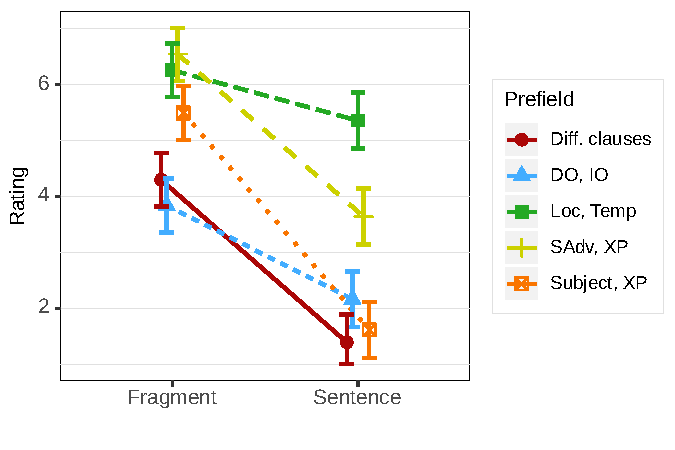
\includegraphics[scale=1]{figures/ex3_mvb_estimates}
 \caption{Mean ratings and 95\% confidence intervals across conditions in experiment \ref{exp:mvb}.\label{fig:mvb-estimates}}
\end{figure}

\subsubsection{Results}\label{sec:mvb-results}
Figure \ref{fig:mvb-estimates} shows that across all conditions fragments were rated\is{Acceptability rating task} better than sentences and that there was a large extent of variation between conditions. Specifically, the presumably ungrammatical conditions and grammatical conditions do not behave uniformly: The grammatical \textsc{SAdv, XP} and the grammatical \textsc{LocAdv, TempAdv} are both almost equally acceptable as fragments, but strongly differ as prefield\is{Prefield} configurations. Due to these differences, it would not be appropriate to pool the presumably ungrammatical and grammatical conditions. Instead, I conducted pairwise comparisons between each two of the conditions, yielding a series of 10 2$\times$2 contrasts (\textsc{Sententiality}$\times$\textsc{Prefield}) that I analyzed separately. For each of these contrasts I statistically analyzed a subset of the data containing only those data points belonging to the respective condition with CLMMs according to the procedure described in Section \ref{sec:intro-stats}.

\begin{table}
  \begin{tabular}{p{2cm} p{2cm}p{2cm}p{2cm}p{2cm}p{2cm}}
   \lsptoprule
   & \textsc{Subj, XP} & \textsc{SAdv, XP} & \textsc{Loc, Temp} & \textsc{DO, IO}\\
      \midrule
  \textsc{Non-CM}  & n.s. & n.s. & \clmmLRbr{11.52}{0.001} & \clmmLRbr{15.77}{\highsig} \\
  \textsc{DO, IO}  & \clmmLRbr{15.73}{\highsig} & \clmmLRbr{10.95}{0.001} & n.s. & \greycell \\
  \textsc{Loc, Temp} & \clmmLRbr{14.66}{0.001} & \clmmLRbr{11.32}{0.001} & \greycell  & \greycell \\
  \textsc{SAdv, XP} &  n.s.\linebreak~~ & \greycell & \greycell& \greycell \\
  \lspbottomrule
 \end{tabular}
\caption{Significance of the pairwise comparisons between prefield configurations. $p$-values were Bonferroni-corrected, i.e. multiplied by the number of comparisons ($n = 10$).\label{tab:mvb-interactions}}
\end{table}

The initial model for each data set contained main effects for \textsc{Sententiality} and \textsc{Prefield}\is{Prefield} as well as the interaction between these predictors. As for by-subject random effects I included only the intercept and a slope for \textsc{Prefield}\is{Prefield}, since \textsc{Sententiality} had been tested between subjects. Similarly, I included by-item random intercepts and slopes for \textsc{Sententiality}, because \textsc{Prefield}\is{Prefield} was not varied between items. The crucial predictor is the \textsc{Sententiality:Prefield}\is{Prefield} interaction, which indicates that the difference between conditions cannot be explained solely by a theoretically uninteresting overall preference for fragments or the markedness of a specific construction. Since the movement and deletion\is{Movement and deletion account} account predicts that only those prefield configurations which are acceptable as such yield grammatical fragments, it predicts no such interactions.

Table \ref{tab:mvb-interactions} summarizes the pairwise comparisons. Due to multiple comparisons, the reported $p$-values were Bonferroni-corrected, that is, multiplied by the number of comparisons ($n=10$). First of all, in most of the pairwise comparisons there are significant \textsc{Sententiality:Prefield}\is{Prefield} interactions. The pattern in Table \ref{tab:mvb-interactions} suggests that there is a split between conditions, but that this split does not occur between those prefield configurations that are grammatical and those that are ungrammatical according to \citet{muller2003}. The \textsc{Sententiality:Prefield}\is{Prefield} interactions are significant for any comparison between \textsc{Loc, Temp} and \textsc{DO, IO} and the remaining three predictors, but not between these two predictors. There are no significant interactions in the comparisons between the other three predictors. This suggests that the preference for the fragment is stronger in the two presumably ungrammatical prefield conditions and in \textsc{SAdv, XP}.

\subsubsection{Discussion}\label{sec:mvb-discussion}
Experiment \ref{exp:mvb} tested whether movement restrictions\is{Movement restriction} on German\il{German} multiple prefield\is{Prefield} configurations, which have not been investigated from this perspective previously, constrain the form of fragments. The idea underlying the experiment is that, if the movement and deletion\is{Movement and deletion account} account is correct, only those expressions that may appear in the preverbal position in German\il{German} verb-second clauses yield acceptable fragments. Statistically, this would be reflected in the absence of \textsc{Sententiality:Prefield} interactions between conditions.

As Table \ref{tab:mvb-interactions} shows, however, there are significant interactions in six out of ten pairwise comparisons. These interactions are unexpected under a movement and deletion\is{Movement and deletion account} account, but they do not ultimately falsify it, because some of the data points are close to the extremes of the scale and thus could reflect ceiling and floor effects, respectively. However, there are three conditions which are close to the mean rating for ungrammatical controls ($\mu = 1.79$) for sentences and ($\mu = 2.25$) for fragments,%
\footnote{\textsc{Sententiality} was tested between subjects, so that I present separate mean ratings for ungrammatical controls in each of the two groups.}\afterfn%
%
and among these specifically the \textsc{Subj, XP} condition yields acceptable fragments.

These interactions arise specifically when comparing the presumably grammatical prefield\is{Prefield} conditions (which involve the fronting of at least one adverbial\is{Adverbial}) to the ungrammatical ones (which involve the fronting of more than one DP\is{Determiner phrase}) and show that fragments that \citet{merchant2004} would derive from ungrammatical prefield\is{Prefield} configurations are rated\is{Acceptability rating task} as better than expected based on the main effects only. This contradicts the prediction of the movement and deletion\is{Movement and deletion account} account and is specifically pronounced for the \textsc{Subj, XP} condition, which is as degraded as ungrammatical fillers in the sentence condition, but more acceptable than the grammatical \textsc{DO, IO} if it appears as a fragment. The \textsc{SAdv, XP} condition seems to be somehow special, as it patterns with the ungrammatical conditions with respect to the relative preference for fragments, but is based on a possibly grammatical prefield\is{Prefield} configuration. Taken together, the experiment shows that some prefield\is{Prefield} configurations which are clearly ungrammatical are the presumed underlying structure of well-formed fragments.

Although this seems to challenge the movement and deletion\is{Movement and deletion account} account, \citet[710--711]{merchant2004} argues that fragments derived from multiple prefield\is{Prefield} constituents evidence repair effects. The mechanism he proposes for the repair of island\is{Island} violations could potentially explain the data from the non-clausemates condition. If the embedded clause in \ref{ex:mvb-item-diffcl}, repeated here for convenience as \Next, is an island\is{Island}, extraction of the DP\is{Determiner phrase} \textit{den Hund} out of it will leave a defective trace\is{Trace (movement)}, in the [Spec, CP\is{Complementizer phrase}] of the embedded clause. This trace\is{Trace (movement)} is deleted by ellipsis on PF, so that the derivation is saved. Still though, it is unclear how \textit{Paul} and \textit{den Hund} would be merged to a single constituent that can appear in the prefield\is{Prefield}.

\exg.  *[Paul den Hund] habe  ich verboten, zu ärgern. \\
     Paul   the  dog     have  I     forbidden to bother\\
	\trans{I forbid Paul to bother the dog.}

The case of the \textsc{Subj, XP} condition is even harder to explain from a movement and deletion\is{Movement and deletion account} perspective, because deriving fragments from a verb-second sentence is intricate, as the discussion in Section \ref{sec:mvb-merchant} showed. Under a standard analysis of German\il{German} verb-second word order\is{Word order}, fragments cannot target the prefield\is{Prefield} in [Spec, CP\is{Complementizer phrase}] because this would falsely predict that the finite verb also survives ellipsis after raising to C. Furthermore, if the subject is fronted in a matrix clause, as it is in the \textsc{Subj, XP} conditions, there is no such defective trace\is{Trace (movement)} that would be deleted by ellipsis. The only solution in terms of movement and deletion\is{Movement and deletion account} is the stipulation of a functional projection above CP\is{Complementizer phrase}, whose head hosts the E feature\is{E feature} and whose specifier is the landing site for fragments. However, such a projection (i) would be specific to ellipsis, (ii) would predict fragments to be island\is{Island}-insensitive, and (iii) is not in line with \citet{merchant2004}, who identifies the regular prefield\is{Prefield} as the landing site for fragments. The more stipulations lacking independent evidence have to be made in order to reconcile the data with the predictions of the movement and deletion account\is{Movement and deletion account}, the less explanatory adequate is the theory.

If the movement and deletion\is{Movement and deletion account} account fails to account for the data, the obvious question is whether the other theories discussed so far do better. \citepos{reich2007} in situ deletion\is{In situ deletion account} account can explain the observed pattern because the close relationship between question and answer in terms of focus structure is central to his theory. The constituents that survive ellipsis correspond to \textit{wh}-phrases in the context question and are therefore focused, or at least not given, as in case of the adverbials\is{Adverbial} which are not included in the question. In contrast, the part of the sentence that is omitted in the fragment is backgrounded by the question. In situ deletion\is{In situ deletion account} hence predicts all fragments tested in experiment \ref{exp:mvb} to be grammatical. The observation that some of the prefield\is{Prefield} configurations are more acceptable than others does not concern in situ deletion\is{In situ deletion account}, because it derives fragments from regular sentences with only one prefield\is{Prefield} constituent. \citepos{weir2014} exceptional movement\is{Exceptional movement account} account in principle makes a similar prediction, because he argues that all focused constituents are adjoined\is{Adjunct} to CP\is{Complementizer phrase} when they are moved out of the ellipsis site.

The nonsentential account\is{Nonsentential account} might be able to account for those of the fragments that can somehow be analyzed as forming a constituent. This concerns the conditions involving adverbials\is{Adverbial}, if adverbials\is{Adverbial} are analyzed as adjoined\is{Adjunct} to each other in the \textsc{Loc, Temp} condition and to the DP\is{Determiner phrase} in the \textsc{SAdv, XP} condition. It is unclear how \citet{barton.progovac2005} would account for the DP\is{Determiner phrase}-DP\is{Determiner phrase} fragments in three out of the five conditions. This is particularly relevant for the \textsc{NonClausemates} and \textsc{Subj, XP} conditions, for which a small clause\is{Small clause} analysis seems to be impossible, because the base positions of the involved constituents are definitely distant from each other. Taken together, the multiple prefield\is{Prefield} data contradict the movement and deletion account\is{Movement and deletion account} and the nonsentential account\is{Nonsentential account}, but they are in line with in situ deletion\is{In situ deletion account}.

\section{The syntax of fragments: Discussion}\label{sec:syntax-gdiscussion}
This chapter presented a total of 10 experiments that empirically investigated predictions of the competing theories of fragments discussed in Chapter \ref{sec:chapter-theories}. The experiments addressed two main research questions that differentiate between the theories: First, whether fragments are sentential, and second, whether their derivation requires obligatory movement. The first question was investigated by using structural case\is{Structural case} marking on DP\is{Determiner phrase} fragments as evidence for an unarticulated verbal head. Experiments \ref{exp:case}--\ref{exp:scripts-rating-case} provide evidence for such unarticulated structure. The second question was investigated at the case of three movement restrictions\is{Movement restriction} which the movement and deletion\is{Movement and deletion account} account predicts to affect the acceptability of fragments: A ban on preposition omission\is{Preposition omission} in German\il{German} (experiments \ref{exp:pstranding-german}--\ref{exp:pstranding-production}), a crosslinguistic restriction on topicalizing complementizer-less\is{Complementizer omission} CCs\is{Complement clause} (experiments \ref{exp:ccs-german} and \ref{exp:ccs-english}), and restrictions on multiple prefield\is{Prefield} constituents in German\il{German} (experiment \ref{exp:mvb}). Taken together, these experiments find no clear evidence for movement and deletion\is{Movement and deletion account} and in conjunction with the experiments on sententiality support the in situ deletion\is{In situ deletion account} account. In what follows I  discuss the main results and their relevance to my experiments on the usage of fragments in Chapter \ref{sec:chapter-infotheory-experiments}.

\subsection{Fragments are sentential}
The experiments in Section \ref{sec:experiments-case} investigated case connectivity\is{Case connectivity} as potential evidence for unarticulated structure in fragments at the example of accusative\is{Accusative case} structural case\is{Structural case} in German\il{German}. Accusative is assigned to the complement of transitive verbs, hence accusative\is{Accusative case} case marking on DP\is{Determiner phrase} fragments evidences the existence of an unarticulated verbal head in fragments. 
Experiment \ref{exp:case} showed that fragments in German\il{German} can appear in accusative\is{Accusative case} structural case\is{Structural case} even in the absence of linguistic context\is{Context, linguistic}. Experiment \ref{exp:case-production} confirmed the availability of a salient antecedent in the materials. Since the experiments show that accusative\is{Accusative case} structural case\is{Structural case} is acceptable, they support a sentential account of fragments. This interpretation relies on the assumption that the German\il{German} accusative\is{Accusative case} is structural case\is{Structural case}. \citet{progovac.etal2006} question this for Serbian\il{Bosnian/Croatian/Serbian}, but I showed that their diagnostics yield the opposite result for German\il{German}. 

Some of the experiments designed to test the movement and deletion\is{Movement and deletion account} account also speak against the nonsentential account\is{Nonsentential account}. Experiment \ref{exp:pstranding-defaultcase} tested a potential explanation for the impossibility of omitting prepositions\is{Preposition omission} in German\il{German} short answers\is{Fragment, short answer} if the \textit{wh}-phrase in the question is embedded within a PP\is{Preposition phrase}. If prepositional case\is{Prepositional case} is structural case\is{Structural case}, which must be checked by the preposition, \citet{barton.progovac2005} predict that DP\is{Determiner phrase} fragments in prepositional case\is{Prepositional case} are ungrammatical. In contrast, nominative\is{Nominative case} default case-marked DP\is{Determiner phrase}s are expected to be grammatical. The experiment clearly disconfirms this prediction, because nominative\is{Nominative case} is rated\is{Acceptability rating task} as even worse than prepositional case\is{Prepositional case} in the absence of a preposition. \citet{progovac.etal2006} argue that default case might be sometimes degraded for pragmatic reasons, but the theory would still predict a pragmatically odd expression to be more acceptable than an ungrammatical one.

Experiment \ref{exp:mvb} showed that some apparently discontinuous fragments, DP\is{Determiner phrase}-DP\is{Determiner phrase} sequences like \textit{Ich die Spülmaschine} `Me the dishwasher' are acceptable in appropriate contexts. Since fragments have to be maximal projections according to the nonsentential theory\is{Nonsentential account}, it is unclear how it would account for non-constituent fragments. The small clause\is{Small clause} analysis that \citet{progovac2006} proposes fails to explain the data, because (i) the second DP\is{Determiner phrase} is not the  complete predicate of the first one, and (ii) \citet{reich2017} discards a small clause\is{Small clause} analysis in German\il{German} for theoretical and empirical reasons. Another possible account is \citepos{muller2003} suggestion of an empty verbal head, but the idea of the nonsentential account\is{Nonsentential account} is obviously to do without unarticulated structure.

Finally, experiment \ref{exp:scripts-rating-case} addressed the possibility of a mixed account\is{Mixed account} of fragments that restricts the nonsentential derivation of fragments to contexts where no antecedent for ellipsis (resolution) is available. Such an account would predict that accusative\is{Accusative case} on DP\is{Determiner phrase} fragments is licensed only in contexts where a salient antecedent is available and that fragments appear in nominative\is{Nominative case} default case\is{Default case} otherwise. The experiment disconfirms this prediction, as accusative\is{Accusative case} is preferred to the same extent in both types of contexts. 

Taken together, the experiments on the syntax of fragments presented so far disconfirm the central predictions that distinguish the nonsentential account\is{Nonsentential account} from its competitors: Neither is structural case\is{Structural case} unavailable in fragments, nor is default case\is{Default case} preferred over ungrammatical alternatives. I take this as evidence that fragments are elliptical sentences.

\subsection{Fragments are not obligatorily moved}
In Sections \ref{sec:pstranding}--\ref{sec:mvb} I presented a series of experiments that investigated how the unarticulated structure in fragments looks like. These experiments tested potential evidence for the influential movement and deletion\is{Movement and deletion account} account by \citet{merchant2004}, which assumes that the derivation of fragments involves obligatory movement to the left periphery before ellipsis applies. I pursued the approach that the alternative, in situ deletion\is{In situ deletion account}, is the null hypothesis because this theory is derivationally simpler. Movement will only be assumed if there is empirical evidence that the in situ deletion\is{In situ deletion account} account cannot explain. All experiments on movement follow the line of reasoning that movement would be evidenced by effects of movement restrictions\is{Movement restriction} on the form of fragments, as \citet{merchant2004} suggests. I investigated three instances of movement restrictions\is{Movement restriction}: obligatory pied-piping\is{Pied-piping} of prepositions (experiments \ref{exp:pstranding-german}--\ref{exp:pstranding-production}), complement clause\is{Complement clause} topicalization (experiments \ref{exp:ccs-german} and \ref{exp:ccs-english}) and restrictions and different configurations in the German\il{German} prefield\is{Prefield} (experiment \ref{exp:mvb}).

The first series of experiments addressed the P-Stranding Generalization\is{P-Stranding Generalization} \citep{merchant2001,merchant2004}, which states that only those languages that have P-stranding\is{Preposition stranding} allow for the omission of prepositions\is{Preposition omission} in short answers\is{Fragment, short answer}. Experiments \ref{exp:pstranding-german} and \ref{exp:pstranding-english} confirm the introspective pattern reported in the literature: In German\il{German}, the preposition cannot be omitted\is{Preposition omission} in short answers\is{Fragment, short answer} to questions where the \textit{wh}-phrase is the complement of a preposition. In contrast, in English\il{English} the preposition can be stranded\is{Preposition stranding} in the question, and when it is, omission is possible and actually preferred. Experiment \ref{exp:pstranding-production} tested whether this pattern can be explained without the assumption of movement in short answers\is{Fragment, short answer} by a structural parallelism between questions and answers. Structural parallelism provides a non-movement explanation for the PSG\is{P-Stranding Generalization}: In German\il{German}, DP\is{Determiner phrase} short answers\is{Fragment, short answer} to PP\is{Preposition phrase} questions are unavailable because the preposition always appears as the complement of P in the question. This approach makes the testable prediction that the form of the answer matches that of the question in languages where P-stranding\is{Preposition stranding} is available. There are two possible accounts of question-answer parallelism: a semantic one based on the idea that questions denote structured propositions \citep{reich2002}, and a psycholinguistic one, which builds on the observation that interlocutors reuse structure from previous discourse \citep{levelt.kelter1982}. Under both of these approaches, there is a nonsyntactic relationship between the availability of P-stranding\is{Preposition stranding} in the question and the preference for preposition omission\is{Preposition omission} in the answer. Experiment \ref{exp:pstranding-production} revealed an effect of the form of the question on that of the answer, just like question-answer parallelism predicts, which is line with the corpus\is{Corpus} data in \citet{nykiel2017}. The evidence for question-answer parallelism does not \textit{falsify} the movement and deletion\is{Movement and deletion account} account but it provides an explanation for the data under the derivationally simpler in situ deletion\is{In situ deletion account} account.

As for complement clause\is{Complement clause} topicalization, \citet{merchant.etal2013} showed that an apparently well-established movement restriction\is{Movement restriction} on the topicalization of complement clause\is{Complement clause}s that lack an overt complementizer is in line with the acceptability of the corresponding fragments. Experiments \ref{exp:ccs-german} and \ref{exp:ccs-english} replicate their experiment in English\il{English} and German\il{German} under more controlled conditions. First, only complement clause\is{Complement clause}s which are grammatical in situ are tested, second, ratings for the corresponding left dislocation structures are collected as well, and third, context stories ruled out the possibility of indirect answers. Experiment \ref{exp:ccs-german} confirms the effect reported by \citet{merchant.etal2013} for German\il{German} fragments, but the data for left dislocations provide no evidence for the alleged movement restriction\is{Movement restriction}. In English\il{English} (experiment \ref{exp:ccs-english}), both types of fragments were equally acceptable and the pattern for left dislocations resulted to be the opposite of that reported in the literature. Hence, any effects found in fragments must be attributed to other parameters than a movement restriction\is{Movement restriction}.

Finally, experiment \ref{exp:mvb} tested whether restrictions on multiple prefield\is{Prefield} constituents in German\il{German} constrain the acceptability of the corresponding fragments. Again, this is not the case. Specifically, the ungrammatical prefield\is{Prefield} configuration of a subject and a further argument DP\is{Determiner phrase} is acceptable as a fragment and there is no obvious explanation for this under the movement and deletion\is{Movement and deletion account} account.

None of the three potential sources of evidence for movement that I investigated provides evidence for movement in fragments\is{Movement and deletion account}: The P-stranding\is{Preposition stranding} data are in line with the movement and deletion\is{Movement and deletion account} account, but can also be explained by question-answer parallelism. The alleged movement restriction\is{Movement restriction} on topicalization could not be empirically demonstrated, and multiple prefield\is{Prefield} configurations that are ungrammatical result in acceptable fragments. Furthermore, from a more theoretical perspective, the derivation of fragments from German\il{German} verb-second sentences turned out to entail unsolved theoretical issues that concern the location of the E feature\is{E feature} in the German\il{German} left periphery and empirically false predictions resulting from that.

\subsection{Conclusion and outlook}

Taken together, experiments \ref{exp:case}--\ref{exp:mvb} favor the in situ deletion\is{In situ deletion account} account by \citet{reich2007}. Specifically,the experiments that investigate movement restrictions\is{Movement restriction} find no evidence for the parallelism between the acceptability of left dislocation and the corresponding fragments that underlies the arguments in \citet{merchant2004}. This may be accounted for by the exceptional movement\is{Exceptional movement account} version of the movement \citep{weir2014}, but since the derivationally simpler in situ deletion\is{In situ deletion account} account can explain the data as well, the assumption of an additional movement step is unmotivated and does not improve the empirical coverage of the theory. As for the nonsentential account\is{Nonsentential account}, I focused on the version proposed by \citet{barton.progovac2005}. The predictions of this theory are disconfirmed by experiments \ref{exp:case}--\ref{exp:scripts-rating-case}, which show that DP\is{Determiner phrase} fragments can appear in structural case\is{Structural case}, and experiment \ref{exp:pstranding-defaultcase}, which rules out the nonsentential account\is{Nonsentential account}'s case checking\is{Case feature}-based account of the PSG\is{P-Stranding Generalization}. Nonsentential accounts operating in different frameworks \citep[e.g.][]{ginzburg.sag2000, fernandez.ginzburg2002, culicover.jackendoff2005} might still be able to explain the data.

From a more agnostic theoretical perspective, the experiments presented so far evidence some properties of fragments which have been controversially discussed in the literature. First, since fragments are derived by ellipsis, they receive the same morphological marking as in the corresponding sentences. Second, an in situ deletion\is{In situ deletion account} account can generate discontinuous fragments, e.g. DP\is{Determiner phrase}-DP\is{Determiner phrase} sequences, even when they do not form a single constituent. Third, fragments are not subject to movement restrictions\is{Movement restriction}, hence sequences of words that cannot appear in a left-peripheral position might be nevertheless well-formed fragments. 

Syntactic accounts of fragments explain how these expressions are generated by grammar, but not why speakers use fragments at all, and when they do so. Some of the accounts state that omissions in fragments must be licensed, e.g. by a salient linguistic \citep{merchant2004, reich2007} or nonlinguistic \citep{stainton2006} antecedent, but even if an ellipsis is licensed, it does not always occur. Furthermore, if different fragments are possible in a context, it is unclear why specific words are omitted, and why others are not. In the second part of this book, I propose an information-theoretic\is{Information theory} account that explains (i) why fragments are sometimes preferred over full sentences, and (ii) why specific words are preferably omitted in fragments. In simplified terms, I hypothesize that fragments are preferred over full sentences when they make the most efficient use of the hearer's limited processing resources\is{Processing effort}. Empirically testing this account requires not only to model the choice between a fragment and a full sentence but also to predict which words are omitted. %

Since the experiments on the syntax of fragments suggested that fragments are grammatical objects, in order to determine usage preferences, it is necessary to take the syntactic properties of fragments into account. In this respect, the results on the syntax of fragments inform the investigation of their usage. This prevents models of fragment usage to incorrectly predict that fragments which are ruled out by grammar are the most suitable utterance to perform a speech act.

\chapter{An information-theoretic account of fragment usage}
\label{sec:chapter-infotheory}

The second part of this book addresses the question of why speakers use fragments at all, and more specifically under which circumstances they prefer to utter a (particular) fragment rather than a full sentence. The theoretical literature discussed in Chapter \ref{sec:chapter-theories} is not concerned with this issue. In generative\is{Generative grammar} syntax, usage preferences are often considered to be irrelevant to syntactic theory \citep[see e.g.][]{newmeyer2003}, since historically the goal of this line of research is to develop a model that generates grammatical utterances but not ungrammatical ones.%
%
\footnote{\citet{bergen.goodman2015} provide an account of fragment usage, which is theoretically relatively closely related to my research, but as I discuss below in Section \ref{sec:fragments-game}, their study is based on a very small and artificial data set.}\afterfn%
%
Some theories of fragments make predictions with respect to the licensing conditions of fragments. For instance, according to the in situ deletion\is{In situ deletion account} account \citep{reich2007}, fragments are licensed by a salient implicit or explicit QuD\is{Question under Discussion}. However, licensing is only a necessary but not a sufficient condition for ellipsis to actually occur: Expressions which are given in the QuD\is{Question under Discussion} and not focused \textit{can} be omitted, but they do not need to be omitted, as the felicitousness of sentential answers to \textit{wh}-questions trivially shows. Therefore, in order to explain usage preferences, there needs to be an additional mechanism that determines whether a speaker chooses a full sentence or a fragment in order to get her message across. 

In this chapter I propose an account of such a mechanism, whose predictions are tested with a rating\is{Acceptability rating task} and a production study\is{Production task} in Chapter \ref{sec:chapter-infotheory-experiments}. I pursue the idea that the choice between two or more ways of encoding a message is constrained by information-theoretic\is{Information theory} \citep{shannon1948} processing principles. Throughout the remainder of this book, the term \textit{signal} refers to an individual utterance that can be used to communicate a proposition. The term \textit{message} refers to the proposition that the speaker wants to communicate. I understand the term \textit{message} as including those pragmatic inferences that contribute to truth-conditional meaning, which are called \textit{explicatures} in relevance theory\is{Relevance theory} \citep{sperber.wilson1995}. This concept comprises e.g. the resolution of deixis and anaphors, but not further pragmatic inferences, like implicatures. A message may therefore be conveyed by different signals, but a signal can also convey different messages. The latter point is particularly relevant in case of fragments, whose interpretation depends on how the omissions are resolved.

The central prediction of my account of fragment usage is that, given a set of grammatical utterances that can be used to communicate a message, the utterance that is most well-formed with respect to the information-theoretic\is{Information theory} principle of Uniform Information Density\is{Uniform Information Density} (UID, \citenob{levy.jaeger2007}) is chosen to communicate this message. Information theory\is{Information theory} is a promising framework for modeling omissions in fragments, because it has been shown to account for the distribution of omission and reduction phenomena at different levels of linguistic analysis. Two constraints on linguistic variation follow from information theory\is{Information theory}: First, more frequent messages will receive shorter signals on average. Second, the internal structure of the message will be optimized by distributing information\is{Shannon information} uniformly at the maximal relatively error-free transmission rate. This imposes an upper bound on the densification of the utterance and can provide an explanation for why omission is sometimes dispreferred even when it is licensed. I pursue the idea that a major reason for this distribution of optional reductions is that the Shannon information\is{Shannon information} of an expression indexes its processing effort\is{Processing effort} \citep{hale2001} and that distributing processing effort\is{Processing effort} uniformly makes the most efficient use of the limited cognitive resources\is{Processing effort} that are available to the hearer.

This chapter is organized as follows. Section \ref{sec:infotheory-noisy-channel} provides a brief overview of information theory\is{Information theory} as it was originally introduced by \citet{shannon1948}, before I outline the specific predictions that information-theoretic\is{Information theory} constraints make on the usage and form of fragments  in Section \ref{sec:infotheory-language}.

\section{Information theory}
\label{sec:infotheory-noisy-channel}
\is{Information theory|(}
Information-theoretic\is{Information theory} concepts have been applied to diverse linguistic phenomena, but when \citet{shannon1948} developed the theory in the middle of the twentieth century, it was not intended to explain phenomena of natural language production and comprehension. \citeauthor{shannon1948} was concerned with efficient communication across a noisy channel\is{Noisy channel} from an engineering perspective, for instance, he lists several techniques, such as telegraphy, telephony, radio or television that he assumed his theory would apply to. In this section I sketch the fundamental aspects of the theory that are relevant to its application to (psycho)linguistic questions in Section \ref{sec:infotheory-language}.

From a linguistic perspective, the \textit{information}\is{Shannon information} conveyed by a linguistic expression might be intuitively thought of as related to its meaning: For instance, processing an utterance like \Next modifies the Common Ground \citep{stalnaker2002} by adding the proposition that the sentence encodes, a set of presuppositions and possibly further pragmatic inferences. One might think that utterances are more informative\is{Shannon information} the more information they add to the Common Ground.

\ex. The pub at the corner serves burgers and chicken wings.

The information-theoretic\is{Information theory} definition of \textit{information}\is{Shannon information}, however, is actually simpler. As \citet[379]{shannon1948} himself puts it, ``semantic aspects of communication are irrelevant to the engineering problem'' of getting a message across the channel. Instead, \citeauthor{shannon1948}'s notion of information is solely determined by the probability of a message to appear in context.%
%
\footnote{\citet{bar-hillel.carnap1953} proposed a semantic extension of the theory, but I restrict myself to \citeauthor{shannon1948}'s version because this is in line with the current research in the field.}\afterfn%
%
The less likely a message is, the more informative\is{Shannon information} it is, and vice versa. When applied to the sentence level, this idea is relatively intuitive, because unlikely messages require a larger update of the hearer's assumptions about the state of the world, or of the Common Ground. For instance, a sentence that describes stereotypical situations, like \Last, or even \Next[a], will appear to be less informative\is{Shannon information} than one that describes surprising situations \Next[b]. If a default hearer does not know anything about this pub in particular, she will assume that it is almost certainly true that they serve beer, very likely that they serve regular pub food, but unlikely that they serve Japanese cuisine.

\ex. \a. The put at the corner serves beer.
     \b. The pub at the corner serves tempura and ramen.

In principle, Shannon information\is{Shannon information} could be quantified on a scale between 0 and 1 encoding the probability of a message given a probability distribution over all messages that are possible in the situation. In that case, a lower value on the scale would be equivalent to higher information\is{Shannon information}. A message that is the only option to be uttered in a context has a probability of 1 and an impossible one has a probability of 0. Instead of the absolute likelihood, \citeauthor{shannon1948} proposes to use the negative logarithm of the event probability, which he argues to be more suitable for various reasons, such as mathematical and practical usefulness.%
%
\footnote{In linguistics, given the large set of possible outcomes (e.g. possible sentences), the probability of an individual sentence, word or morpheme often turns out to be very low. In statistical analyses, such variables are often highly skewed and can be transformed into a (more) linear relationship by log-transformation, that e.g. linear mixed effects models \citep{bates.etal2015} presuppose. Furthermore, \citet{smith.levy2013}  observe that the relationship between corpus\is{Corpus} frequency (i.e. probability) and reading time is logarithmic (but cf. \citet{brothers.kuperberg2019}). This empirically supports the log-transformation of bare probabilities.  }\afterfn%
%
\citeauthor{shannon1948} uses the base 2, so that information\is{Shannon information} is measured in bits according to the formula in Equation \ref{eq:surprisal}. Inverting the polarity has two effects: First, information\is{Shannon information} is never negative, because $p(message|context)$ cannot be negative or larger than 1; and second, the amount of information\is{Shannon information} is larger the less likely a message is. In the psycholinguistic literature, this concept of information\is{Shannon information} is often referred to as \textit{surprisal}, and I will also use both terms interchangeably in what follows.%
%
\footnote{The term \textit{Surprisal}\is{Shannon information} was introduced by \citet{hale2001}, who in turn attributes it to \citet{attneave1959} and accounts for the fact that unexpected messages appear as surprising to the hearer and require more processing effort\is{Processing effort} (see Section \ref{sec:infotheory-effort} for details).}\afterfn%

\begin{equation}
I = \log_2 \frac{1}{p(message\mathbin{|}context)} = - \log_2 p(message\mathbin{|}context) \label{eq:surprisal}
\end{equation}

I illustrated the relationship between probability and information\is{Shannon information} on the basis of sentences, but the definition in \ref{eq:surprisal} can be straightforwardly applied to expressions on any level of linguistic representations. \is{Context, linguistic|(}For instance, on the word level, the information\is{Shannon information} of \textit{beer} in \Last[a] can be calculated as shown in Equation \ref{eq:beer}. Similarly, the information\is{Shannon information} of a phoneme within a word or the likelihood with which  of a specific part of speech follows another one can be quantified.\is{Context, linguistic|)}

\begin{equation}
 I(beer) = - \log_2 p(beer\mathbin{|}the\; pub\; at\; the\; corner\; serves) \label{eq:beer}
\end{equation}

The specific predictions that information theory\is{Information theory} makes with respect to the well-formedness of linguistic expressions result from an interaction of this probabilistic notion of information\is{Shannon information} with the assumption that communication occurs through a \textit{noisy channel}\is{Noisy channel}, which is a crucial part of the communication system that \citet{shannon1948} assumes. Figure \ref{fig:shannon-cystem} illustrates this system. In \citeauthor{shannon1948}'s original framework of communication through a technical device, he defines the components of the system roughly as follows: The \textit{information\is{Shannon information} source} produces the message to be sent, whose form is determined by the modality of communication. For instance, it can range from a sequence of letters in telegraphy to functions over time of different complexity, like an acoustic signal in telephony or spatial coordinates and color in the case of television \citep[380--381]{shannon1948}. The \textit{transmitter} encodes the message into a format that allows it to be sent over the channel. The encoded message is termed the \textit{signal}, which can consist of electric impulses in telephony or sequences of dots, dashes and spaces in telegraphy \citep[382]{shannon1948}. The signal is sent to the \textit{receiver} over the \textit{channel}. In \citeauthor{shannon1948}'s examples, the channel can be the wire or cable the signal is sent across. The receiver has to decode the incoming signal, that is, to convert it back into the original format. The message is then interpreted by the \textit{destination}, which is the intended recipient.

\begin{figure}[t]
 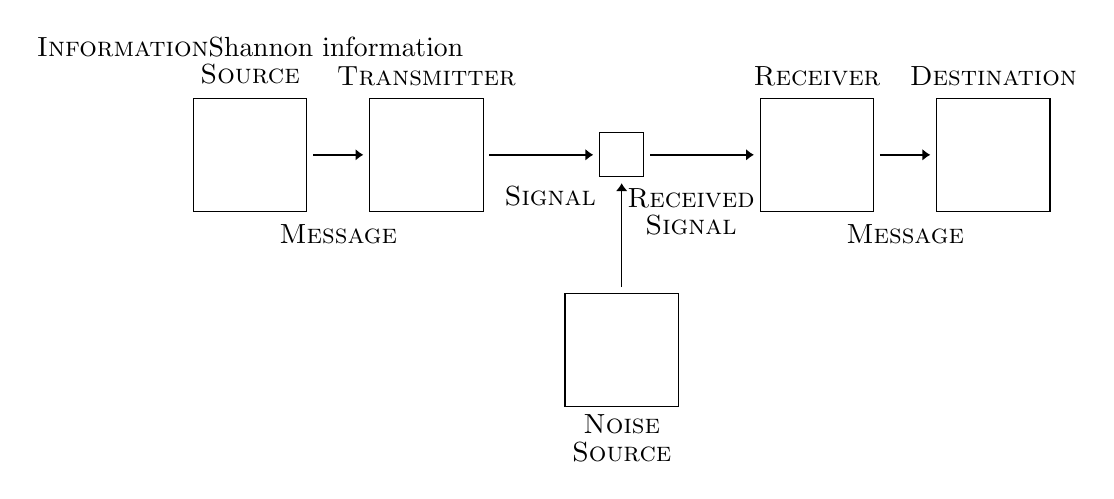
\begin{tikzpicture}[align=center, scale = .8]
 %%% Boxes
  \draw (0,0) rectangle (1.8,1.8);
  \draw (2.8,0) rectangle (4.6,1.8);
  \draw (6.45,.55) rectangle (7.15,1.25);
  \draw (9,0) rectangle (10.8,1.8);
  \draw (11.8,0) rectangle (13.6,1.8);
  \draw (5.9,-1.3) rectangle (7.7,-3.1);
%%% Arrows
 \draw [-{Latex[length=1mm,width=1.5mm]},line width=.2mm] (1.9,.9) -- (2.7,0.9);
 \draw [-{Latex[length=1mm,width=1.5mm]},line width=.2mm] (4.7,.9) -- (6.35,0.9);
 \draw [-{Latex[length=1mm,width=1.5mm]},line width=.2mm] (7.25,.9) -- (8.9,0.9);
 \draw [-{Latex[length=1mm,width=1.5mm]},line width=.2mm] (10.9,.9) -- (11.7,0.9);
 \draw [-{Latex[length=1mm,width=1.5mm]},line width=.2mm] (6.8, -1.2) -- (6.8,.45);

%%% Labels
 \node at (.9,2.4){\textsc{Information}\is{Shannon information}\\[-2pt]\textsc{Source}};
 \node at (3.7,2.15){\textsc{Transmitter}};
 \node at (9.9,2.15){\textsc{Receiver}};
 \node at (12.7,2.15){\textsc{Destination}};
 \node at (2.3,-0.35){\textsc{Message}};
 \node at (11.3,-0.35){\textsc{Message}};
 \node at (5.665,.25){\textsc{Signal}};
 \node at (7.9,.0){\textsc{Received}\\[-2pt]\textsc{Signal}};
 \node at (6.8,-3.6){\textsc{Noise}\\[-2pt]\textsc{Source}};
 \end{tikzpicture}
\caption{Shannon's model of communication \citep[381]{shannon1948}. \label{fig:shannon-cystem}}
\end{figure}

On an abstract level, encoding consists in assigning a signal to each possible message, and depending on which signal is assigned to which message, communication can be more or less efficient.  \citeauthor{shannon1948} distinguishes two properties of the channel that constrain the optimal form of signals to be sent through it, which must be considered by an encoding strategy in order to communicate efficiently.

\is{Noisy channel|(}First, the channel can be (and in practice most of the time is) noisy: Random noise can corrupt the signal during the transmission process, so that the signal passed to the recipient can differ from that sent by the source. For instance, if the signal consists in a sequence of letters A, B, and C, noise could transform a sent signal ABCA into ABBB. \citet[410]{shannon1948} observes that noise potentially constitutes a problem for communication, but that ``by sending the information\is{Shannon information} in a redundant form the probability of errors can be reduced.'' An example of redundant encoding is to send each letter four times. For the above signal, this yields AAAABBBBCCCCAAAA. If now only one of the four repetitions of each letter was corrupted by noise on average, the intended letter could still be recovered by assuming that the most frequent letter in each substring is the one intended by the sender. Of course, this encoding strategy makes communication less efficient: If the signal length is increased by the factor $n$, sending it will take $n$ times longer than sending the short signal. Therefore, efficient coding will involve a trade-off between the transmission of as much information\is{Shannon information} as possible in a given interval of time and minimizing the probability of errors by including additional redundancy. Second, the channel has a limited \textit{channel capacity}\is{Channel capacity}, which is measured in bits transmitted per unit of time. \citet[401--413]{shannon1948} shows that, given an appropriate coding system, information\is{Shannon information} can be transmitted with a very low error rate unless the transmission rate does not exceed channel capacity\is{Channel capacity}. However, when channel capacity\is{Channel capacity} is exceeded, the likelihood of errors increases faster than the gain in intended transmission rate. Hence, attempts of increasing the transmission rate above channel capacity\is{Channel capacity} will never yield an advantage, but further reduce the actual transmission rate.

Taken together, in order to communicate efficiently across a noisy channel\is{Noisy channel}, the best choice is to communicate at a rate close to but not exceeding channel capacity\is{Channel capacity}: Not making use of the available bandwidth would be inefficient and more time-consuming, while exceeding channel capacity\is{Channel capacity} harms the purpose of communication due to the increased likelihood of errors and, as \citeauthor{shannon1948} shows, will not yield an effectively higher transmission rate. In simplified terms, this requires interlocutors to allow for a certain degree of redundancy in their signal whenever channel capacity\is{Channel capacity} would be exceeded otherwise. As long as this is not the case, they should densify their utterance as much as possible in order to maximize efficiency.\is{Noisy channel|)}\is{Information theory|)}

On an abstract level, the idea that underlies information-theoretic\is{Information theory} research on language is that these general constraints on communication can explain optional variation in language. Grammar often provides a variety of signals that can be used to communicate a message, but does not explain why speakers choose a particular one in a specific situation. Specifically in the case of ellipsis, grammar determines whether an omission is licensed, but not all omissions that are licensed necessarily occur. From an information-theoretic\is{Information theory} perspective, a perfectly grammatical utterance might be dispreferred as compared to another one, for instance, because it is too redundant or because it exceeds channel capacity\is{Channel capacity}. This idea is worked out in detail in what follows.

\section{Information-theoretic constraints on language}
\label{sec:infotheory-language}

The model of communication in Figure \ref{fig:shannon-cystem} that \citet{shannon1948} assumes can easily be translated to any communicative situation between two interlocutors. Just like in the model, the speaker first has to  encode her message, which can be thought of as a proposition, into an acoustic or written signal. This signal is sent across an acoustic or visual channel to the hearer, who has to decode, i.e. parse\is{Parser, human} and interpret it. During the transmission process, the signal can be corrupted by noise\is{Noisy channel|(}. As I discuss in greater detail below, noise can be thought of as acoustic noise in the environment or as any other factor that results in a difference between the message sent by the speaker and the message received by the hearer.\is{Noisy channel|)} In principle, utterances can be optimized with respect to the properties of the communication system on any level of linguistic analysis, be it phonemes, morphemes, words, more abstract syntactic constructions or complete sentences.

The account of fragment usage that I propose assumes that interlocutors optimize their utterances with respect to the goal of communicating efficiently through a noisy channel\is{Noisy channel}, as has been shown by previous research on information-theoretic\is{Information theory} constraints on language. Applied to natural language, the encoding process consists in assigning a linguistic signal, i.e. an utterance, to the intended message, that is, the proposition to be communicated. In the case of the choice between fragment and sentential utterances this optimization can involve the optional omission of words in the utterance, which might result in a preference for the fragment.

\is{Source coding|(}\is{Channel coding|(}For the purpose of efficient communication, the encoding process must consider the properties of the components of the communication system. Previous research has identified two components of the model with respect to whose properties the signal is optimized: the source\is{Source coding} and the channel\is{Channel coding}. Most of the recent work on information theory\is{Information theory} in psycholinguistics, in particular studies on the UID\is{Uniform Information Density} hypothesis \citep{levy.jaeger2007}, focus on adaptation to properties of the channel. Even before that, \citet{zipf1935}\is{Zipf's Law} observed a relationship between the frequency and length of linguistic expressions which suggests that statistical properties of the source\is{Source coding} also constrain encoding preferences. As \citet{pate.goldwater2015} show, the optimization of the signal to properties of the source, which they term \textit{channel coding}\is{Channel coding} and \textit{source coding}\is{Source coding} make partially differing predictions. In order to specify testable predictions of information theory\is{Information theory} on the form and usage of fragments, effects of source and channel coding have to be teased apart. 

In what follows I discuss the predictions of source and channel coding on the form of utterances. It will become evident that both of these strategies predict that more frequent messages are more likely to be reduced, but only channel coding predicts the insertion of additional redundancy, the adaptation to the communicative situation and hence to the hearer's expectations.%
\footnote{My experiments do not investigate the adaptation to the communicative situation. For evidence with respect to this see e.g. \citet{pate.goldwater2015}.}\afterfn%
%
Furthermore, in the case of fragments, only channel coding\is{Channel coding} makes explicit predictions about \textit{which} words are omitted and which ones are realized. These are the predictions which I test in the two experiments in Chapter \ref{sec:chapter-infotheory-experiments}.\is{Source coding|)}\is{Channel coding|)}

\subsection{Source coding}
\label{sec:infotheory-zipf}
\is{Source coding|(}

In \citepos{shannon1948} terminology, the source is the part of the communication system that generates messages, which then have to be encoded in order to be sent over the channel. Source coding\is{Source coding} focuses on the probability distribution over possible messages. In applications of information theory\is{Information theory} to linguistic phenomena the possible messages will differ in their likelihood most of the time. For instance, in a pub scenario, it is relatively likely that the customer will order drinks and food (in particular specific types thereof), but less likely that he wants to tell the waiter about an interesting linguistic paper that he recently read.\is{Context, extralinguistic} As I discussed in Section \ref{sec:infotheory-noisy-channel}, encoding consists in assigning a signal to each message, and most of the time the expressions that are available in the set of possible signals differ in length. In this situation, an efficient source coding strategy reserves the shorter signals for likely messages and assigns longer signals to unlikely ones \citep[402]{shannon1948}. This reduces the average length of an actually produced signal on average, because it ensures that shorter signals are sent more often.

\is{Zipf's Law|(}
Source coding\is{Source coding} effects have been reported specifically on the word level, since \citet{zipf1935}\is{Zipf's Law} observed that more frequent words tend to be shorter on average in English\il{English}, Latin and Chinese\il{Chinese}.%
%
\footnote{\citeauthor{zipf1935} himself refers to \citet{kaeding1897} and \citet{eldridge1911} for previous tentative evidence in favor of this hypothesis. \citet[23--25]{zipf1935} however argues that for methodological reasons neither of these studies ultimately confirms the hypothesis.}\afterfn%
%
This motivates his Law of Abbreviation, which states that ``as the relative frequency of a word increases, it tends to diminish in magnitude.'' He argues that this principle results from a tendency toward ``saving of time and effort'' \citep[38]{zipf1935}. The number of possible short words in a language is naturally restricted by the limited inventory of phonemes and the syllabic structure of that language. Assigning shorter signals to more frequent messages reduces the average length of a random word as compared to a hypothetical language where there is no correlation between frequency and length. Consequently, the length-frequency correlation allows for the transmission of more words in less time, or, in the case of written speech, space.%
%
\footnote{\citet[30--36]{zipf1935} relates diachronic changes, like the shortening of \textit{gasoline} to \textit{gas} and the substitution of \textit{automobile} by \textit{car}, to an adaption to the increased frequency of these words.}\afterfn%
%
More recently, \citepos{zipf1935} observation has been replicated for a larger sample of languages by \citet{piantadosi.etal2011} and for semantically similar words that differ in length (e.g. \textit{math} vs. \textit{mathematics}) by \citet{mahowald.etal2013}.%
%
\footnote{\citet{mahowald.etal2018} furthermore show that across a variety of languages, even when word length is controlled, more frequent words have more phonotactically probable forms than less frequent ones.}\afterfn%
%
\is{Zipf's Law|)}

The idea that shorter signals are assigned to more frequent, i.e. likely, messages can be extended to the sentence level. Source coding\is{Source coding} then predicts that more frequent messages are preferably encoded as a fragment. Unlikely messages will rather be encoded as a full sentence if all of the shorter fragments have already been allocated to more likely messages. \is{Context, extralinguistic|(}For instance, consider an extremely simplified taxi scenario, which models the communicative situation after a pedestrian (the speaker) hailed a taxi. In the scenario, there are only two messages that differ in their probability \Next%
%
\footnote{For expository purposes, I do not provide semantic representations in this case, but simply a paraphrase of the speaker's communicative intention.}\afterfn%
% 
and three signals that differ in length \NNext, including a fragment \NNext[c]. Since the fragment can be derived from both \NNext[a] and \NNext[b], it can encode both messages in \Next. A speaker who performs source coding\is{Source coding} will assign the fragment to the more probable message \Next[a], so that the only way of encoding the less informative\is{Shannon information} message in \Next[b] is the less informative\is{Shannon information} full sentence in \Next[b].\is{Context, extralinguistic|)}

\ex. Messages
\a. The pedestrian wants a ride to the university.\hfill $p = a;\;a > 0.5$
     \b. The pedestrian wants to know how to get to the university. \hfill$p = 1-a$

\ex. Signals
\a. Take me to the university, please! \hfill $length = 6$
     \b. Explain me the way to the university, please! \hfill $length = 8$
     \c. To the university, please!\hfill $length = 4$

Source coding\is{Source coding} consequently predicts that more likely messages are more often encoded as fragments, but this does not necessarily imply that less likely messages are preferably encoded as full sentences: In a hypothetical situation with very few possible messages, as long as there is a sufficient number of fragments to encode all messages, none of the messages will be encoded as a sentence. Source coding\is{Source coding} thus predicts no upper bound on densification: If unpredictable messages receive longer signals, this is only a by-product of the assignment of short signals to predictable messages, as the taxi example illustrated.\is{Source coding|)}

Source coding\is{Source coding} on the sentence level also makes no predictions on the internal form of the signal. It can explain why fragments are more often used to communicate predictable messages, but it cannot explain why specific words are omitted in these fragments. As will become evident throughout the next section, this is predicted only by channel coding\is{Channel coding} accounts like Uniform Information Density\is{Uniform Information Density}.

\subsection{Channel coding}
\label{sec:infotheory-uid}
Focusing on the source alone disregards the idea that the signal is transmitted over a noisy channel\is{Noisy channel} with limited capacity\is{Channel capacity} in \citeauthor{shannon1948}'s model: Speakers should not only optimize their utterance with respect to properties of the source\is{Source coding}, but also with respect to those of the channel. In particular, they should avoid exceeding or repeatedly underutilizing the available capacity\is{Channel capacity}. This requires them to keep track of the distribution of information\is{Shannon information} across the signal. Channel coding\is{Channel coding} predicts a preference for those signals that ensure a transmission rate below but close to channel capacity\is{Channel capacity}. This is the main difference between the prediction between source and channel coding, because source coding\is{Source coding} imposes no such upper bound on the densification of the signal.

\subsubsection{Uniform Information Density}
\is{Channel coding|(}
In the literature, channel coding\is{Channel coding} has been discussed under different labels. In what follows, I sketch the general idea, its psychological reality and methods used to investigate its empirically testable predictions.

The idea that speakers adapt their utterance to the channel has been applied to linguistic phenomena for the first time by \citet{fenk.fenk1980}, \citet{fenk-oczlon1989} and \citet{fenk-oczlon1990} even before the more recent rise of information-theoretic\is{Information theory} accounts of language processing in psycholinguistics. \citet{fenk.fenk1980} proposed a principle of \textit{Constant Flow of Information}\is{Shannon information}, which states that the amount of information sent by unit of time\is{Information density} varies only weakly around a constant mean \citep[38]{fenk-oczlon1990}. \citet[403]{fenk.fenk1980} argue that increasing the rate of transmission too far above this mean would exceed the processing capacity\is{Processing effort} of the hearer, whereas falling below the mean would be inefficient. This approach models channel capacity\is{Channel capacity} as an upper bound on the cognitive resources\is{Processing effort} of the hearer, an idea that I also adopt in this book (see Section \ref{sec:infotheory-effort} for details).

\is{Uniform Information Density|(}
More recently, the idea that speakers tend toward distributing information\is{Shannon information} uniformly across the speech signal has been reformulated for different levels of linguistic analysis. For instance, the \textit{Smooth Signal Redundancy} hypothesis by \citet{aylett.turk2004} predicts that speech is smoothed on the phonetic level by modulating the length of syllables. On the level of complete sentences, \citet{genzel.charniak2002, genzel.charniak2003} propose an \textit{Entropy\is{Entropy} Rate Constancy} principle, which states that the average entropy\is{Entropy} of sentences throughout a text is constant. Whereas these principles are related to specific levels of analysis, \citet[24]{levy.jaeger2007} explicitly claim that their \textit{Uniform Information Density}\is{Uniform Information Density} (UID) hypothesis holds on any level of analysis. Work relying on the notion of UID has mostly focused on morphosyntactic variation, such as contractions \citep{frank.jaeger2008} and omissions of function words \citep{levy.jaeger2007, jaeger2010} as well as grammatical markers \citep{kurumada.jaeger2015, norcliffe.jaeger2016}, which will turn out to be particularly relevant to the investigation of omissions in fragments. For this reason, I will use the notion of UID in order to refer to the principle of distributing Shannon information\is{Shannon information} as uniformly as possible across the utterance.

On an abstract level, UID\is{Uniform Information Density} predicts that if there are several signals that can encode a message, everything else being equal, the speaker will choose the signal which comes closest to the ideal distribution of information\is{Shannon information}\is{Information density}, which approximates channel capacity\is{Channel capacity} without exceeding it. At least in the original version of the theory, the set of possible signals is restricted to grammatical expressions, since \citet[25]{jaeger2010} argues that optional variation occurs only within ``the bounds defined by grammar.'' This assumption is crucial to the empirical investigation of fragments, because it implies that UID\is{Uniform Information Density} favors the most well-formed \textit{grammatical} signal and does not take into account utterances that might distribute information\is{Shannon information} even more uniformly but that cannot be derived by grammar.

Following \citet[849]{levy.jaeger2007}, the \textit{information\is{Shannon information} density\is{Information density}} of an utterance is defined as ``the amount of information\is{Shannon information} per unit comprising the utterance'', that is, the sum of the information\is{Shannon information} carried by each individual word within the utterance. This total information\is{Shannon information} density\is{Information density} mass is to be distributed as uniformly as possible across the words comprising the utterance. Distributing information\is{Shannon information} uniformly implies that speakers ``avoid peaks and troughs in information\is{Shannon information} density\is{Information density}'' \citep[849]{levy.jaeger2007}, which result from transmitting too little or too much information\is{Shannon information} per unit of time. In that sense, troughs are local information\is{Shannon information} minima that result in an inefficient use of channel capacity\is{Channel capacity}, whereas peaks are information maxima that exceed channel capacity\is{Channel capacity} and therefore hamper communication. %
\is{Channel coding|)}
\is{Uniform Information Density|)}

\subsubsection{UID effects on omissions}
In order to illustrate how omissions in fragments may contribute to the optimization of utterances with respect to UID\is{Uniform Information Density}, consider again the taxi example that I discussed above. In this situation, a pedestrian hails a taxi, because he needs a ride to the university. In this simplified example, he can in principle choose between a full sentence \Next[a] and a fragment \Next[b] to communicate this message.%
%
\footnote{Of course, this is highly simplified, because he could make use of a wide variety of different syntactic constructions and lexicalizations of fragments and sentences.}\afterfn%
% 

\ex. \label{ex:uid-taxi}
\a. Take me to the university, please.
     \b. To the university, please.

In the taxi scenario it will be in general very likely\is{Context, extralinguistic} that the passenger wants to go somewhere, so the material that is omitted in the fragment (\textit{take me}) is very predictable. In contrast, it is unlikely that the driver knows the passenger's destination, this destination is unpredictable and relatively informative. Figure \ref{fig:fragments-uid-predictable}, which shows the distribution of information\is{Shannon information} over time,%
%
\footnote{The variable on the abscissa in principle is time, because channel capacity\is{Channel capacity} and transmission rates are defined as an amount of information\is{Shannon information} transmitted per unit of time, e.g. in bits per second. In practice, however, specifically corpus\is{Corpus}-based work \citep[see e.g.][]{levy.jaeger2007, frank.jaeger2008, jaeger2010} simplifies this to the amount of information\is{Shannon information} transmitted per word, because duration measures for words or appropriate transcriptions into phonemes are not available in the corpora\is{Corpus} or would complicate the statistical analysis.}\afterfn%
%
illustrates this idea with hypothetical information density\is{Information density} (ID) profiles for the fragment and the corresponding full sentence. 

\begin{figure}[t]
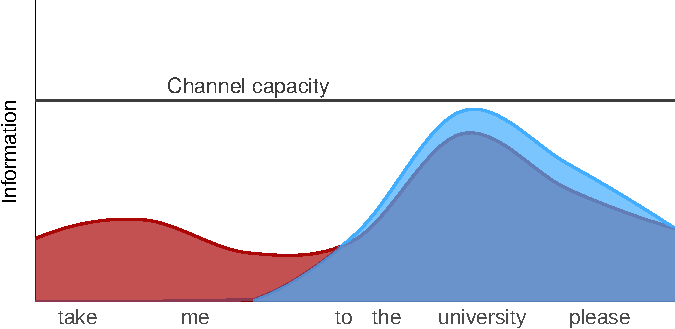
\includegraphics[scale=1]{figures/uid-example-fragment}
 \caption{Hypothetical ID profile for the predictable sentence \textit{take me to the university} and the meaning-equivalent fragment \textit{to the university} in the taxi scenario. The blue area illustrates the distribution of information in the fragment and the red area that in the full sentence.\label{fig:fragments-uid-predictable}}
\end{figure}

\is{Context, extralinguistic|(}If the pedestrian wants the driver to tell him the way to the university instead, he has to choose between the fragment in \Last[b] and the sentence in \Next. In that case, \textit{tell me the way} is probably less predictable than \textit{take me}, as Figure \ref{fig:fragments-uid-unpredictable} suggests. Of course, whether a word is predictable depends on properties of the utterance context. For instance, when an utterance like \Next is not produced by a passenger approaching the taxi, but by the driver of another car with a foreign license plate, it might be more likely that he would ask the local taxi driver for the way than that he wants to go somewhere. Similarly, when the passenger is brought to the university by the same driver on every Wednesday, or he wears a Denver Nuggets hat and shirt an hour before the match starts, the destination might be more likely and the utterance possibly even further reduced.\is{Context, extralinguistic|)} %

\ex. Tell me the way to the university, please.

\begin{figure}[t]
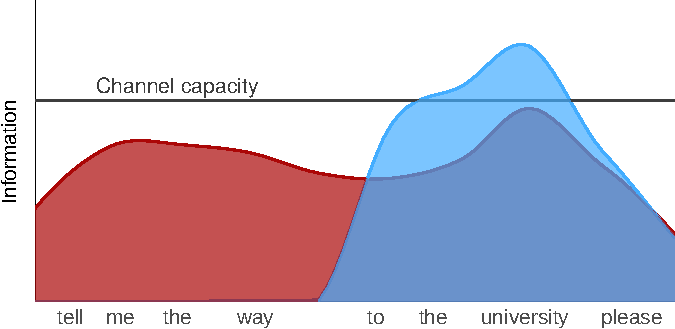
\includegraphics[scale=1]{figures/uid-example-sentence}
\caption{Hypothetical ID profile for the unpredictable sentence \textit{tell me the way to the university} and the meaning-equivalent fragment \textit{to the university} in the taxi scenario. The blue area illustrates the distribution of information in the fragment and the red area that in the full sentence.\label{fig:fragments-uid-unpredictable}}
\end{figure}
%
Figure \ref{fig:fragments-uid-predictable} shows how the local information\is{Shannon information} minimum, or \textit{trough}, in the ID profile\is{Information density} that is caused by the redundant \textit{take me} is smoothed by omitting this expression. From a UID\is{Uniform Information Density} perspective, omitting such predictable words optimizes the signal. If these omissions target words that are obligatory in full sentences, this results in the preference of the fragment over the full sentence. In contrast, given the density\is{Information density} profiles in \ref{fig:fragments-uid-unpredictable}, \textit{tell me the way} does not yield a trough in the profile, hence there is no pressure to omit these words. Furthermore, its omission would result in a \textit{peak} in the density\is{Information density} profile that exceeds channel capacity\is{Channel capacity}.%
%
\footnote{Note that Figure \ref{fig:fragments-uid-unpredictable} is not fully accurate, because I assigned the identical fragment \textit{to the university} different density\is{Information density} profiles in the left and right panel for the purpose of illustration. See below in this section for a discussion of this issue.}\afterfn%
%
Therefore, from the UID\is{Uniform Information Density} perspective, it is not beneficial to omit these words. Actually, even if \textit{tell me} was redundant, its insertion is preferred as long as it contributes to reducing the peak on \textit{to the university}. 

The tendencies to (i) to omit predictable expressions and (ii) to realize expressions that reduce peaks on upcoming material are the central predictions of UID\is{Uniform Information Density} on the well-formedness of linguistic expressions. Both of them are empirically supported by previous research, as \citet{frank.jaeger2008} show for contraction in English\il{English}, \citet{kurumada.jaeger2015} for Japanese case markers, \citet{levy.jaeger2007} for relative pronouns in English\il{English}, \citet{jaeger2010} for complementizers, \citet{norcliffe.jaeger2016} for relative pronouns in Yucatec Maya, \citet{asr.demberg2015} for discourse markers and \citet{lemke.etal2017} for articles\is{Article omission}. With the exception of \citet{kravtchenko2014}, who investigates the omission of subjects in Russian\il{Russian}\is{Subject drop}, these studies investigate semantically relatively vacuous function words. It is therefore reasonable to assume that UID\is{Uniform Information Density} constrains omissions in fragments too, but this does not necessarily follow from previous research. The finding by \citet{tily.piantadosi2009} that more predictable nouns are more likely to be pronominalized, i.e. reduced, points in a similar direction, if ellipsis as a more radical form of reduction of given material. Furthermore, the relationship between predictability and reduction has also been evidenced by studies which find that predictable expressions are more likely to be reduced in terms of duration and/or articulatory effort both on the word level and on that of individual syllables \citep[see e.g.][]{bell.etal2003, aylett.turk2004,  bell.etal2009, tily.etal2009, demberg.etal2012, kuperman.bresnan2012, seyfarth2014, pate.goldwater2015, brandt.etal2017, brandt.etal2018,  malisz.etal2018}.

Even though the concept is labeled \textit{Uniform} Information Density, at least in the version adopted in current psycholinguistics, the property of uniformity is an artifact of the assumptions made and not a goal of the encoding strategy in its own right. Uniformity only follows from the approximation of the transmission rate to the channel capacity\is{Channel capacity}, but a uniform distribution far below channel capacity\is{Channel capacity} will still be dispreferred compared to less uniform signals that make a more efficient use of channel capacity\is{Channel capacity}. This leads to an important distinction between the effect of peaks and troughs with respect to the choice between alternative ways of encoding a message. Troughs are inefficient and therefore always to be avoided, if possible. In contrast, peaks only dispreferred if they exceed channel capacity\is{Channel capacity}. In what follows, I will imply this interpretation of uniformity when stating that a signal is more or less compliant to UID\is{Uniform Information Density}, unless stated otherwise.

As for now, there have been no attempts to quantify channel capacity\is{Channel capacity}. This would not be a promising endeavor, because, as \citet{shannon1948} showed, channel capacity\is{Channel capacity} is not a constant, but varies as a function of the noise rate\is{Noisy channel} in the channel. This indeterminacy of channel capacity\is{Channel capacity} is expected if UID\is{Uniform Information Density} is interpreted as a psycholinguistic constraint on communication. UID\is{Uniform Information Density} implies that speakers are engaged in audience design\is{Audience design} and adapt their utterances to expected properties (e.g. preferences and cognitive abilities) of the hearer, so this will necessarily involve inferences under uncertainty about channel capacity\is{Channel capacity}. Furthermore, from a methodological perspective, the absolute information\is{Shannon information} estimate depends on the corpus\is{Corpus} used for this purpose. Since information\is{Shannon information} is based on probabilities, a larger lexicon will result in lower average probabilities of individual items. What matters for empirical research on UID\is{Uniform Information Density} is that, even if channel capacity\is{Channel capacity} is unknown, on average, more informative\is{Shannon information} words are more likely to yield a peak and more uninformative words are more likely to cause a trough in the ID profile\is{Information density}.

Taken together, UID\is{Uniform Information Density} predicts that, given a set of possible signals, i.e. sentential and nonsentential utterances that can be used to encode a message and that comply with grammar,%
%
\footnote{Most of the time, this set of possible signals will be too large to empirically evaluate the alternatives. Even if no fragments were considered at all, a theoretically infinite number of sentences can be used to convey a single message. Therefore, when it comes to evaluating the alternative set empirically, I will assume that there is one sentence equivalent to each message from which a set of fragment alternatives is derived by ellipsis. This concerns in particular the evaluation of the production study\is{Production task} in Section \ref{sec:scripts-production}.}\afterfn%
% 
the preferred utterance is that which distributes information\is{Shannon information} most uniformly across the utterance. This leads to the two specific predictions in \Next[a,b], which in turn imply \Next[c]: If omissions occur more often in predictive contexts, because average words are more likely, the signal will on average be shorter in such situations.

\ex. \textit{Predictions of UID\is{Uniform Information Density} on fragments} \label{ex:uid-fragments-predictions}
\a. \textit{Avoid troughs}: The more likely a word is in context, the more likely it is to be omitted (within the limits of grammar).\label{ex:uid-fragments-predictions-troughs}
 \b. \textit{Avoid peaks}: Uninformative words can be inserted before very informative words in order to lower the surprisal\is{Shannon information} of the latter (within the limits of grammar).\label{ex:uid-fragments-predictions-peaks}
 \c. \textit{Densification}: Shorter signals, like fragments, are preferred in predictive contexts.\label{ex:uid-fragments-predictions-densification}

\subsubsection{UID effects on word order}
\is{Word order|(}
The distribution of information\is{Shannon information} across the signal can also be optimized by reordering the expressions that it comprises. Effects of word order\is{Word order} on UID\is{Uniform Information Density} are not as central to my research question as omissions, because they are not unique to fragments, but my experiment \ref{exp:scripts-production} will also show that there is evidence for UID\is{Uniform Information Density} effects on word order\is{Word order}. \is{Context, linguistic|(}Word order\is{Word order} effects are predicted by UID\is{Uniform Information Density} because a word's information depends on the context in which it occurs and variation of word order changes this context. In general, the larger the context of a word is, the more predictable this word tends to become, because preceding material narrows the range of possible continuations of the utterance. This has also been shown by \citet{levy2008} for verb-final contexts in German\il{German} based on reading time data by \citet{konieczny.doring2003}. The more arguments of the final verb the hearer parses\is{Parser, human}, the smaller does the set of potential completions of the sentence become. This surprisal\is{Shannon information} reduction is reflected in reduced reading times for words that occur later in the clause. \citet{fenk-oczlon1983} argues that this also accounts for the general tendency for given or topicalized expressions to precede new or focused ones \citep{chafe1976}: Given expressions are on average more predictable than new ones, and therefore this ordering reduces the information of the new ones and yields a more uniform ID profile\is{Information density}.\is{Context, linguistic|)}%
%
\footnote{Most of the time, topicality and high predictability will probably cooccur. However, these concepts operate on different levels of analysis. Topicality determines what an utterance is about \citep{reinhart1981, krifka2007} but predictability determines only the likelihood of a word to be mentioned at a particular point within the utterance. Expressions can be predictable, but not topical, if they have are likely in context and they are focused. For instance, in \Next, taken from \citet{kuperberg.etal2020}, the target noun \textit{swimmers} has a high cloze probability as compared to \textit{trainees} or \textit{drawer} -- all of these three words appear in the comment and the topic of the sentence are the lifeguards.

\ex. The lifeguards received a report of sharks right near the beach. Their immediate concern was to prevent any incidents in the sea. Hence, they cautioned the (swimmers/trainees/drawer).

}\afterfn%
% 
More recently, \citet{sikos.etal2017} report an effect of UID\is{Uniform Information Density} on the choice between pre- and postnominal modification of German\il{German} nouns, and \citet{speyer.lemke2017} observe an effect of the aggregated surprisal\is{Shannon information} of relative clauses on their extraposition in historic stages of German\il{German}.

Even though UID\is{Uniform Information Density} predicts effects on word order\is{Word order}, fragments often do not allow for word order\is{Word order} variation. For instance, in a German\il{German} DP\is{Determiner phrase} or PP\is{Preposition phrase}, word order\is{Word order} is relatively fixed and determined by grammar, and UID\is{Uniform Information Density} only determines the choice between grammatical expressions. I return to this issue in the discussion of experiment \ref{exp:scripts-production}, because the data set that I collected in this study is suitable for the investigation of UID\is{Uniform Information Density} effects on optional word order\is{Word order} variation, too.%
%
\footnote{Exceptions to the fixed word order within DPs and PPs are e.g. DPs\is{Determiner phrase} that contain multiple adjectives \Next and a few prepositions that can also appear postnominally \NNext. I leave such variation aside, because in the first case there are semantic and phonological constraints that strongly bias the ordering of adjectives \citep{martin1969, dixon1977, cinque1994, wulff2003}, and postposition \NNext is restricted to single lexical items \citep{dimeola2003}.

\ex. \ag. das neue schnelle Fahrrad\\
	  the new fast bike\\
     \bg. das schnelle neue Fahrrad\\
	  the fast new bike\\
	  \trans{the fast new bike}

\ex. \ag. wegen des Regens\\
	  because the.\textsc{gen} rain.\textsc{gen}\\
      \bg. des Regens wegen\\
	  the.\textsc{gen} rain.\textsc{gen} because\\
	  \trans{because of the rain}

}\afterfn%
%
\is{Word order|)}

\subsubsection{Summary: Predictions of UID on the form of fragments}
UID\is{Uniform Information Density} makes empirically testable predictions with respect to the preferred way of encoding of a message. Speakers use omissions of optional words in order to modulate the information density profile\is{Information density} in two ways: On the one hand, omitting uninformative words can smooth the profile by avoiding troughs. On the other hand, the insertion of redundant words before otherwise unpredictable ones reduces peaks in the profile. Such effects, which will be observed on the word level, are more specific than the general preference to assign shorter utterances to more predictable messages that follows from source coding\is{Source coding}. This relationship between the probability of a message and the length of the signal that source coding\is{Source coding} predicts also results from UID\is{Uniform Information Density}. For predictable messages, the individual words will also be on average more likely, so that there will be a higher ratio of omissions, which in turn results in a shorter signal. While UID\is{Uniform Information Density} and source coding\is{Source coding} share the prediction that shorter signals are assigned to more likely messages, only UID\is{Uniform Information Density} predicts \textit{which} words are omitted in fragments.

\subsection{UID as efficient distribution of processing effort} 
\label{sec:infotheory-effort}
The studies cited above support the basic prediction of UID\is{Uniform Information Density}, that is, the tendency of distributing information\is{Shannon information} uniformly across the utterance. However, in the literature two different ways of mapping the abstract concepts in \citeauthor{shannon1948}'s model of communication to natural language have been suggested. These interpretations differ particularly with respect to the channel. On the one hand, specifically in phonetic research, the channel is interpreted rather literally as the space through which the signal is sent \citep[see e.g.][]{aylett.turk2004}. On the other hand, from a psycholinguistic perspective, the channel has been related to the processing resources\is{Processing effort} available to the hearer, and channel capacity\is{Channel capacity} interpreted as an upper bound to these resources \citep[see e.g.][]{fenk.fenk1980}. Before returning to UID\is{Uniform Information Density} effects on omissions, I briefly review these approaches and argue why I adopt the second possibility and interpret Shannon information\is{Shannon information} as a measure of processing effort, as has been suggested e.g. by \citet{hale2001} and \citet{levy2008}. 

\is{Noisy channel|(}The interpretation of the channel which is more closely related to the communicative situation modeled by \citet{shannon1948} conceptualizes the channel as the medium between speaker and hearer. From this perspective, the message can be corrupted by noise\is{Noisy channel} during transmission and UID\is{Uniform Information Density} ensures ``robust information\is{Shannon information} transfer in a potentially noisy environment while conserving effort'', as \citet[32]{aylett.turk2004} put it. Noise can be acoustic, but it can also consist in other modifications of the signal, like hearers being distracted by other tasks \citep{hauser.etal2019}. As \citet{shannon1948} showed, an increased likelihood of noise reduces channel capacity\is{Channel capacity}, because the potential corruption of the message has to be counterbalanced by inserting additional redundancy. In particular on the phonetic level and in case of high noise ratios this is a reasonable assumption, because the prediction of information\is{Shannon information} theory\is{Information theory} that speakers adapt their utterances in the presence of acoustic noise is a well-established finding, known as the \textit{Lombard effect}  \citep{lombard1911}. Experimental research has shown that this adaptation concerns a variety of parameters, including an increase in F0, speech level and vowel duration \citep{summers.etal1988,junqua1994, junqua1996}. This is in line with information\is{Shannon information}-theoretic studies that find effects of predictability on the articulation and duration of words and phonemes \citep{bell.etal2003, aylett.turk2004, bell.etal2009, brandt.etal2017, brandt.etal2018, malisz.etal2018}.\is{Noisy channel|)}

However, it is unclear whether the assumption that UID\is{Uniform Information Density} effects are related to the presence of environmental noise holds to the same extent for higher levels of linguistic analysis, such as words or complete sentences. In regular face-to-face communication, in the absence of a significant source of acoustic noise, and specifically if the word level is concerned, it seems relatively unlikely that complete are misheard. Words that are similar to each other, like \textit{Harry} and \textit{Mary} might be misunderstood if a part of the word is corrupted by noise, but it is less likely that \textit{Harry} is misunderstood as \textit{Susan} for this reason.

\is{Processing effort|(}The link between predictability and processing effort\is{Processing effort} allows for an interpretation of UID\is{Uniform Information Density} as a strategy to communicate efficiently even in the absence of (perceptual) noise. \citet[850]{levy.jaeger2007} note that ``independently of whether linguistic communication is viewed as a noisy channel\is{Noisy channel}, UID\is{Uniform Information Density} can be seen as minimizing comprehension difficulty.'' This is based on the insight that the effort\is{Processing effort} required to process an expression is proportional to its predictability in context \citep{hale2001, hale2016, levy2005, levy2008}. In psycholinguistics it is a well-established finding that, everything else being equal, more predictable words are read faster \citep[see e.g.][]{ehrlich.rayner1981, mcdonald.shillcock2003, demberg.keller2008, smith.levy2013}. \citet[850]{levy.jaeger2007} relate UID\is{Uniform Information Density} and processing effort\is{Processing effort} by suggesting that a uniform distribution of information\is{Shannon information} minimizes the total processing effort\is{Processing effort} of an utterance, which they define as the sum of the processing effort\is{Processing effort} of all the words within this utterance.%
%
\footnote{There is some disagreement in the literature on the scale on which processing effort\is{Processing effort} and word probability are related. \citet{levy.jaeger2007} note that this conclusion presupposes that the relationship between surprisal\is{Shannon information} and processing effort\is{Processing effort} is superlinear, but this assumption has been questioned more recently. For instance, \citet{smith.levy2008, smith.levy2013} conclude that the relationship between surprisal\is{Shannon information} and processing effort\is{Processing effort} (as quantified by reading times in eye tracking\is{Eye tracking} and self-paced reading experiments) is linear, and more recently, \citet{brothers.kuperberg2019} argue that raw corpus\is{Corpus} frequency is a better predictor of reading times than surprisal\is{Shannon information}. Despite these concerns, even \citet[311]{smith.levy2013}, who argue against the superlinear relation, note that, if surprisal\is{Shannon information} indexes processing effort\is{Processing effort}, speakers should not overload their interlocutors' working memory. Similarly, \citet[51]{jaeger2010} argues that this relationship ``might be expected from any system that has access to limited resources.''
}\afterfn%
%
From this perspective, the concept of channel capacity\is{Channel capacity} in \citeauthor{shannon1948}'s model can be interpreted as delimiting the upper bound of the processing resources\is{Processing effort} available to the hearer for language comprehension within a given amount of time.%
%
\footnote{This predicts effects of the situational context on channel capacity\is{Channel capacity} even in the absence of strong noise sources. For instance, if competing tasks that require a share of the cognitive resources\is{Processing effort} which are otherwise available for language processing, this will also reduce channel capacity\is{Channel capacity} \citep{engonopoulos.etal2013,hauser.etal2019}. The prediction of UID\is{Uniform Information Density} is that if speakers are aware of that the hearer's resources are allocated otherwise, they will also reduce the information density\is{Information density} of their utterance by making their utterance more redundant.}\afterfn%
%
I follow this reasoning and therefore interpret channel capacity\is{Channel capacity} as an unknown and variable upper bound to the cognitive resources\is{Processing effort} that are available to the hearer for processing within a fixed interval of time. Therefore, the results of the experiments on fragment usage presented below do not hinge on a specific (linear or logarithmic) relationship between the likelihood of a word and the effort required for processing it, but on the assumption that the cognitive resources\is{Processing effort} available to the hearer are limited and on the insight that predictable words require less processing effort\is{Processing effort}.\is{Processing effort|)}

But \textit{why} would processing effort\is{Processing effort} be correlated to the probability of words or constructions in the first place? Following \citet{hale2001} and subsequent work \citep{levy2005, hale2006, levy2008}, the central idea is that processing effort\is{Processing effort} is proportional to the work done by the human parser\is{Parser, human}. Under the assumption of a fully parallel parser\is{Parser, parallel}\is{Parser, human}, this work consists in discarding those parses\is{Parser, parallel} that are incompatible with an input.%
%
\footnote{In contrast to \citet{hale2001}, \citet{levy2008} uses Kullback-Leibler divergence between probability distributions over parses\is{Parser, parallel} before and after processing an input. \citeauthor{levy2008}'s approach is also sensitive to gradual changes in probability that do not result in the rejection of a parse.}\afterfn%
%
In \citepos{hale2001} model, the information\is{Shannon information}, and consequently the processing effort\is{Processing effort}, of a word is higher, the larger the cumulated probability mass of the parses\is{Parser, parallel} that it disconfirms is. Formally, \citet[162]{hale2001} derives the surprisal\is{Shannon information} of a word as shown in Equation \ref{eq:surprisalhale}, where the prefix probability $\alpha_n$ is the cumulated probability mass of all parses\is{Parser, parallel} that are compatible with the input at the corresponding word and $\alpha_{n-1}$ is the cumulated probability mass of the parses\is{Parser, parallel} compatible with the previous word.

\begin{equation}
 \displaystyle S(w_n) = \log_2 \frac{\alpha_{n-1}}{\alpha_n} \label{eq:surprisalhale}
\end{equation}

This measure is equivalent to \citepos{shannon1948} definition of information\is{Shannon information}, because the higher the probability mass of the parses\is{Parser, parallel} that are compatible with a word is, the more predictable this word is. Since all $\alpha\leq1$ and $\alpha_n\leq\alpha_{n-1}$, the larger the probability mass of the parses\is{Parser, parallel} that are compatible with $w_{n-1}$ but not $w_n$ is, the higher is the surprisal\is{Shannon information} of $w_n$. Surprisal\is{Shannon information} equals 0 in case $w_n$ excludes no parse that is compatible with $w_{n-1}$.

Taken together, there are two ways of interpreting the channel with respect to natural language: one based on the presence of noise in the channel and one relating Shannon information\is{Shannon information} and processing effort\is{Processing effort}. It is beyond the scope of this work to test whether the noisy channel\is{Noisy channel}-based or the processing-based interpretation of UID\is{Uniform Information Density} is correct, and they are not mutually exclusive. However, the processing effort\is{Processing effort} version of UID\is{Uniform Information Density} seems intuitively more plausible to account for omissions in fragments.

\subsection{UID vs. other accounts of predictability-driven reduction}
\label{sec:infotheory-uid-competing}
In the introduction to this chapter, I noted that currently there is no comprehensive theory of why specific omissions in fragments occur. However, there are two potential alternative explanations for part of the predictability effects on omissions in fragments that UID\is{Uniform Information Density} predicts. First, \citet{ferreira.dell2000} analyze the optional omission of function words as driven solely by properties of language production. Second, information-theoretic\is{Information theory} measures like surprisal\is{Shannon information} are probably often correlated to information-structural\is{Information structure} concepts like givenness, focus or topicality. Therefore, I dedicate the remainder of this chapter to distinguishing the predictions of these approaches from the information-theoretic\is{Information theory} one that I pursue. 

\subsubsection{Availability-based production}
\label{sec:infotheory-uid-competing-abp}\largerpage

\is{Availability-based production|(}
Availability-based production\is{Availability-based production} \citep[e.g.][]{bock1987, ferreira.dell2000} explains part of the data that I interpreted above as evidence for UID\is{Uniform Information Density} as the result of properties of language production.%
%
\footnote{See also \citet{jaeger.buz2017} for an overview and a comparison to UID\is{Uniform Information Density}.}\afterfn%
% 
This approach relies on the difficulty of retrieving a lemma from memory. The idea is that speakers intend to produce speech fluently, and that the effortful retrieval of infrequent words delays speech production and thus results in disfluencies. These disfluencies are counterbalanced by inserting optional words that keep speech production fluent. As \citet[299]{ferreira.dell2000} suggest, the insertion of such words has a similar effect as an ``um''.

The main prediction of this approach is that insertions of optional words occur before unpredictable words, as \citet{ferreira.dell2000} show for complementizers in English\il{English}. UID\is{Uniform Information Density} predicts this too, but for a different reason: Realizing words before unpredictable ones can reduce the surprisal\is{Shannon information} of the latter and hence smooth peaks in the ID profile\is{Information density}. However, availability-based production\is{Availability-based production} neither implies that words that are themselves more predictable are more likely to be reduced, nor that predictable words tend to appear toward the beginning of the sentence. Therefore, if they were empirically confirmed, these two predictions will provide evidence for UID\is{Uniform Information Density}. Since UID\is{Uniform Information Density} and availability-based production\is{Availability-based production} are theories about different aspects of language, as \citet{jaeger.buz2017} note, they do not mutually exclude each other, but what matters in the context of my experiments is that data that cannot be explained by production preferences alone will support UID\is{Uniform Information Density}.\is{Availability-based production|)}

\subsubsection{Information structure}\largerpage[1.75]
Even though there is no fully worked-out information-structural\is{Information structure} account of fragment usage, information-structural\is{Information structure} and information-theoretic\is{Information theory} concepts are probably often related. This might raise the question of whether surprisal\is{Shannon information} is actually an artifact of information-structural notions like givenness or topicality. In what follows I show that the information-theoretic\is{Information theory} approach has explanatory, empirical and methodological advantages over a purely information-structural one.

\is{Information structure|(}Specifically sentential accounts of fragments assume a close relationship between information-structural\is{Information structure} concepts such as focus, background, givenness or topicality and ellipsis: For instance, \citet{merchant2004}\is{Movement and deletion account} requires elided expressions to be e-given\is{E-givenness} and \citet{reich2007}\is{In situ deletion account} and \citet{weir2014}\is{Exceptional movement account} argue that only foci survive ellipsis. The observation that in only expressions which are given can be elided reminds of the finding that given referents tend to be prosodically less prominent \citep{fery.ishihara2009}, and is in line with the analysis of ellipsis as an extreme form of reduction of prosodic prominence \citep{tancredi1992}.

This raises the question of whether information structure\is{Information structure} alone can explain the distribution of omissions or whether information-theoretic\is{Information theory} considerations are required in addition. From an information-structural perspective, the omission of predictable material might result from a tendency for predictable words to be given, or highly salient, whereas foci are less predictable.%
%
{\interfootnotelinepenalty=10000\footnote{The question of whether surprisal\is{Shannon information} is sometimes an artifact of infor\-mation-structural concepts (which goes beyond the scope of this book) might be addressed with appropriate experimental studies, for instance by comparing focused expressions that differ in the number and likelihood of focus alternatives. While information theory\is{Information theory} predicts gradual effects of predictability, discrete concepts of focus and givenness predict a categorical difference between expressions that are focused and those that are not. Similarly, not all given expressions are equally likely to be talked about in upcoming discourse. For sluicing\is{Sluicing}, \citet{lemke.etalaccepted} show that even though in both contexts in \Next the person referred to by \textit{somebody} is contextually given, participants are more likely to complete \Next[a] with a question referring to this referent (\textit{with whom}).

\ex. \a. Mary was making out with somebody, but I don't know \dots
     \b. Mary painted her room with somebody, but I don't know \dots 
     
}\afterfn}%
%
For instance, in the taxi example discussed above, a salient implicit QuD\is{Question under Discussion} like \textit{Where do you want to go?} might license ellipsis of everything but the focus, which corresponds to the \textit{wh}-phrase in the answer \textit{\sout{Take me} to the university}. Since foci is defined by the presence of alternatives \citep{rooth1992}, they are necessarily less predictable than given constituents. 

From a theoretical perspective, the main problem for a purely information-structural\is{Information structure} account of fragment usage is that information structure might license ellipsis, but it does not trigger it. Concepts like e-givenness\is{E-givenness} determine which words \textit{can} be omitted, but obviously e-given\is{E-givenness} words are not always omitted. Therefore, information structure can only explain why certain expressions cannot be omitted. In contrast, UID\is{Uniform Information Density} provides an account of why predictable words are preferably omitted. Furthermore, unlike UID\is{Uniform Information Density}, an information-structural account of fragment usage\is{Information structure} does not predict the insertion of redundancy before unpredictable words: The omission of a target word is licensed only by its own infor\-ma\-tion-structural\is{Information structure} status (like e.g. (e-)givenness)\is{E-givenness}. UID\is{Uniform Information Density} additionally predicts that the likelihood of the word that follows a target word also determines whether the target word is omitted. This does not neglect that information structure\is{Information structure} can contribute to the predictability of a word being omitted, but information structure\is{Information structure} alone does not explain all of the effects that UID\is{Uniform Information Density} predicts.

Taken together, there is probably a high degree of overlap between the givenness and surprisal\is{Shannon information} of an expression, but only an information-theoretic\is{Information theory} account can explain why an expression whose omission is licensed is sometimes overtly realized. Nevertheless, it might be an interesting line of research to tease apart the predictions of an information-theoretic\is{Information theory} and an information-structural account in a controlled experimental setting.\is{Information structure|)}

\chapter{Evidence for UID effects on omissions in fragments}
\label{sec:chapter-infotheory-experiments}

This chapter presents two experiments which investigate the predictions of the UID-based account of fragment usage.%
%
\footnote{Experiment \ref{exp:scripts-rating} has been published in \citet{lemke.etal2021} and experiment \ref{exp:scripts-production} has been published in \citet{lemke.etal2020} and \citet{lemke.etal2021a}.}\afterfn%
%
This account makes the three testable predictions in \Next. \Next[a] and \Next[b] are specific to UID\is{Uniform Information Density}, whereas \Next[c] can be analyzed either as an implication of \Next[a] and \Next[b] or as the result of efficient source coding\is{Source coding}.

\ex. Predictions of UID\is{Uniform Information Density} on fragments
\a. \textit{Avoid troughs}: The more likely a word is in context, the more likely it is to be omitted (within the limits of grammar).\label{ex:uid-pred-troughs}
 \b.\textit{Avoid peaks}: Uninformative\is{Shannon information} words can be inserted before very informative\is{Shannon information} words in order to lower the surprisal\is{Shannon information} of the latter (within the limits of grammar). \label{ex:uid-pred-peaks}
 \c. \textit{Densification}: Shorter encodings, like fragments, are preferred in predictive contexts.\label{ex:uid-pred-density}

The experiments investigate these issues at the case of discourse-initial fragments\is{Fragment, discourse-initial}, which are the most uncontroversial instances of fragments. Since these fragments lack linguistic antecedents, the predictability of words within them mostly constrained by extralinguistic context\is{Context, extralinguistic}. In order to quantify effects of extralinguistic context\is{Context, extralinguistic} on the predictability of utterances and words within them,  both experiments rely on script knowledge\is{Script knowledge} \citep{schank.abelson1977} as an approximation to extralinguistic context\is{Context, extralinguistic}. Scripts\is{Script knowledge} trigger expectations about upcoming events\is{Event chain} and can be used to modulate the predictability of utterances that are related to these events\is{Context, extralinguistic}. Furthermore, there is a crowdsourced corpus\is{Corpus} of script knowledge\is{Script knowledge} available that can be used to precisely quantify this predictability. 

\is{Context, extralinguistic|(}Both experiments manipulate the likelihood of utterances with context stories like \Next, which are based on event probabilities\is{Event chain} extracted from the DeScript corpus\is{Corpus} of script knowledge\is{Script knowledge} \citep{wanzare.etal2016}. For instance, in context of this story, the most likely event to follow is that of pouring the pasta into the boiling water, hence I assume that utterances that refer to this event, like \Next[a] are more likely than those referring to events which are unpredictable in the script\is{Script knowledge} corpus\is{Corpus}.\is{Context, extralinguistic|)}

\ex. Annika and Jenny want to cook pasta. Annika put a pot with water on the stove. Then she turned the stove on. After a few minutes, the water started to boil.
\a. Pour the pasta into the pot. \hfill Predictable
\b. Set the table. \hfill Unpredictable

Experiment \ref{exp:scripts-rating} compares the acceptability\is{Acceptability rating task} of the sentences in \Last[a,b] to that of DP\is{Determiner phrase} fragments derived from these sentences. Given clause \LLast[c], UID\is{Uniform Information Density} predicts a relatively stronger preference for fragments in case of the predictable utterance \Last[a]  than in case of \Last[b]. Experiment \ref{exp:scripts-production} uses the same context stories to elicit a data set with a production task\is{Production task} that is suitable for investigating the more fine-grained predictions in \LLast[a] and \LLast[b]. The presence of ellipses in the data collected in experiment \ref{exp:scripts-production} requires a new method to estimate surprisal\is{Shannon information}. My method extends the surprisal\is{Shannon information} estimation technique proposed by \citet{hale2001} to elliptical data by allowing for an arbitrary number of omissions between words.

This chapter is organized as follows. In Section \ref{sec:infotheory-scripts} I propose scripts\is{Script knowledge} as an approximation to extralinguistic context\is{Context, extralinguistic} and describe how I created experimental materials based on the DeScript corpus\is{Corpus} \citep{wanzare.etal2016}. Sections \ref{sec:scripts-rating} and \ref{sec:scripts-production} present the experiments, and Section \ref{sec:scripts-discussion} summarizes the main results.

\section{Scripts as a model of extralinguistic context}
\label{sec:infotheory-scripts}

In information-theoretic\is{Information theory} research on language, the surprisal\is{Shannon information} of words is most frequently estimated from corpora\is{Corpus} using statistical language models.%
%
\footnote{Other methods include approximating the surprisal\is{Shannon information} of function words with the likelihood of particular constructions, such as relative clauses \citep{levy.jaeger2007} or complement clauses\is{Complement clause} \citep{jaeger2010}. This can be done either by calculating e.g. the subcategorization preferences of verbs from previously parsed corpora\is{Corpus} \citep{jaeger2010} or by using probabilistic parsers, which operate on part of speech annotations and calculate the likelihood of the syntactic construction investigated \citep{levy.jaeger2007}. Furthermore, other authors have simply stipulated that, everything else being equal, expressions that occur later in a sentence or text are more predictable, because previous material narrows the range of possible continuations. See e.g. \citet{fenk-oczlon1989}, \citet{fenk-oczlon1990} and \citet{genzel.charniak2002} for studies that (partially) relied on this assumption and \citet[1147]{levy2008} for empirical evidence.
}\afterfn%
%
Previous studies in the field relied mostly on \textit{n}-gram models\is{N-gram language model}, which model the context of a word $w_{i}$ as the $n-1$ words that precede it. Unigram models\is{Unigram language model} consider only the overall frequency of $w_{i}$, bigram models\is{Bigram language model} return the conditional probability $p(w_i \mathbin{|} w_{i-1})$, trigram models\is{Trigram language model} use  $p(w_i \mathbin{|} w_{i-2}\; w_{i-1})$, and so on. By restricting context to a few words at most, \textit{n}-gram models\is{N-gram language model} are only very coarse approximations to the models of context that human interlocutors probably construct. Even though there are currently more sophisticated language modeling techniques,%
%
\footnote{Some models take into account hierarchical structure \citep{stolcke1995, hale2001,roark2001, levy2008} or even material contained in previous sentences \citep{iyer.ostendorf1996, oualil.etal2016, oualil.etal2017, singh.etal2016a, grave.etal2017, khandelwal.etal2018, devlin.etal2019}.}\afterfn%
%
they are also not suitable to estimate surprisal in discourse-initial\is{Fragment, discourse-initial} fragments: Since there is no or only little context in these utterances, the likelihood of words within them is determined by extralinguistic context\is{Context, extralinguistic} to a large extent. Text corpora\is{Corpus} do not contain information\is{Shannon information} about extralinguistic context\is{Context, extralinguistic}, so the models cannot quantify its effect on the likelihood of words. Therefore, investigating predictability effects on fragments place requires a model of extralinguistic context\is{Context, extralinguistic}. As I anticipated in the preceding section, I use script knowledge\is{Script knowledge} for this purpose.

Scripts\is{Script knowledge} \citep{schank.abelson1977} are stereotypical representations of everyday situations, which contain information\is{Shannon information} about the default ordering of events as well as participants and objects involved \citep{bower.etal1979}. Three properties of fragments make scripts\is{Script knowledge} particularly suitable as an approximation%
%
\footnote{It shall be noted that scripts\is{Script knowledge} are an approximation to extralinguistic context\is{Context, extralinguistic} rather than a complete models thereof. Context is not only determined by script knowledge\is{Script knowledge}, since non-conventionalized, visual or other sensory information\is{Shannon information} will also have an effect on expectations about upcoming events and utterances. In the taxi scenario, the pedestrian might be wheeling a bike, therefore it becomes relatively unlikely that he would ask for a taxi ride. However, the effect of such properties of context is difficult to quantify and in my stimuli I avoid the mention of such unexpected referents.}\afterfn%
%
to extralinguistic context\is{Context, extralinguistic}: First, scripts\is{Script knowledge} are accessed during text comprehension in order to retrieve implicit material, second, at least some scripts\is{Script knowledge} are shared by most speakers of a language, and third, people predict upcoming events based on script knowledge\is{Script knowledge}. In experimental settings, it can be assumed that scripts\is{Script knowledge} which are shared by a majority of the population trigger similar expectations for most of the participants. This allows for controlling and manipulating context-driven expectations: In the taxi scenario an utterance like \textit{take me to \dots} will be likely. Furthermore, there are script corpora\is{Corpus} available which consist in descriptions of the stereotypical time-course of scripts\is{Script knowledge} provided by a large number of participants. Based on these corpora\is{Corpus}, it is possible to build probabilistic models of context\is{Event chain} which can be used to precisely estimate event probabilities\is{Event chain}. 

This section describes the model of extralinguistic context\is{Context, extralinguistic} based on the DeScript script knowledge\is{Script knowledge} corpus\is{Corpus} \citep{wanzare.etal2016} that underlies the stimuli for experiments \ref{exp:scripts-rating} and \ref{exp:scripts-production}. Section \ref{sec:infotheory-scripts-scrkn} introduces the concept of script as defined by \citet{schank.abelson1977} and briefly discusses previous psychological evidence that scripts\is{Script knowledge} indeed prime upcoming events. Section \ref{sec:infotheory-script-event-chains} presents the approach I used for estimating event probabilities\is{Event chain} from the DeScript corpus\is{Corpus} of script knowledge\is{Script knowledge} \citep{wanzare.etal2016}.

\subsection{Script knowledge} \label{sec:infotheory-scripts-scrkn}
\is{Script knowledge|(}The concept of \textit{script} has been established by \citet{schank.abelson1977} as an extension of the idea of \textit{frames} developed by \citet{minsky1974}. In principle, a script\is{Script knowledge} can be defined as the mental representation of a stereotypical everyday activity, such as grocery shopping, visiting a doctor, eating in a restaurant or attending a lecture \citep{bower.etal1979}. \citet{schank.abelson1977} attribute scripts\is{Script knowledge} a central role in text comprehension, which consists in filling the gap between what is explicitly said and what is understood. They exemplify this at the case of a short story about visiting a restaurant \Next. 

\ex. John went to a restaurant. He asked the waitress for coq au vin. He paid the check and left. \hfill \citep[38]{schank.abelson1977} \label{ex:scripts-restaurant-ex}

Although the story omits many details, for instance that John sat down at a table, read the menu, ordered something to drink, and even the central act of eating the dish that he ordered, a hearer will infer these events from knowledge about the stereotypical time-course of eating at a restaurant as well as about the people and objects involved. Events that are highly predictable at some point in the script\is{Script knowledge} can remain implicit and will nevertheless be integrated in the hearer's representation of the described situation.

\subsubsection{The structure of scripts}
In order to quantify the likelihood of an event at a specific point in the script\is{Script knowledge} it is crucial to know how its internal structure looks like. This concerns the hierarchical structure of the script\is{Script knowledge} as well as the ordering of events: If scripts\is{Script knowledge} were fully ordered sequences of events\is{Event chain}, each event would deterministically indicate what happens next. In what follows, I briefly sketch the structure of scripts\is{Script knowledge} as described in \citet{schank.abelson1977}, which differs in some aspects from the representations of scripts\is{Script knowledge} on which my stimuli are based. Figure \ref{fig:restaurant-script-schank.abelson} shows the structure of (a part of) the restaurant script\is{Script knowledge} according to \citet{schank.abelson1977}.%
% 
\footnote{Note that I replaced the original conceptual dependency theory \citep{schank1975} representations of scripts\is{Script knowledge} by their natural language counterparts for expository purposes.}\afterfn%
%

\begin{figure}
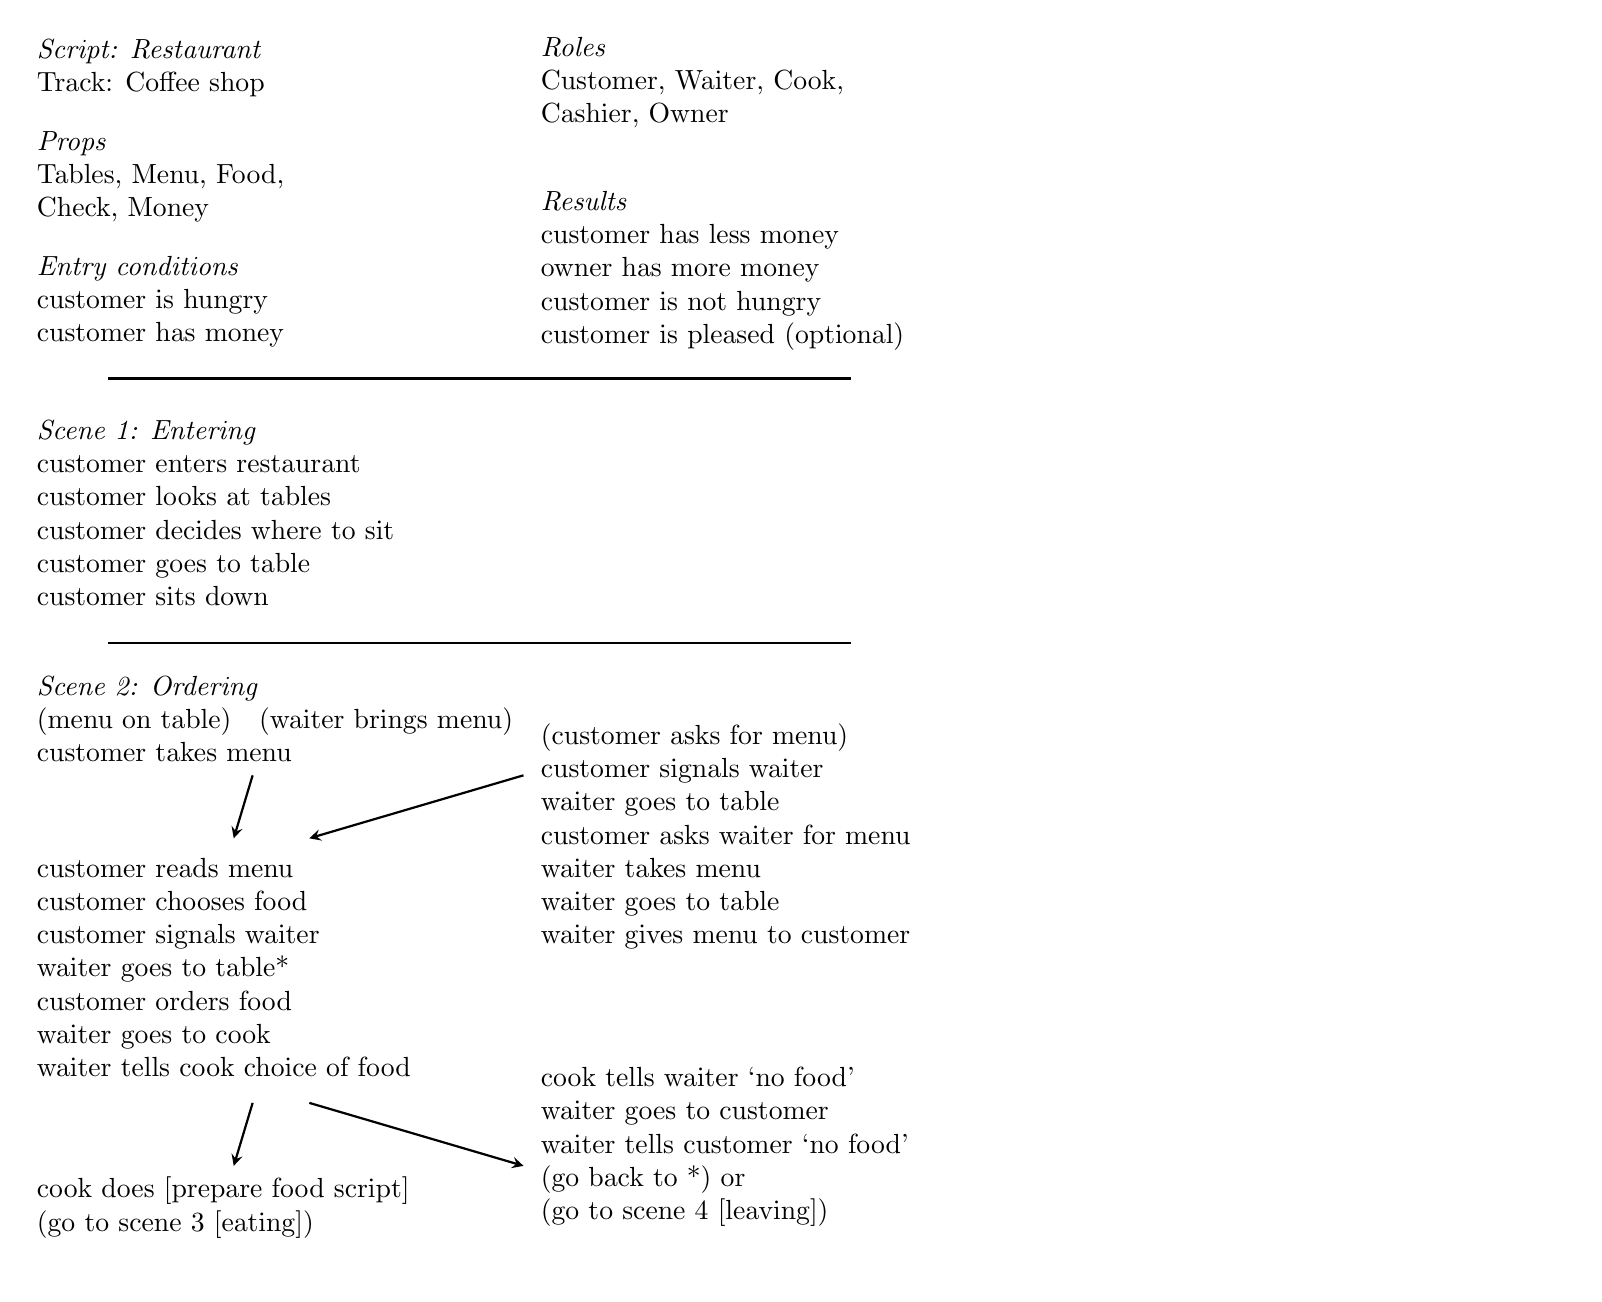
\begin{tikzpicture}[scale=.8]

\node (header) at (0,7.7) {
\begin{minipage}{13cm}
\textit{Script: Restaurant}\\
Track: Coffee shop\\
\end{minipage}
};

\node (props) at (0,6.2) {
\begin{minipage}{13cm}
\textit{Props}\\
Tables, Menu, Food, \\
Check, Money
\end{minipage}
};

\node (roles) at (8,7.7) {
\begin{minipage}{13cm}
\textit{Roles}\\
Customer, Waiter, Cook, \\
Cashier, Owner
\end{minipage}
};

\node (conditions) at (0,4) {
\begin{minipage}{13cm}
\textit{Entry conditions}\\
customer is hungry\\
customer has money\\
\end{minipage}
};

\node (results) at (8,4.5) {
\begin{minipage}{13cm}
\textit{Results}\\
customer has less money\\
owner has more money\\
customer is not hungry\\
customer is pleased (optional)\\
\end{minipage}
};

\node (entering) at (0,0.6) {
\begin{minipage}{13cm}
\textit{Scene 1: Entering}\\
customer enters restaurant\\
customer looks at tables\\
customer decides where to sit\\
customer goes to table\\
customer sits down\\
\end{minipage}
};

\node (ordering1) at (0,-2.4) {
\begin{minipage}{13cm}
\textit{Scene 2: Ordering}\\
(menu on table)~~~(waiter brings menu)\\
customer takes menu
\end{minipage}
};

\node (ordering2) at (8,-4.49) {
\begin{minipage}{13cm}
(customer asks for menu)\\
customer signals waiter\\
waiter goes to table\\
customer asks waiter for menu\\
waiter takes menu\\
waiter goes to table\\
waiter gives menu to customer\\
\end{minipage}
};

\node (ordering3) at (0,-6.5) {
\begin{minipage}{13cm}
~~\\
customer reads menu\\
customer chooses food\\
customer signals waiter\\
waiter goes to table*\\
customer orders food\\
waiter goes to cook\\
waiter tells cook choice of food  \\
\end{minipage}
};

\node (ordering4) at (8,-9.2) {
\begin{minipage}{13cm}
cook tells waiter `no food'\\
waiter goes to customer\\
waiter tells customer `no food'\\
(go back to *) or\\
(go to scene 4 [leaving])
\end{minipage}
};

\node (ordering5) at (0,-10.37) {
\begin{minipage}{13cm}
cook does [prepare food script]\\
(go to scene 3 [eating])\\
\end{minipage}
};

\draw[thick] (-7,3) -- (4.8,3);
\draw[thick] (-7,-1.2) -- (4.8,-1.2);
\draw[thick, -stealth] (-4.7,-3.3) -- (-5,-4.3);
\draw[thick, -stealth] (-.4,-3.3) -- (-3.8,-4.3);
\draw[thick, -stealth] (-4.7,-8.5) -- (-5,-9.5);
\draw[thick, -stealth] (-3.8,-8.5) -- (-0.4,-9.5);

\end{tikzpicture}
\caption{Extract of the restaurant script based on \citet[43]{schank.abelson1977}. For expository purposes, I replaced the CDT representations by natural language counterparts and simplified Scene 2.\label{fig:restaurant-script-schank.abelson}}
\end{figure}

First, each script\is{Script knowledge} has a \textit{header} (``Restaurant''), a set of \textit{roles} identifying the participants involved in the script\is{Script knowledge}, and a set of \textit{props}, i.e. objects that typically appear in that script\is{Script knowledge}. A script\is{Script knowledge} can have several \textit{tracks}, for instance, \citet[40--41]{schank.abelson1977} distinguish a ``fancy restaurant track'' and a ``fast-food track'' in order to account for differing sets of props, roles, events, and ordering thereof depending on the type of restaurant. Scripts\is{Script knowledge} are activated by their necessary \textit{entry conditions} and lead to a set of \textit{results}, some of which might be optional. If the entry conditions are not satisfied, e.g. when a customer who is not hungry or who has no money goes to the restaurant, the events will not follow their stereotypical time-course, so that applying the script\is{Script knowledge} will not yield a benefit in comprehension. The results follow from the application of a script\is{Script knowledge} or a particular version thereof.

\citet{schank.abelson1977} assume that script\is{Script knowledge} events are hierarchically grouped into \textit{scenes}. For instance, they divide the restaurant script\is{Script knowledge} into entering, ordering, eating and exiting scenes.%
%
\footnote{There is some experimental evidence that scripts\is{Script knowledge} are indeed represented as hierarchical structures in memory. For instance, \citet{bower.etal1979} report a segmentation task on script\is{Script knowledge} data suggesting that subjects agree to a large extent on the placement of boundaries between script\is{Script knowledge} events. They argue that this indicates a natural segmentation of scripts\is{Script knowledge} into scenes. \citet{abbott.etal1985} present a memory recall task that evidences a distinction in asymmetric priming between script\is{Script knowledge} events and scene headers: While the former facilitate the recall of the latter, this does not hold vice versa. More recently, a similar structure has been assumed by \citet{cooper.shallice2000} in order to model errors in script\is{Script knowledge}-based behavior, but see \citet{botvinick.plaut2004} for a non-hierarchical account. As all of my materials involve a sequence of three consecutive script\is{Script knowledge} events on the same granularity level, both flat and hierarchical script\is{Script knowledge} models predict that the next event will be activated. I hence remain agnostic with respect to the precise representation of script knowledge\is{Script knowledge} in memory.}\afterfn%
%
Each scene in turn comprises a set of (partially) ordered events. Although many events in the restaurant follow each other obligatorily, the ordering of events within a scene is neither complete, nor is the path to be followed through each scene fully linear. The \textit{entering} scene is described as fully linear, but the \textit{ordering} scene can develop in different ways depending on whether the menu is on the table when the customers sit down. If the waiter does not bring food to the customer, it is either possible to return to the food choice event or to skip the \textit{eating} scene and proceed with \textit{leaving}. I address this partially nonlinear ordering of events by estimating their likelihood in the context of the previous one(s) from a script\is{Script knowledge} corpus\is{Corpus}.

\subsubsection{Scripts as primes for upcoming material}
This brief sketch of \citepos{schank.abelson1977} view on scripts\is{Script knowledge} suggests that scripts\is{Script knowledge} are a promising approximation to extralinguistic context\is{Context, extralinguistic}. Since scripts\is{Script knowledge} about everyday events are shared by a wide part of the population, and their representation is relatively homogeneous between individuals \citep{bower.etal1979}, it is reasonable to assume that a script\is{Script knowledge} evokes similar predictions within at least most of the participants in an experiment. \is{Event chain|(}As I discuss in greater detail in the next section, the basic idea underlying my experiments is to manipulate the likelihood of a target event with a script\is{Script knowledge}-based context story. \Next exemplifies the structure of a sample item used in experiment \ref{exp:scripts-rating} for the pasta cooking script\is{Script knowledge}. The context story consists of a  sentence referring to the script\is{Script knowledge} title \Next[a] and a sequence of the three immediately preceding events \Next[b--d].%
%
\footnote{For details on how this structure is generated and why other potential script\is{Script knowledge} events such as \textit{grab a large pot} or \textit{open the pasta package} are not included, see Section \ref{sec:infotheory-scr-corpus-preprocessing}.}\afterfn% 
%
\is{Event chain|)}Given this context story, I expect script\is{Script knowledge} events \Next[e] that are likely in that context to be more predictable than non-script events \Next[f]. This setting allows for the investigation of the hypothesis that utterances referring to predictable events are more likely to be reduced.

\ex.  \label{ex:scripts-item-abstract}
\a. cook pasta \hfill Script title
    \b. put pot with water on stove \hfill Context event 1
    \c. turn stove on\hfill Context event 2
    \d. water boils\hfill Context event 3
    \e. pour pasta into pot\hfill Target event
    \f. set table \hfill Non-script event

Based on \citepos{schank.abelson1977} theory, it seems natural to assume that \Last[e] is predictable in  the context of \Last[a--d], however, it needs to be empirically shown that this is indeed the case. Fortunately, a large bulk of experimental studies indicates that text comprehension involves the generation of predictive inferences about upcoming material \citep[see e.g.][]{bower.etal1979, mckoon.ratcliff1986, vandenbroek1994, vandermeer.etal2002, nuthmann.vandermeer2005,camblin.etal2007, otten.vanberkum2007, hare.etal2009, bicknell.etal2010, matsuki.etal2011,metusalem.etal2012, delogu.etal2018}. For instance, \citet{bower.etal1979} find that sentences referring to script\is{Script knowledge} events are read faster when they follow the immediately preceding event in the script\is{Script knowledge}, as compared to contexts where one or two events in between them are omitted. This suggests that subjects generate expectations that constrain processing\is{Processing effort} as they read script\is{Script knowledge}-based stories. More recently, \citet{vandermeer.etal2002} show that the priming effect of script knowledge\is{Script knowledge} is stronger for upcoming events. Taken together, previous research on script knowledge\is{Script knowledge} predicts that the context story in \Last[a--d] will indeed prime the target event in \Last[e] as compared to the unrelated \Last[f].\is{Script knowledge|)} In what follows, I explain how the likelihood of an event in context was calculated based on the DeScript corpus\is{Corpus} of script knowledge\is{Script knowledge}.

\subsection{Estimating event surprisal from script corpora}
\label{sec:infotheory-script-event-chains}

\subsubsection{Scripts as probabilistic event chains}
\is{Event chain|(}The script\is{Script knowledge} representations underlying the materials for experiments \ref{exp:scripts-rating} and \ref{exp:scripts-production} model scripts\is{Script knowledge} as probabilistic networks rather than as linear event sequences, as most of the previous work on scripts\is{Script knowledge} did. In such a network, each event is assigned a state $e_i$ which has a transition probability to another state $e_j$. The transition probability $p(e_j\mathbin{|}e_i)$ indicates the likelihood of $e_j$ to follow $e_i$ and can be estimated for each pair of states $\langle e_i,e_j\rangle$ {}in the total set of states that is determined by the script\is{Script knowledge}. The transition probabilities can range from 0, i.e. $e_j$ never follows $e_i$, to 1 in case $e_j$ always follows $e_i$. Figure \ref{fig:script-abstract} shows a part the abstract representation of the pasta scenario. Based on the transition probabilities it is possible to extract a linear sequence of the most likely events to follow each other even though the underlying structure itself is nonlinear. For instance, the four events marked in grey in Figure \ref{fig:script-abstract} were used to build the item for the pasta scenario given in \ref{ex:scripts-item-abstract}.\is{Event chain|)}

\begin{figure}[t]
  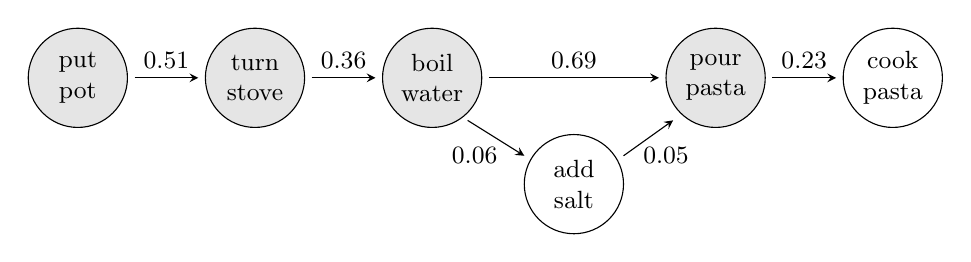
\begin{tikzpicture}[scale=.9]
{\small
\fill [black!10!] (0,0) circle [radius=.7];
\fill [black!10!] (2.5,0) circle [radius=.7];
\fill [black!10!] (5,0) circle [radius=.7];
\fill [black!10!] (9,0) circle [radius=.7];
\fill [white] (7,-1.5) circle [radius=.7];
\fill [white] (11.5,0) circle [radius=.7];

\draw [black] (0,0) circle [radius=.7] node[align=center]{put\\pot};
\draw [black] (2.5,0) circle [radius=.7] node[align=center]{turn\\stove};
\draw [black] (5,0) circle [radius=.7] node[align=center]{boil\\water};
\draw [black] (9,0) circle [radius=.7] node[align=center]{pour\\pasta};
\draw [black] (7,-1.5) circle [radius=.7] node[align=center]{add\\salt};
\draw [black] (11.5,0) circle [radius=.7] node[align=center]{cook\\pasta};

\draw [-stealth] (.8,0) -- (1.7,0) node [midway, above] {0.51};
\draw [-stealth] (3.3,0) -- (4.2,0) node [midway, above] {0.36};
\draw [-stealth] (5.8,0) -- (8.2,0) node [midway, above] {0.69};
\draw [-stealth] (9.8,0) -- (10.7,0) node [midway, above] {0.23};
\draw [-stealth] (5.5,-0.6) -- (6.3,-1.1) node at (5.6,-1.1){0.06};
\draw [-stealth] (7.7,-1.1) -- (8.4,-0.6) node at (8.3,-1.1){0.05};

}
\end{tikzpicture}
 \caption{Sample event chain with transition probabilities between events estimated from the preprocessed DeScript data. The four events marked in grey were used in the item for the pasta scenario in experiment \ref{exp:scripts-rating}.\label{fig:script-abstract}}
\end{figure}

The usage of probabilistic structures has conceptual and methodological advantages over hand-crafted script\is{Script knowledge} structures like the restaurant script\is{Script knowledge} sketched in Figure \ref{fig:restaurant-script-schank.abelson} above. First, probabilistic structures might be more empirically appropriate descriptions of  differing representations of the same script\is{Script knowledge} within the population. Intuitions of an individual researcher might deviate from the overall most likely time-course of events, and averaging over data from about 100 contributors to the corpus\is{Corpus} data for each script\is{Script knowledge} is a better approximation to the general expectations about a script\is{Script knowledge}. Second, probabilistic event chain\is{Event chain}s model the uncertainty about upcoming events in the script\is{Script knowledge}. Even in the detailed sketch of the restaurant script\is{Script knowledge} by \citet{schank.abelson1977} there is no fully linear order but several branchings, for instance the waiter might serve the customer the intended dish or not. Speakers might have probabilistic expectations about which of these continuations is more likely, and these expectations must be quantified when it comes to estimating the likelihood of upcoming events. This uncertainty is a property of scripts\is{Script knowledge} even if a single speaker has a fully deterministic view on it. For instance, a person who always prepares scrambled eggs in the same way has knowledge about how others do it. If scripts\is{Script knowledge} are used in the comprehension of new stories, it seems reasonable to rely not only on individual preferences: A hearer will expect with a certain probability that bacon, vegetables or spices are added. 
Finally, transition probabilities between events can be estimated from script\is{Script knowledge} corpora\is{Corpus}. In contrast, if the ordering between two events is reverted only once in the corpus\is{Corpus}, a linear order cannot be established. Taken together, all of these issues favor the resort to probabilistic representations of scripts\is{Script knowledge} that I use in my studies. In the remainder of Section \ref{sec:infotheory-scripts}, I describe the procedure that I used to extract context stories like that given above from the DeScript corpus\is{Corpus} of script knowledge\is{Script knowledge} \citep{wanzare.etal2016}.

\subsubsection{Selection of scripts from the DeScript corpus}
The experiments presented in this chapter are based on data extracted from the DeScript corpus\is{Corpus} \citep{wanzare.etal2016}. DeScript has been crowdsourced on Amazon Mechanical Turk and comprises about 100 event-sequence descriptions (ESD\is{Event sequence description}s) by native speakers of English\il{English} for each of 40 scripts\is{Script knowledge}. The corpus\is{Corpus} is freely available in XML format and is partially annotated for coreferences between script\is{Script knowledge} events. The scripts\is{Script knowledge} contained in the corpus\is{Corpus} differ both in their internal complexity (e.g. \textit{washing dishes} and \textit{going to a funeral}), that is, variation between (the number of) events and their order as well as with respect to the number of participants involved. 

The corpus also contains both what \citet{schank.abelson1977} termed situational and instrumental scripts\is{Script knowledge}, between which \citet{schank.abelson1977} assume a categorical distinction. Instrumental scripts\is{Script knowledge} ``usually'' have only one participant \citep[65]{schank.abelson1977}, and the order of events in the script\is{Script knowledge} is more fixed than in situational ones. As examples of instrumental scripts\is{Script knowledge}, they list scripts\is{Script knowledge} like \textit{lighting a cigarette}, \textit{starting a car} or \textit{frying an egg}. According to \citet[66]{schank.abelson1977}, a consequence of this (apparently gradual) structural difference is that instrumental scripts\is{Script knowledge} do not make use of ``powerful predictive mechanisms'' and that their details are forgotten faster than those of situational scripts\is{Script knowledge} as the story unfolds. As \citet[66]{schank.abelson1977} put it, ``[w]e simply don't expect that `I fried an egg' is the beginning of a story about an interesting thing that happened in the process of egg frying.'' If the predictive potential of both script\is{Script knowledge} types differed, this could potentially affect the outcome of the experiments. 

Since my experiments investigate encoding preferences for utterances, it was necessary that (at least) two characters participate in the script\is{Script knowledge}. This was not the case for the instrumental scripts\is{Script knowledge} in DeScript, leaving at most 17 scripts\is{Script knowledge} that involved a second participant. 
In order to test six trials per condition in experiment \ref{exp:scripts-rating} in a 2$\times$2 design, I required 24 scripts\is{Script knowledge} that involved at least two participants. Therefore, I adapted some of the scripts\is{Script knowledge} that originally did not contain a second participant, but for which it is reasonable to assume that the script\is{Script knowledge} would not be significantly changed by the introduction of such an additional character. For instance, in the pasta cooking scenario, it is very plausible that a couple, roommates or friends prepare a meal together and talk in the meantime. Consequently, I chose 24 scenarios from DeScript that best met this requirement.


Therefore, I included a binary control predictor \textsc{ScriptType} in the statistical analysis of experiment \ref{exp:scripts-rating} that (i) shows whether one of these script\is{Script knowledge} types is more predictive than the other one, and that (ii) if so, allows me to factor out this effect. Anticipating the results, there is no significant difference between script\is{Script knowledge} types with respect to their predictive potential.

\subsubsection{Estimating event probabilities}
\label{sec:infotheory-scr-corpus-preprocessing}
\is{Event chain|(}Estimating the likelihood of an event in context of the preceding one(s) requires transforming the representations provided by the contributors\is{Event sequence description} to the corpus\is{Corpus} into event chains\is{Event chain}. After that, the likelihood of an event can be estimated with \textit{n}-gram language models\is{N-gram language model}. Since in this case the primitive expressions are event labels instead of natural language words, I refer to his procedure as \textit{event sequence\is{Event chain} modeling}, even though it is technically identical to the modeling of natural language data. Event sequence modeling requires that each event in the relevant corpus\is{Corpus} data is assigned a unique label that distinguishes it from other events. In what follows I describe how I preprocessed the DeScript data for the selected 24 scenarios in order to construct materials for experiments \ref{exp:scripts-rating} and \ref{exp:scripts-production}.

Following \citet{manshadi.etal2008}, event labels consisted of the main verb of each event description and the post-verbal noun, which is its direct object in case of transitives.%
%
\footnote{More sophisticated methods for representing script\is{Script knowledge} events can take into account the semantic role of a character with respect to the verb \citep{chambers.jurafsky2008}, use skip-grams\is{Skip-gram language model} \citep{jans.etal2012} or include multiple arguments for each verb \citep{chambers.jurafsky2009, pichotta.mooney2014}. These approaches outperform simpler approaches in evaluation tasks in computational linguistics, but for my purpose of assigning each event a distinctive label taking the verb and post-verbal noun as event representation was sufficiently accurate.}\afterfn%
%
The corpus\is{Corpus} data were therefore preprocessed in order to obtain event representations like \Next, based on which event probabilities\is{Event chain} were estimated. Note that for the purpose of event sequence\is{Event chain} modeling, it does not matter whether e.g. \texttt{turn stove} is the most accurate description of the event of turning the stove on:  As long as the same label is assigned to all instances of the corresponding event and to no instance of any different event, the model will correctly determine the likelihood of the corresponding event. 

\ex. \texttt{put pot}~~~\texttt{turn stove}~~~\texttt{boil water}~~~\texttt{pour pasta}  

The event descriptions in DeScript are diverse in various respects. First, script knowledge\is{Script knowledge} differs between individuals, who might perform the same script\is{Script knowledge}, e.g. cooking pasta or scrambled eggs, in a different fashion. Second, descriptions that do not differ in the nature and time-course of events sometimes do so in precision and granularity. Some subjects mention that they turn on the stove or take the pan out of the cupboard, while others begin the ESD\is{Event sequence description} with breaking up the eggs into the pan. Sometimes these omissions concern events that are necessary conditions for the following events: Even if picking a pan is not mentioned, this must have happened at the point where the eggs are broken inside it. Finally, descriptions of the same event differ with respect to the lexical items chosen, pronominalizations and ellipses, as the examples from DeScript in \Next show.

\ex.    \label{ex:scripts-synonym}
\a. Pour eggs into the pan
\b. Put contents of bowl in pan
      \c. Pour them into a pan
      \d. Pour in pan

To some extent, this diversity is a property inherent to script knowledge\is{Script knowledge}, specifically with respect to different stereotypical orders of events between speakers. Since my UID\is{Uniform Information Density} account of fragment usage implies that speakers engage in audience design\is{Audience design}, whenever this adaption concerns script knowledge\is{Script knowledge}, the speaker must adapt her utterance to the (inferred) script knowledge\is{Script knowledge} of the hearer rather than to her own. Consequently, she must infer which expectations about the script\is{Script knowledge} the hearer has. Under the assumption that the sample of script\is{Script knowledge} representations for a given scenario in DeScript comes close to being representative for an average hearer, differences between the probability of events in the DeScript data will reflect relevant differences in likelihood of events given a generic hearer. Therefore, modeling the likelihood and ordering of events reflects psychologically relevant aspects of script knowledge\is{Script knowledge}. The opposite arguably holds for differences in lexical choice or syntactic constructions when describing the individual events. All of the descriptions in \Last refer to the same event of pouring the eggs into the pan, consequently they should be treated as the same event in event sequence\is{Event chain} modeling. This requires a notable amount of preprocessing, that I describe in greater detail below. Differences in granularity are probably a case somewhere between actual diversity between script\is{Script knowledge} representations, which needs to be reflected in the event chains\is{Event chain} and linguistic variance in the corpus\is{Corpus}-based descriptions. On the one hand, it could be argued that in a sequence like \Next a stove and a pan are necessarily involved, and that the pan must have been put on the stove and heated in order to cook the eggs. On the other hand, I use the event chain\is{Event chain}s as an approximation to the likelihood of events being referred to by an utterance, and events that are considered irrelevant enough to be omitted in an ESD\is{Event sequence description} might not be likely enough to be talked about. Therefore, I did not assimilate the ESD\is{Event sequence description}s with respect to granularity. Furthermore, doing so would involve a high degree of arbitrariness when it comes to deciding whether an event is necessary in the time-course of the script\is{Script knowledge} or not. 

\ex. \a. Break two eggs in a bowl
\b. Get a whisk
\c. Whisk eggs together till they are light and fluffy
\d. Add a bit of milk
\e. Start cooking eggs

\begin{figure}[t]
 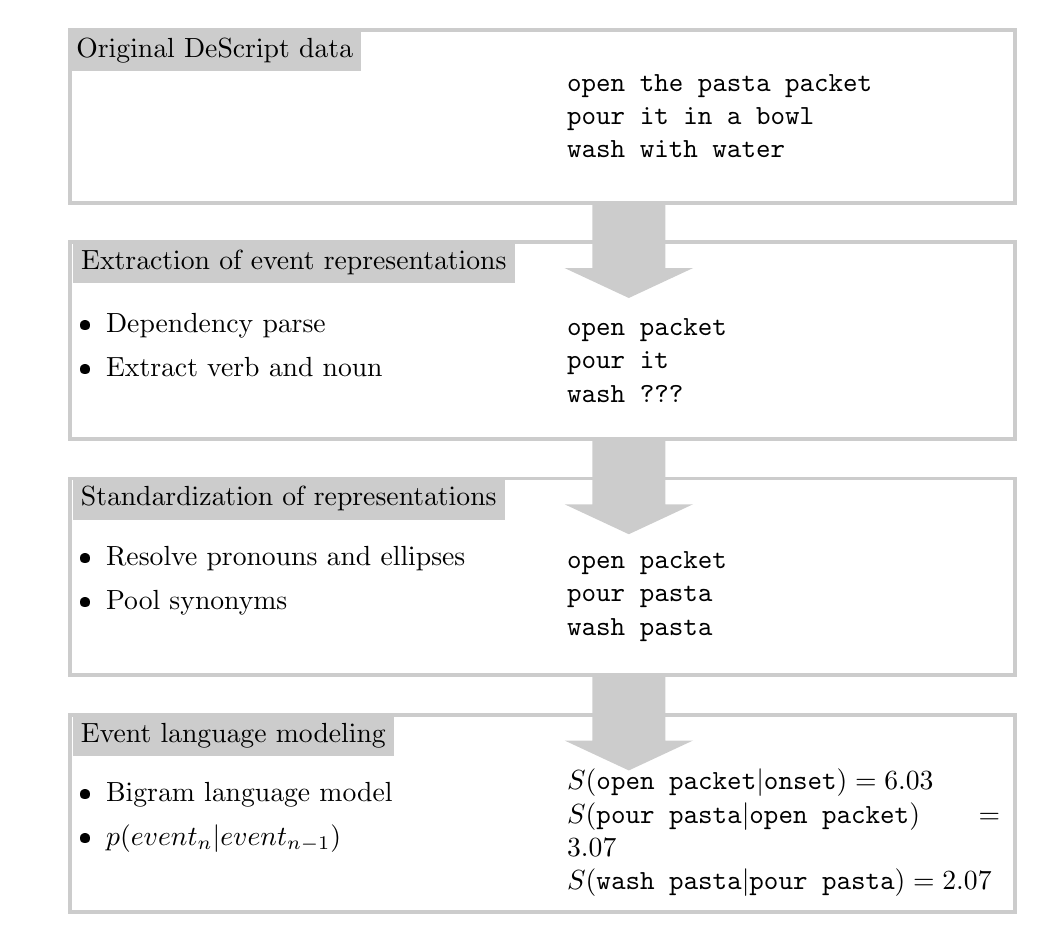
\begin{tikzpicture}[scale=1]

 \draw [draw = black!20!, line width = .5mm] (0,-.3) rectangle (12,-2.5);
\node (t) at (1.84,-.56) [fill = black!20!, inner sep = 3pt] {Original DeScript data};
\node (mp) at (5.7,-1.4){
\begin{minipage}{6cm}
~~
\end{minipage}
\begin{minipage}{.5cm}
 ~~
\end{minipage}
\begin{minipage}{5.5cm}
\texttt{open the pasta packet}\\
\texttt{pour it in a bowl}\\
\texttt{wash with water}
\end{minipage}

};

\draw [draw = black!20!, line width = .5mm] (0,-3) rectangle (12,-5.5);
\node (t) at (2.846,-3.26) [fill = black!20!, inner sep = 3pt] {Extraction of event representations};
\node (mp) at (5.7,-4.5){
\begin{minipage}{6cm}
\vspace{-.4cm}
\begin{itemize} \itemsep0em
  \item Dependency parse
 \item Extract verb and noun
\end{itemize}
\end{minipage}
\begin{minipage}{.5cm}
 ~~
\end{minipage}
\begin{minipage}{5.5cm}
\texttt{open packet}\\
\texttt{pour it}\\
\texttt{wash ???}
\end{minipage}

};

\draw [draw = black!20!, line width = .5mm] (0,-6) rectangle (12,-8.5);
\node (t) at (2.781,-6.26) [fill = black!20!, inner sep = 3pt] {Standardization of representations};
\node (mp) at (5.7,-7.5){
\begin{minipage}{6cm}
\vspace{-.4cm}
 \begin{itemize} \itemsep0em
  \item Resolve pronouns and ellipses
 \item Pool synonyms
\end{itemize}
\end{minipage}
\begin{minipage}{.5cm}
 ~~
\end{minipage}
\begin{minipage}{5.5cm}
\texttt{open packet}\\
\texttt{pour pasta}\\
\texttt{wash pasta}
\end{minipage}

};

\draw [draw = black!20!, line width = .5mm] (0,-9) rectangle (12,-11.5);
\node (t) at (2.078,-9.26) [fill = black!20!, inner sep = 3pt] {Event language modeling};
\node (mp) at (5.7,-10.5){
\begin{minipage}{6cm}
\vspace{-.4cm}
 \begin{itemize} \itemsep0em
  \item Bigram language model
  \item $p(event_n|event_{n-1})$
\end{itemize}
\end{minipage}
\begin{minipage}{.5cm}
 ~~
\end{minipage}
\begin{minipage}{5.5cm}
$S(\texttt{open packet}|\texttt{onset}) = 6.03$\\
$S(\texttt{pour pasta}|\texttt{open packet}) = 3.07$\\
$S(\texttt{wash pasta}|\texttt{pour pasta}) = 2.07$
\end{minipage}

};

\node at (7.1,-3)[single arrow, single arrow head extend=10pt, single arrow tip angle=130, shape border rotate=270,inner sep=8pt, fill=black!20!, minimum height=1.2cm]{~~~~};
\node at (7.1,-6)[single arrow, single arrow head extend=10pt, single arrow tip angle=130, shape border rotate=270,inner sep=8pt, fill=black!20!, minimum height=1.2cm]{~~~~};
\node at (7.1,-9)[single arrow, single arrow head extend=10pt, single arrow tip angle=130, shape border rotate=270,inner sep=8pt, fill=black!20!, minimum height=1.2cm]{~~~~};

\end{tikzpicture}
\caption{Overview of the preprocessing procedure for a sample sequence of events from DeScript.\label{fig:scripts-preprocessing}}
\end{figure}
%
The lexical and syntactic variation within the event descriptions in DeScript requires the assimilation of these descriptions, so that a single label is assigned to each event. For this purpose, the corpus\is{Corpus} data were pre-processed using a semi-automatic approach that is summarized in Figure \ref{fig:scripts-preprocessing} and described in what follows. After preprocessing, each instance of each event is assigned a unique label, so that event sequence\is{Event chain} models can be used to estimate its probability to occur in context. The labels for events were generated by first extracting the main verb and its complement noun from the event descriptions in DeScript. For this purpose, the raw DeScript data were Part of Speech-tagged with the Stanford parser \citep{klein.manning2003} for English\il{English} contained in the Python Natural Language Toolkit (NLTK) \citep{loper.bird2002}. The data were then dependency-parsed using the Stanford dependency parser contained in the NLTK. The parser was often misguided by the high ratio of elliptical event descriptions, subject omission\is{Subject drop}s and verb-first imperatives that are infrequent in the written corpora\is{Corpus} on which it was trained. In such situations, it interprets e.g. initial verbs as nouns, specifically when there are homonymous with nouns like \textit{set} and then assigns wrong POS tags to following words. This was addressed by using a language model file trained by Micaela Regneri and Ines Rehbein on a modified set of training corpora\is{Corpus} from which some of the sentence-initial noun phrases\is{Noun phrase} had been removed.%
%
\footnote{See \citet[49--50]{regneri2013} for details. I thank Simon Ostermann for suggesting this approach and sharing the model file trained on the modified corpora\is{Corpus}.}\afterfn%
%
This method allows the parser to analyze English\il{English} SVO structures with missing subjects as such instead of analyzing initial verbs as nouns and results in a higher accuracy of the parser. After parsing, the main verb and its direct object were extracted using Python scripts. In case there was no direct object, a placeholder was inserted and reviewed manually.%
% 
\footnote{I thank Lisa Schäfer for her suggestions and ideas that significantly influenced the methods described in this section.}\afterfn%
%
The resulting \texttt{verb noun} event representations for each scenario were further manually preprocessed in order to pool synonym words and syntactically differing descriptions of the same event. The rationale for this procedure was that (i) each script\is{Script knowledge} should involve a set of mutually exclusive participants (both animate and inanimate, i.e. roles and props in the terminology in \citet{schank.abelson1977}), that there should be a unique label for each participant, and that (ii) the same held for events, so there should be a unique label for each event within the script\is{Script knowledge}.%
%
\footnote{This idea of preprocessing elicited script\is{Script knowledge} data is not fully new. \citet{bower.etal1979} started their series of experiments on script knowledge\is{Script knowledge} by collecting natural data on knowledge about five scripts\is{Script knowledge}. Subjects provided list descriptions of the events involved in the stereotypical time-course of each script\is{Script knowledge}, thus yielding data relatively similar to current script\is{Script knowledge} corpora\is{Corpus}. The data provided for each script\is{Script knowledge} (there were between 24 and 37 subjects and consequently descriptions per script\is{Script knowledge}) were preprocessed by unifying ``paraphrases and synonyms'' \citep[181]{bower.etal1979} and then used to build ordered event lists comprising events mentioned by more than 25\% of the respective subjects. Except for the smaller number of scripts\is{Script knowledge} and participants per script\is{Script knowledge}, this procedure anticipates the collection of script knowledge\is{Script knowledge} in more recent corpora\is{Corpus} of script knowledge\is{Script knowledge} (see Section \ref{sec:infotheory-script-event-chains}) and the preprocessing approach that I apply to such data.%
\label{fn:bower-etal-ex1}}\afterfn%
%
The first requirement ensures that synonyms, such as \textit{pan} and \textit{skillet}, were pooled to a single lemma, whereas the second one requires the same label to be assigned to different descriptions of the same action, like those given in \ref{ex:scripts-synonym}. This is crucial for interpreting the event sequence\is{Event chain} models calculated on these representations, because otherwise the probability mass of e.g. the event referring to pouring the eggs into the pan would be split among the events \texttt{pour egg}, \texttt{put content} and \texttt{pour in}. In order to obtain unique labels for each event, it was also necessary to resolve ellipses and the reference of pronouns. Finally, the data for each scenario were screened using an \texttt{R} script in order to ensure the uniqueness of each participant, each action, and consequently each event within the script\is{Script knowledge}.

After preprocessing, the likelihood of each event was estimated with bigram\is{Bigram language model} event sequence\is{Event chain} models with Good-Turing discounting using the SRILM toolkit \citep{stolcke2002}. In contrast to the language modeling approaches discussed so far, the primitives are not words, but events, and the models return the probability of an event given the previous one (or the script\is{Script knowledge} onset) based on representations like \Last. The usage of higher order \textit{n}-grams\is{N-gram language model} would not have been reasonable given the relatively small amount of data of about 100 ESDs per scenario. Even after preprocessing, relatively homogeneous scenarios such as \textit{train ride} had a vocabulary size (the number of different primitive events) of 121, more diverse scenarios, such as e.g. \textit{making scrambled eggs} even had a unigram\is{Unigram language model} vocabulary size of 192. As there is often more than one possible successor for each event, this yields a vocabulary of 351 bigram\is{Bigram language model}s for the train and of 672 bigram\is{Bigram language model}s for the eggs scenario.\is{Event chain|)}

Preprocessing the DeScript data for 24 scripts\is{Script knowledge} using automatized and manual procedures yielded a high-quality data set that I used to estimate the likelihood of script\is{Script knowledge}-based events. The method described in this section ensures that the probability mass of an event is not split among alternative lexicalizations, and that speakers' script knowledge\is{Script knowledge} is a probabilistic estimate of how people represent a particular script\is{Script knowledge}, including differences in the events involved, their ordering and granularity. I used these probabilistic representations of script knowledge\is{Script knowledge} to construct the materials for experiments \ref{exp:scripts-rating-case}, \ref{exp:scripts-rating} and \ref{exp:scripts-production}.

\refstepcounter{expcounter}\label{exp:scripts-rating}
\section{Experiment \ref{exp:scripts-rating}: Script knowledge, rating}  \label{sec:scripts-rating}

\subsection{Background}
Experiment \ref{exp:scripts-rating} tests the densification prediction in clause \ref{ex:uid-pred-density} that fragments are more strongly preferred in predictive contexts, which according to UID\is{Uniform Information Density}, results from the tendency to omit predictable words in order to avoid troughs in the ID profile. Empirical evidence for this prediction will also show that the script\is{Script knowledge}-based predictability manipulation works at all. This is a requirement for using the same stimuli in the production task\is{Production task} in experiment \ref{exp:scripts-production} that investigates the predictions of UID\is{Uniform Information Density} on omissions on the more fine-grained word level.

\subsection{Materials}\label{sec:scripts-rating-materials}

Experiment \ref{exp:scripts-rating} compares the acceptability\is{Acceptability rating task} of predictable and unpredictable DP\is{Determiner phrase} fragments \Next[a,b] to that of corresponding full sentences \Next[c,d] in  2$\times$2 design (\textsc{Pre\-dictability} $\times$ \textsc{Sententiality}) in a rating study\is{Acceptability rating task}.%
%
\footnote{The experiment was conducted in German, but I provide an English translation of the context story here for convenience.}\afterfn%
%

\ex. Annika and Jenny want to cook pasta. Annika put a pot with water on the stove. Then she turned the stove on. After a few minutes, the water started to boil. Now Annika says to Jenny: \label{ex:scripts-rating-item}
     \ag.  Die Nudeln, bitte.\\
	  the pasta please\\
	  \trans{The pasta, please.} \exsourceraised{Predictable}
     \bg. Den Küchentisch, bitte.\\
	  the.\textsc{acc} kitchen.table please\\
	  \trans{The kitchen table, please.} \exsourceraised{Unpredictable}
     \cg. Schütte die Nudeln ins Wasser, bitte.\\
	  pour the pasta in.the water please\\
	  \trans{Pour the pasta into the water, please.}\exsourceraised{Predictable}
     \dg. Deck schon mal den Küchentisch, bitte.\\
	  set already \textsc{prt} the.\textsc{acc} kitchen.table please\\
	  \trans{Set the kitchen table, please.}\exsourceraised{Unpredictable}

The script\is{Script knowledge}-based context story is identical for all conditions. The target utterance in the predictable conditions always refers to the most likely event in the context of the story (\texttt{pour pasta} in the example). In the unpredictable conditions, it refers to an event that did not appear in the script\is{Script knowledge} data at all, or that has a probability of 0 in this context, but that is intuitively not implausible to be talked about in the situation described by the context story. The idea that underlies this approach is that probable events are more likely to be referred to with an utterance than unpredictable ones.\largerpage%
%
\footnote{Using the probability of an event as a proxy for that of an utterance is a simplification, and \textit{very} likely events might actually \textit{not} be talked about because they are so obvious. However, experiment \ref{exp:scripts-production} confirms that predictable events are more likely to be talked about.}\footnote{In order to rule out the possibility that differences between the \textsc{Predictability} conditions concern other factors than predictability, it would have been desirable to test the \textit{same} utterance in a predictive and an unpredictive context. However, due to the usage of script\is{Script knowledge} corpus\is{Corpus} data, the only possible method was to construct one story per item and to vary the utterance between \textsc{Predictability} conditions. If new (unpredictable) contexts were constructed from scratch, it would have been impossible to estimate the likelihood of the target utterance in the same way as for the corpus\is{Corpus}-based stories. Therefore, I used one context story by item and varied the target utterance between \textsc{Predictability} conditions. Potential differences between both utterances are furthermore accounted for by by-item random slopes for \textsc{Predictability} in the statistical analysis.}\afterfn%
%
Each context story consists of four sentences, the first of which introduced to the script\is{Script knowledge} and mentioned its title, e.g. \textit{cook pasta}.%
% 
\footnote{\citet{schank.abelson1977} argue that scripts\is{Script knowledge} are only accessed for text comprehension after their \textit{activation} and \textit{instantiation}. They assume that it were implausible that possibly hundred of scripts\is{Script knowledge} are always active at the same time, but that scripts\is{Script knowledge} are only activated when their \textit{header} is encountered. In the sample item, the header is \textit{cook pasta} in the first sentence of the context story. According to \citet[47--48]{schank.abelson1977}, instantiation consists in copying the complete script\is{Script knowledge} to working memory, so that its components can be accessed during the comprehension of linguistic input. In the theory, instantiation occurs when a subsequent sentence fits the structure of an activated script\is{Script knowledge}, i.e. the hearer encounters a script\is{Script knowledge} event. Even though this distinction is controversial \citep[see e.g.][]{rabs.etal2017}, in the experimental stimuli each script\is{Script knowledge} should be active and instantiated after processing the introductory sentence of the context story and the following sentence, which refers to the first event.}\afterfn%
%
The remaining three sentences represent a high-probability event chain\is{Event chain} based on the bigram\is{Bigram language model} event probabilities\is{Event chain} in the preprocessed DeScript data. This sequence ensures that the event in the target sentence \Last[a] (\texttt{pour pasta}) refers to the most likely event to follow the previous one (\texttt{boil water}). The preceding two events in the context story are selected by the same criterion, so that the event that follows them is the most likely one in the script\is{Script knowledge} representations derived from DeScript. Events that were overall rare ($n < 8$) in the processed data for each script\is{Script knowledge} were not considered in this process. Otherwise, for instance an event that was mentioned by only one out of 100 participants would be taken to represent the script knowledge\is{Script knowledge} of the complete population. The context story ends with an introductory sentence like \textit{now Annika says to Jenny} in \Last, that determines which of the characters produces the target utterance. This target utterance differs between the four conditions in \Last[a--d].

In the predictable conditions, the target utterance refers to the event that is most likely to follow the last event in the context story. The event referred to by the target utterance in the unpredictable conditions has a probability of 0, either because it is not contained in the data for that script\is{Script knowledge}, or because it never appears at this point of the script\is{Script knowledge} in DeScript. All sentential target utterances have a transitive main verb, whose direct object DP\is{Determiner phrase} is equivalent to the target utterance in the fragment conditions. I added a \textit{please} to all materials from a token set whenever this made the utterances sound more natural.

Since there were only 17 scripts\is{Script knowledge} involving verbal communication (\textit{situational scripts} in the terminology of \citet{schank.abelson1977}) in DeScript, I adapted seven of the remaining \textit{instrumental} scripts\is{Script knowledge} by introducing a second participant. The pasta scenario is an example of such an adapted instrumental script\is{Script knowledge}. The types of scripts\is{Script knowledge} differ in the method of generating the target utterance. In situational scripts\is{Script knowledge}, the target utterance occurs at the point at which the characters in the script\is{Script knowledge} perform a speech act, such as e.g. telling the employee the choice of food in the fast food script\is{Script knowledge}. In this case, the utterance in the predictable condition is a stereotypical order \Next. The context story then consists of the three events that are most likely to precede the target event \texttt{order meal} \NNext.

\ex. I'll have the cheese burger with fries.
      
\ex. John wants to eat something in a fast food restaurant at the train station. After entering the restaurant, he approached the counter. Then he carefully read the menu above the counter. The choice for a meal was easy.

In instrumental scripts\is{Script knowledge}, the predictable utterance always refers to a target event that is likely in the context of the three events\is{Script knowledge} in the context story. I intended to select only those events for which it seemed natural that one of the participants would tell the other what to do in this situation. An example is the pasta scenario in \ref{ex:scripts-rating-item} above. In adapted instrumental scripts\is{Script knowledge}, both characters are introduced in the first sentence. In the situational scripts\is{Script knowledge}, the second character, e.g. the fast food restaurant employee, is not mentioned until the point where (s)he appears in the script\is{Script knowledge}. In order to factor out potential effects of script type, a corresponding predictor was included in the statistical analysis.

The main prediction of UID\is{Uniform Information Density} with respect to the materials is that fragments are relatively more strongly preferred in the predictable condition, as a significant interaction between \textsc{Sententiality} and \textsc{Predictability} would indicate. Since UID\is{Uniform Information Density} presupposes audience design\is{Audience design}, it predicts that production preferences are in line with the perceived well-formedness of utterances. If fragments are preferred in predictive contexts, they should also be perceived as more acceptable than the corresponding sentence in this situation, the opposite being the case for unpredictable utterances. However, this inversion is not necessarily expected in the experiments, because independent factors might result in an overall preference for sentences or fragments. For instance, fragments might be perceived as impolite or there might be a pressure to be brief in some situations.

\subsection{Procedure}
The experiment was conducted over the Internet using the LimeSurvey survey presentation software and completed by 48 self-reported native speakers of German\il{German} recruited on the \textit{clickworker} crowdsourcing platform. Each participant was rewarded with \currencyEuro{4.00} for participation. Subjects were asked to rate the naturalness of the target sentence, which was presented in italics, in the context of the context story on a 7-point Likert scale (7 = fully acceptable). They were assigned to one of four lists, to which materials were assigned by a 2$\times$2 Latin square, so each subject saw each of the 24 token sets once and 6 items in each of the four conditions. Materials were mixed with 21 items from experiment \ref{exp:pstranding-defaultcase} and 44 unrelated fillers. Both the fillers and the materials for experiment \ref{exp:pstranding-defaultcase} resembled the items in containing a context story and an italicized target utterance which subjects rated\is{Acceptability rating task}. In the materials of experiment \ref{exp:pstranding-defaultcase} and in 18 out of the 44 fillers, the target utterance was a fragment, in the remaining 26 fillers it was a sentence. This ensured that sententiality was almost balanced throughout the experiment. Materials were presented in individual pseudo-randomized order that ensured that no two items or fillers of the same category immediately followed each other. Three subjects who rated\is{Acceptability rating task} more than two out of five ungrammatical controls with 6 or 7 points on the scale were excluded from further analysis.

The main experiment was followed by a questionnaire that measured the participants' familiarity with the scripts\is{Script knowledge} on which the materials were based, in order to account for potential individual differences between subjects. Since \textsc{Predictability} is manipulated through script knowledge\is{Script knowledge}, the predictable conditions should be predictable only to subjects who possess the relevant script knowledge\is{Script knowledge}, for which I consequently expect a larger effect of script knowledge\is{Script knowledge}. Some of the scripts\is{Script knowledge} in DeScript describe situations about which probably every German\il{German} subject will have knowledge, such as grocery shopping or cooking pasta, but this may not be the case for e.g. fixing a bicycle tire, going to the sauna or borrowing a book at the library. In the script knowledge\is{Script knowledge} questionnaire, subjects were asked to check on a 5-point scale how familiar they were with the script\is{Script knowledge} scenarios (5 = very familiar).%
%
\footnote{Due to a technical problem, only the script knowledge\is{Script knowledge} scores for 22 out of the 24 scenarios were recorded. Since regression modeling is robust to missing data, it allows for the inclusion of \textsc{ScriptKnowledge} as a predictor in the analysis despite this issue.}\afterfn%
%
In the instructions for this questionnaire, familiarity was defined as ``knowing how these situations typically develop'' and not restricted to the participants' own experiences, but also to knowledge reported by others or gained through the media. The scenarios were described by nonsentential phrases, such as ``train ride'' or ``baking a cake'', which were equivalent to the script\is{Script knowledge} titles. The z-transformed script knowledge\is{Script knowledge} scores were used as a predictor in the statistical analysis. If the acceptability of fragments is conditional on script knowledge\is{Script knowledge}, the expected contrast between predictable and unpredictable utterances, particularly fragments, should increase the more familiar subjects are with the scenario.

\subsection{Results}
Figure \ref{fig:scripts-rating-means} summarizes the aggregated rating data by condition. The data were analyzed with CLMMs following the procedure described in Section \ref{sec:intro-stats}. The full model contained main effects of \textsc{Sententiality}, \textsc{Predictability}, \textsc{ScriptType} (situational/instrumental), the \textsc{Position} of the item in the experiment, and the z-transformed \textsc{ScriptKnowledge} score from the questionnaire that followed the main experiment. I also included all two-way interactions and the three-way interaction between \textsc{Sententiality}, \textsc{Predictability} and \textsc{ScriptKnowledge}. The three-way interaction could show whe\-ther the \textsc{Sententiali\-ty:Predicta\-bility} interaction predicted by information theory\is{Information theory} is stronger the more familiar subjects are with the scenario. The model contained by-item random intercepts and slopes for \textsc{Sententiality}, \textsc{Predictability} and \textsc{ScriptKnow\-ledge} and by-subject random intercepts and slopes for these predictors and all interactions between them, including the three-way interaction. Backward model selection maintaining only those effects significantly improving model fit, as evidenced by likelihood ratio tests, yielded the final model summarized in Table \ref{tab:scripts-rating-estimates}. 

\begin{figure}[t]
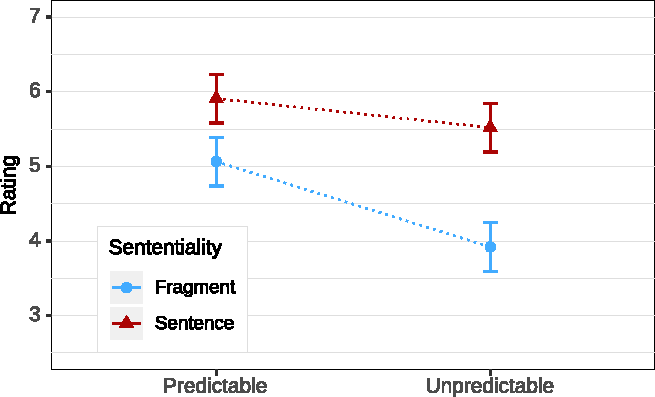
\includegraphics[scale=1]{figures/scr_rating_estimates}
 \caption{Mean ratings $+$ 95\% CIs for experiment \ref{exp:scripts-rating}. \label{fig:scripts-rating-means}}
\end{figure}

The final model contains significant main effects for both experimentally manipulated IVs. The main effect of \textsc{Sententiality} \clmmLR{30.05}{\highsig} reveals a general preference for sentences over fragments, and the main effect of \textsc{Predictability} \clmmLR{10.49}{0.01} shows that predictable utterances are also preferred overall. The significant interaction \clmmLR{9.61}{0.01} between both predictors confirms the prediction of UID\is{Uniform Information Density} that the relative preference for sentences is weaker in the predictable condition: Fragments are more acceptable when they refer to a predictable event. \textsc{ScriptKnowledge} does not seem to constrain this interaction given the model, as the three-way interaction was not significant \clmmLRnonsig{2.36}{0.1}. There is also no significant main effect of \textsc{ScriptKnowledge} \clmmLRnonsig{0.03}{0.8}, but a significant interaction with \textsc{Predictability} \clmmLR{5.08}{0.05}: The more people know about a scenario, the more they distinguish between the predictable and unpredictable conditions. The absence of any significant effect of \textsc{ScriptType} or interaction with other predictors suggests that the situational and adapted instrumental scripts\is{Script knowledge} trigger equally strong predictability effects. Finally, there is a theoretically uninteresting \textsc{Position} main effect that however does not interact with any of the other predictors and shows that ratings improve in the course of the experiment.

\begin{table}[t]
\centering
\caption{Fixed effects in the final CLMM. \label{tab:scripts-rating-estimates}}
\begin{tabular}{p{3.4cm}lllll}
\lsptoprule
Predictor & Estimate & SE & $\chi^2$ &  $p$ &  \\   
\midrule
\textsc{Sententiality}      &  -0.958 & 0.143 & 30.5 & \textless 0.001 & ***\\
\textsc{Predictability}    &   \phantom{-}0.554 &  0.162 & 10.49 & \textless 0.01 & ** \\
\textsc{ScriptKnowledge}    &  \phantom{-}0.012 &  0.109 & \phantom{1}0.03 & \phantom{\textless }0.86  &  \\
\textsc{Position}   & \phantom{-}0.021 & 0.002 & 21.57 & \textless 0.001 & *** \\
\textsc{Sententiality:}\linebreak \textsc{Predictability} &   \phantom{-}0.22 &  0.073  & \phantom{-}9.61 & \textless 0.01 & **\\
\textsc{Predictability:} \textsc{ScriptKnowledge}   &  \phantom{-}0.206 & 0.094 & \phantom{1}5.08  & \textless 0.05 & *\\
\lspbottomrule
\end{tabular}
\end{table}

\subsection{Discussion}
\label{sec:scripts-rating-discussion}
Experiment \ref{exp:scripts-rating} shows that fragments are more acceptable when they refer to a message that is predictable in context. This shows that the manipulation of utterance predictability through script knowledge\is{Script knowledge} works and that information-theoretic\is{Information theory} considerations determine the preferred form of utterances. 

\subsubsection{Script-based event chains as an approximation to context}
First of all, the experiment confirms the suitability of the script\is{Script knowledge}-based manipulation of predictability, which is empirically founded on event probabilities\is{Event chain} estimated from the DeScript corpus\is{Corpus} of script knowledge\is{Script knowledge} \citep{wanzare.etal2016}. This is evidenced by the main effect of \textsc{Predictability}, which confirms that utterances that refer to predictable events are perceived as more natural across the board. The interaction between \textsc{Predictability} and the \textsc{ScriptKnowledge} scores collected with the questionnaire following the main experiment shows that this effect is particularly strong when subjects are familiar with a scenario. This confirms the utility of the materials as triggers for script\is{Script knowledge}-based expectations.

\subsubsection{Evidence for information-theoretic constraints}

From the information-theoretic\is{Information theory} perspective, the most important result of the experiment is the significant \textsc{Sententiality:Predictability} interaction. As information theory predicts, fragments are more acceptable when they encode a predictable message than when they encode an unpredictable one. Experiment \ref{exp:scripts-rating} thus provides first empirical evidence that the perceived acceptability of a fragment depends on the likelihood of the message they encode. 

It might seem surprising that sentences were rated\is{Acceptability rating task} as more acceptable than fragments across all conditions. Fragments are frequently used, and if informa\-tion-theoretic\is{Information theory} constraints determine the choice of an utterance there must be situations where a fragment is the most well-formed encoding for a message. For most of my materials however, the sentence was also preferred in the predictable condition.%
%
\footnote{In three of the 24 items, the fragment was rated\is{Acceptability rating task} as more acceptable than the sentence in the predictable condition on average. In the unpredictable condition, this was never the case.}\afterfn%
%
Even though this is unexpected, UID\is{Uniform Information Density} does not make predictions about a main effect of \textsc{Sententiality} that could be investigated with experiment \ref{exp:scripts-rating}. UID\is{Uniform Information Density} does also not predict whether the interaction is strong enough to invert a potential preference for fragments or sentences in one of the \textsc{Predictabi\-lity} conditions, and information-theoretic constraints are certainly not the only factor that determines the choice of an encoding. Depending on which other factors are at work in the context of the relatively diverse materials, these can potentially override effects of information-theoretic constraints. Furthermore, as I anticipated above, the script knowledge\is{Script knowledge}-based predictability manipulation that I adopted implies that likely events are more likely to be talked about. Even if this assumption is correct (the production data\is{Production task} collected in experiment \ref{exp:scripts-production} confirm it), quantitative predictions about \textit{how much} more or less well-formed an encoding is can only be made if it is known how likely the corresponding message is. From this perspective, all that the experiment can show, and that it does show, is that predictability has an effect on the acceptability of fragments. Even if the likelihood of a message in the context of my materials is still unknown, the probability that a message is likely enough to license ellipsis will be higher the more likely that event is. 

\subsubsection{Why are sentences more acceptable?}

The observation that sentences are preferred over fragments both in the predictable and the unpredictable conditions is unexpected, even though as I discussed above, this does not challenge the interpretation of the data as evidence for my UID\is{Uniform Information Density}-based account. In what follows I discuss several potential reasons for this preference for sentences: (i) the written presentation modality, (ii) politeness considerations, (iii) pragmatic considerations of the choice for a specific fragment, and (iv), a potential mismatch between the likelihood of an event and that of a corresponding utterance. 

First, the written presentation might yield a preference for sentences, because fragments seem to be less appropriate in written speech. I attempted to counteract this by explicitly presenting the target utterance as spoken by one of the characters, but effects of the written presentation cannot be ruled out. Alternatively, materials could be presented auditorily, but this would increase the complexity of the experiment, because prosody must be controlled.

Second, in some situations the use of fragments might be perceived as too informal. I addressed this issue with a questionnaire on the formality of the script\is{Script knowledge}-based situation underlying my materials which was presented after experiment \ref{exp:scripts-production}. The questionnaire was presented in the same way as the script knowledge\is{Script knowledge} questionnaire presented after experiment \ref{exp:scripts-rating}. Participants used a 5-point Likert scale (5 = very formal) to rate how formal they perceived the situation described by each script\is{Script knowledge}. I then investigated a potential effect of the mean formality rating with linear models, which show that the effect of formality on the relative preference for fragments is far from being significant \lmnonsig{1}{0.26}{0.6}.%
%
\footnote{The IV in the analysis consisted in the mean formality ratings per scenario. The DV was the difference between the mean rating for the sentence and the mean rating for the fragment per scenario. The full model contained only a main effect of \textsc{Formality} and the final model was an intercept-only model. As for previous analyses, models were fit with the \texttt{lme4} package \citep{bates.etal2015} and model comparisons were conducted with the \texttt{anova} function in \texttt{R}.}\afterfn%
%
This suggests that the preference for sentences cannot be attributed to formality.

Third, the average acceptability\is{Acceptability rating task} difference between fragments and sentences might be not due to surprisingly high ratings for sentences, but because some of the fragments were not the optimal encoding in the predictive condition. Recall that in order to control the form of fragments I always tested DP\is{Determiner phrase} fragments that appeared in the postverbal position in the full sentence. This ensured that materials were as similar as possible to each other in length and internal structure, but this type of fragments is not necessarily the most optimal one with respect to UID\is{Uniform Information Density}. As I observed in the introduction to this section, fragments can have different syntactic categories, or consist of a sequence thereof. Therefore, a wide range of fragments can be derived from a single sentence like \Next[a], some of which are given in \Next[b--d]. In the specific case of the pasta scenario, the DP\is{Determiner phrase} \Next[b] might be rather uninformative\is{Shannon information}, because cooking pasta involves various events that concern the pasta. Following UID\is{Uniform Information Density}, in this case, \textit{the pasta} might be omitted due to its predictability rather than the PP\is{Preposition phrase} in \Next[d], which would survive ellipsis because it is less predictable. If that was the case, at least some of the fragments tested in the experiment might not (only) be degraded because a sentence is preferred in the situation, but because there are other fragments that are more well-formed and can communicate the same message.

\ex. \a. Pour the pasta into the pot, please!
\b. The pasta!
\c. The pasta into the pot!
\d. Into the pot!

Finally, the assumption underlying the design of the materials, that a likely event is more likely to be talked about, so far has not been empirically evidenced. As I noted above, information theory\is{Information theory} might even predict the opposite, because referring to an event that follows necessarily from context is extremely redundant.%
%
\footnote{Such considerations also seem to be reflected in the original DeScript data. Some contributors to the corpus\is{Corpus} provide very brief descriptions of the cooking pasta scenario, for instance they omit events like pouring salt into the water or even the action of turning the stove on, which is a necessary condition for events that occur later in the script\is{Script knowledge}.}\afterfn%
%
If the messages in the predictable conditions were not as likely as I assumed them to be, this would also explain the overall preference for sentences. This does not undermine the conclusions that I draw so far from the experiment: If utterances that refer to predictable events were unlikely in the context of my materials, the interaction would be expected to go in the opposite direction. Even if both the fragment and the sentence were highly redundant, UID\is{Uniform Information Density} still predicts that the less redundant fragment will be preferred over the full sentence.%
%
\footnote{\citet{schafer.etalunderreview} present data on verb phrase ellipsis\is{Verb phrase ellipsis} that are in line with this prediction. In a self-paced reading experiment, they find that longer redundant VPs\is{Verb phrase} \Next[a] are read faster than shorter ones \Next[b] (per word). This indicates lower average surprisal\is{Shannon information} on the longer VPs\is{Verb phrase}. Rating data show that realization of the redundant VP\is{Verb phrase} is more degraded in the long condition than in the short one.

\ex. \a. John played football, and Bill \textit{played football}, too.
    \b.  John played football in the backyard of the house, and Bill \textit{played football in the backyard of the house}, too.

}\afterfn%
% 
This calls for an empirical estimation of the message probability in my materials, which is one of the goals of experiment \ref{exp:scripts-production}. Anticipating the results that I discuss in greater detail in Section \ref{sec:scripts-production-results-check}, the message underlying my materials in the predictable condition is indeed more likely (19.1\%) than that in the unpredictable condition (0.4\%). However, there is a large degree of variation between items. For instance, in the train scenario the message used in the predictable condition was produced in 96.6\% of the trials, whereas there were three scenarios for which the target utterance tested in the predictable condition was never produced.

\subsubsection{Summary and outlook}
Taken together, experiment \ref{exp:scripts-rating} shows that fragments are more acceptable when they refer to a message that is predictable in context. This supports my hypothesis that predictable utterances are more likely to be reduced. The overall preference for sentences is unexpected but does not contradict the predictions of information\is{Shannon information} theory. However, this finding is expected both under UID\is{Uniform Information Density} and a source coding\is{Source coding} approach, which predicts a general tendency to assign shorter codes to more likely messages. UID\is{Uniform Information Density} additionally predicts that specifically those words that are more predictable are omitted. This is investigated with a production task\is{Production task} in experiment \ref{exp:scripts-production}. The production data will also show whether the messages tested in the predictable condition are indeed likely more likely than the presumably unpredictable ones.

%%%%%%%%%%%%%%%%%%%%%%%%%%%%%%%%%%%%%%%%%%%%%%%%%%%%%%%
%%%%%%%%%%%%%%%%%% SKRIPTWISSEN PRODUKTION %%%%%%%%%%%%
%%%%%%%%%%%%%%%%%%%%%%%%%%%%%%%%%%%%%%%%%%%%%%%%%%%%%%%
\refstepcounter{expcounter}\label{exp:scripts-production}
\section{Experiment \ref{exp:scripts-production}: Script knowledge, production}  \label{sec:scripts-production}
\subsection{Background}
\label{sec:scripts-production-background}

Experiment \ref{exp:scripts-rating} showed that fragments are relatively more acceptable when they encode predictable messages. Even though this follows from UID\is{Uniform Information Density}, it is also predicted by a source coding\is{Source coding} account that simply assigns shorter codes to more likely messages. Experiment \ref{exp:scripts-production} investigates the two more fine-grained predictions of UID\is{Uniform Information Density} on the word level: First, predictable words are more likely to be omitted, because this avoids troughs in the ID profile\is{Information density}. Second, words that reduce the surprisal\is{Shannon information} of unpredictable following words are more likely to be realized, since this smooths peaks in the ID profile\is{Information density}. Source coding\is{Source coding} predicts an overall densification strategy for predictable utterances, but only UID\is{Uniform Information Density} predicts \textit{which} words are omitted and that channel capacity\is{Channel capacity} limits the densification of utterances. This upper bound will be specifically evidenced by the insertion of redundant material in order to reduce peaks in the ID profile\is{Information density}, which is not predicted by source coding\is{Source coding}.

Investigating these predictions empirically requires (i) a data set that contains such omissions, (ii) to know  which words have been omitted, and (iii) a method to estimate information\is{Shannon information} in the presence of omissions. Following the approach taken by \citet{levy.jaeger2007} and subsequent work, logistic regressions can then be used to test whether information\is{Shannon information}-theoretic\is{Information theory} measures significantly contribute to predicting whether this word has been omitted or not in the data set. In experiment \ref{exp:scripts-production} I collected such a data set with a production tsk using the same stimuli as in experiment \ref{exp:scripts-rating}, which contains about 100 utterances for each of the script-based\is{Script knowledge} stories. This allows me to quantify the likelihood of utterances in the extralinguistic context\is{Context, extralinguistic} modeled by the stories. The data were preprocessed so that omissions can be unambiguously reconstructed. I estimate word probabilities for omitted and realized words in this data set with  a new method of surprisal\is{Shannon information} estimation which is not confounded by omissions in the data.

Experiment \ref{exp:scripts-production} will also provide further insights on the question of whether word order\is{Word order} variation is driven by UID\is{Uniform Information Density}. As I discussed in Section \ref{sec:infotheory-uid}, it has been argued in the literature that the average surprisal\is{Shannon information} of words is lower the more material precedes them in the clause. Therefore, placing unpredictable words in a sentence-final position and predictable ones sentence-initially yields a more uniform ID profile\is{Information density} on average. Finally, the experiment will show whether the utterances in the predictable condition of the rating study\is{Acceptability rating task} were indeed more likely than the unpredictable ones. As I observed in the discussion of experiment \ref{exp:scripts-rating}, likely events are not necessarily likely to be talked about, because the corresponding utterances are rather uninformative\is{Shannon information}.

\subsection{Materials}
I used the context stories of experiment \ref{exp:scripts-rating} as stimuli. These stories consist of four sentences, the first one introduces the script\is{Script knowledge} and the other three ones describe a sequence of three events\is{Event chain} that are likely to follow each other in DeScript. The stimulus corresponding to the pasta script\is{Script knowledge} is given in \Next.%
%
\footnote{I provide English\il{English} translations of the materials in this section, but the experiment was done in German\il{German}.}\afterfn%
% 
In the rating study\is{Acceptability rating task}, the sentence introducing the utterance was always a complete sentence, e.g. \textit{Now Annika says to Jenny}. In the production study\is{Production task} this sentence was replaced by a fragment of the form \textit{$\langle$Person A$\rangle$ to $\langle$Person B$\rangle$}. Otherwise the force of this introduction could have biased participants to produce e.g. declarative or interrogative utterances instead of the overall most likely utterance.

\ex. Annika and Jenny want to cook pasta. Annika put a pot with water on the stove. Then she turned the stove on. After a few minutes, the water started to boil. \\Annika to Jenny: \label{ex:scripts-production-item}

I collected data for the 24 scripts\is{Script knowledge} on which the materials in experiment \ref{exp:scripts-rating} were based. Some of the materials were slightly adapted, so that there were only two characters in each script\is{Script knowledge}. In the rating study\is{Acceptability rating task}, some stories had three participants, for instance, the traveling couple and an airline employee. %

\subsection{Procedure}
The experiment was completed by 198 self-reported native speakers of German\il{German}, who were recruited for the experiment on the \textit{clickworker} crowdsourcing platform. Subjects were paid \currencyEuro{2} for participating in the study. The task consisted in reading the context story and entering the sentence the subject considered most likely into a text field. Initially, I planned to collect two data sets using the same materials, one that contains omissions and one that contains only complete sentences. The nonelliptical data set could then be used for surprisal\is{Shannon information} estimation (without surprisal\is{Shannon information} being affected by omissions) whereas the data set containing omissions would have shown whether word probabilities in the nonelliptical data set predict the actual distribution of omissions. However, even though participants were instructed to produce \textit{complete sentences}, they produced a relatively high ratio of utterances containing omissions. Therefore, I used this data set as the elliptical one and reconstructed ellipses as described in Section \ref{sec:scripts-production-annotation} in order to obtain a nonelliptical data set for probability estimation. In order to rule out the possibility that the term \textit{sentence} in the instructions resulted in an artificially low rate of omissions, I collected a smaller data set ($n$ = 30 for each script) replacing the term \textit{sentence} in the instructions by \textit{utterance}. I then compared the ratio of elliptical utterances, which lacked at least one word that appears obligatorily in a full sentence between both data sets. In the data set collected by asking for \textit{utterances}, the rate of elliptical utterances (25.74\%) was slightly higher than in the data set collected by asking for \textit{sentences} (23.79\%). A linear mixed effects regression on the item level shows that this difference is not significant \clmmLRnonsig{0.8}{0.37}. I conclude that the term \textit{sentence} in the instructions did not bias subjects' behavior as compared to \textit{utterance} and therefore used the larger data set for analysis and reconstructed the nonelliptical data set for analysis.

Subjects were also told that they would read statements like \textit{$\langle$Person A$\rangle$ to $\langle$Person B$\rangle$} after the story, and that these statements specified whose utterance they should produce. Subjects were assigned to one of two lists, and each list was worked on by 99 participants. Each list contained half of the 24 script-based\is{Script knowledge} materials and eigtht further stimuli. These materials had the same form as the script-based\is{Script knowledge} materials (a four-sentence context story), required the same task and also described potentially script-based\is{Script knowledge} situations. However, they were not as based on empirically measured event probabilities. The purpose of including them was to obtain a larger data base for future analyses of omissions in fragments. Materials were presented in fully randomized order. After data collection, subjects were asked to complete a questionnaire on how formal they perceived the situations described in the materials on a 5-point Likert scale (5 = very formal). These data were used as predictor for the post-hoc analysis on formality in the rating study\is{Acceptability rating task} that I reported in the discussion of experiment \ref{sec:scripts-rating}. There were no attention checks, but the data provided by some subjects were excluded because they entered random character strings or copied part of the stimulus into the text field.

\subsection{Preprocessing} \label{sec:scripts-production-annotation}

The raw data set comprised about 100 utterances for each of the 24 items. Subjects produced a diverse set of utterances even for semantically identical or very similar meanings referring to the same event. \Next shows some typical responses for the pasta script\is{Script knowledge}. For instance, the responses vary with respect to lexical alternatives such as the synonyms \textit{Pasta} and \textit{Nudeln} in \Next[a,b], optional adverbials\is{Adverbial} like \textit{jetzt} `now' in \Next[c] and omissions like that of \textit{in den Topf} `into the pot' in \Next[d]. In addition, these utterances vary in word order\is{Word order}, which depends on the insertion of modals as \textit{kannst} `can' in \Next[a--c] that make the indirect speech act more polite and on sentence force, as the difference between declaratives and interrogatives in \Last[c,d] shows.

\ex. \ag. Kannst du die Pasta in den Topf tun?\\
can.\textsc{2sg} you the pasta in the.\textsc{acc} pot do\\
\trans{Can you put the pasta into the pot?}
\bg. Kannst du die Nudeln in den Topf füllen?\\
can.\textsc{2sg} you the noodles in the.\textsc{acc} pot fill\\
\trans{Can you put the pasta into the pot?}
\cg. Wir können jetzt die Nudeln rein tun.\\
we can now the pasta inside do\\
\trans{Now we can put the pasta in.}
\dg. Gibst du die Nudeln rein?\\
give.\textsc{2sg} you the noodles inside\\
\trans{Can you put the pasta in?}

The diversity in the production data\is{Production task} results in two problems that were addressed by preprocessing the data to a standardized form. First, it complicates the resolution of ellipsis, which is necessary in order to investigate whether those words that have been omitted are really more predictable than those which are realized. If there are two synonym lexical alternatives like \textit{Nudeln} and \textit{Pasta}, even if it is obvious that a word referring to \textit{the pasta} is missing, it is unclear which of the alternatives is to be inserted. Second, language models operate on word forms and treat synonyms like \textit{Nudeln} and \textit{Pasta} as distinct expressions. However, if a DP\is{Determiner phrase} referring to the pasta is omitted because of its high predictability, this should be reflected in the information\is{Shannon information} estimated by the language model instead of splitting its probability mass between various synonyms.%
%
\footnote{Higher order \textit{n}-grams\is{N-gram language model} boost this problem further. For instance, only two synonym verbs \textit{reingeben}, \textit{reintun} (`to put inside') and two synonym words for the pasta split the probability mass of \textit{pour pasta} across four bigrams\is{Bigram language model}.}\afterfn%
%

\begin{figure}[t]
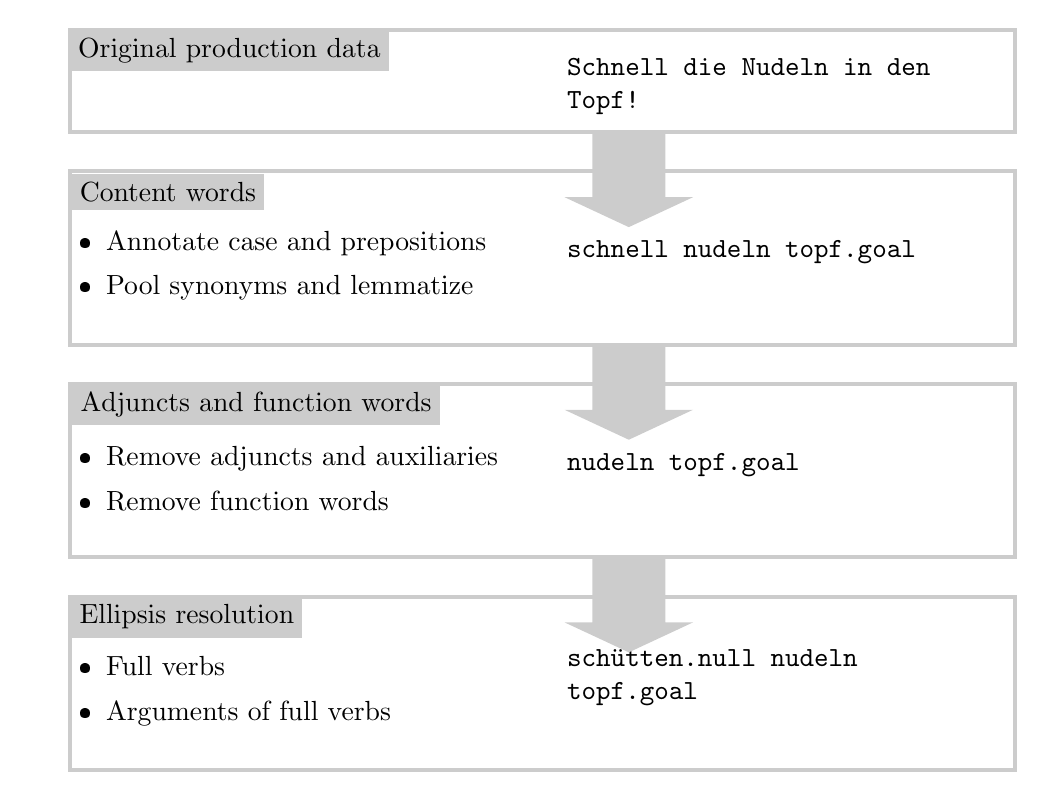
\begin{tikzpicture}[scale=1]
\draw [draw = black!20!, line width = .5mm] (0,-.9) rectangle (12,-2.2);
\node (t) at (2.026,-1.16) [fill = black!20!, inner sep = 3pt] {Original production data};
\node (mp) at (5.7,-2){
\begin{minipage}{6cm}
~~
\end{minipage}
\begin{minipage}{.5cm}
 ~~
\end{minipage}
\begin{minipage}{5.5cm}
\texttt{Schnell die Nudeln in den Topf!}\\
\vspace{.4cm}
\end{minipage}

};
%%% CONTENT EXTRACTION
\draw [draw = black!20!, line width = .5mm] (0,-2.7) rectangle (12,-4.9);
\node (t) at (1.247,-2.96) [fill = black!20!, inner sep = 3pt] {Content words};
\node (mp) at (5.7,-4.1){
\begin{minipage}{6cm}
\vspace{-.4cm}
\begin{itemize} \itemsep0em
  \item Annotate  case and prepositions 
 \item Pool synonyms and lemmatize
\end{itemize}
\end{minipage}
\begin{minipage}{.5cm}
 ~~
\end{minipage}
\begin{minipage}{5.5cm}
\texttt{schnell nudeln topf.goal}\\
\vspace{.4cm}
\end{minipage}

};

\draw [draw = black!20!, line width = .5mm] (0,-5.4) rectangle (12,-7.6);
\node (t) at (2.367,-5.66) [fill = black!20!, inner sep = 3pt] {Adjuncts and function words};
\node (mp) at (5.7,-6.8){
\begin{minipage}{6cm}
\vspace{-.4cm}
 \begin{itemize} \itemsep0em
  \item Remove adjuncts and auxiliaries
  \item Remove function words
\end{itemize}
\end{minipage}
\begin{minipage}{.5cm}
 ~~
\end{minipage}
\begin{minipage}{5.5cm}
\texttt{nudeln topf.goal}\\
\vspace{.4cm}
\end{minipage}

};

\draw [draw = black!20!, line width = .5mm] (0,-8.1) rectangle (12,-10.3);
\node (t) at (1.487,-8.36) [fill = black!20!, inner sep = 3pt] {Ellipsis resolution};
\node (mp) at (5.7,-9.5){
\begin{minipage}{6cm}
\vspace{-.4cm}
 \begin{itemize} \itemsep0em
  \item Full verbs
  \item Arguments of full verbs
\end{itemize}
\end{minipage}
\begin{minipage}{.5cm}
 ~~
\end{minipage}
\begin{minipage}{5.5cm}
\texttt{schütten.null nudeln topf.goal}\\
\vspace{.4cm}
\end{minipage}

};
\node at (7.1,-2.7)[single arrow, single arrow head extend=10pt, single arrow tip angle=130, shape border rotate=270,inner sep=8pt, fill=black!20!, minimum height=1.2cm]{~~~~};
\node at (7.1,-5.4)[single arrow, single arrow head extend=10pt, single arrow tip angle=130, shape border rotate=270,inner sep=8pt, fill=black!20!, minimum height=1.2cm]{~~~~};
\node at (7.1,-8.1)[single arrow, single arrow head extend=10pt, single arrow tip angle=130, shape border rotate=270,inner sep=8pt, fill=black!20!, minimum height=1.2cm]{~~~~};

\end{tikzpicture}
\caption{Overview of the preprocessing procedure applied to the production data. First, case and prepositions are annotated on the noun phrases, then the adverb \textit{schnell} is removed and finally the missing verb \textit{schütten} (`to pour') reconstructed.\label{fig:prod-preprocessing}}
\end{figure}
%
Therefore, all utterances produced by the subjects were manually annotated according to a procedure, which is exemplified in Figure \ref{fig:prod-preprocessing} and which transforms an utterance like \Next[a] into an abstract representation \Next[b]. Overall, preprocessing consisted in a trade-off between the necessary standardization and the preservation of as much variation in the original data as possible. Specifically, preprocessing preserved word order\is{Word order} and morphosyntactic properties of noun phrases\is{Noun phrase}, such as distinctive case inflections, which provide a cue toward the \texttheta-role of the noun in fragments. The standardization consisted in pooling synonyms and removing adjuncts\is{Adjunct}, adverbials\is{Adverbial} and function words. Finally, I also annotated representations of the meaning of each utterance. This annotation layer is necessary to investigate whether more predictable meanings are assigned shorter codes and to relate the production data\is{Production task} to the rating data\is{Acceptability rating task} from experiment \ref{exp:scripts-rating}.

\ex. \ag. Schnell die Nudeln in den Topf!\\
	  quickly the pasta in the pot\\
	  \trans{(Pour) the pasta quickly into the pot!}
     \bg. \texttt{schütten.\textsc{null}} \texttt{nudeln} \texttt{topf.\textsc{goal}}\\
	pour.\textsc{null} pasta pot.\textsc{goal}\\

\subsubsection{Exclusion of noisy data}
Before preprocessing, data that were clearly not meaningful utterances in the situation described in the stimulus were removed from the data set. This concerns data from two subjects who provided responses in English\il{English}, responses consisting in random character strings, copied and pasted parts of the stimulus material or nonsense utterances. For instance, one subject repeatedly entered `hello', even in scripts\is{Script knowledge} where it was unnatural that one of the characters would greet the other one. Utterances that corresponded to wrong turns (e.g. by the customer in the library script, where subjects were asked to provide an utterance by the librarian) were also excluded. This resulted in a loss of 8.82\% of the responses. Sometimes subjects provided two or more utterances in a single trial, such as the example in \Next. In such cases, both utterances were separated and treated as individual utterances by the same subject. Separation occurred when two matrix sentences were separated by punctuation characters.

\exg. Gibst du mir bitte die Nudeln? Das Wasser kocht.\\
      give.\textsc{2sg} you me.\textsc{dat} please the noodles the water boils\\
      \trans{Would you give me the pasta, please? The water is boiling.}

\subsubsection{Annotation of content words}

All utterances were transformed into representations that contain the matrix verb and its arguments. In the complete data from a script, i.e. item, all coreferent nouns were pooled to the same lemma, for instance \textit{Pasta} and \textit{Nudeln} were merged to \texttt{nudeln}. Among the synonyms, the most frequent one was chosen as a label. The same procedure was applied to synonym verbs, such as \textit{schütten} `pour', \textit{füllen} `fill', \textit{reingeben} `put inside' and \textit{reintun} `put inside' in \LLast, which were merged to \texttt{schütten} `pour'. Some verbs are ambiguous, for instance, \textit{geben} can be used either as a part of a particle verb \textit{reingeben} `put inside', like in \LLast[d], but it can also describe a transfer of possession `give' as in \Last. Therefore, only the instances of \textit{geben} belonging to the particle verb were pooled to \texttt{schütten}. Pronouns were also resolved and pooled to the corresponding noun lemma.

For all nouns, distinctive case morphology was annotated as a suffix $.\langle$\textsc{case}$\rangle$ attached to the noun to ensure that the language model treated nouns with differential case marking (but only those) as different items. This is relevant because experiments \ref{exp:case}--\ref{exp:scripts-rating-case} provided evidence for case connectivity\is{Case connectivity}: A DP\is{Determiner phrase} fragment appears in the same case as the DP\is{Determiner phrase} in the corresponding full sentence does. From the hearer's perspective, case can thus be a strong cue toward a specific complete sentence. For instance, a dative\is{Dative case} DP\is{Determiner phrase} fragment excludes all possible interpretations that require it to appear in accusative\is{Accusative case}. Case was annotated only when it was morphologically distinguished, because otherwise it does not function as such a cue. Similarly, prepositions were annotated as a suffix $.\langle$\textsc{preposition}$\rangle$ attached to the noun, because the experiments on preposition omission\is{Preposition omission} in German\il{German} showed that there is a strong tendency not to omit prepositions\is{Preposition omission} in PPs\is{Preposition phrase} in German\il{German}.

\subsubsection{Removal of function words, adverbials and auxiliaries}
After the annotation of case and preposition information on nouns, all function words, like articles and prepositions, modal verbs and auxiliaries as well as optional words like adjuncts\is{Adjunct} were removed from the data set. As for function words, the reason for this is that articles\is{Article omission} and prepositions\is{Preposition omission} cannot be freely omitted in German\il{German}: Article omission\is{Article omission} is not grammatical in standard German\il{German} but only in specific text types \citep{reich2011, reich2017}, and my experiment \ref{exp:pstranding-german} showed that the omission of prepositions\is{Preposition omission} is heavily degraded. Since the purpose of collecting this data set is to investigate omissions on the word level, treating e.g. a preposition\is{Preposition phrase} and its complement DP\is{Determiner phrase} as two separate units would falsely suggest that they can be omitted independently from each other. Adverbials\is{Adverbial} can be inserted relatively freely at various positions of the sentence in German\il{German} \citep[209]{eisenberg1999}, but often the information\is{Shannon information} that they convey, such as time, place or manner is left implicit. Therefore, it is not reasonable to assume that e.g. \Next involves ellipsis of a temporal and a locative adverbial \citep[1850]{reich2011}. 

\ex. $\langle$Yesterday evening$\rangle$ John ate a pizza $\langle$at Giordano's$\rangle$.

Of course, the aspects of meaning contributed by adverbials\is{Adverbial} might be also subject to UID\is{Uniform Information Density}: If John eats at Giordano's frequently, the adverbial \textit{at Giordano's} will be less informative\is{Shannon information} and therefore more likely to be omitted than if he does only rarely. However, omitting the adverbial does not yield a fragment under any theoretical account, therefore the omission of such optional expressions is not directly relevant to my research questions.

Modal verbs and auxiliaries can affect word order\is{Word order} in German\il{German}. Specifically in questions which are used as indirect speech acts, the modal verb occurs in the sentence-initial matrix verb position and the main verb utterance-finally \Next[a]. In declaratives, modals occupy the default left bracket position \Next[b]. In order to keep the annotation procedure simple I omitted any occurring modals, but left the main verb in the final position where it appears in the original data. Maintaining the original word order\is{Word order} as much as possible is necessary in order to take into account effects of word order\is{Word order} on information\is{Shannon information}. Utterance-final words can be predicted from preceding material \citep{levy2008}%
%
\footnote{But see \citet{balling.kizach2017} for conflicting results on Danish\il{Danish}.}\afterfn%
%
and will therefore be on average less informative\is{Shannon information} than sentence-initial ones.

\ex. \ag. Kannst du die Nudeln in den Topf füllen?\\
can.\textsc{2sg} you the noodles in the.\textsc{acc} pot fill\\
\trans{Could you fill the pasta into the pot?}
\bg. Du könntest schon mal die Teller auf den Tisch stellen.\\
you can.\textsc{sbjv.2sg} already \textsc{prt} the plates on the table put\\
\trans{You could now put the plates on the table.}

\subsubsection{Ellipsis resolution}

In order to estimate (and to later compare) the surprisal\is{Shannon information} of realized and originally omitted words, all ellipses, i.e. omissions of words that are obligatory in full sentences, were reconstructed. This involved specifically the insertion of omitted main verbs and arguments. Note that the set of ellipses in the data encompasses not only those omissions that yield fragments according to the definition provided in Section \ref{sec:intro-fragments}, but also argument omissions. Testing whether omissions of individual words are in line with the predictions of UID\is{Uniform Information Density} requires not only to compare fragments and complete sentences, but to take into account also the possibility of other argument ellipses, like topic\is{Topic drop} or object drop\is{Object drop}.

\begin{sloppypar}
Ellipses could in general be unambiguously resolved, because the reconstruction procedure operated on the preprocessed simplified representations described above and there were no lexical alternatives to choose from. If there were several possibilities of enriching a fragment, the strategy that required the least amount of insertions and default subject-initial word order\is{Word order} was pursued. All words inserted during this procedure received an additional tag \texttt{.NULL}, which indicated that they had been omitted in the utterances produced by the subjects. The purpose of the tag was to keep track of which words had been omitted and which ones had been realized in the original data set. In the statistical analysis, I used this binary \textsc{Omission} predictor as the dependent variable.
\end{sloppypar}

Based on the annotated data, I created two versions of the data set: The \textit{original} data set, where I kept track of actual omissions, and the \textit{enriched} data set, which was used only for the purpose of surprisal\is{Shannon information} estimation. This data set contains all of the originally produced words and those that had been inserted through ellipsis reconstruction. I removed the \texttt{.NULL} tags assigned to reconstructed words from the words in this data set, since otherwise the reconstructed and realized occurrences of the same word would be treated as different lexicon entries during surprisal\is{Shannon information} calculation. Using a data set without omissions for surprisal\is{Shannon information} estimation addresses a central problem of language modeling on elliptical data: If UID\is{Uniform Information Density} is correct, word probabilities estimated from a regular corpus\is{Corpus} are not proportional to the likelihood of these words. Since speakers omit predictable words more often, they are expected to be rare in the corpus\is{Corpus}, or at least not as frequent as they would be without omissions. Therefore, word probabilities estimated from a regular corpus\is{Corpus} are not proportional to the likelihood of these words. This circularity issue, which is discussed in detail below in Section \ref{sec:scripts-production-surprisal-context}, does not arise in data sets which do not contain any omissions.

\subsubsection{Annotation of messages}
Finally, the meaning of each utterance was annotated as a simplified semantic representation consisting of a verb and its arguments. These representations were formally identical to those in the enriched data set, but insensitive to word order\is{Word order}. The rationale was to assign the same single label to all meaning-equivalent expressions. The purpose of this annotation layer was to be able to quantify the likelihood of meanings and to model the mapping from signals (i.e., utterances) to messages. In this case this mapping was unidirectional, so that various signals could refer to the same message, but not \textit{vice versa}. In principle the opposite would also be possible, but there were no ambiguous utterances in the context of the tightly constrained script-based\is{Script knowledge} stories. 

\subsection{Surprisal estimation}
\label{sec:scripts-production-surprisal}

I argued above that reasonably estimating the surprisal\is{Shannon information} of words in fragments is possible as long as effects of extralinguistic context\is{Context, extralinguistic} can be taken into account and it is known which words have been omitted. The data set whose collection and preprocessing is described in the preceding section conforms to both of these needs. The contexts\is{Context, extralinguistic} used for data elicitation ensure that the probabilities of words and utterances in the data set are conditioned on these contexts. The reconstruction of ellipsis solves the circularity issue that might arise from the frequent omission of predictable words: Surprisal can be estimated from the enriched data, which includes words that have originally been omitted and is consequently not increased by their more frequent omission.

I explore effects of three information-theoretic\is{Information theory} predictors on omissions. In order to take the script-based\is{Script knowledge} approximation to extralinguistic context\is{Context, extralinguistic} into account, I apply all methods separately to the data for each script\is{Script knowledge}. The first method that I use is simply unigram\is{Unigram language model} surprisal\is{Shannon information}. Since the language models are trained on the data for each script\is{Script knowledge} separately, unigram\is{Unigram language model} surprisal\is{Shannon information} models extralinguistic context\is{Context, extralinguistic}. This contrasts with unigram\is{Unigram language model} surprisal\is{Shannon information} estimated from larger and more balanced corpora\is{Corpus}, where the frequency of a word is not conditional on a tightly controlled context. The second method that is an extension of the calculation of surprisal\is{Shannon information} suggested by \citet{hale2001}. In addition to extralinguistic context\is{Context, extralinguistic}, this method also takes linguistic context\is{Context, linguistic} into account, and unlike \citeauthor{hale2001}'s original method, it can deal with the possibility of arbitrary omissions in fragments. These two surprisal\is{Shannon information} measures will show whether predictable words are more likely to be omitted. I interpret this as the result of a strategy to avoid troughs in the ID profile\is{Information density}. Finally, I use a measure of surprisal\is{Shannon information} reduction, which is technically similar to context-dependent surprisal\is{Shannon information}, in order to investigate to what extent non-final words reduce the surprisal\is{Shannon information} of the following word. This could provide evidence for a strategy to avoid peaks in the ID profile\is{Information density}.

\subsubsection{Unigram surprisal}

Unigram language models\is{Unigram language model} with Good-Turing discount were trained on the enriched data ($n \sim 100$) for each script\is{Script knowledge} using the SRILM toolkit \citep{stolcke2002}. I estimated unigram surprisal\is{Shannon information} for each script\is{Script knowledge} independently. This method allows for the interpretation of the probability estimate $S(w_i) = -\log_2 p(w_i)$ for a word $w_i$ as the probability of $w_i$  given extralinguistic context\is{Context, extralinguistic}, which is set by the context story, i.e. $S(w_i) = -\log_2 p(w_i\mathbin{|} context_{extraling.})$. The by-word unigram surprisal\is{Shannon information} values were then extracted from the language model files and annotated with Python scripts for each word in the production data. 

\subsubsection{Taking linguistic context into account}
\label{sec:scripts-production-surprisal-context}

In previous studies on predictability effects on linguistic encoding preferences, the probability of words in context has been estimated with \textit{n}-gram language models\is{N-gram language model}. As I anticipated above, training \textit{n}-gram models on corpora that contain elliptical data results in a circularity issue: If predictable words are more often omitted, they will appear to be rare in the corpus\is{Corpus} just because of their expected high rate of predictability-driven omission. 

In the case of unigram\is{Unigram language model} surprisal\is{Shannon information}, this issue can be addressed by training the models on the enriched data set, where all ellipses have been reconstructed. Since there are no omissions in the data, all surprisal\is{Shannon information} estimates reflect the true probability of a target word. However, training higher order \textit{n}-grams\is{N-gram language model} on the enriched data set would result in a further issue, because now words that have been originally omitted would be included in the context of a target word and consequently modulate its probability. This is of course highly implausible, because omitted words are not available to the hearer and therefore cannot contribute to this probability. For instance, if somebody uttered the fragment \Next[a] in the pasta scenario, the corresponding structure in the enriched data set would be \Next[b]. A regular bigram model\is{Bigram language model} trained on the enriched data estimates the surprisal\is{Shannon information} of the DP\is{Determiner phrase} fragment as $S_{pasta} = -\log_2 p(pasta\mathbin{|}pour)$. If the verb increases the likelihood of objects that can be poured in this context\is{Context, linguistic}, the surprisal\is{Shannon information} of pasta would be underestimated in comparison to its true value in a discourse-initial\is{Fragment, discourse-initial} fragment like \Next[a].%
%
\footnote{In the literature on grammatical function words, studies investigating effects of a function word's predictability on its own omission (avoid troughs) have used the likelihood of the construction marked by the function word, like a relative  or complement clause\is{Complement clause}, as an approximation to the function word's surprisal\is{Shannon information} \citep{levy.jaeger2007, jaeger2010}. In an analysis investigating whether redundant relative pronouns are inserted before unpredictable target words, \citet{levy.jaeger2007} train their models on a modified version of the corpus\is{Corpus}, from which all relative pronouns have been removed. Therefore, relative pronoun omissions do not affect the estimated surprisal\is{Shannon information} of the target word. Obviously both approaches cannot be applied to fragments, because omissions can target any word in my preprocessed data set.}\afterfn%
%

\ex. \a. The pasta, please!  \label{ex:scripts-production-hale-frag}
     \b. \texttt{pour} \texttt{pasta} \texttt{pot.GOAL} \label{ex:scripts-production-hale-act}

Therefore, I estimated surprisal\is{Shannon information} with a method based on the approach suggested by \citet{hale2001}. \citeauthor{hale2001} derives surprisal\is{Shannon information} from a parallel parser\is{Parser, parallel}\is{Parser, human} that computes all possible parses and rejects those parses that are incompatible with the current input. The set of possible parses is correspondingly updated after processing each word. One of \citeauthor{hale2001}'s main insights is that the amount of work done by the parser\is{Parser, human} is proportional to the total probability mass of the rejected parses: The higher this probability mass is, the more informative\is{Shannon information} is a word.

\is{Parser, parallel|(}This method requires knowing (i) which parses are possible in a situation and (ii) how likely each parse is. \citet{hale2001} obtains both of these measures from a probabilistic context-free grammar (PCFG\is{Context-free grammar}), which comprises a set of re-write rules whose likelihood can be estimated from a corpus\is{Corpus}. The likelihood of a parse is calculated as the product of the probabilities of the individual rules that are required to generate that parse.\is{Parser, parallel|)} Instead of using PCFG\is{Context-free grammar}s, I assume that my enriched production data\is{Production task} set shows which complete structures are possible in that situation and how likely they are. This approach restricts the set of possible parses to those that actually have been produced and therefore excludes pragmatically odd ones, like \Next. In contrast, a PCFG\is{Context-free grammar} does not exclude odd utterances if they can be derived by its rules. If there is a rule \NNext[a] in the PCFG\is{Context-free grammar}, the unlikely \Next and the likely \Last[b] differ only in the likelihood of the two rules in \NNext, because the other rules required to generate both utterances are identical. Therefore, a PCFG\is{Context-free grammar} could assign a relatively high probability to utterances that are unexpected for pragmatic reasons as compared to a human hearer, who would not expect a request to pour the salt on the table. It seems more psychologically realistic to assume that when a speaker parses\is{Parser, human} the word \textit{pour} and \textit{salt}, the likelihood of \texttt{table.GOAL} as compared to \texttt{pot.GOAL} is not only subject to the likelihood of the re-write rules in \NNext but to a particular context for which a PCFG\is{Context-free grammar} does not account. 

\ex. \texttt{pour} \texttt{salt} \texttt{table.GOAL}

\ex. \a. PP\is{Preposition phrase} $\rightarrow$ \texttt{table.GOAL}
     \b. PP\is{Preposition phrase} $\rightarrow$ \texttt{pot.GOAL}

Therefore, I take the set of unique produced utterances in the enriched data set to represent the range of possible structures and their frequency in the data set to reflect their likelihood in the context of the story. For instance, the German\il{German} equivalent to \ref{ex:scripts-production-hale-act} occurs 16 times among the 115 utterances of the pasta data set, so its likelihood is 0.139. Note that this figure does not represent the likelihood of a sentence equivalent to \ref{ex:scripts-production-hale-act} to be actually produced, because it has been calculated based on the enriched data set and not based on the original production data\is{Production task} that contain omissions, but the likelihood of an utterance that, if it is enriched, corresponds to this representation. Knowing the range of possible structures and their respective probabilities is necessary for the estimation of by-word information\is{Shannon information}.

\is{Parser, parallel|(}Given this general setup, \citet{hale2001} defines surprisal\is{Shannon information} as the logarithm of the ratio of the prefix probability \textalpha, i.e. the probability mass of the parses that are compatible with an input \textit{before} parsing that word to the probability mass of the parses that remain active \textit{after} processing it:

\begin{equation}
 \displaystyle S(w_n) = \log_2 \frac{\alpha_{n-1}}{\alpha_n}
\end{equation}

This measure increases the more $w_i$ narrows the set of parses that are compatible with the input as compared to $\alpha_{n-1}$. If $w_i$ is compatible with all parses that $w_{i-1}$ is compatible with, it equals 0. In the case of utterance-initial words, surprisal\is{Shannon information} is thus equivalent to the negative logarithm of the cumulated probability of all parses (that is, enriched complete structures) that begin with this word.  For illustration, consider the case of an utterance like \Next[a] in the artificial example in \Next, where there are only the four parses in \Next[a--d].

\ex. \label{ex:contexts-pd} \a. \texttt{pour} \texttt{pasta} \texttt{pot.GOAL} \hfill $p = 0.75$\label{ex:contexts-a}
 \b. \texttt{pour} \texttt{salt} \texttt{pot.GOAL} \hfill $p = 0.2$\label{ex:contexts-b}
 \c. \texttt{set} \texttt{table} \hfill $p = 0.03$\label{ex:contexts-c}
 \d. \texttt{pour} \texttt{sauce} \texttt{pan.GOAL}\hfill  $p = 0.02$\label{ex:contexts-d}
 
In this situation, processing \texttt{pour} excludes only the parse in \Last[c], so that $\alpha_{n} = 0.97$. The prefix probability before parsing \texttt{pour}, $\alpha_{n-1} = 1$, because before processing any input no parse is excluded. The surprisal\is{Shannon information} of \texttt{pour} is thus calculated as shown in Equation \ref{eq:surprisal-pour}.

\begin{equation}
 \displaystyle S(pour) = \log_2 \frac{1}{0.97} = 0.04 \label{eq:surprisal-pour}
\end{equation}

The surprisal\is{Shannon information} of \textit{pasta} after processing \textit{pour} is calculated as shown in Equation \ref{eq:surprisal-pasta}. Since \Last[c] has been previously discarded by processing \texttt{pour}, $\alpha_{n-1} = 0.97$. Processing \texttt{pasta} additionally excludes \Last[b] and \Last[d], so that $\alpha_{n-1} = 0.75$.

\begin{equation}
 \displaystyle S(pasta\mathbin{|}pour) = \log_2 \frac{0.97}{0.75} = 0.37 \label{eq:surprisal-pasta}
\end{equation}
\is{Parser, parallel|)}

\subsubsection{Accounting for omissions in fragments}     

This method cannot be applied as-is to fragments. For instance, given the discussion on the syntax of fragments in Chapter \ref{sec:chapter-experiments-syntax}, it is possible to encode \Last[a] with the fragment in \Next. However, following the method proposed by \citet{hale2001}, as soon as the parser\is{Parser, human} processes \texttt{pasta} at all, it rejects all of the parses in \Last, because none of them starts with \texttt{pasta}. 

\ex. The pasta!

Therefore, I propose to extend \citeauthor{hale2001}'s method by allowing for an arbitrary number of omissions to occur before and after each word. Checking whether a parse is compatible with an input now does not require for the input to exactly match the parse, starting from its onset, but that the input could have been derived by ellipsis from the parse. For instance, the fragment in \Last can only be derived from \LLast[a] by omitting \texttt{pour} (and \texttt{pot.GOAL}, but this does not matter for estimating the surprisal\is{Shannon information} of \texttt{pasta}). Processing \texttt{pasta} thus excludes the parses in \LLast[b--d], which do not contain this expression. The surprisal\is{Shannon information} of \texttt{pasta} can then be calculated from the total probability mass of these parses by comparing the prefix probabilities as shown in Equation \ref{eq:pasta-s}:

\begin{equation}
S(pasta) = \log_2 \frac{1}{0.75} = 0.42 \label{eq:pasta-s}
\end{equation}

This simple modification of \citeauthor{hale2001}'s approach allows in the same way to estimate the surprisal\is{Shannon information} of omitted and realized words in more complex discontinuous fragments. For instance, consider the case of a fragment like \Next, for which by-word surprisal\is{Shannon information} is to be estimated given the probability distribution in \ref{ex:contexts-pd}. The surprisal\is{Shannon information} of \texttt{pour} is calculated as described in the previous paragraph based on the exclusion of \LLast[c] only. The surprisal\is{Shannon information} of the omitted \texttt{pasta} in the context of \texttt{pour} is calculated just like described above for that of the realized word \texttt{pasta}. Note that for the purpose of surprisal\is{Shannon information} estimation it does not matter whether the target word itself has been omitted. This is desirable, since a word's surprisal must be independent from its own omission.

\ex. \texttt{pour} \texttt{pasta.NULL} \texttt{pot.GOAL}

The surprisal\is{Shannon information} of \texttt{pot.GOAL} given \texttt{pour} is then equivalent to the probability mass of the parses that have not been excluded after processing \texttt{pour} but are so after processing \texttt{pot.GOAL}. Since only \Last[d] is excluded by \texttt{pot.GOAL}, this yields a surprisal\is{Shannon information} of 0.03 bits. Unlike it would in an \textit{n}-gram model\is{N-gram language model} trained on the enriched data set, the omitted word \texttt{pasta} does not contribute to the surprisal\is{Shannon information} of \texttt{pot.GOAL} in the example:

\begin{equation}
S(pot.GOAL\mathbin{|}pour) = \log_2 \frac{0.97}{0.95} = 0.03
\end{equation}

This method avoids the circularity issues related to training language models on elliptical data discussed above. On the one hand, since the complete structures from which the probabilities are derived do not contain omissions, a target word's surprisal\is{Shannon information} is not affect by the actual frequency of its omission. On the other hand, only words that have been actually produced are included in the context of the target word and can affect its probability. This avoids the concern that \textit{n}-gram models\is{N-gram language model} trained on the enriched data falsely include these words in the context. Like the approach by \citet{hale2001}, the approach is fully incremental, because processing effort\is{Processing effort}, i.e. surprisal\is{Shannon information}, arises exactly at the word that triggers the rejection of a parse. By allowing for omissions between words, my approach is similar to skip-gram models\is{Skip-gram language model} \citep{jans.etal2012}. However, unlike a skip-gram model, it does not skip a fixed number of words but take into account the possibility that words \textit{could} have been omitted. A further benefit is that this approach considers as much context as possible, unlike \textit{n}-gram models\is{N-gram language model}. The method presented here covers the complete context, that is, the contextual information about the point in the script\is{Script knowledge} at which the utterance occurs and all material that precedes this word within the utterance.

Although my method relies on the same reasoning as the approach in \citet{hale2001}, the surprisal\is{Shannon information} estimates that its output is mathematically not fully equivalent to Shannon information\is{Shannon information}, because the probabilities of all words that could follow $w_{i-1}$ do not sum to 1.%
%
\footnote{I thank an anonymous CUNY 2020 reviewer for pointing this out.}\afterfn%
%
The reason for this is that in \citeauthor{hale2001}'s approach each parse contributes only to the probability mass of a single word within the set of words $w_i$ that might follow $w_{i-1}$. In order to account for the possibility that a word $w_{i}$ is omitted in the actually produced string, I take also words occurring later in the parse ($w_{i+n}, n \geqq 0$) into account in order to calculate $\alpha_i$. Therefore, a single parse can contribute to the probability mass of two or more words, so the sum of the probability mass of all words in context of $w_{i+1}$ becomes larger than 1. A possibility of dealing with this is to scale $\alpha_i$ by dividing it by the sum of the prefix probabilities of all words $W_{Alt}$ that could follow $w_{i-1}$, as shown in Equation \ref{eq:hale-s-alt}. Scaling ensures that all word probabilities sum to 1.\largerpage

\begin{equation}
\displaystyle S_{scaled} = \log_2 \frac{\alpha_{i-1}}{\alpha_i \times \sum_{x\in W_{Alt}}{\alpha_x}} \label{eq:hale-s-alt}
\end{equation}

This equation returns a surprisal\is{Shannon information} estimate based on the likelihood of encountering a word at some point after $w_{i-1}$ in the utterance. In that sense, it is similar to unigram\is{Unigram language model} surprisal\is{Shannon information}, the main difference being that previous linguistic context\is{Context, linguistic} restricts the set based on which surprisal\is{Shannon information} is calculated. The problem with this approach however is that it does not model the work done by the parser\is{Parser, human} appropriately: In a situation where a target word is included in all parses, my approach sketched above assigns a surprisal\is{Shannon information} of 0 to this word, because processing it does not result in the exclusion of any of the parses. From a theoretical perspective, this is desirable, because it models proportionality between the work done by the parser\is{Parser, human} and surprisal\is{Shannon information} that underlies the approach in \citet{hale2001}. This property however is lost by scaling the ratio between the prefix probabilities before log-transformation, because if numerator and denominator in Equation \ref{eq:hale-s-alt} differ, the resulting surprisal\is{Shannon information} estimate will never be 0 (except for the rare case that $w_i$ is the only element in $W_{Alt}$). For this reason, I do not scale the prefix probabilities and follow the approach described above instead.

I implemented this surprisal\is{Shannon information} estimation method by first calculating the probability of each of the enriched representations given the complete data set for each script\is{Script knowledge}. I then used these data to calculate the surprisal\is{Shannon information} of each word $w_i$, be it omitted or realized, in the enriched data set by calculating the ratio of the total probability mass of parses compatible with $w_i$ and the preceding $w_{i-1}$. Whether a parse is compatible with an input was tested using regular expressions in \texttt{R}. These regular expressions contained the relevant word(s) and allow for an optional arbitrary number of characters to occur before, after and between each of them, as is indicated by the gaps (\dots) in \Next. %

\ex.\texttt{pour} \texttt{pot.GOAL}
\a. (\dots) \texttt{pour} (\dots)
\b. (\dots) \texttt{pour} (\dots) \texttt{pot.GOAL} (\dots)

The total probability mass of all parses that are compatible with each of these expressions yields the prefix probability $\alpha$ of the last word within this expression. In case of \Last[a], it is calculated by summing up the probabilities of all parses that contain \texttt{pour}, and \Last[b] selects all parses that contain \texttt{pour} and \texttt{pot.GOAL} somewhere later in the parse. These prefix probabilities are then used to calculate by-word surprisal\is{Shannon information}, as sketched above.

Taken together, this approach is fully incremental, applies to fragments and complete sentences alike, allows for arbitrary gaps before, between and after words in fragments, covers the complete linguistic context\is{Context, linguistic} and still assigns a psychologically realistic surprisal\is{Shannon information} estimate to each word within that fragment. However, it requires a set of utterances for which context is tightly controlled and to unambiguously resolve ellipses, therefore it cannot be straightforwardly applied to larger corpora\is{Corpus} that have not been preprocessed in the same way.

\subsubsection{Estimating the reduction of information peaks}
The approximations to surprisal\is{Shannon information} discussed so far are useful to predict the omission of a target word itself, that is, the tendency to omit predictable material. However, UID\is{Uniform Information Density} predicts not only that the surprisal\is{Shannon information} of a word $w_i$ determines the omission of this word. The surprisal\is{Shannon information} of the next word, $w_{i+1}$ also constrains the omission of $w_i$, because inserting $w_i$ before $w_{i+1}$ can reduce a peak in the ID profile\is{Information density} caused by $w_{i+1}$, but only if this insertion makes $w_{i+1}$ more predictable. Examples for this line of reasoning are the insertion of relative pronouns before unexpected RC onsets \citep{levy.jaeger2007} or that of articles\is{Article omission} before unpredictable nouns \citep{lemke.etal2017}. In previous work, this was investigated by including the surprisal\is{Shannon information} of $w_{i+1}$ as a predictor in the analysis. In order to avoid the circularity issue discussed above, this surprisal\is{Shannon information} was not estimated on the original data, but on a version of the data from which all instances of the function word in question, e.g. all articles or relative pronouns, had been previously removed. However, in the case of my data set, all words in the preprocessed data can be omitted, so that removing all potential targets of omission from the data is not an option. Furthermore, UID\is{Uniform Information Density} predicts specifically that redundancy is inserted in order to reduce peaks in the ID profile\is{Information density} and not that any redundant expression is inserted before unpredictable words. If the insertion of a redundant $w_i$ does not reduce $S(w_{i+1})$, it might actually yield a trough in the profile in addition to the following peak and thus yield an even less uniform and efficient use of the channel.

Therefore, instead of using the surprisal\is{Shannon information} of $w_{i+1}$ as a predictor for the insertion of $w_i$, I quantify the effect of the insertion on processing by comparing the prefix probability after processing $w_{i+1}$ when $w_i$ has been inserted to the prefix probability at $w_{i+1}$ in case $w_i$ is omitted:

\begin{equation} 
 \displaystyle Reduction(w_i, w_{i+1}) = \log_2 \frac{\alpha_{w_{i+i}}}{\alpha_{w_i, w_{i+1}}} \label{eq:sreduction}
\end{equation}

If the insertion of $w_i$ does not change the probability distribution after processing $w_{i+1}$, this will result in a reduction of 0. Surprisal\is{Shannon information} reduction is larger the more parses that are compatible with previous context and $w_{i+1}$ are excluded by the insertion of $w_i$. To illustrate how this formula is applied, consider again the omission of \texttt{pasta} in the utterance \texttt{pour} \texttt{pasta.NULL} \texttt{pot.GOAL} in \LLast. If \texttt{pasta} is inserted, only the parse in \ref{ex:contexts-a} is compatible with the input, whereas both \ref{ex:contexts-a} and \ref{ex:contexts-b} are when \texttt{pasta} is inserted. Equation \ref{eq:sreduction} can then be applied to estimate how much inserting \texttt{pasta} reduces the surprisal\is{Shannon information} of \texttt{pot.GOAL}.

\begin{equation} 
 \displaystyle Reduction(pasta, pot.GOAL) = \log_2 \frac{0.97}{0.75} = 0.34
\end{equation}

In contrast to just using the surprisal\is{Shannon information} of $w_{i+1}$ as a predictor of the omission of $w_i$, this method quantifies \textit{how much} the insertion of $w_i$ reduces the surprisal\is{Shannon information} of $w_{i+1}$,  instead of just stipulating that it always does. Therefore, this measure will only predict insertion when this results in a reduction of information\is{Shannon information} on $w_{i+1}$, and not just because the $w_{i+1}$ is overall unpredictable. 

\subsection{Results}
\label{sec:scripts-production-results}

Experiment \ref{exp:scripts-production} had the goal to test the prediction of UID\is{Uniform Information Density} that omissions are distributed so as to reduce peaks and troughs in the ID profile\is{Information density} at the case of a data set collected with a production task\is{Production task}. Given the three surprisal\is{Shannon information} measures discussed in the preceding section, this implies that a higher \textsc{Unigram\is{Unigram language model}Surprisal} and a higher \textsc{ContextSurprisal} increase the likelihood of overtly realizing a word because this avoids troughs in the ID profile\is{Information density}. Inserting words that reduce the surprisal\is{Shannon information} of the following word, that is, words with a high \textsc{SurprisalReduction}, reduces peaks. Furthermore, the data will allow for the investigation of word order\is{Word order} effects predicted by UID\is{Uniform Information Density}, that is, whether predictable words tend toward being placed at the beginning and unpredictable ones at the end of the utterance. The experiment will also show whether predictable events in experiment \ref{exp:scripts-rating} are indeed more likely to be talked about than unpredictable ones.


\subsubsection{Data set}
\label{sec:scripts-production-results-dataset}
The final data set contained about 100 utterances for each of the 24 scripts\is{Script knowledge}. This results in 2.409 utterances and 6.816 primitive expressions that I term ``words'' in what follows. 1,052 words (15.43\% of the total) had been omitted in the original data and were inserted during ellipsis resolution and 561 (23.29\%) of the utterances contained at least one omission. Recall that this comprises both fragments as defined in section \ref{sec:intro-fragments} and argument omissions.

\subsubsection{Distribution of omissions across scripts}

Figure \ref{fig:scripts-ellratio} shows that scripts differ with respect to the ratio of omitted grammatically required words. In the train script, 62.3\% of words were omitted, where\-as there are no omissions in the cooking scrambled eggs script\is{Script knowledge}. This variation is not trivial to the investigation of UID\is{Uniform Information Density} effects on omissions. On the one hand, a low ratio of omissions might reflect the inappropriateness of fragments in a scripts\is{Script knowledge}. If the usage of fragments were blocked for independent reasons, it would be reasonable to exclude the script from further analysis, because including them could mask effects of a word's information\is{Shannon information} on its omission. On the other hand, this variation could reflect UID\is{Uniform Information Density} effects on omission that should be taken into account by the statistical analysis. Two properties of the scripts that are highly relevant in this respect are lexicon size, i.e. the number of distinct words (the primitive units resulting from annotation) in the data for each script, and the entropy in the probability distribution over these words. The lexicon size varies to a large extent between scripts, for instance, in the train script\is{Script knowledge} there are only 12 different words, whereas there are 64 in the driving lesson script\is{Script knowledge}. Everything else being equal, a larger lexicon necessarily reduces the likelihood of an average word, therefore UID\is{Uniform Information Density} predicts a lower ratio of omissions in this case.

\begin{figure}
 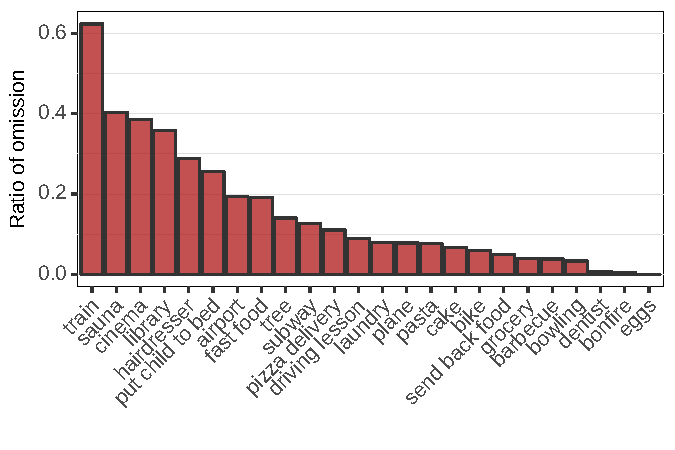
\includegraphics{figures/scr_production_omission_ratio}
 \caption{Ratio of omission across scripts.\label{fig:scripts-ellratio}}
\end{figure}


Therefore, I first investigated whether the lexicon size has an effect on the ratio of omissions in these data. In order to account for different distributions over words I also investigated a potential effect of the \textit{entropy}\is{Entropy} in this probability distributions. The entropy\is{Entropy} $H$ of a random variable quantifies the degree of uncertainty about the outcome of this variable. Following \citet[393]{shannon1948}, entropy\is{Entropy} is defined as in Equation \ref{eq:entropy}. This measure is maximal if each outcome of the variable is equally likely and it equals 0 if there is only one possible outcome.

\begin{equation}
 H\ =\ - K\ \sum_{i=1}^n  p_i \log_2  (p_i) \label{eq:entropy}
\end{equation}

Entropy\is{Entropy} might be a better predictor than the lexicon size, because entropy\is{Entropy} also reflects the shape of the probability distribution over words. If this distribution is highly skewed for a script, because there are very few very probable words, a random word in this script\is{Script knowledge} will be on average more predictable than if the distribution is relatively flat. Since I expect that information\is{Shannon information} predicts omissions, the entropy\is{Entropy} in the distribution over possible words should also predict to the ratio of omissions, possibly even better than lexicon size. Figure \ref{fig:scripts-ellratio-lexicon} illustrates the effects of lexicon size and entropy\is{Entropy} on the ratio of omissions in a script\is{Script knowledge}. The plots suggest that both a larger lexicon and a higher entropy\is{Entropy} result in a lower ratio of fragments. As entropy\is{Entropy} increases with lexicon size, both are highly correlated \correlation{0.8}{6.3}{\highsig}. Linear regressions predicting fragment ratio from these factors individually show that both lexicon size \lm{1}{6.18}{0.05} and entropy\is{Entropy} \lm{1}{12.49}{0.01} have a significant effect on fragment ratio. A regression that tests both predictors at once reveals that raw vocabulary size has no significant effect beyond entropy\is{Entropy} \lmnonsig{1}{0.02}{0.8}. This suggests that the different ratios of omissions between scripts are at least in part due to properties of the data that are relevant to my research questions and not only due to independent properties of the script\is{Script knowledge}. For this reason, I did not exclude any scripts from the data set for further analysis.

\begin{figure}
\begin{minipage}{.5\textwidth}\centering
  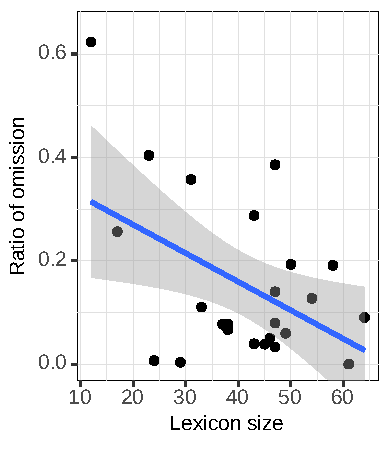
\includegraphics{figures/scr_production_omission_ratio_lexicon}
\end{minipage}%
\begin{minipage}{.5\textwidth}\centering
  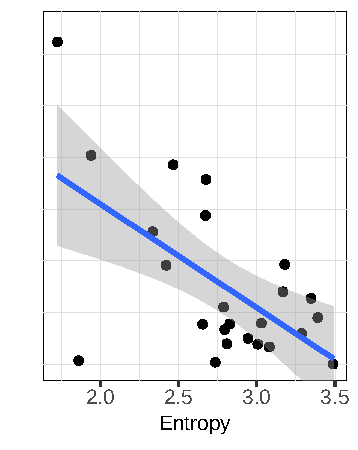
\includegraphics{figures/scr_production_omission_ratio_entropy}
\end{minipage}
 \caption{Ratio of omission as a function of lexicon size and entropy in the script.\label{fig:scripts-ellratio-lexicon}}
\end{figure}

\subsubsection{Variables}
The regression analyses described in what follows investigate effects of the three information-theoretic\is{Information theory} predictors described in the preceding section on the omission of words. \textsc{UnigramSurprisal} models the likelihood of words given extralinguistic context\is{Context, extralinguistic}, \textsc{ContextSurprisal}\is{Shannon information} additionally takes linguistic context\is{Context, linguistic} into account, and \textsc{SurprisalReduction} quantifies how much inserting a word reduces the surprisal\is{Shannon information} of the following one. Additionally, I annotated the position of the word in the utterance (numeric). As I discussed in Section \ref{sec:infotheory-uid}, in the literature there is evidence for optimization of word order\is{Word order} with respect to UID\is{Uniform Information Density}. On average, context\is{Context, linguistic} reduces the information\is{Shannon information} of words, therefore placing more informative\is{Shannon information} words toward the end of the utterance yields a more uniform ID profile\is{Information density}. In Section \ref{sec:scripts-production-results-uniformity}, I show that this prediction is borne out. Table \ref{tab:production-length} provides an overview of the distribution of utterance lengths. All preprocessed utterances had a length between one and five words. As there were only three utterances with a length of five and I analyzed utterance lengths with an ordinal model these three utterances were excluded from further analyses due to data sparseness.

\begin{table}[t]
\begin{tabular}{l *{5}{c}}
\lsptoprule
Length (words) & 1 & 2 & 3 & 4 & 5\\
\midrule
Count & 74 & 680 &1238 & 414& 3\\
\lspbottomrule
\end{tabular}
\caption{Distribution of utterances by length in the production data.\label{tab:production-length}}
\end{table}

\begin{table}[t]
\begin{tabular}{lccc}
\lsptoprule
Surprisal predictors & Pearson's $r^2$ & $t$ & $p$\\
\midrule
Unigram\is{Unigram language model}, context-dependent	& 0.65	& 70.06	& \textless 0.001\\
Unigram\is{Unigram language model}, reduction	& 0.48	& 37.99	& \textless 0.001\\
Context-dependent, reduction	& 0.62	& 54.00	& \textless 0.001\\
\lspbottomrule
\end{tabular}
\caption{Correlations between the information-theoretic predictors.\label{tab:production-correlations}}
\end{table}

\subsubsection{UID effects on omissions in fragments}
\label{sec:scripts-production-results-surprisal}

The data were analyzed with logistic mixed effects regressions predicting the outcome of the binary DV \textsc{Omission} of a word in the enriched data set from the information-theoretic\is{Information theory} measures described above. The analyses were conducted with the \texttt{lme4} package \citep{bates.etal2015} in \texttt{R} and followed the procedure described in Section \ref{sec:intro-stats}: Starting with a full model containing all fixed effects and their two-way interactions as well as a maximal random effects structure, predictors that did not significantly improve model fit (as evidenced by likelihood ratio tests) were successively removed from the model. In principle, it would be desirable to include all three predictors in a single model, but as Table \ref{tab:production-correlations} shows, they are highly correlated and regression analyses require predictors to be independent. Furthermore, effects of \textsc{SurprisalReduc\-tion} cannot be investigated for utterance-final words, which lack a following word whose surprisal\is{Shannon information} they could reduce. Therefore, I conducted three separate regression analyses. The first two analyses investigated whether \textsc{UnigramSurpri\-sal\is{Shannon information}} and \textsc{ContextSurprisal\is{Shannon information}} predict omissions. This would provide evidence for a tendency to avoid troughs in the ID profile\is{Information density}. In the third analysis I tested for an effect of \textsc{Unigram\is{Unigram language model}Surprisal\is{Shannon information}} and \textsc{Surprisal\is{Shannon information}Reduction} simultaneously, which could provide evidence for the avoidance of both peaks and troughs. This analysis was conducted on a subset of the data which excluded the utterance-final words, for which \textsc{Surprisal\is{Shannon information}Reduction} cannot be estimated.

\subsubsubsection{Avoid troughs: Effects of surprisal on omissions}
The density plots in Figures \ref{fig:production_density-unigram}\is{Unigram language model} and \ref{fig:production_density-context}  show the distribution of omissions across the range of \textsc{UnigramSurprisal}\is{Shannon information} and \textsc{ContextSurprisal}\is{Shannon information}. For both measures, the density plots suggest that on average the surprisal\is{Shannon information} of words which have originally been omitted is lower than that of realized words. The effect seems to be more pronounced for \textsc{UnigramSurprisal}\is{Shannon information}. 

\begin{figure}[p]
  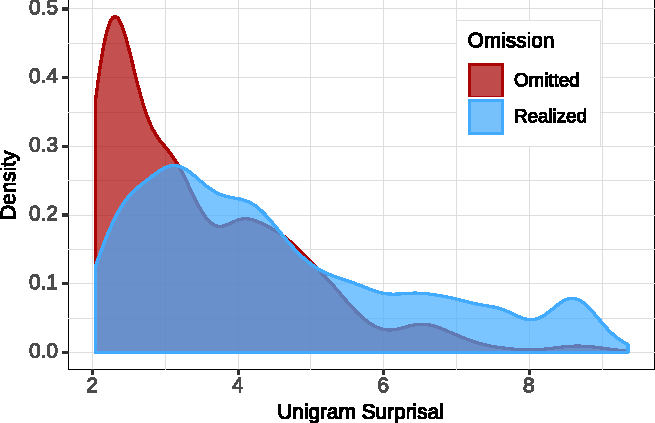
\includegraphics{figures/scr_production_density_unigram}
   \caption{The density plot shows how the omitted and realized words are distributed across the unigram surprisal scale.\label{fig:production_density-unigram}}
\end{figure}

\begin{figure}[p]
  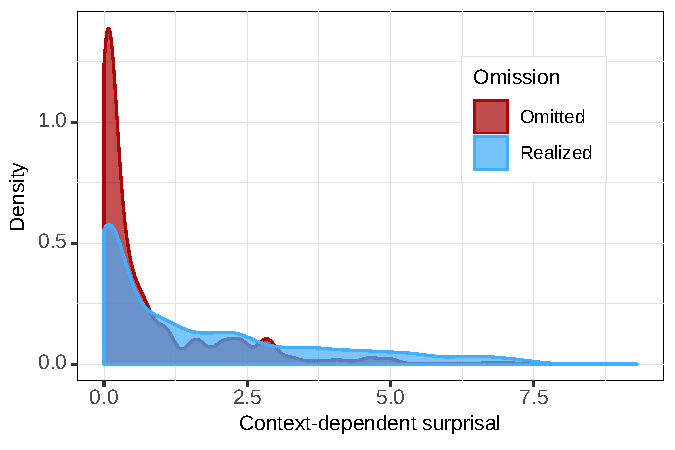
\includegraphics{figures/scr_production_density_context}
     \caption{The density plot shows how the omitted and realized words are distributed across the context-dependent surprisal scale.\label{fig:production_density-context}}
\end{figure}

The full model for unigram surprisal\is{Shannon information} contained only a main effect of \textsc{UnigramSurprisal} as well as by-subject and by-item (script) random intercepts and slopes for \textsc{UnigramSurprisal}. The by-subject effects account for individual preferences with respect to omission and the by-item effects for potential differences between scripts\is{Script knowledge}. The \textsc{UnigramSurprisal} main effect was significant \glmer{7.39}{0.01}: The lower the unigram surprisal\is{Shannon information} of a word is, the more likely it is to be omitted (see Table \ref{tab:production-unigram-estimates}). The full model for context-dependent surprisal\is{Shannon information} was identical to the one for unigram surprisal\is{Shannon information} except for the missing by-subject random slope for \textsc{ContextSurprisal}, because the model did not converge otherwise. The effect of \textsc{ContextSurprisal} was significant \glmer{4.86}{0.05} in the final model (see Table \ref{tab:production-context-estimates}).

\begin{table}
\begin{tabular}{l c c c c c}
\lsptoprule
Predictor & Estimate & SE & $\chi^2$ &  $p$ &  \\   
\midrule
\textsc{UnigramSurprisal} & -0.337 & 0.117 & 7.39 & \textless 0.01 & **\\
\lspbottomrule
\end{tabular}
\caption{Fixed effects in the final GLMM investigating the effect of \textsc{UnigramSurprisal} on \textsc{Omission}.\label{tab:production-unigram-estimates}}
\end{table}

\begin{table}
\begin{tabular}{l c c c c c}
\lsptoprule
Predictor & Estimate & SE & $\chi^2$ &  $p$ &  \\   
\midrule
\textsc{ContextSurprisal}\is{Shannon information} & -0.28 &  0.126 &  4.86 & \textless 0.05 & *\\   
\lspbottomrule
\end{tabular}
\caption{Fixed effects in the final GLMM investigating the effect of \textsc{ContextSurprisal} on \textsc{Omission}.\label{tab:production-context-estimates}}
\end{table}

Taken together, both unigram\is{Unigram language model} and context dependent surprisal\is{Shannon information} predict omissions: Words that are more predictable are more likely to be omitted. This is in line with the prediction of UID\is{Uniform Information Density} that omitting predictable words in order to avoid troughs in the density profile. A somewhat unexpected finding is that \textsc{UnigramSurprisal} seems to be a better predictor of omission than \textsc{ContextSurprisal}. In principle the opposite would be expected, because \textsc{ContextSurprisal} takes more sources of predictability\is{Context, linguistic} into account and should therefore be a more precise measure of predictability. In part, the stronger effect of \textsc{UnigramSurprisal} is probably an artifact of the data set. As the density plot in Figure \ref{fig:production_density-context} shows, the overall distribution of \textsc{ContextSurprisal} is more heavily skewed due to many words having a \textsc{ContextSurprisal} of 0. This results from the relatively small number of complete structures in my data: Sometimes one or two words suffice to completely disambiguate between the structures, so that all following words are fully redundant. An actual speaker however might have a larger set of possible utterances in mind, so that they are not as completely redundant as my model suggests. Therefore, I expect that \textsc{ContextSurprisal} would be a better predictor of \textsc{Omission} if the same procedure is applied to a larger and more diverse data set.

\subsubsubsection{Avoid peaks: Effect of surprisal reduction on omission}

In order to investigate the prediction of UID\is{Uniform Information Density} that redundancy is inserted before unpredictable words in order to smooth peaks, I conducted a third analysis that additionally considers an effect of \textsc{Surprisal\is{Shannon information}Reduction}. This analysis was conducted on a subset of the data that excluded all utterance-final words, for which \textsc{Surprisal\is{Shannon information}Reduction} cannot be estimated, and all words preceding an ellipsis. The latter were excluded because it would be unreasonable to assume that the preceding word reduced the surprisal\is{Shannon information} of an expression that had been omitted in the actual data. The subset used for this analysis contained a total of 3784 words, that is 55.52\% of the total data. The full model contained main effects of \textsc{Surprisal\is{Shannon information}Reduction} and \textsc{Unigram\is{Unigram language model}Surprisal\is{Shannon information}}, the interaction between both IVs and random intercepts for subjects and items. I chose \textsc{Unigram\is{Unigram language model}Surprisal\is{Shannon information}} rather than \textsc{ContextSurprisal\is{Shannon information}} for two reasons: First, it turned out to be a better predictor of omission than \textsc{ContextSurprisal\is{Shannon information}}, and second, as Table \ref{tab:production-correlations} shows, its correlation with \textsc{Surprisal\is{Shannon information}Reduction} is weaker than for \textsc{ContextSurprisal\is{Shannon information}} ($Pearson's\;r^2 = 0.48$ vs. $Pearson's\;r^2 = 0.62$). Table \ref{tab:production-peaks-troughs-estimates} summarizes the final model. The significant main effect of \textsc{UnigramSurprisal} \glmer{10.39}{0.01} replicates the finding of the previous analyses that predictable words are more likely to be omitted. The significant main effect of \textsc{SurprisalReduction} \glmer{27.03}{\highsig} shows that words that reduce the surprisal\is{Shannon information} of the following word more strongly are more likely to be inserted. The interaction between both predictors is not significant \glmernonsig{0.01}{0.9}. Taken together, this shows that optional omissions in fragments are driven by the tendency to avoid both troughs and peaks in the ID profile\is{Information density}, just like UID\is{Uniform Information Density} predicts.

\begin{table}
\begin{tabular}{l l l l l l}
\lsptoprule
Predictor & Estimate & \multicolumn{1}{c}{SE} & \multicolumn{1}{c}{$\chi^2$} &  \multicolumn{1}{c}{$p$} &  \\   
\midrule
\textsc{UnigramSurprisal}   &	-0.151 & 0.046 & 10.39 & \textless 0.01 & **\\
\textsc{Surprisal\is{Shannon information}Reduction} &	-0.349 & 0.07  & 27.03 & \textless \highsig & *** \\
\lspbottomrule
\end{tabular}
\caption{Fixed effects in the final GLMM investigating effects of both \textsc{UnigramSurprisal} and \textsc{SurprisalReduction}.\label{tab:production-peaks-troughs-estimates}}
\end{table}

\subsubsection{UID effects on word order}
\label{sec:scripts-production-results-uniformity}
\is{Word order|(}The production data\is{Production task} also might provide some insights into UID\is{Uniform Information Density} effects on word order\is{Word order}. UID\is{Uniform Information Density} predicts that expressions that are relatively unpredictable in the absence of linguistic context\is{Context, linguistic} tend toward being placed at the end of the utterance, because previous linguistic material reduces their surprisal\is{Shannon information}. There are two ways of testing this prediction empirically at my data set. First, following the line of reasoning taken by \citet{genzel.charniak2002}, if context reduces the surprisal\is{Shannon information} of expressions, words that are more informative\is{Shannon information} in the absence of context should be placed at the end of the utterance because this reduces their information\is{Shannon information} as compared to an initial position. Placing uninformative\is{Shannon information} words at the end of the utterance would reduce their surprisal\is{Shannon information} further and hence increase the risk of a trough in the ID profile\is{Information density}. Therefore, if UID\is{Uniform Information Density} is correct, words with a higher unigram\is{Unigram language model} surprisal\is{Shannon information} that are hence informative\is{Shannon information} in the absence of linguistic context\is{Context, linguistic}, should tend toward appearing at the end of the utterance. Second, the effect of information\is{Shannon information} reduction by preceding linguistic context\is{Context, linguistic} should be reflected in my context-dependent surprisal\is{Shannon information} measure. Therefore, words with a lower context-dependent surprisal\is{Shannon information} are predicted to appear later in the utterance.

These hypotheses were investigated with CLMMs predicting the outcome of an ordinal DV \textsc{Position} with four ordered levels from \textsc{UnigramSur\-prisal} and \textsc{ContextSurprisal}\is{Shannon information}. The analysis was conducted on the complete data set without distinguishing between originally omitted and realized words, because, if fragments are derived from regular sentences, as my experiments in the first part of this book suggest, word order\is{Word order} and omission are in principle independent from each other. Following the procedure applied in previous experiments, I started with a full model that contained main effects for both IVs, their interaction and a full random effects structure. Table \ref{tab:production-position-estimates} summarizes the final model. The position of a word in the utterance is significantly determined by both IVs. Words with a higher \textsc{UnigramSurprisal} tend to appear later \clmmLR{35.47}{\highsig}, whereas words with a higher \textsc{ContextSurprisal}\is{Shannon information} tend to appear earlier \clmmLR{41.78}{\highsig}. Both observations are in line with UID\is{Uniform Information Density}.\is{Word order|)}

\begin{table}
\begin{tabular}{l l l l l l}
\lsptoprule
Predictor & Estimate & \multicolumn{1}{c}{SE} & \multicolumn{1}{c}{$\chi^2$} &  \multicolumn{1}{c}{$p$} &  \\   
\midrule
\textsc{UnigramSurprisal} & \phantom{-}0.475  &  0.057 &  35.47 & \textless \highsig & ***\\
\textsc{ContextSurprisal}\is{Shannon information}  &  -0.585  &  0.054 & 41.78 & \textless \highsig & *** \\
\lspbottomrule
\end{tabular}
\caption{Fixed effects in the final GLMM predicting \textsc{Position} from the surprisal estimates.\label{tab:production-position-estimates}}
\end{table}

\subsubsection{Event likelihood vs. message likelihood}
\label{sec:scripts-production-results-check}
Finally, the production data\is{Production task} can also be used to test the assumption underlying the rating study\is{Acceptability rating task} that utterances referring to predictable events are more likely than those referring to unpredictable ones. If this was not the case, the results of the rating study\is{Acceptability rating task} could not be interpreted as evidence for information-theoretic\is{Information theory} well-formedness perceptions.

I addressed this question by counting how often utterances referring to the messages used in either of the predictability conditions in the rating study\is{Acceptability rating task} were produced in the production study\is{Production task}. There was a large degree of variation between scripts\is{Script knowledge}. For instance, the predictable message was produced in 96.56\% of the trials in the train script, but there were three scripts where it was never produced. Averaging over the production ratios for all scripts shows that the message tested in the predictable condition was still more often produced than that in the unpredictable condition (19.1\% vs. 0.4\% of responses). Note that the estimate for the predictable condition is rather conservative: In three scripts where the speaker buys or orders something, only those messages that refers to the item (s)he orders in the sentential condition in the rating study\is{Acceptability rating task} were counted. Taken together, this clearly confirms the reasoning underlying the rating study\is{Acceptability rating task} that predictable messages are more likely to be talked about.

\subsection{Discussion}

Experiment \ref{exp:scripts-production} provides evidence for the hypothesis that omissions in fragments are driven by a tendency to avoid peaks and troughs in the ID profile\is{Information density}. The main effects of \textsc{UnigramSurprisal} and \textsc{ContextSurprisal}\is{Shannon information} in the statistical analyses show that words that are predictable given extralinguistic\is{Context, extralinguistic} and linguistic context\is{Context, linguistic} are significantly more likely to be omitted. This reflects the tendency to avoid troughs in the ID profile\is{Information density}, which are caused by uninformative\is{Shannon information} words. The main effect of \textsc{SurprisalReduction} indicates that words that reduce the surprisal\is{Shannon information} of the next one are more likely to be realized. This evidences a strategy of reducing peaks in the ID profile\is{Information density} by inserting additional redundancy into the utterance.

Taken together, these findings indicate that UID\is{Uniform Information Density} constrains omissions in fragments. The acceptability rating\is{Acceptability rating task} data from experiment \ref{exp:scripts-rating} are also compatible with a source coding\is{Source coding} account or a general tendency to omit given or redundant material, but none of these accounts predicts the effects of the \textit{following} word's surprisal\is{Shannon information} that experiment \ref{exp:scripts-production} reveals. UID\is{Uniform Information Density} provides a natural explanation for this observation and also accounts for the finding that predictable words themselves are more often omitted.

The observation that predictable words are more likely to be omitted also implies that the choice between a fragment and a full sentence is constrained by UID\is{Uniform Information Density}. Since the experiments show that extralinguistic context\is{Context, extralinguistic} determines the predictability of individual words, the likelihood of a trough that is smoothed by the omission of predictable words is higher in predictive contexts. If the omitted word is required in a full sentence, its omission results in a fragment. This extends previous evidence for UID\is{Uniform Information Density}, where such effects were reported only for highly specific omissions of single closed-class function words to the much more diverse and semantically relevant omissions of content words in fragments. 

Experiment \ref{exp:scripts-production} investigated only omissions of words that cannot be omitted in complete sentence, like verbs and their arguments, whose omission can result in fragments. Aspects of meaning that are conveyed by e.g. temporal or locative adjuncts\is{Adjunct}, which can be implicit in full sentences, might be subject to UID\is{Uniform Information Density} too, however. Just like experiment \ref{exp:scripts-production} showed for words that can be omitted in fragments, adjuncts\is{Adjunct} might also tend to be explicit when they convey less predictable information\is{Shannon information}. Investigating omissions in adjuncts\is{Adjunct} is more complicated, because they are probably more difficult to reconstruct when they are omitted, because a potentially infinite number of adjuncts\is{Adjunct} can be inserted into an utterance. Therefore it is unclear which ones should be reconstructed and which ones should not. In the case of arguments, this reconstruction was more straightforward, because the absence of a syntactically required expression indicates that it must be reconstructed. However, in principle there is no reason to assume that the omission of adjuncts\is{Adjunct} would not be driven by UID\is{Uniform Information Density} as well.

Experiment \ref{exp:scripts-production} also provides evidence for UID\is{Uniform Information Density} effects on word order\is{Word order}. If only unigram\is{Unigram language model} surprisal\is{Shannon information}, which is independent from linguistic context\is{Context, linguistic}, is considered, unpredictable words tend toward appearing late in the utterance, just like \citet{genzel.charniak2002} showed for sentences within a text. This is expected under the assumption that the more linguistic context\is{Context, linguistic} a word has, the more predictable it becomes \citep{genzel.charniak2002, levy2008}. This assumption is in turn confirmed by the inverse effect of my context-dependent surprisal\is{Shannon information} measure which shows that the words at the end of the utterance have a lower context-dependent surprisal\is{Shannon information}. Taken together, the utterances in my data set are constrained by UID\is{Uniform Information Density} in two ways: First, UID\is{Uniform Information Density} constrains the omission of individual words, and second, otherwise unpredictable words are placed toward the end of the utterance, because its surprisal\is{Shannon information} is reduced by preceding material.

\section{The usage of fragments: Discussion}
\label{sec:scripts-discussion}

\subsection{Evidence for UID effects on omissions in fragments}
In this chapter I presented two experiments that investigated the predictions of UID\is{Uniform Information Density} the usage of fragments: (i) that predictable messages are preferably reduced, (ii) that predictable words are more likely to be omitted, and (iii) that words that reduce the surprisal\is{Shannon information} of the next word are more likely to be realized. UID\is{Uniform Information Density} shares the first prediction with source coding\is{Source coding}, but the other two are specific to UID\is{Uniform Information Density}.

Experiment \ref{exp:scripts-rating} supports the first of these predictions by showing that the reduction of predictable utterances is perceived as more well-formed than that of unpredictable ones. Somewhat surprisingly, sentences were on average preferred over fragments in both predictability conditions. This might be due to politeness considerations and the fact that some of the tested fragments are relatively improbable, as evidenced by the production data\is{Production task} collected in experiment \ref{exp:scripts-production}. Nevertheless, the experiment provides first evidence for the hypothesis that the preference for using fragments depends on the predictability of utterances. The design did not allow for the investigation of UID\is{Uniform Information Density} effects on the omission of individual words, therefore the rating study\is{Acceptability rating task} does not ultimately show whether the densification of utterances that encode likely messages is caused by the tendency to avoid peaks and troughs in the ID profile\is{Information density}, as UID\is{Uniform Information Density} predicts.

Experiment \ref{exp:scripts-production} provides evidence for the more fine-grained predictions of UID\is{Uniform Information Density} that speakers avoid peaks and troughs: Words that are themselves predictable are more likely to be omitted and words that reduce the surprisal\is{Shannon information} of following words are more likely to be inserted. The data set based on which these results were obtained was preprocessed to account for grammatical constraints on fragments. Since an optimization with respect to UID\is{Uniform Information Density} has been argued to occur only within the bounds defined by grammar \citep[25]{jaeger2010}, preprocessing ensured that each of the primitive expressions in the data set was equivalent to a constituent whose omission does not structurally depend on surrounding material. For instance, as experiment \ref{exp:pstranding-german} showed that prepositions cannot be freely omitted\is{Preposition omission} in German\il{German}, I merged the noun phrase\is{Noun phrase} and the preposition within a PP\is{Preposition phrase} to a single primitive unit. Experiment \ref{exp:scripts-production} provides clear evidence for UID\is{Uniform Information Density} effects on individual omissions in fragments. This conclusion implies that the choice between producing a fragment and producing a full sentence in a specific situation is also constrained by UID\is{Uniform Information Density}: In unpredictive contexts\is{Context, extralinguistic}, the probability of troughs in the ID profile\is{Information density}, which trigger omissions, is lower than in predictive ones. If no words that are obligatory in full sentences are omitted for this reason, the speaker will prefer to utter a full sentence rather than any of the grammatically possible fragments. This extends previous evidence for UID\is{Uniform Information Density}, where such effects were reported only for highly specific omissions of closed-class function words to the much more diverse omissions of content words in fragments.

Experiment \ref{exp:scripts-production} furthermore provides evidence for UID\is{Uniform Information Density} effects on word order\is{Word order}: Words with a higher unigram\is{Unigram language model} surprisal\is{Shannon information}, which are less predictable in the absence of context, tend to appear late in the utterance. The UID\is{Uniform Information Density} explanation for this observation is that linguistic context\is{Context, linguistic} reduces the surprisal\is{Shannon information} of words that are otherwise unpredictable. Therefore, as \citet{fenk-oczlon1983} argues, placing predictable words before uninformative\is{Shannon information} ones yields a more uniform ID profile\is{Information density}. The assumption that linguistic context\is{Context, linguistic} increases the predictability of words on average is supported by the inverse effect of context-depen\-dent surprisal\is{Shannon information}, where predictable words tend to appear \textit{late} in the utterance. Experiment \ref{exp:scripts-production} thus also provides empirical evidence for a (reasonable) assumption that has only been stipulated in previous work \citep{fenk-oczlon1983, fenk-oczlon1989, genzel.charniak2002}.

\subsection{UID vs. availability-based production}

Following \citet{hale2001}, I assume that the relationship between the likelihood of a word and its omission is determined by processing effort\is{Processing effort}. Speakers perform audience design\is{Audience design} by adapting their message to  the expected cognitive resources of the hearer, and omissions occur whenever they are beneficial to that goal. However, as I sketched in Section \ref{sec:infotheory-uid-competing-abp}, predictability effects have also been explained with the effort required to retrieve a word from memory alone. \is{Availability-based production|(}Availability-based production\is{Availability-based production} predicts that omissions occur more often if the word following the omitted one is predictable and hence easy to retrieve, as \citet{ferreira.dell2000} show for complementizer omission\is{Complementizer omission} in English\il{English}. The same effect is predicted by UID\is{Uniform Information Density}, but for a different reason: Realizing words that precede unpredictable words can reduce the surprisal\is{Shannon information} of the latter and hence smooth peaks in the ID profile\is{Information density}. The observation that words are more likely to be inserted before unpredictable words can therefore be also interpreted as an effect of availability-based production. As \citet{jaeger.buz2017} note, availability-based production and UID\is{Uniform Information Density} are not mutually exclusive and there might be independent effects of both theories, but in case both theories predict the same effect it cannot be attributed unambiguously to either of the theories.

Effects of availability-based production\is{Availability-based production} however are particularly expected in oral communication, because according to \citet{ferreira.dell2000} the motivation for inserting optional words is to avoid disfluencies which would result from the time required to retrieve unpredictable lemmas from memory. This is the case in studies on spoken corpora\is{Corpus} \citep{levy.jaeger2007, frank.jaeger2008, jaeger2010} or spoken production experiments \citep{kurumada.jaeger2015, norcliffe.jaeger2016}, but it does not concern my production study\is{Production task} (experiment \ref{exp:scripts-production}) in the same way: Even though I asked subjects to provide utterances that seem natural in a situation of oral communication, they provided written responses, so there is no risk of disfluencies. Therefore, even though some of the evidence for UID\is{Uniform Information Density} might be explained by production alone, this explanation is less convincing in case of the effects that I found in my production study\is{Production task}.

Furthermore, availability-based production\is{Availability-based production} can only explain why the omission of a target word can be predicted from the surprisal\is{Shannon information} of the following word(s), but not why it depends on the target word's own surprisal\is{Shannon information}. Most of the previous studies on UID\is{Uniform Information Density} and my production study\is{Production task} found that the predictability of the target word itself predicts its omission as well. Taken together, the predictions of UID\is{Uniform Information Density} and availability-based production\is{Availability-based production} partially overlap, and specifically in studies on spoken language some of the effects of UID\is{Uniform Information Density} can be explained by availability-based production\is{Availability-based production} as well. However, availability-based production\is{Availability-based production} cannot account for all of the data, and specifically in my experiments the written modality makes it implausible that omissions depend on the likelihood of disfluencies. This does not speak against the idea of availability-based production\is{Availability-based production}, but it provides distinctive evidence for UID\is{Uniform Information Density}.\is{Availability-based production|)}

\subsection{Information theory or information structure?}
\is{Information theory|(}\is{Information structure|(}The information-theoretic\is{Information theory} account that I pursue often coincides with a perspective based on information structure\is{Information structure}, which requires omitted expressions to be e-given\is{E-givenness} \citep{merchant2004}, not part of the focus \citep{reich2007} or backgrounded \citep{ott.struckmeier2016}. Words that are predictable are probably often given in a possibly implicit QuD\is{Question under Discussion}. For instance, in the taxi example that I used to illustrate my approach above, it is reasonable to assume that a QuD\is{Question under Discussion} like \textit{Where should I take you?} licenses ellipsis of everything but the focused word corresponding to the \textit{wh}-phrase in the answer. From an information-structural\is{Information structure} perspective, given material \textit{can} be omitted because it is given, and from an UID\is{Uniform Information Density} perspective it \textit{should} be omitted, since it would probably yield a trough in the ID profile\is{Information density}. A potential testing ground to distinguish between information structure and information theory are expressions that are given, but not predictable, or vice versa. Givenness and predictability might coincide most of the time though, so that distinguishing between these concepts requires a set of constructed materials for which the predictability of a given expression can be manipulated.

The main difference between an information-theoretic\is{Information theory} and an information-structural\is{Information structure} approach to the usage of fragments, however, is that only information theory\is{Information theory} can  explain why an expression actually is (not) omitted. Information-structural concepts like givenness might license ellipsis, but it is clearly not necessary to omit each given expression. For instance, it is appropriate to answer a question with a full sentence even though most of the words contained in the answer are given. In contrast, UID\is{Uniform Information Density} provides an account of why particular words are preferably omitted and of why they might be realized. Information structure does also not explain why the surprisal\is{Shannon information} of the word that follows a target word has an effect of the target word's omission. This does not neglect the role of information structure on omissions though, and it is very likely that information-theoretic\is{Information theory} concepts like givenness are reflected in and should be taken into account by more sophisticated measures of surprisal\is{Shannon information}.\is{Information theory|)}\is{Information structure|)}

\subsection{Script knowledge as models of extralinguistic context}
Since fragments often appear discourse-initial\is{Fragment, discourse-initial}ly, the predictability of words in context is determined to a large extent by extralinguistic context\is{Context, extralinguistic}, which cannot be captured by standard language modeling techniques applied to speech corpora\is{Corpus}. Therefore, the context stories used in experiments \ref{exp:scripts-rating} and \ref{exp:scripts-production} were based on probabilistic event chain\is{Event chain}s extracted from the DeScript corpus\is{Corpus} of script knowledge\is{Script knowledge} \citep{wanzare.etal2016}, which contains crowdsourced descriptions of the stereotypical time-course of script\is{Script knowledge} events.

The rating study\is{Acceptability rating task} shows that utterances referring to predictable events were more acceptable, and that this holds in particular for fragments. I interpreted this as evidence for optimization of the signal with respect to information-theoretic\is{Information theory} principles because I assumed that predictable events would be more likely to be talked about. The production data\is{Production task} collected in experiment \ref{exp:scripts-production} confirms that this corpus\is{Corpus}-based predictability manipulation in experiment \ref{exp:scripts-rating} is overall in line with subjects' expectations about upcoming utterances. The utterances in the predictable condition in the rating study\is{Acceptability rating task} had an average likelihood  of 19.1\%, whereas those in the unpredictable condition were produced only in 0.4\% of the trials in the production task. Note that this is a conservative estimate since for instance in the pizza ordering scenarios, utterances were classified as encoding a different message depending on what the customer orders.

This manipulation did not work equally well for all scripts\is{Script knowledge}. In three scenarios, the presumably predictable message was never produced and some of the unpredictable fragments that were never produced received relatively high ratings. Consequently, there was no significant correlation between message frequency and the acceptability\is{Acceptability rating task} of fragment conditions. As I discuss in Section \ref{sec:fragments-game} below, the optimality of fragments might not be driven by message frequency alone, but also by the utility of the fragment to unambiguously communicate a message.

On average though, utterances referring to predictable events turned out to be more likely in the production study\is{Production task}. This supports the procedure that I used for constructing materials for experiments \ref{exp:scripts-rating} and \ref{exp:scripts-production} and shows that, even though scripts\is{Script knowledge} do not cover \textit{all} aspects of extralinguistic context\is{Context, extralinguistic}, script\is{Script knowledge} corpora\is{Corpus} provide precise estimates of the likelihood of utterances in context and therefore constitute a empirically sound approximation to extralinguistic context\is{Context, extralinguistic}.

\subsection{Surprisal estimation in elliptical data}

The conclusions drawn from experiment \ref{exp:scripts-production} rely on a novel method to estimate surprisal\is{Shannon information} that is robust to a circularity issue caused by ellipses in the training data: If predictable words are omitted more often, their predictability is not proportional to their corpus\is{Corpus} frequency because they are often omitted. This would distort predictability estimates calculated with regular language models. My approach avoids this problem, because it relies on nonelliptical data for estimating surprisal\is{Shannon information}. The method is similar to the approach proposed by \citet{hale2001}, who derives surprisal\is{Shannon information} from the probability mass of the parses\is{Parser, parallel} that are disconfirmed by an input. Like \citeauthor{hale2001}'s method, it is fully incremental, i.e. the information that a word provides to the parser\is{Parser, human} is used as soon as this word is encountered. The method is also psychologically realistic, because only those words that are available to the hearer are included in the context\is{Context, linguistic} used for surprisal\is{Shannon information} estimation. Words that are omitted in context of the target word have no effect on its surprisal\is{Shannon information}.

The significant effect of context-dependent surprisal\is{Shannon information} in the analysis shows that is a suitable approximation to the information\is{Shannon information} of words in context. However, the effect of unigram\is{Unigram language model} surprisal\is{Shannon information} on omission was stronger than that of context-dependent surprisal\is{Shannon information} even though I expected the opposite because context-depen\-dent surprisal\is{Shannon information} takes more sources of predictability into account. This might be due to the relatively small size of my data set, for which sometimes a sequence of two words completely disambiguates between parses. All following words necessarily receive a surprisal\is{Shannon information} of 0. I expect stronger effects of context-dependent surprisal\is{Shannon information} in larger and more diverse data sets. Linguistic context\is{Context, linguistic} might also be more important when syntactic information, like inflectional marking on verbs, is more prominent. Other measures of context-dependent surprisal\is{Shannon information}, such as word likelihoods derived from a PCFG\is{Context-free grammar} \citep{hale2001} are sensitive to hierarchical syntactic information, such as subcategorization preferences, for instance that of a preposition for a DP\is{Determiner phrase} or specific verbs for a complementizer. Such function words had been removed from my data set during preprocessing.

The data set collected in experiment \ref{exp:scripts-production} was elicited with a set of carefully built context stories and required a considerable amount of manual preprocessing, which consisted in the unification of synonyms, annotation of case morphology and prepositions, removal of adverbials\is{Adverbial} and the reconstruction of ellipses. Since the analysis confirmed the validity of this approach, it might be interesting to explore to which extent it can be automatized, e.g. by automatic unification of synonyms, morphosyntactic annotation and reconstruction of ellipsis. In such research, the manually preprocessed data can be used as a gold standard for the evaluation of automatized preprocessing procedures.

\section[Outline of a game-theoretic model of fragment usage]{Outline of a game-theoretic model of fragment usage}

\label{sec:fragments-game}

This section outlines a possible game-theoretic\is{Game theory} account of fragments, which can potentially explain some aspects of the choice between a fragment and a full sentence that UID cannot. Empirically testing such an account and comparing its predictions to UID\is{Uniform Information Density} is intricate and must therefore be left to future research.

\subsection{Limits of UID effects on the form of utterances}

The regression approach that I took in the analysis of experiment \ref{exp:scripts-production} predicts the omission of individual words within a complete sentence from information-theoretic\is{Information theory} variables, such as the surprisal\is{Shannon information} of the target word or how much this word's insertion reduced that of the word following it. However, as I noted in section \ref{sec:infotheory-uid}, UID\is{Uniform Information Density} faces an empirical problem when a single fragment can be derived from a predictable and an unpredictable sentence. For the purpose of illustration, consider the situation where the fragment in \Next[a] is used to communicate the full sentences in \Next[b] or \Next[c] in the taxi scenario discussed above (the probabilities associated with each complete structure are hypothetical).

\ex. \a. To the university.
    \b. Take me to the university. \hfill $p = 0.2$
    \c. Tell me the way to the university.\hfill $p = 0.05$
    \d. [other messages, cumulated] \hfill $p = 0.75$

This issue concerns the usage of the fragment in order to communicate \Last[c]. The ID profile Figure \ref{fig:fragments-uid-unpredictable} suggested that omitting \textit{tell me the way} would result in a peak in the ID profile\is{Information density} that can be avoided by inserting these words, but I already noted there that this is a simplification. Since a hearer who perceives the fragment in \Last[a] does not know whether it has been derived from \Last[b] or \Last[c], processing the fragment must be equally effortful\is{Processing effort} in both cases. Therefore, the fragment will either exceed channel capacity in both cases or in neither of them. %

The problem with encoding the unpredictable \Last[c] with the fragment in \Last[a] therefore is not a peak in the ID profile\is{Information density}, but that a hearer who encounters the fragment in the scenario in \Last has to guess whether the speaker intended to convey \Last[b], \Last[c] or another message. Intuitively, he will go for the more likely \Last[b],% 
% 
\footnote{Only those messages that a fragment can potentially encode will be considered, i.e. those from which the fragment can be derived by ellipsis. For instance, \Last[a] can be derived from \Last[b] and \Last[c], whereas \textit{Take me to the airport} is not a possible source for \Last[a].}\afterfn%
%
because the speaker is more likely to intend to communicate this message than \Last[c]%
%
\footnote{Note that this is also in line with the source coding\is{Source coding}-based prediction that more frequent messages are assigned shorter codes.}\afterfn%
%
and the hearer is consequently more likely to interpret the utterance as intended. UID\is{Uniform Information Density} is by definition unable to take this difference between meanings into account because it models only the encoding procedure, i.e. the choice of the most well-formed utterance to communicate a specific message given the properties of the communication system. Decodingm, the choice of a message given a received signal, is simply not covered by UID\is{Uniform Information Density}.

Before discussing a potential solution to this issue, note that this is a conceptual problem rather than an empirical one. The speaker does neither know with certainty the capacity\is{Channel capacity} of the channel nor the hearer's probability distribution over possible complete structures that determines surprisal\is{Shannon information}. Therefore, all she can do is omit words that are \textit{more likely} to yield a trough and to insert those that are \textit{more likely} to smooth a peak in the ID profile\is{Information density}. From this perspective, she will omit the predictable \textit{take me} in \Last[b] and realize the less predictable \textit{tell me the way} in \Last[c]. The unpredictable \textit{to the university} will be preferably realized in both situations.

\subsection{Game-theoretic pragmatics}
\is{Game theory|(}A framework that might overcome this problem is game-theoretic\is{Game theory} pragmatics. Game-theoretic approaches provide a model of context\is{Context, extralinguistic} which takes into account the knowledge and preferences of rational agents. The model allows for determining which action is the most useful one to pursue for each of the agents. Such models have been recently gaining popularity in pragmatics and been applied to phenomena like implicature \citep{vanrooy2004, benz.vanrooij2007, franke2009, jager2012, goodman.stuhlmuller2013, gotzner.benz2018} and reference \citep{frank.goodman2012, rohde.etal2012, sikos.etal2019}. \is{Iterated Best Response model|(}In what follows I base my expositions on the approach taken by \citet{franke2009}, who develops a game-theoretic\is{Game theory} account of pragmatic reasoning that models implicatures, the \textit{Iterated Best Response} (IBR\is{Iterated Best Response model}) model. He interprets communicative situations as signaling games, which are played by a speaker and a hearer and require a speaker to pick an utterance in order to get a message across.%
%
\footnote{The terminology used in the game-theoretic\is{Game theory} literature differs from the one that I use, which I maintain in order to keep the mapping between terms and concepts throughout this book. In the game-theoretic\is{Game theory} literature, the utterance is called the \textit{message} and what is being communicated (I use the term \textit{message} for this) is labeled the \textit{state}.}\afterfn%
%
Even though Franke investigates a different phenomenon, the problem of mapping utterances and interpretations remains the same, so in principle it can be straightforwardly applied to the interpretation of fragments.

The main ingredients of a signaling game are a set of possible messages, i.e. meanings that the speaker could intend to communicate, a set of possible interpretation actions, that is, meanings that the hearer could assign the utterance and a set of utterances that can be used for this purpose. Only the speaker knows with certainty which message she wants to convey, and she has to choose the utterance that she believes to be the best one to get a message across. The hearer has to figure out which message the speaker intended to communicate. In this setting, both the speaker and the hearer initiate a chain of recursive reasoning about each other which result in the choice of an utterance and the assignment of a meaning (a message) to this utterance. Which utterance is most optimal from the speaker perspective and which meaning the hearer assigns to it depends on a series of parameters: First, the messages often differ in their \textit{prior probability} before any utterance is produced. In the case of the taxi example, it might be more likely that people would ask for a ride than that they would ask for directions. Second, the production of some utterances can be more effortful and hence costly. Third, a single utterance can sometimes encode more than one message, and a single message can be referred to by more than one utterance. Finally, game-theoretic\is{Game theory} models may include varying payoffs that each participant receives depending on her own and the other player's choices. In linguistic applications, where the speaker wants to get a message across and the hearer wants to figure it out correctly, the payoffs for both interlocutors are aligned, since both share the goal of successful communication \citep[21]{franke2009}. In what follows I present a simplified sketch of how \citet[59--61]{franke2009} applies this model to scalar implicature before I illustrate how this reasoning can be extended to fragments.

\subsection{Game-theoretic modeling of scalar implicatures}
For scalar implicatures, \citet{franke2009} focuses on the interpretation of the quantifier \textit{some} as \textit{some but not all}. Despite theoretical and empirical debates on how exactly this interpretation is generated \citep[see e.g.][]{levinson1983, levinson2000, sperber.wilson1986, vankuppevelt1996, breheny.etal2006, huang.snedeker2009, grodner.etal2010}, the general observation is that utterances like \Next[a] are often interpreted as \Next[b], even though semantically \Next[a] is implied by and hence does not rule out \Next[c].

\ex. \a. Some of students completed the assignment.
     \b. Some but not all of the students completed the assignment.
     \c. All of the students completed the assignment.

\citet[59--61]{franke2009} models this situation with a reference game, whose parameters are given in Table \ref{tab:gt-si}. In the game there are only two possible meanings, $m_{\exists\neg\forall}$ and  $m_{\forall}$, two corresponding interpretation actions $a_{\exists\neg\forall}$ and  $a_{\forall}$ and two possible utterances, $u_{some}$ and $u_{all}$. The two utterances correspond to \Last[a,c] respectively. Whereas $u_{some}$ is true in case of both messages, $u_{all}$ is false if $m_{\exists\neg\forall}$ is true. Therefore, $u_{all}$ may be selected only if that the speaker wants to communicate that all students completed the assignment. Each of the messages has a prior probability $Pr(m)$. As I noted above, under the assumption that both agents pursue the goal of successful communication, the payoffs for speaker and hearer are matched: Both receive a payoff of 1 if the interpretation action corresponds to the intended message and no payoff if it does not.
     
\begin{table}
 \begin{tabular}{l c c c c c c}
 \lsptoprule
  & Pr(m) & $a_{\exists\neg\forall}$ & $a_{\forall}$ & $u_{some}$ & $u_{all}$\\
  \midrule
 $m_{\exists\neg\forall}$ & 1 -- p & 1,1 & 0,0 & \ding{51} & -- \\
  $m_{\forall}$ & p & 0,0 & 1,1 & \ding{51} & \ding{51} \\
  \lspbottomrule
 \end{tabular}
 \caption{Tableau for the scalar implicature game, adapted from \citet[21]{franke2009}. The table provides the probability $Pr(m)$ for each message, the speaker and hearer payoffs for each combination of messages and interpretation actions and determines which utterance can be used to communicate each message.\label{tab:gt-si}}
 \end{table}
 
Based on this setting, two chains of iterative reasoning of the agents about each other's behavior are initialized. One of these chains starts with a \textit{literal} speaker and the other one with a literal hearer. Unlike higher order \textit{pragmatic} agents, literal agents take only the general setup of the model into account but do not reason about the other agent's behavior. The literal speaker selects randomly an utterance that is true. In order to communicate $m_{\exists\neg\forall}$, the only available utterance is $u_{some}$, because $u_{all}$ is false in this situation. In contrast, $m_{\forall}$ can be communicated with both utterances, because both are true for this message. This yields the following \textit{strategies}:


\begin{equation}
S_0 = \begin{Bmatrix} t_{\exists\neg\forall} \mapsto m_{some}\\
        t_{\forall} \mapsto m_{some}, m_{all}\\
       \end{Bmatrix}
\end{equation}

The literal hearer calculates the posterior probability of each message to be intended by the speaker given each of the available utterances. The listener does not reason about the speaker's behavior and considers only the prior probability of each message and the truth conditions. In the first sketch of his approach, \citet{franke2009} uses flat priors ($p = 0.5$). Table \ref{tab:gt-si-l0} summarizes the posterior probabilities for the scalar implicature game. If the hearer encounters $u_{all}$, the posterior probability of $\mu(m_{\exists\neg\forall}|u_{all})$ equals 0, because the utterance would be false in case of the message. Therefore, $\mu(m_{\forall}|u_{all}) = 1$, because this is the only message for which $u_{all}$ is true. If the hearer encounters $u_{some}$, both messages could be true, so he will go for the most likely one in order to maximize the likelihood of figuring out the intended meaning. Since both messages are equally likely in case of flat priors, assigning an interpretation to the utterance consists in random guessing.%
%
\footnote{However, if $m_{\exists\neg\forall}$ is more likely than $m_{\forall}$ (if $p > 0.5$), assuming that the more likely message was intended increases the probability of success.}\afterfn%
%
This yields the interpretation strategies in Table \ref{tab:gt-si-l0}: $u_{some}$ will be interpreted either as $m_{\exists\neg\forall}$ or $m_{\forall}$, whereas $u_{all}$ will be always interpreted as $m_{\forall}$:

\begin{equation}\label{eq:l0}
 L_0 = \begin{Bmatrix} u_{some} \mapsto m_{\exists\neg\forall},m_{\forall}   \\
        u_{all} \mapsto m_{\forall}\\
       \end{Bmatrix}
\end{equation}

\begin{table}
\begin{tabular}{c c c}
 \lsptoprule
 $\mu_0(m|u)$ & $m_{\exists\neg\forall}$ & $m_{\forall}$\\
\midrule
$u_{some}$ & ½ & ½ \\
$u_{all}$ & 0 & 1\\
\lspbottomrule
\end{tabular}
\caption{Posterior probabilities for the literal hearer $L_0$.\label{tab:gt-si-l0}}
\end{table}

The pragmatic speaker takes into account these interpretation strategies of the literal hearer. Since the hearer will unambiguously interpret $u_{all}$ as $m_{\forall}$ but might understand $u_{some}$ as either of the messages, $u_{all}$ has a higher \textit{utility} than $u_{some}$ to communicate $m_{\forall}$. In order to communicate $m_{\exists\neg\forall}$ the utility of $u_{all}$ is 0. Even though a literal hearer might interpret $u_{some}$ as $m_{\forall}$ half of the time, $u_{some}$ is the more promising option for the speaker to get the message across. This results in the following strategies:

\begin{equation}
 S_1 = \begin{Bmatrix} t_{\exists\neg\forall} \mapsto m_{some}\\
        t_{\forall} \mapsto m_{all}\\
       \end{Bmatrix}
\end{equation}

The pragmatic hearer calculates the posterior probability for each message given each utterance, but unlike $L_0$ he takes not only the priors but also the strategies of $S_0$ into account. He calculates the product between the prior probability of a message $m$ and $S_0$ uses a $m$ to encode this message, which is divided by the sum of this term for each message in this situation that $u$ could potentially encode as well \citep[27]{franke2009}:

\begin{equation}
\displaystyle \mu(m|u) = \frac{Pr(m) \times \sigma (u|m)}{\sum_{m'\in M} Pr(m') \times \sigma(u|m')} %)
\end{equation}

This measure increases the higher the prior probability of $m$ is and the more likely $u$ is to be used to encode $m$ as compared to the alternative messages $m'$. In the case of the scalar implicature this yields the posterior probabilities in Table \ref{tab:gt-si-l1}, which, applying the same reasoning as above, result in the interpretation strategies that are in line with the encoding preferences of $S_1$ \ref{eq:gt_l1}:%
%
\footnote{For a more detailed discussion of the formula see \citet[26--27]{franke2009} and for the application to scalar implicatures \citep[60]{franke2009}.}\afterfn%
%

\begin{equation}
L_1 = \begin{Bmatrix} u_{some} \mapsto m_{\exists\neg\forall} \\
        u_{all} \mapsto m_{\forall}\\
       \end{Bmatrix}\label{eq:gt_l1}
\end{equation}

This model is of course highly simplified because it avoids further alternative expressions and interpretations, such as other quantifiers (\textit{many}, \textit{most}, etc.) and the more explicit, but longer \textit{some but not all}.%
%
\footnote{Effects of a \textit{some but not all} message are discussed by \citet[77, 127]{franke2009}.}\afterfn%
%
Still though, it can model scalar implicatures both on the side of the hearer and on that of the hearer after only one recursive iteration step. The strategies of $L_1$ or $S_1$ can also be the input to higher order reasoning processes.\is{Iterated Best Response model|)}\is{Game theory|)}

\begin{table}
\begin{tabular}{c c c}
 \lsptoprule
 $\mu_0(m|u)$ & $m_{\exists\neg\forall}$ & $m_{\forall}$\\
\midrule
$u_{some}$ & ⅔ & ⅓ \\
$u_{all}$ & 0 & 1\\
\lspbottomrule
\end{tabular}
\caption{Posterior probabilities for the pragmatic hearer $L_1$.\label{tab:gt-si-l1}}
\end{table}

\subsection{Application to fragments}
The case of fragments is often more complex than the (simplified) scalar implicature example discussed above. However, the underlying situation is similar, even though the set of messages and utterances is considerably larger: There is a set of possible messages that the speaker might want to communicate to the hearer and a set of utterances that she can use for this purpose. The sets of possible messages and utterances are potentially extremely large (if not infinite, due to recursion in language), but in situations that are constrained by script knowledge\is{Script knowledge} (like in the data from experiment \ref{exp:scripts-production}), the set of actually considered alternative messages and utterances is often relatively limited.  Consider a simplified version of the pasta scenario which I used to illustrate the surprisal calculation methods in Section \ref{sec:scripts-production-surprisal}. In this version of the scenario there are only two messages with differing prior probabilities, which are given in \Next. Again, I use the representations that resulted from preprocessing the production data\is{Production task} collected with experiment \ref{exp:scripts-production}. Each message $m_i$ has is associated a (hypothetical) prior probability $Pr(m_i)$.

\ex. \a. \texttt{pour pasta pot} \hfill $Pr = 0.6$
     \b. \texttt{pour salt pot} \hfill $Pr = 0.4$

Under the assumption that each ``word'' in these utterances can be omitted independently from the surrounding words, the set of possible utterances is:

\begin{equation}
 U = \begin{Bmatrix}
       pour \mathspace pasta \mathspace pot, pour \mathspace salt \mathspace pot,\\
       pour \mathspace pasta, pour \mathspace pot, pour \mathspace salt, pasta \mathspace pot, salt \mathspace pot,\\
       pour, pasta, pot, salt
      \end{Bmatrix}
\end{equation}

Even in this highly simplified scenario with only two messages that differ only in one word, there are 11 possible utterances. The combination with the two messages in \Last yields the tableau in Table \ref{tab:gt-fragments-truth}, based on which the same reasoning steps like in the scalar implicature example can be performed. If more meanings were considered, the complexity of the tableau would increase, but the problem remains identical.

\begin{table}
\begin{tabular}{l l p{.34cm} p{.34cm} p{.21cm} p{.21cm} p{.21cm} p{.21cm} p{.21cm} p{.21cm} p{.21cm} p{.21cm} p{.21cm} p{.21cm} p{.21cm} p{.21cm}}
\lsptoprule
Message & Pr(m) & \rotatebox{90}{$a_{pour \mathspace pasta \mathspace pot}$} & \rotatebox{90}{$a_{pour \mathspace salt \mathspace pot}$} & \rotatebox{90}{\texttt{pour pasta pot}} & \rotatebox{90}{\texttt{pour salt pot}} & \rotatebox{90}{\texttt{pour pasta}} & \rotatebox{90}{\texttt{pour pot}} & \rotatebox{90}{\texttt{pour salt}} & \rotatebox{90}{\texttt{pasta pot}} & \rotatebox{90}{\texttt{salt pot}} & \rotatebox{90}{\texttt{pour}} & \rotatebox{90}{\texttt{pasta}} & \rotatebox{90}{\texttt{pot}} & \rotatebox{90}{\texttt{salt}}\\
\midrule
$m_{pour \mathspace pasta \mathspace pot}$ & 0.6 & 1,1 & 0,0 & \ding{51} & -- & \ding{51} & \ding{51} & -- & \ding{51} & -- & \ding{51} & \ding{51} & \ding{51} & --  \\
$m_{pour \mathspace salt \mathspace pot}$ & 0.4 & 0,0 & 1,1 & -- & \ding{51} & --  & \ding{51} & \ding{51} & --  & \ding{51} & \ding{51} & -- & \ding{51} & \ding{51}\\
\lspbottomrule
\end{tabular}
\caption{Tableau for the simplified pasta scenario game. \label{tab:gt-fragments-truth}}
\end{table}

Applying game-theoretic\is{Game theory} reasoning to the production and interpretation of fragments requires a conceptual and a methodological modification to the approach by \citet{franke2009}. The theoretical modification concerns the relationship between utterances and messages. In the case of \citeauthor{franke2009}'s model, there are only complete utterances, and truth conditions determine whether an utterance is suitable for communicating a message. In the case of fragments however, it is not reasonable to assume that a noun phrase\is{Noun phrase} like \textit{pasta} is \textit{true} in a situation. Instead, the relationship between utterances and messages can be modeled by the suitability of an utterance to communicate a message: An utterance is classified as suitable for communicating a message if it can be derived by an arbitrary number of omissions from the message's full form: \texttt{pour pasta} can be derived from $m_{pour \mathspace pasta \mathspace pot}$ by omitting \texttt{pot}, whereas it cannot be derived from $m_{pour \mathspace salt \mathspace pot}$. Of course, this is a further simplification, because in reality each message can be encoded by a variety of nonelliptical utterances, which differ in the choice of lexical items and word order, among other properties. However, in principle the same reasoning can be applied to this situation: The set of utterances that can encode a message is restricted to those expressions that can be generated by grammatically licensed omissions from the set of full sentences that can encode this message.

The methodological problem concerns ambiguous\is{Ambiguity} fragments. Since speakers use fragments, so it is reasonable to assume that in some situations fragments are more useful encodings than full sentences, so the model must allow for this outcome. However, the model so far predicts that fragments are sometimes as good as sentences, but never better than them: Complete sentences unambiguously identify the message intended by the hearer, so they are always preferred over potentially more vague fragments, just like the unambiguous\is{Ambiguity} $u_{all}$ has the highest utility in the scalar implicature game by \citet{franke2009}. Even though, at least in the example presented here, fragments like e.g. \texttt{salt} or \texttt{pasta} share this property, in this situation they are not preferred over the full sentence. The main advantage of fragments is that they perform the same function as sentences in less time and with a reduced production effort for the speaker. Therefore, it is reasonable to integrate a cost term into the model, which reduces the speaker utility of longer utterances by discounting a percentage of the utility for each word. This models the speaker's preference for producing shorter utterances, which will favor unambiguous\is{Ambiguity} fragments in the case of my example. In large-scale applications the cost term might even favor potentially ambiguous\is{Ambiguity} fragments, if the prior probability of the message as compared to competing messages and the reduction of production cost are large enough to outweigh the remaining ambiguity\is{Ambiguity}.

\subsection{Application to natural language data}
In principle it is possible to apply this model to the data set collected with experiment \ref{exp:scripts-production}. This data set contains an annotation layer of the message underlying each utterance, so that the prior probability of each of message in the scenario can easily be calculated. Based on the preprocessed data set it is also straightforward to determine which complete structures can used to communicate each message and hence to specify (i) the set of possible utterances and (ii) whether each of these utterances can be used to communicate a message. However, the simple example above showed that even when there are only two possible messages there are 11 possible utterances. Consequently, the about 100 utterances produced for each scenario in experiment \ref{exp:scripts-production} do not allow for a fine-grained investigation of the relationship between game-theoretic\is{Game theory} utility and omission. A larger and more homogeneous data set would be required to investigate the predictions of a game-theoretic\is{Game theory} account of fragment usage in detail.

\subsection{Implications and comparison to UID}
Even though I argued in the introduction to this section that UID\is{Uniform Information Density} and game theory\is{Game theory} make partially overlapping predictions on omissions in fragments, they differ with respect to which aspects of communication they model, the mechanism that derives their predictions, and some empirical predictions.

Game theoretic pragmatics\is{Game theory} models both the behavior of the speaker and the hearer, whereas UID\is{Uniform Information Density} focuses on the speaker and accounts only for encoding but not for decoding. The hearer is taken into account indirectly, since the speaker adapts the signal to the cognitive resources\is{Processing effort} she assumes the hearer to possess. The game-theoretic approach explicitly models the actions performed by both agents, as well as their expectations and preferences. By focusing on encoding, UID\is{Uniform Information Density} compares and ranks the usefulness of various utterances to communicate a single message, and the properties and the likelihood of alternative messages are considered only insofar as they contribute to the surprisal\is{Shannon information} of words. This ignores the possibility that an utterance is falsely interpreted as another message than the one intended by the speaker. In contrast, the game-theoretic account predicts a preference for more explicit forms if the intended interpretation is not the most likely one if a fragment was used.

UID\is{Uniform Information Density} and the game-theoretic\is{Game theory} approach also attribute production preferences to different mechanisms. Whereas UID\is{Uniform Information Density} is a psycholinguistic theory based on the efficient distribution of processing effort\is{Processing effort} (in the interpretation that I adopt) or efficient communication in the presence of noise and is relatively indifferent to meaning, a game-theoretic approach does not take into account processing explicitly but focuses on the mapping between utterances and meanings. Even though I showed above that the predictions of UID\is{Uniform Information Density} and game theory are often aligned, the different mechanisms that trigger the choice of an encoding result in partially diverging predictions with respect to the insertion of additional redundancy to avoid troughs: From a game-theoretic\is{Game theory} perspective, a maximally informative fragment is the optimal encoding, whereas from the UID\is{Uniform Information Density} perspective it can be beneficial to insert redundant material in such an utterance in order to reduce peaks in the ID profile\is{Information density} even though these insertions do not increase the utility of the utterance from a game-theoretic\is{Game theory} perspective. The evidence from previous research and my experiments that speakers avoid peaks in the ID profile\is{Information density} suggests that a game-theoretic\is{Game theory} account alone cannot account for the complete empirical picture and a processing account like UID\is{Uniform Information Density} is still needed.

Since UID\is{Uniform Information Density} and the game-theoretic\is{Game theory} approach operate on different levels of analysis and model different aspects of language production and comprehension, they are not mutually exclusive. Furthermore, each of the approaches can account for empirical observations that the other one cannot: UID\is{Uniform Information Density} predicts that speakers insert additional redundancy before unpredictable words, and the game-theoretic\is{Game theory} account explains why peaks in the ID profile\is{Information density} are not smoothed by omitting unlikely words. Therefore, in future research both approaches might be integrated in a more comprehensive model of the choice between alternative ways of encoding a message. For instance, the well-formedness with respect to UID\is{Uniform Information Density} might be included in the game-theoretic\is{Game theory} model as a cost term that penalizes inefficient signals. Since the speaker has an interest in getting her message across, she will try to prevent communication failure resulting from violations of UID\is{Uniform Information Density}. Future research might spell out such an account and test its empirical predictions.

\chapter{General discussion} \label{sec:chapter-discussion}

In this book I investigated two research questions on fragments with experimental methods: First, which syntactic structure underlies fragments? And second, why do speakers use fragments at all? The results of my experiments contribute both to the research on fragments and to that on information-theoretic\is{Information theory} constraints on language production and processing.

The experiments on the syntax of fragments in the first part of this book constitute the first systematic investigation of a series of predictions derived from currently competing theories of fragments. Previously, many of these theories were founded only on partially conflicting introspective data that had not been empirically verified with experiments or corpus studies\is{Corpus}. The experiments in Chapter \ref{sec:chapter-experiments-syntax} furthermore provide relatively theory-independent insights into the form that fragments can take: Fragments can be non-constituents, they exhibit case connectivity\is{Case connectivity} and short answer fragments\is{Fragment, short answer} tend to match the form of their antecedent. These properties have to be taken into account by future theoretical research on fragments.

In the second part of this book, I developed an information-theoretic\is{Information theory} account of fragment usage, which explains when fragments are preferred over full sentences and which words are preferably omitted in fragments. The central predictions of this account are confirmed by two experiments. From the perspective of the research on fragments, this constitutes the first attempt to answer the almost unexplored question of why people use fragments at all that is empirically supported by actual linguistic data. From a psycholinguistic perspective, the finding that omissions in fragments are constrained by UID\is{Uniform Information Density} extends the evidence for UID\is{Uniform Information Density} in two ways. First, I find UID\is{Uniform Information Density} effects on the omission of content words, whereas previous research focused mostly on semantically relatively vacuous function words. Second, I show that not only linguistic context\is{Context, linguistic}, but also script-based\is{Script knowledge} extralinguistic context\is{Context, extralinguistic} modulates the predictability and consequently the reduction of words and utterances. Previous research on UID\is{Uniform Information Density} estimated surprisal\is{Shannon information} almost exclusively based on local linguistic context\is{Context, linguistic}, i.e. \textit{n}-gram\is{N-gram language model} surprisal\is{Shannon information}. In contrast to this, I developed a method to quantify effects of extralinguistic context\is{Context, extralinguistic} based on script knowledge\is{Script knowledge} and a new approach to estimating surprisal\is{Shannon information}.

\section{Results on the syntax of fragments}
The first goal of my research was to investigate what structure underlies fragments. Although diverse and mutually exclusive accounts of fragments have been proposed previously, most of these theories have been supported only by introspective data, but not by empirical evidence from corpus studies\is{Corpus} or experiments. The experiments in Chapter \ref{sec:chapter-experiments-syntax} constitute the first systematic investigation of a series of theoretical predictions of competing theories of fragments. These studies investigated two research questions on the syntax of fragments: 

\begin{itemize}\itemsep0em
 \item Are fragments underlyingly sentential?
 \item Are fragments generated by movement and deletion\is{Movement and deletion account}?
\end{itemize}

These questions differentiate between the main generative\is{Generative grammar} accounts of fragments: the nonsentential account\is{Nonsentential account} by \citet{barton.progovac2005}\is{Nonsentential account}, the \textit{in situ} deletion\is{In situ deletion account} account by \citet{reich2007} and the movement and deletion\is{Movement and deletion account} account by \citet{merchant2004}. Since these theories make differing predictions on which fragments are grammatical, distinguishing between the theories is not only relevant from a theoretical perspective: The investigation of the usage of fragments also requires to know which utterances can be derived by grammar, because UID\is{Uniform Information Density} accounts only for variation within the limits of grammar \citep{jaeger2010}. In what follows I briefly summarize the main results and their implications for the theoretical analysis of fragments, before I review syntactic properties of fragments that are supported by my experiments and which must be taken into account by any theory of fragments and any empirical study on their usage.

\subsection{Fragments are underlyingly sentential}
\subsubsection{Case connectivity indicates unarticulated structure in fragments}

Experiments \ref{exp:case}--\ref{exp:scripts-rating-case} suggest that fragments contain unarticulated linguistic material, as sentential accounts of fragments assume. This is evidenced by structural case\is{Structural case} connectivity effects\is{Case connectivity} on DP\is{Determiner phrase} fragments. Structural case\is{Structural case} marks the relationship between words and, unlike inherent\is{Inherent case} case, it does not strictly encode a specific \texttheta-role. In the case of the German\is{German} accusative\is{Accusative case} which I tested in my experiments it marks a DP\is{Determiner phrase} as the direct object of the verb. If a DP\is{Determiner phrase} fragment can appear in structural case\is{Structural case}, this suggests that there is an unarticulated transitive verbal head in such DP\is{Determiner phrase} fragments, because otherwise the accusative\is{Accusative case} cannot be checked. Relying on structural case\is{Structural case} as evidence for unarticulated structure is especially convenient because the presumable unacceptability\is{Acceptability rating task} of structural case\is{Structural case} marking is a crucial property of fragments according to the nonsentential account\is{Nonsentential account} by  \citet{barton.progovac2005}.

The experiments provide evidence for case connectivity\is{Case connectivity} and hence support a sentential account of fragments: Experiment \ref{exp:case} shows that accusative\is{Accusative case} DP\is{Determiner phrase} fragments are more acceptable than nominative\is{Nominative case} DP\is{Determiner phrase}s in contexts where accusative\is{Accusative case} is licensed in a full sentence. Experiment \ref{exp:case-production} validates this finding with a production study\is{Production task} that confirms that accusative\is{Accusative case} is indeed more likely than nominative\is{Nominative case} in the contexts tested in experiment \ref{exp:case}. Experiment \ref{exp:scripts-rating-case} rules out the possibility of a mixed account\is{Mixed account} of fragments, according to which fragments can be derived both by ellipsis and as genuine nonsententials, depending on whether context provides sufficient evidence for ellipsis resolution or not. Finally, experiment \ref{exp:pstranding-defaultcase}, whose main objective was testing an alternative explanation of the P-stranding generalization, also disconfirms the prediction of the nonsentential account\is{Nonsentential account} that prepositional case\is{Prepositional case}-marked DP\is{Determiner phrase} fragments are degraded as compared to default case\is{Default case}-marked ones.

\subsubsection{Implications for the theoretical analysis of fragments}

Among the theories of fragments that I discussed, case connectivity\is{Case connectivity} provides evidence for a sentential account of fragments. This conclusion crucially hinges on the assumption that structural case\is{Structural case} marking is a valid diagnostic of unarticulated structure. From the perspective of \citet{barton.progovac2005}, this assumption could be questioned by arguing that the German\is{German} accusative\is{Accusative case} is inherent\is{Inherent case} case too, because it often marks DPs\is{Determiner phrase} that receive a patient \texttheta-role. \citet{progovac.etal2006} actually claim this for Serbian\is{Bosnian/Croatian/Serbian}, but the tests that they adduce for this language yield the opposite result in German\is{German}. Furthermore, the more instances of case are analyzed as inherent\is{Inherent case} case in order to explain case connectivity\is{Case connectivity} under a nonsentential accounts\is{Nonsentential account}, the less data are explained by the distinction between structural and inherent\is{Inherent case} case that rules out some cases on fragments (e.g. nominative\is{Nominative case} in English\is{English} and Korean\is{Korean} according to \citet{barton.progovac2005}). 

The conclusion that accusative\is{Accusative case} case marking on DP\is{Determiner phrase} fragments indicates unarticulated structure also relies on the generative\is{Generative grammar} concept of case checking\is{Case feature}. Nonsentential accounts\is{Nonsentential account} of fragments that operate in different syntactic frameworks, like HPSG\is{HPSG} \citep{ginzburg.sag2000, fernandez.ginzburg2002, schlangen2003}, explain case connectivity\is{Case connectivity} by linking the morphosyntactic properties of a short answer fragment\is{Fragment, short answer} to that of the \textit{wh}-phrase in a QuD\is{Question under Discussion} by conindexation. From this perspective, fragments do not contain any unarticulated structure and the derivation of DP fragments does not involve the PF-deletion of a verbal head, but for it to be interpreted correctly, it must match the properties of the \textit{wh}-phrase. Such accounts make in principle very similar predictions to \textit{in situ} deletion\is{In situ deletion account}, which also relies on a (potentially implicit) QuD\is{Question under Discussion} in order to determine which parts of the sentence can be omitted. Empirically testing the exact predictions of the HPSG\is{HPSG} account and teasing them apart from those of \textit{in situ} deletion\is{In situ deletion account} is relatively complicated, since HPSG\is{HPSG} accounts assume that different types of fragments are based on categorically different constructions instead of a single deletion mechanism.

\subsection{Fragments are not obligatorily moved}
\is{Movement and deletion account|(}
Experiments \ref{exp:pstranding-german}--\ref{exp:mvb} investigated potential evidence for movement in fragments\is{Movement and deletion account}. As has been proposed by \citet{merchant2004}, I interpret restrictions on left dislocation which constrain the form of fragments in a way that cannot be explained by \textit{in situ} deletion\is{In situ deletion account} as evidence for movement. I investigated effects of three (presumable) movement restrictions\is{Movement restriction}: The ban on extraction of the complement of prepositions (P-stranding) in German\is{German}, the impossibility to front complement clauses\is{Complement clause} that lack an overt complementizer and restrictions on multiple prefield\is{Prefield} constituents in German\is{German}. Taken together, these experiments do not provide evidence for movement so that, given the results on sententiality in the previous experiments, the data support an \textit{in situ} deletion\is{In situ deletion account} account of fragments. Furthermore, in the discussion of the German\is{German} data I showed that the movement and deletion account suffers from serious theoretical problems concerning the placement of the E feature\is{E feature} in this language.

\subsubsection{Preposition omission does not evidence movement in fragments}
\is{Preposition omission|)}
Experiments \ref{exp:pstranding-german} and \ref{exp:pstranding-english} support the data on preposition omission\is{Preposition omission} which are reported in \citet{merchant2004} and \citet{merchant.etal2013} for German\is{German} and English\is{English}: Omitting the preposition in short answers\is{Fragment, short answer} is degraded in German\is{German} but felicitous in English\is{English}. However, the production study\is{Production task} in experiment \ref{exp:pstranding-production} provides evidence for a general tendency for the form of the answer to match that of the question. Hence the preference for realizing the preposition in German\is{German} short answers\is{Fragment, short answer} can be explained by the form of the question alone, without having to assume that the generation of the answer involves P-stranding too. There are at least two ways to account for this parallelism. One the one hand, it might be due to the facilitation of language production by re-using contextually available structures \citep{levelt.kelter1982}, but it might also reflect congruence between questions and answers \citep{reich2002a}. This is expected specifically under accounts that emphasize the relevance of QuD\is{Question under Discussion}s to the licensing of fragments, like the \textit{in situ} deletion\is{In situ deletion account} account by \citet{reich2007} and the HPSG\is{HPSG} account by \citet{ginzburg.sag2000}. Finally, the German\is{German} prepositional case\is{Prepositional case}-marked DP\is{Determiner phrase} short answers\is{Fragment, short answer} were degraded in context of PP\is{Preposition phrase} questions, but not rejected across the board, like unnatural multiple prefield\is{Prefield} configurations in experiment \ref{exp:mvb}. Since \citet{lemkeaccepted} also reports that some of these mismatches between the category of \textit{wh}-phrase and answer are relatively acceptable, it seems to be at least questionable whether the penalty for preposition omission\is{Preposition omission} can be attributed to the unavailability of P-stranding\is{Preposition stranding} in German\is{German}.\is{Preposition omission|)}

\subsubsection{Mismatches between left dislocation and fragments}
\is{Complementizer omission|(}Experiments \ref{exp:ccs-german} and \ref{exp:ccs-english} investigated effects of complementizer omission\is{Complementizer omission} on the acceptability\is{Acceptability rating task} of topicalized complement clauses\is{Complement clause} and the corresponding fragments. They show that the preference for overt complementizers in fragments is relatively weak in German\is{German} and absent in English\is{English} when properties of the materials which concern the acceptability\is{Acceptability rating task} of the corresponding complement clause\is{Complement clause}s in complete sentences are more tightly controlled. A further surprising result of the experiments is that, unlike what has been reported in the literature for more than 40 years \citep{morgan1973, stowell1981, webelhuth1992, merchant2004}, in none of my experiments fronting complementizer-less\is{Complementizer omission} clauses was degraded as compared to complement clause\is{Complement clause}s with overt complementizers. Since there is no evidence for the movement restriction\is{Movement restriction} that presumably constrains the form of fragments, it cannot explain even the subtle preference for realizing the complementizer in German\is{German} fragments. Experiment \ref{exp:mvb} on German\is{German} multiple prefield\is{Prefield} constituents reveals further mismatches between left dislocation and fragments, since strongly degraded prefield\is{Prefield} configurations that involve a subject and another argument DP\is{Determiner phrase} result in acceptable fragments.\is{Complementizer omission|)}\is{Movement and deletion account|)}

\subsubsection{Implications for the theoretical analysis of fragments}
None of my experiments provides clear evidence for movement in fragments\is{Movement and deletion account}. The conclusions in \citet{merchant.etal2013} can either be explained by independently motivated processing constraints (in the case of P-stranding), are based on a presumed movement restriction\is{Movement restriction} that is not reflected in my experiments (in the case of complement clause\is{Complement clause} topicalization) or not supported by the data (in the case of multiple prefield\is{Prefield} constituents). I conclude that this supports an \textit{in situ} deletion\is{In situ deletion account} account of fragments, which is derivationally simpler and hence to be preferred in the absence of specific evidence for movement.

\subsection{Implications for (generative) syntactic theories}
Taken together, the experiments on the syntax of fragments support an \textit{in situ} deletion\is{In situ deletion account} account of fragments. The nonsentential account\is{Nonsentential account} cannot explain the case marking data and the experiments on potential movement restrictions\is{Movement restriction} found no clear evidence for obligatory movement in fragments\is{Movement and deletion account}. The conclusion that -- within a generative\is{Generative grammar} framework -- fragments must be analyzed as underlyingly sentential implies that syntax does not need to be modified so as to generate bare XPs as a well-formed output. Instead, fragments can be derived from regular sentences by ellipsis. The experiments on movement in fragments\is{Movement and deletion account} suggest that this ellipsis applies to regular sentences rather than obligatory left dislocations. Consequently, at least in fragments, ellipsis does not need to be triggered by the E feature\is{E feature} proposed by \citet{merchant2004}. It is rather licensed by a contextually salient antecedent and it can ultimately be triggered by information-theoretic\is{Information theory} processing constraints, as experiments \ref{exp:scripts-rating} and \ref{exp:scripts-production} show.

\section{Results on the usage of fragments}
\subsection{Results on the form of fragments}

The experiments on the syntax of fragments were primarily designed to test the predictions of the specific theories that I investigated, but from a theory-neutral perspective they provide evidence for several properties of fragments that must be taken into account by any theory of fragments. 

\begin{itemize}\itemsep0em
 \item There is clear evidence for case connectivity\is{Case connectivity}. DP\is{Determiner phrase} fragments appear in the same case as they do in the corresponding full sentence (or the \textit{wh}-phrase in a preceding, potentially implicit, QuD\is{Question under Discussion}). In discourse-initial fragments\is{Fragment, discourse-initial}, where an implicit QuD\is{Question under Discussion} must be retrieved, case may still vary depending on which QuD\is{Question under Discussion} the speaker has in mind.
 \item Fragments tend toward matching the properties of the corresponding \textit{wh}-phrase in the antecedent, such as a QuD\is{Question under Discussion}. This concerns not only case connectivity\is{Case connectivity}, but also the omission of the preposition\is{Preposition omission} in PP\is{Preposition phrase} fragments. In languages where the preposition in the antecedent cannot be stranded, like German\is{German}, omitting it in the answer is degraded.
 \item Fragments can be non-constituents. This is indicated by the acceptability\is{Acceptability rating task} of fragment answers in experiment \ref{exp:mvb} on multiple prefield\is{Prefield} constituents.
 \item Fragments are not subject to specific movement restrictions\is{Movement restriction}. This is most clearly shown by experiment \ref{exp:mvb}, where heavily degraded prefield\is{Prefield} configurations result in acceptable fragments.
\end{itemize}

The findings discussed in this section are also relevant to any empirical investigation of the usage of fragments in order to exclude ungrammatical fragments from the set of possible utterances. As for the experiments presented here, in experiment \ref{exp:scripts-rating}, which investigated relative preferences of (un)predictable sentences and fragments, all fragments exhibited case connectivity\is{Case connectivity}. Similarly, the merger of PPs\is{Preposition phrase} to a single lexical item in the preprocessing of the production data\is{Production task} collected in the production experiment \ref{exp:scripts-production} accounted for the strong tendency not to omit prepositions in German\is{German} PP fragments.

\subsection{The usage of fragments is constrained by UID}

\subsubsection{An information-theoretic account of fragment usage}

In Chapter \ref{sec:chapter-infotheory} I developed an information-theoretic\is{Information theory} account of the usage of fragments that explains when speakers use fragments and if they do so, which ones are preferred. In previous research this issue has been almost completely ignored. The only exception is the game-theoretic\is{Game theory} approach by \citet{bergen.goodman2015}, which however is based on a highly simplified example that comprises only four utterances, does not predict \textit{which} words are omitted in fragments and has not been tested at actual linguistic data. 

The UID\is{Uniform Information Density}-based account of fragment usage that I propose predicts that, taking the full sentence as a starting point, the choice between omitting and realizing words within that sentence is constrained by UID\is{Uniform Information Density}, i.e. the tendency to transmit information at a rate close to, but not exceeding channel capacity\is{Channel capacity}. This goal is achieved by omitting predictable words and realizing words that reduce the surprisal\is{Shannon information} of following ones. Taken together, this leads to a higher ratio of fragments in predictive contexts, because predictability-driven omissions are overall more likely in such environments. 

In Chapter \ref{sec:chapter-infotheory-experiments} I presented two experiments that support these predictions. The acceptability rating\is{Acceptability rating task} experiment \ref{exp:scripts-rating} shows that fragments are more acceptable when they refer to predictable messages than when they encode unpredictable ones. The production\is{Production task} experiment \ref{exp:scripts-production} provides evidence for the two more fine-grained predictions of UID\is{Uniform Information Density} on the word level: Uninformative\is{Shannon information} words are omitted in order to avoid inefficient troughs in the information density\is{Information density} profile of the utterance and additional redundancy is inserted in order to reduce peaks which might otherwise exceed the hearer's processing resources\is{Processing effort}.

\subsubsection{Comparison of UID to other approaches to optional omissions}
The experimental results are in line with the three predictions of UID\is{Uniform Information Density} on the usage of fragments. Some of them, however, might also be explained by other accounts of optional reduction which do not share the theoretical assumptions that UID\is{Uniform Information Density} implies, such as a parallel parser\is{Parser, parallel}\is{Parser, human}, audience design\is{Audience design} and communication through a noisy channel\is{Noisy channel}. In what follows I discuss to what extent these accounts (source coding\is{Source coding}, availability-based production\is{Availability-based production}, information structure\is{Information structure}, game theory\is{Game theory}) account for the full empirical picture: Some of them are able to explain part of the data, but UID\is{Uniform Information Density} provides a unifying account of the complete empirical picture. This does not neglect possible effects of other factors than information-theoretic\is{Information theory} optimization on omissions in fragments, but it shows that UID\is{Uniform Information Density} explains all of the predictability effects that my experiments on fragment usage reveal, whereas other frameworks account for only a part thereof.

\textit{Source coding}\is{Source coding|(} is in line with UID\is{Uniform Information Density} in predicting that frequent messages will receive shorter encodings on average. UID\is{Uniform Information Density} however derives this from properties of the channel\is{Noisy channel} in \citeauthor{shannon1948}'s communication model, whereas for source coding only properties of the source, i.e. the frequency of messages, matter. Assigning shorter encodings  to frequent messages reduces the average utterance length and increases the efficiency of communication. The crucial difference between source coding and UID\is{Uniform Information Density} is that only UID\is{Uniform Information Density} predicts the insertion of additional redundancy in order to reduce information\is{Shannon information} peaks in the ID profile\is{Information density}. In contrast, from a source coding perspective, maximizing encoding density is most efficient. The stronger preference for fragments to encode predictable messages that has been evidenced by experiment \ref{exp:scripts-rating} could be interpreted as the result of source coding.  However, from a source coding perspective there is no benefit in introducing additional redundancy into the signal, but the production experiment \ref{exp:scripts-production} suggests that speakers do so. Therefore, source coding fails to explain the complete empirical picture.\is{Source coding|)} 

\noindent\textit{Availability-based production}\is{Availability-based production|(} \citep{ferreira.dell2000} has been taken to explain some effects of predictability on the omission of function words by speaker-centered production preferences, without taking the processing\is{Processing effort} perspective into account. The general idea is that the choice between omitting and realizing optional words is driven by the effort to retrieve words from memory and the tendency to avoid disfluencies. From this perspective, inserting optional words before unpredictable words whose retrieval causes more effort contributes to keep speech fluent, whereas from the UID\is{Uniform Information Density} perspective the trigger for such insertions is the adaptation of the signal to the channel, that is, the cognitive resource\is{Processing effort} of the hearer. The result of experiment \ref{exp:scripts-production} that words that reduce the surprisal\is{Shannon information} of following words more strongly are more often realized is in principle in line with availability-based production. However, availability-based production does not explain why predictable words are more likely to be omitted.\is{Availability-based production|)}

To my knowledge, the relationship between \textit{information structure}\is{Information structure|(} and information theory\is{Information theory} has not been explicitly looked into yet, but there is probably a close relationship between surprisal\is{Shannon information} and information-theoretic concepts such as topic, focus and givenness. For instance, given expressions and specifically topics might be more likely to be talked about, and foci often mark new information, which might be on average less likely. The notion of focus is central to the \textit{in situ} deletion\is{In situ deletion account} account of fragments that my experiments in the first part of this book support. It is hence reasonable to assume that information structure has an effect on the usage and form of fragments. This might raise the concern that information-theoretic surprisal\is{Shannon information} estimates actually reflect a distinction between information-structural concepts so that information structure alone is able to explain the distribution of omissions in fragments. However, information structure alone can explain when fragments are licensed, but not when they are preferred over a full sentence. Not all given words are actually omitted, as can be trivially shown by e.g. congruent sentential answers to \textit{wh}-questions. Nevertheless, it might be a promising topic of future research to tease apart effects of information theory\is{Information theory} and information structure in experimental studies.\is{Information structure|)}

\textit{Game-theoretic\is{Game theory|(} approaches} avoid an inherent\is{Inherent case} theoretical problem to UID\is{Uniform Information Density}: They model not only how utterances are assigned to messages, but also the reverse procedure, that is, how interpretations (messages) are assigned to utterances. In Section \ref{sec:fragments-game} I sketched how the usage of fragments could be modeled in a game-theoretic framework like the Iterated Best Response\is{Iterated Best Response model} model by \citet{franke2009}. Despite its advantages, a game-theoretic account alone probably cannot explain the whole range of data in the production study\is{Production task}, because, unlike UID\is{Uniform Information Density}, game-theoretic accounts do not predict an upper bound on densification. Therefore, just like I argued above for source coding\is{Source coding}, the evidence for the insertion of redundancy in order to smooth peaks that experiment \ref{exp:scripts-production} seems to contradict the predictions of the game-theoretic account. As I noted above, a careful investigation of the game-theoretic approach requires a large and correspondingly annotated data set that is currently not available.\is{Game theory|)}

\section{Implications for predictability effects on language processing}
The results of the experiments in Chapter \ref{sec:chapter-infotheory-experiments} have implications for a broader range of research on script knowledge\is{Script knowledge} and predictability effects on language processing. From a methodological perspective, they showed that script-based\is{Script knowledge} probabilistic event chain\is{Event chain}s can be used to manipulate and quantify effects of extralinguistic context\is{Context, extralinguistic} on the predictability of utterances. The method of surprisal\is{Shannon information} estimation that I applied to my production data\is{Production task} allows for the quantification of effects of extralinguistic context\is{Context, extralinguistic} on the word level and provides a solution to a circularity issue that has previously complicated the estimation of surprisal\is{Shannon information} on elliptical data. From a theoretical perspective, my experiments extend previous evidence for UID\is{Uniform Information Density} in two ways: They show that UID\is{Uniform Information Density} constraints the omission of content words and that extralinguistic context\is{Context, extralinguistic} determines surprisal\is{Shannon information}. This in turn has broader implications for the research on predictability effects and language processing, since it provides indirect evidence for assumptions about language production and processing that are implied by UID\is{Uniform Information Density}.

\subsection{Script-based event chains as a model of context}

\is{Script knowledge|(}In experiments \ref{exp:scripts-rating} and \ref{exp:scripts-production} I based my materials on probabilistic event chain\is{Event chain}s extracted from the DeScript corpus\is{Corpus} of script knowledge\is{Script knowledge} \citep{wanzare.etal2016} in order to determine the likelihood of target utterances. Previous studies that investigated effects of script knowledge\is{Script knowledge} relied on stimuli constructed according to researcher intuitions and/or based on norming studies, which are specific to a particular experiment (see the references in Section \ref{sec:infotheory-scripts}).

Script\is{Script knowledge} corpora\is{Corpus} like DeScript \citep{wanzare.etal2016} are a valuable resource for constructing empirically founded models of script knowledge\is{Script knowledge}. Due to the large number of contributors to such corpora\is{Corpus}, they provide a reasonable approximation to the representation of scripts in the memory of a larger population. This is crucial to experimental studies that investigate effects of script knowledge\is{Script knowledge}, because script knowledge\is{Script knowledge} manipulations presuppose that subjects possess the relevant script knowledge\is{Script knowledge}. The use of probabilistic event chain\is{Event chain}s rather than deterministic ones takes into account both the uncertainty about the next event and differing script\is{Script knowledge} representations between subjects. This is desirable, since interlocutors in actual conversations must consider the possibility that their script\is{Script knowledge} representations differ to some extent.

Experiment \ref{exp:scripts-rating} confirms the validity of the script-based\is{Script knowledge} manipulation of predictability. In the rating experiment \ref{exp:scripts-rating}, utterances referring to predictable events were perceived as more natural. This was specifically the case when subjects possessed the relevant script knowledge\is{Script knowledge}, which was assessed with a questionnaire following the main experiment. Event chain\is{Event chain}s extracted from script\is{Script knowledge} corpora\is{Corpus} thus are a promising method for constructing materials in research on script knowledge\is{Script knowledge}: They are psychologically realistic representations of an average speaker's script knowledge\is{Script knowledge} and reduce the amount of cloze and norming studies required for stimulus generation.\is{Script knowledge|)}

\subsection{Surprisal estimation in elliptical data}
For the analysis of the production data\is{Production task} from experiment \ref{exp:scripts-production} I developed a method of surprisal\is{Shannon information} estimation that is specifically suitable for elliptical data. The approach is based on the insight by \citet{hale2001} that the surprisal\is{Shannon information} of a word is proportional to the cumulated probability mass of the parses\is{Parser, parallel} that it disconfirms. Unlike \citet{hale2001}, however, it allows for omissions to occur before and after each word in the actually produced utterance. 

This approach avoids a circularity issue that affects \textit{n}-gram\is{N-gram language model} surprisal\is{Shannon information} estimated from corpora that contain elliptical data: Since I estimate surprisal based on the probability of complete structures, the omission of a word does not affect its own surprisal\is{Shannon information}. Furthermore, the method is psychologically realistic, because omitted words preceding a target word in the complete structures have no effect on the target word's predictability: Only the realized words that are available to the hearer modulate surprisal\is{Shannon information}. %

This method requires to know which nonelliptical utterances are possible in a specific situation and how likely they are. In experiment \ref{exp:scripts-production} I collected a data set that constrained by extralinguistic context\is{Context, extralinguistic} stories based on which the likelihood of utterances can be estimated, and which contains the relevant omissions. In order to estimate the surprisal\is{Shannon information} of both omitted and realized words, a procedure to reconstruct all omissions within this data set is also necessary. In the case of my data set, omissions were reconstructed manually. This required a large extent of annotation work. Future research might extend this approach to larger data sets in case the preprocessing procedure can be at least in part automatized.

\subsection{UID constrains the omission of content words}
Previous evidence for UID\is{Uniform Information Density} focused mostly the omission of semantically relatively vacuous function words. Investigating closed-class function words like relative pronouns \citep{levy.jaeger2007} and complementizers \citep{jaeger2010} has several methodological advantages over focusing on content words: Both realized function words and instances of omissions are easy to find in corpora\is{Corpus} and in case of omissions reconstructing the missing expression is relatively straightforward. The surprisal\is{Shannon information} of the target word itself can be equated with that of the syntactic construction that it encodes (e.g. a relative or complement clause\is{Complement clause}) and that of the surrounding words can be estimated with \textit{n}-gram models\is{N-gram language model} \citep{levy.jaeger2007}. 

Content words in contrast require a sophisticated preprocessing approach, a strategy for the reconstruction of omissions and a different method for surprisal\is{Shannon information} estimation that is psychologically realistic and not affected by omissions in the actual data. This surprisal\is{Shannon information} estimation method in turn requires a particular data set, which contains a sufficiently large number of utterances produces in the same context to calculate reasonable surprisal\is{Shannon information} estimates. I proposed solutions to these issues and was able to show that the central predictions hold not only for the omission of function words, but also for that of content words.

\subsection{Effects of extralinguistic context on predictability}
\is{Context, extralinguistic|(}In principle, information-theoretic\is{Information theory} approaches to language predict that the likelihood of a word depends on a variety of sources, which comprise both linguistic and extralinguistic context\is{Context, extralinguistic}. Previous research in the field however estimated the likelihood of utterances and words only based on linguistic, and specifically very local intrasentential, context. At most, context comprised some utterances preceding a target word \citep[see e.g.][]{tily.piantadosi2009, kravtchenko2014}, who used guessing experiments \citep{shannon1951} to quantify this context's effect on predictability. Most of the time however, surprisal\is{Shannon information} is estimated with \textit{n}-gram models\is{N-gram language model}, take only a few words preceding the target word into account.

Experiments \ref{exp:scripts-rating} and \ref{exp:scripts-production} constitute to my knowledge the first explicit investigations of effects of extralinguistic context\is{Context, extralinguistic} on the predictability and consequently on the omission of words. Experiment \ref{exp:scripts-rating} indicates that utterances that refer to events which are predictable in a script-based\is{Script knowledge} extralinguistic context\is{Context, extralinguistic} are more likely to be reduced. Experiment \ref{exp:scripts-production} shows that even unigram\is{Unigram language model} surprisal\is{Shannon information} calculated on the utterances for a single scenario only is a significant predictor of omission: Words that are more likely to appear in an utterance produced in that scenario are more often omitted. This shows that not only local linguistic context\is{Context, linguistic}, but also script-based\is{Script knowledge} extralinguistic context\is{Context, extralinguistic} determines the likelihood of words and consequently their omission.\is{Context, extralinguistic|)}

\subsection{Psycholinguistic implications of UID}
Extending the available evidence for UID\is{Uniform Information Density} to omissions of content words and effects of extralinguistic context\is{Context, extralinguistic} indirectly supports more general assumptions about language production and processing that UID\is{Uniform Information Density} presupposes. 

\subsubsection{Predictability is related to processing effort}
\is{Processing effort|(}The assumption that processing predictable words requires less effort is crucial to the interpretation of UID\is{Uniform Information Density} that I take, which interprets channel capacity\is{Channel capacity} as an upper bound to the processing resources\is{Processing effort} of the hearer. From an empirical perspective, it is relatively uncontroversial that predictable words are easier to process\is{Processing effort}, which is indicated for instance by faster reading times \citep{demberg.keller2008, levy2008, smith.levy2013, brothers.kuperberg2019} and a reduced N400 in ERP\is{ERP} studies \citep{frank.etal2015, delogu.etal2017}. In my experiments I did not explicitly measure processing effort, but since it is indexed by surprisal\is{Shannon information}, the optimization of utterances with respect to UID\is{Uniform Information Density} ensures a uniform distribution of processing effort.\is{Processing effort|)}

\subsubsection{The human parser is parallel}
\is{Parser, parallel|(}\is{Parser, human|(}The relationship between predictability and processing effort\is{Processing effort} is theoretically explained by the derivation of surprisal\is{Shannon information} from the work done by the human parser\is{Parser, human} \citep{hale2001, levy2008}, which consists in the rejection of structures that a word disconfirms. Processing effort is proportional to the probability mass of the rejected parses, hence unlikely words are harder to process. This assumption presupposes that the human parser\is{Parser, human} is fully parallel. Serial\is{Parser, serial} or bounded parallel parser\is{Parser, parallel}\is{Parser, human}s, do not keep the complete set of possible parses, so it is impossible to calculate how large the share of the probability mass of the rejected parses is. \citet{levy2008} however notes that the assumption of a fully parallel parser\is{Parser, parallel}\is{Parser, human} might not be psychologically realistic, since it involves the calculation of an extremely large amount of low-probability structures which never become likely throughout the parsing process. Still though, \citet[1135--1136]{levy2008} argues that even if it is assumed that the human parser\is{Parser, human} is not fully parallel, computational surprisal\is{Shannon information} estimates still provide a reasonable approximation to processing effort\is{Processing effort}, as long as only those parses that are assigned very low probabilities during the parsing process are ignored.\is{Parser, human|)}\is{Parser, parallel|)}

\subsubsection{Speakers perform audience design}
\is{Audience design|(}Since optimization with respect to UID\is{Uniform Information Density} consists in the adaptation of the signal to the channel, whose capacity\is{Channel capacity} I interpret as an upper bound to the hearer's cognitive resources, UID\is{Uniform Information Density} presupposes audience design\is{Audience design}. The result of this optimization will differ depending on properties of the hearer and the situation. For instance, if the hearer's processing resources\is{Processing effort} are reduced by an interfering effortful task, the speaker will choose a less dense encoding. Predictability effects do not necessarily evidence audience design\is{Audience design}: For instance, source coding\is{Source coding} predicts that more likely expressions are more often reduced even though it takes only statistical properties of the source into account. Similarly, availability-based production\is{Availability-based production} explains the distribution of optional omissions only with production effort. As I argued above in the comparison of the predictions of UID\is{Uniform Information Density} to other approaches to optional deletion, unlike UID\is{Uniform Information Density}, neither source coding\is{Source coding} nor availability-based production\is{Availability-based production} are able to explain the full empirical picture.\is{Audience design|)}

\section{Implications for other reduction phenomena}
The question of why speakers sometimes prefer a reduced form over a syntactically complete one is not only relevant to fragments, but also to other omission and reduction phenomena. This holds for antecedent-based ellipses\is{Antecedent-based ellipsis} like verb phrase ellipsis\is{Verb phrase ellipsis} \citep{sag1976, williams1977}, sluicing\is{Sluicing} \citep{ross1969} or gapping\is{Gapping} \citep{ross1970}, but also for the omission of topics\is{Topic drop}, subjects\is{Subject drop} and objects\is{Object drop} and pronominalization. For all of these phenomena, UID\is{Uniform Information Density} predicts that the more predictable an expression is, the more likely it will be omitted, provided that the omission is permitted by grammar, and that omission is dispreferred when it reduces information density peaks on following material.

For some of these phenomena there is evidence for predictability effects on the choice of encodings  that are in line with UID\is{Uniform Information Density}. \citet{tily.piantadosi2009} find that more predictable referents are more often pronominalized, and \citet{kravtchenko2014} observes that predictable subjects are more often omitted in Russian\is{Russian}. More recently, \citet{schafer.etalunderreview} show that verb phrase ellipsis\is{Verb phrase ellipsis} is more strongly preferred the longer, i.e. the more redundant, a VP\is{Verb phrase} is.

A further question that predictability effects on omissions raise is whether UID\is{Uniform Information Density} explains only whether a specific ellipsis occurs provided that it is licensed, or whether some licensing conditions on ellipsis actually reflect UID\is{Uniform Information Density} effects. For instance, \citet{chung2006} proposes a syntactic identity condition on sluicing\is{Sluicing} that requires that all words that are omitted in the sluice must be given in the antecedent. This intends to account for the acceptability\is{Acceptability rating task} of preposition omission\is{Preposition omission} under sluicing\is{Sluicing} \Next[a], but not under sprouting \Next[b].

\ex. \a. John danced with somebody, but I don't know who \sout{John danced with}.
     \b. John danced, but I don't know who \sout{John danced with}.

Two recent studies suggest that this can be explained by predictability: \citet{poppels.kehler2019a} show that the acceptability\is{Acceptability rating task} of sluices\is{Sluicing} that violate \citeauthor{chung2006}'s constraint increases the more accessible the QuD\is{Question under Discussion} that contains the antecedent to the sluice is. This suggests that predictable words can be omitted whereas unpredictable ones cannot. In a self-paced reading experiment on similar full forms to \Last in German\is{German}, \citet{lemke.etalaccepted} find structurally mismatching sluices\is{Sluicing} are read faster in the sluicing condition than under sprouting which also indicates that the redundant \textit{John danced with} is simply more predictable in the sluicing condition than under sprouting. Future research will show whether the result that UID\is{Uniform Information Density} constrains omissions in fragments can be extended to other instances of ellipsis and whether it can explain away specific identity conditions that have been postulated for some ellipsis phenomena.
\chapter*{Appendix: Models}
\renewcommand{\theequation}{A.\arabic{equation}}
\addcontentsline{toc}{chapter}{Appendix: Models}

\section*{Experiment \ref{exp:case} (CLMM)}

\subsection*{Full model}
\texttt{Rating \textasciitilde {} (Case + XPlease + Position)\textsuperscript{2} + (1 + Case * XPlease{} \textbar {} Subject) + (1 + Case{} \textbar {} Item)}

\subsection*{Final model}
\texttt{Rating \textasciitilde {} Case + XPlease + (1 + Case * XPlease{} \textbar {} Subject) + (1 + Case{} \textbar {} Item)}

\section*{Experiment \ref{exp:case-production} (Logistic mixed effects regression)}
\subsection*{Full model}
\texttt{Answer \textasciitilde {} 1 + (1{} \textbar {} Subject) + (1{} \textbar {} Item)}

\section*{Experiment \ref{exp:scripts-rating-case} (CLMM)}
\subsection*{Full model}
\texttt{Rating \textasciitilde {} (Case + Predictability + Position)\textsuperscript{2} + (1 + Case * Predictability{} \textbar {} Subject) + (1 + Case * Predictability{} \textbar {} Item)}

\subsection*{Final model}
\texttt{Rating \textasciitilde {} Predictability + (1 + Case * Predictability{} \textbar {} Subject) + (1 + Case * Predictability{} \textbar {} Item)}


\section*{Experiment \ref{exp:pstranding-german} (CLMM)}
\subsection*{Full model}
\texttt{Rating \textasciitilde {} (Preposition + CaseDative + CaseGenitive + Position)\textsuperscript{2} + (1 + Preposition * CaseDative + Preposition * CaseGenitive  {}\textbar {} Subject) + (1 + Preposition{} \textbar {} Item)}

\subsection*{Final model}
\texttt{Rating \textasciitilde {} Preposition + CaseDative + CaseGenitive + Position + (1 + Preposition * CaseDative + Preposition * CaseGenitive  {}\textbar {} Subject) + (1 + Preposition{} \textbar {} Item)}

\section*{Experiment \ref{exp:pstranding-english} (CLMM)}
\subsection*{Full model}
\texttt{Rating \textasciitilde {} (Preposition + Sententiality + Position)\textsuperscript{2} + (1 + Preposition  {}\textbar {} Subject) + (1 + Preposition * Sententiality  {}\textbar {} Item)}

\subsection*{Final model}
\texttt{Rating \textasciitilde {} Preposition * Sententiality + (1 + Preposition  {}\textbar {} Subject) + (1 + Preposition * Sententiality  {}\textbar {} Item)}

\section*{Experiment \ref{exp:pstranding-defaultcase} (CLMM)}
\subsection*{PP v Prepositional case DP}
\subsubsection*{Full model}
\texttt{Rating \textasciitilde {} FragmentType * Position + (1 + FragmentType + Position{} \textbar {} Subject) + (1 + FragmentType + Position{} \textbar {} Item)}

\subsubsection*{Final model}
\texttt{Rating \textasciitilde {} FragmentType + Position + (1 + FragmentType + Position{} \textbar {} Subject) + (1 + FragmentType + Position{} \textbar {} Item)}


\subsection*{Default case DP v Prepositional case DP}
\subsubsection*{Full model}
\texttt{Rating \textasciitilde {} FragmentType * Position + (1 + FragmentType + Position{} \textbar {} Subject) + (1 + FragmentType + Position{} \textbar {} Item)}

\subsubsection*{Final model}
\texttt{Rating \textasciitilde {} FragmentType + (1 + FragmentType + Position{} \textbar {} Subject) + (1 + FragmentType + Position{} \textbar {} Item)}

\section*{Experiment \ref{exp:pstranding-production} (Logistic mixed effects regression)}
\subsection*{Locative v subcategorized PPs}
\subsubsection*{Full model}
\texttt{Answer \textasciitilde {} 1 + (Question + Function + Index)\textsuperscript{2} + (1  {}\textbar {} Subject) + (1  {}\textbar {} Item)}

\subsubsection*{Final model}
\texttt{Answer \textasciitilde {} 1 + (1  {}\textbar {} Subject) + (1  {}\textbar {} Item)}

\subsection*{Complete data set, after pooling}
\subsubsection*{Full model}
\texttt{Answer \textasciitilde {} 1 + Question + Function + Index + Question:Function + Question:Index + Function:Index + (1  {}\textbar {} Subject) + (1  {}\textbar {} Item)}

\subsubsection*{Final model}
\texttt{Answer \textasciitilde {} 1 + Question + Function + (1  {}\textbar {} Subject) + (1  {}\textbar {} Item)}

\section*{Experiment \ref{exp:ccs-german} (CLMM)}
\subsection*{Analysis of the verb-second conditions only}
\subsubsection*{Full model}
\texttt{Rating \textasciitilde {} (Sententiality + CCType + Position + MatrixVerb)\textsuperscript{2} + (1 + CCType * MatrixVerb  {}\textbar {} Subject) + (1 + CCType * Sententiality  {}\textbar {} Item)}

\subsubsection*{Final model}
\texttt{Rating \textasciitilde {} Sententiality + Position + Sententiality:Position + (1 + CCType + MatrixVerb + CCType:MatrixVerb  {}\textbar {} Subject) + (1 + CCType + Sententiality + CCType:Sententiality  {}\textbar {} Item)}

\subsection*{Main analysis after pooling}
\subsubsection*{Full model}
\texttt{Rating \textasciitilde {} (Sententiality + CCType + Position + MatrixVerb)\textsuperscript{2} + (1 + CCType * MatrixVerb  {}\textbar {} Subject) + (1 + CCType * Sententiality  {}\textbar {} Item)}

\subsubsection*{Final model}
\texttt{Rating \textasciitilde {} Sententiality + CCType + Position + Sententiality:CCType + Sententiality:Position (1 + CCType * MatrixVerb  {}\textbar {} Subject) + (1 + CCType * Sententiality  {}\textbar {} Item)}

\section*{Experiment \ref{exp:ccs-german}, follow-up (CLMM)}
\subsubsection{Full model for all analyses}
\texttt{Rating \textasciitilde {} (Sententiality + CCType +  MatrixVerb)\textsuperscript{2} + (1 + CCType * MatrixVerb  {}\textbar {} Subject) + (1 + CCType * Sententiality  {}\textbar {} Item)}

\subsubsection{Final model for all analyses}
\texttt{Rating \textasciitilde {} Sententiality * CCType + (1 + CCType * MatrixVerb  {}\textbar {} Subject) + (1 + CCType * Sententiality  {}\textbar {} Item)}

\section*{Experiment \ref{exp:ccs-english} (CLMM)}
\subsection*{Main analysis of the complete data set}
\subsubsection*{Full model}
\texttt{Rating \textasciitilde {} (Sententiality + CCType + Position + MatrixVerbBelieve + MatrixVerbMean + MatrixVerbSay)\textsuperscript{2} + (1 + CCType + MatrixVerbBelieve + MatrixVerbMean + MatrixVerbSay + CCType  {}\textbar {} Subject) + (1 + CCType * Sententiality  {}\textbar {} Item)}

\subsubsection*{Final model}
\texttt{Rating \textasciitilde {} Sententiality * CCType + Position + MatrixVerbBelieve + (1 + CCType + MatrixVerbBelieve + MatrixVerbMean + MatrixVerbSay  + CCType  {}\textbar {} Subject) + (1 + CCType * Sententiality  {}\textbar {} Item)}

\subsection*{Analysis of the sentential conditions only}
\subsubsection{Full model}
\texttt{Rating \textasciitilde {} (CCType + Position + MatrixVerbBelieve + MatrixVerbMean + MatrixVerbSay)\textsuperscript{2} + (1 + CCType  {}\textbar {} Subject) + (1 + CCType  {}\textbar {} Item)}

\subsubsection{Final model}
\texttt{Rating \textasciitilde {} CCType + Position + (1 + CCType  {}\textbar {} Subject) + (1 + CCType  {}\textbar {} Item)}

\section*{Experiment \ref{exp:mvb} (CLMM)}
\subsection*{Full model for all pairwise comparisons}
\texttt{Rating \textasciitilde {} Prefield * Sententiality + (1 + Sententiality  {}\textbar {} Subject) + (1 + Prefield  {}\textbar {} Item) }

\subsection*{Final model for all pairwise comparisons without a significant \textsc{Prefield:Sententiality} interaction\footnote{In case of a significant interaction, the final model was identical to the full model.}}
\texttt{Rating \textasciitilde {} Prefield + Sententiality + (1 + Sententiality  {}\textbar {} Subject) + (1 + Prefield  {}\textbar {} Item)}

\section*{Experiment \ref{exp:scripts-rating} (CLMM)}
\subsection*{Full model}
\texttt{Rating \textasciitilde {} (Sententiality + Predictability + Position + ScriptType + ScriptKnowledge)\textsuperscript{2} + (1 + (Sententiality + Predictability + \linebreak ScriptKnowledge)\textsuperscript{2}  {}\textbar {} SubjectID) + (1 + Sententiality + Predictability + SNZscore  {}\textbar {} Item)}

\subsection*{Final model}
\texttt{Rating \textasciitilde {} Sententiality + Predictability + Position + Sententiality: Predictability + Predictability:ScriptKnowledge + (1 + (Sententiality + Predictability + ScriptKnowledge)\textsuperscript{2}  {}\textbar {} SubjectID) + (1 + Sententiality + Predictability + SNZscore  {}\textbar {} Item)}


\section*{Experiment \ref{exp:scripts-production}}

\subsection*{Entropy and lexicon size analysis  (Linear regression)}
\subsubsection*{Lexicon size}
\subsubsubsection*{Full and final model}
\texttt{FragmentRatio \textasciitilde {} 1 + LexiconSize}

\subsubsection*{Entropy}
\subsubsubsection*{Full and final model}
\texttt{FragmentRatio \textasciitilde {} 1 + Entropy}


\subsubsection*{Entropy v lexicon size}
\subsubsubsection*{Full model}
\texttt{FragmentRatio \textasciitilde {} 1 + Entropy * LexiconSize}

\subsubsubsection*{Final model}
\texttt{FragmentRatio \textasciitilde {} 1 + Entropy}

\subsection*{Surprisal analyses (Logistic mixed effects regression)}
\subsubsection*{Unigram surprisal analysis, complete data set}
\subsubsubsection*{Full and final model}
\texttt{Omission \textasciitilde {} 1 + UnigramSurprisal + (1 + UnigramSurprisal  {}\textbar {} Subject) + (1 + UnigramSurprisal  {}\textbar {} Item)}

\subsubsubsection*{Final model}

\subsubsection*{Context-dependent surprisal analysis, complete data set}
\subsubsubsection*{Full and final model}
\texttt{Omission \textasciitilde {} 1 + ContextSurprisal + (1 + ContextSurprisal  {}\textbar {} Subject) + (1 + ContextSurprisal  {}\textbar {} Item)}

\subsubsection*{Both surprisal predictors, non-final words only}
\subsubsubsection*{Full model}
\texttt{Omission \textasciitilde {} 1 + UnigramSurprisal * ContextSurprisal + (1  {}\textbar {} Subject) + (1  {}\textbar {} Item) }

\subsubsubsection*{Final model}
\texttt{Omission \textasciitilde {} 1 + UnigramSurprisal + ContextSurprisal + (1  {}\textbar {} Subject) + (1  {}\textbar {} Item)}

\subsection*{Word order analysis (CLMM)}
\subsubsection*{Full model}
\texttt{Position \textasciitilde {} UnigramSurprisal * ContextSurprisal + (1 + UnigramSurprisal * ContextSurprisal  {}\textbar {} Subject) + (1 + UnigramSurprisal * ContextSurprisal  {}\textbar {} Item)}

\subsubsection*{Final model}
\texttt{Position \textasciitilde {} UnigramSurprisal + ContextSurprisal + (1 + UnigramSurprisal * ContextSurprisal  {}\textbar {} Subject) + (1 + UnigramSurprisal * ContextSurprisal  {}\textbar {} Item)}




% copy the lines above and adapt as necessary

%%%%%%%%%%%%%%%%%%%%%%%%%%%%%%%%%%%%%%%%%%%%%%%%%%%
%%             Backmatter                       %%%
%%%%%%%%%%%%%%%%%%%%%%%%%%%%%%%%%%%%%%%%%%%%%%%%%%%

\is{Surprisal|see{Shannon information}}
\ia{Fenk, Gertraud@Fenk, Gertraud|seealso{Fenk-Oczlon, Gertraud}}

% % There is normally no need to change the backmatter section
\backmatter
\phantomsection%this allows hyperlink in ToC to work
{\sloppy\printbibliography[heading=references]}
\cleardoublepage

\phantomsection
\addcontentsline{toc}{chapter}{\lsIndexTitle}
\addcontentsline{toc}{section}{\lsNameIndexTitle}
\ohead{\lsNameIndexTitle}
\printindex
\cleardoublepage

% \phantomsection
% \addcontentsline{toc}{section}{\lsLanguageIndexTitle}
% \ohead{\lsLanguageIndexTitle}
% \printindex[lan]
% \cleardoublepage

\phantomsection
\addcontentsline{toc}{section}{\lsSubjectIndexTitle}
\ohead{\lsSubjectIndexTitle}
\printindex[sbj]
\ohead{}


\end{document}

% you can create your book by running
% xelatex main.tex
